\documentclass[twoside,11pt]{article}

\usepackage{blindtext}

% Any additional packages needed should be included after jmlr2e.
% Note that jmlr2e.sty includes epsfig, amssymb, natbib and graphicx,
% and defines many common macros, such as 'proof' and 'example'.
%
% It also sets the bibliographystyle to plainnat; for more information on
% natbib citation styles, see the natbib documentation, a copy of which
% is archived at http://www.jmlr.org/format/natbib.pdf

% Available options for package jmlr2e are:
%
%   - abbrvbib : use abbrvnat for the bibliography style
%   - nohyperref : do not load the hyperref package
%   - preprint : remove JMLR specific information from the template,
%         useful for example for posting to preprint servers.
%
% Example of using the package with custom options:
%
% \usepackage[abbrvbib, preprint]{jmlr2e}

\usepackage{jmlr2e}


% Heading arguments are {volume}{year}{pages}{date submitted}{date published}{paper id}{author-full-names}

\usepackage{lastpage}
%\jmlrheading{23}{2022}{1-\pageref{LastPage}}{1/21; Revised 5/22}{9/22}{21-0000}{Author One and Author Two}

% Short headings should be running head and authors last names

\ShortHeadings{A tensor network formalism for Neuro-Symbolic AI}{Goessmann, Schütte, Fröhlich and Eigel}
\firstpageno{1}

\usepackage{tikz}
\usepackage[most]{tcolorbox}
\usepackage{minted}

\usepackage{amsmath,amsfonts,amssymb}
\usepackage{mathtools}
\usepackage{algorithm}
\usepackage{algpseudocode}

\usetikzlibrary{fit}

% Text Macros
\newcommand{\python}{$\mathrm{python}$}
\newcommand{\tnreason}{$\mathrm{tnreason}$}
\newcommand{\qcreason}{$\mathrm{qcreason}$}

\newcommand{\spengine}{$\mathrm{engine}$}
\newcommand{\sprepresentation}{$\mathrm{representation}$}
\newcommand{\spreasoning}{$\mathrm{reasoning}$}
\newcommand{\spapplication}{$\mathrm{application}$}

\newcommand{\layeronespec}{\textbf{Layer 1}: Storage and manipulations}
\newcommand{\layertwospec}{\textbf{Layer 2}: Specification of workload}
\newcommand{\layerthreespec}{\textbf{Layer 3}: Applications in reasoning}

% Current tnreason version
\newcommand{\curvertnreason}{2.0.0}

% Report Chapters
\newcommand{\partonetext}{Foundations} % was Classical Approaches
\newcommand{\chatextprobRepresentation}{Probability Distributions}
\newcommand{\chatextprobReasoning}{Probabilistic Inference}
\newcommand{\chatextlogicalRepresentation}{Propositional Logic}
\newcommand{\chatextlogicalReasoning}{Logical Inference}

\newcommand{\parttwotext}{Hybrid Logic Networks} % was Neuro-Symbolic Applications
\newcommand{\chatextformulaSelection}{Formula Selecting Networks}
\newcommand{\chatextnetworkRepresentation}{Hybrid Logic Representation}
\newcommand{\chatextnetworkReasoning}{Hybrid Logic Inference}
\newcommand{\chatextconcentration}{Probabilistic Guarantees}
\newcommand{\chatextfolModels}{First-Order Logic}

\newcommand{\partthreetext}{Contraction Calculus}
\newcommand{\chatextcoordinateCalculus}{Coordinate Calculus}
\newcommand{\chatextbasisCalculus}{Basis Calculus}
\newcommand{\chatextsparseCalculus}{Sparse Representation}
\newcommand{\chatextapproximation}{Sparse Optimization}
\newcommand{\chatextmessagePassing}{Message Passing}

\newcommand{\focusonespec}{Focus~I: Representation}
\newcommand{\focustwospec}{Focus~II: Reasoning}

% Sections in notation chapter and subsection in implementation.notation chapter, bn for basic notation
\newcommand{\bncategoricals}{Categorical Variables and Representations}
\newcommand{\bntensors}{Tensors}
\newcommand{\bncontractions}{Contractions}
\newcommand{\bnencoding}{Function encoding schemes}

%% Key Concepts of Part I

\newcommand{\probabilityTheory}{probability theory}
\newcommand{\ProbabilityTheory}{Probability theory}

\newcommand{\propositionalLogic}{propositional logic}
\newcommand{\PropositionalLogic}{Propositional logic}

% Decomposition mechanisms
\newcommand{\independenceMechanism}{independence mechanism}
\newcommand{\IndependenceMechanism}{Independence mechanism}
\newcommand{\computationMechanism}{computation mechanism}
\newcommand{\ComputationMechanism}{Computation mechanism}

\newcommand{\ComputationActivationNetwork}{Computation-Activation Network}
\newcommand{\ComputationActivationNetworks}{Computation-Activation Networks}

\newcommand{\CompActNet}{CompActNet}
\newcommand{\CompActNets}{CompActNets}

%% Key Concepts of Part II

% Networks
\newcommand{\MarkovLogicNetwork}{Markov Logic Network}
\newcommand{\HardLogicNetwork}{Hard Logic Network}
\newcommand{\HybridLogicNetwork}{Hybrid Logic Network}
\newcommand{\MarkovLogicNetworks}{Markov Logic Networks}
\newcommand{\HardLogicNetworks}{Hard Logic Networks}
\newcommand{\HybridLogicNetworks}{Hybrid Logic Networks}
\newcommand{\HybridFOLNetwork}{Hybrid First-Order Logic Network}
\newcommand{\HybridFOLNetworks}{Hybrid First-Order Logic Networks}

% Sparsity
\newcommand{\decompositionSparsity}{decomposition sparsity}
\newcommand{\DecompositionSparsity}{Decomposition sparsity}
\newcommand{\selectionSparsity}{selection sparsity}
\newcommand{\SelectionSparsity}{Selection sparsity}
\newcommand{\polynomialSparsity}{polynomial sparsity}
\newcommand{\PolynomialSparsity}{Polynomial sparsity}

% Tensor Structure
\newcommand{\substitutionStructure}{substitution structure}
\newcommand{\SubstitutionStructure}{Substitution structure}
\newcommand{\semanticStructure}{semantic structure}
\newcommand{\SemanticStructure}{Semantic structure}

\newcommand{\firstOrderLogic}{first-order logic}
\newcommand{\FirstOrderLogic}{First-order logic}


%% Key Concepts of Part III

% Encodings
\newcommand{\coordinateEncoding}{coordinate encoding}
\newcommand{\coordinateEncodings}{coordinate encodings}
\newcommand{\CoordinateEncoding}{Coordinate encoding}
\newcommand{\basisEncoding}{basis encoding}
\newcommand{\basisEncodings}{basis encodings}
\newcommand{\BasisEncoding}{Basis encoding}
\newcommand{\BasisEncodings}{Basis encodings}

% Calculus
\newcommand{\coordinateCalculus}{coordinate calculus}
\newcommand{\CoordinateCalculus}{Coordinate calculus}
\newcommand{\basisCalculus}{basis calculus}
\newcommand{\BasisCalculus}{Basis calculus}

% Sparse Representation
\newcommand{\basplusDecomposition}{basis+ $\cpformat$ decomposition}


%% Key Concepts of Quantum Circuit Extension
\newcommand{\ComputationActivationCircuit}{Computation Activation Circuit}
\newcommand{\ComputationActivationCircuits}{Computation Activation Circuits}

\newcommand{\computationCircuit}{computation circuit}
\newcommand{\computationCircuits}{computation circuits}
\newcommand{\ComputationCircuit}{Computation circuit}
\newcommand{\ComputationCircuits}{Computation circuits}

\newcommand{\activationCircuit}{activation circuit}
\newcommand{\activationCircuits}{activation circuits}
\newcommand{\ActivationCircuit}{Activation circuit}
\newcommand{\ActivationCircuits}{Activation circuits}

%% References

\newcommand{\defref}[1]{Def.~\ref{#1}}
\newcommand{\theref}[1]{Thm.~\ref{#1}}
\newcommand{\lemref}[1]{Lem.~\ref{#1}}
\newcommand{\corref}[1]{Cor.~\ref{#1}}
\newcommand{\algoref}[1]{Algorithm~\ref{#1}}
\newcommand{\probref}[1]{Problem~\eqref{#1}}
\newcommand{\exaref}[1]{Example~\ref{#1}}
\newcommand{\parref}[1]{Part~\ref{#1}}
\newcommand{\charef}[1]{Chapter~\ref{#1}}
\newcommand{\secref}[1]{Sect.~\ref{#1}}
\newcommand{\figref}[1]{Figure~\ref{#1}}
\newcommand{\assref}[1]{Assumption~\ref{#1}}
\newcommand{\remref}[1]{Remark~\ref{#1}}

\newcommand{\var}[1]{\text{\emph{#1}}}

\newcommand{\synencodingof}[1]{S\left(#1\right)} % Syntax encoding!
\newcommand{\stringof}[1]{\textit{"#1"}}

\newcommand{\rdf}{\mathrm{RDF}}
\newcommand{\mathrdftype}{\mathrm{rdf}\mathrm{type}}
\newcommand{\rdftype}{$\mathrm{rdf}:\mathrm{type}$}

\newcommand{\truesymbol}{\mathrm{True}}
\newcommand{\falsesymbol}{\mathrm{False}}
\newcommand{\truthset}{\{\falsesymbol,\truesymbol\}}
\newcommand{\truthstate}{z}
\newcommand{\truthstateof}[1]{\truthstate_{#1}}
\newcommand{\ozset}{\{0,1\}}
\newcommand{\ozbasisset}{\{\fbasisat{\catvariable},\tbasisat{\catvariable}\}}

\newcommand{\uniquantwrtof}[2]{\forall{#1}:{#2}}
\newcommand{\existquantwrtof}[2]{\exists{#1}:{#2}}
\newcommand{\imppremhead}[2]{\left(#1\right)\Rightarrow\left(#2\right)}

\newenvironment{centeredscript}% Use for tnreason script language, lstlistings for python code!
{\begin{center}
     \begin{algorithmic}
         \hspace{1cm}}
{\end{algorithmic}\end{center}}

\newcommand{\inlinecode}[1]{\lstinline[language=Python]|#1|}

\newcommand{\algdefsymbol}{\leftarrow}
\newcommand{\proofrightsymbol}{"$\Rightarrow$"}
\newcommand{\proofleftsymbol}{"$\Leftarrow$"}
\newcommand{\defcols}{\,:\,} % in definitions of functions
\newcommand{\wcols}{\,:\,} % in definitions of sets
\newcommand{\ncond}{,\,} %next cond
\newcommand{\defspace}{\quad,\quad}
\newcommand{\andspace}{\quad\text{and}\quad}
\newcommand{\ifspace}{\text{if}\quad}
\newcommand{\stspace}{\quad \text{subject to} \quad}

\newcommand{\iosepline}{\vspace{0.5em} \hrule \vspace{0.5em}}

\newcommand{\distassymbol}{\sim}
\newcommand{\probtagtypeinst}[2]{\mathrm{P}^{#1}_{#2}}

\newcommand{\mprojectionsymbol}{\mathrm{M}}
\newcommand{\iprojectionsymbol}{\mathrm{I}}
\newcommand{\gainsymbol}{\mathrm{gain}}
\newcommand{\gradientsymbol}{\mathrm{grad}}
\newcommand{\greedysymbol}{\mathrm{greedy}}
\newcommand{\hubosymbol}{\mathrm{HUBO}}
\newcommand{\maximizationsymbol}{\mathrm{max}}

% Entropies
\newcommand{\entropysymbol}{\mathbb{H}}
\newcommand{\sentropyof}[1]{\entropysymbol\left[#1\right]}
\newcommand{\sentropyofwrt}[2]{\entropysymbol_{#2}\left[#1\right]}
\newcommand{\centropyof}[2]{\entropysymbol\left[#1,#2\right]}
\newcommand{\centropyofwrt}[3]{\entropysymbol_{#3}\left[#1,#2\right]}
\newcommand{\kldivsymbol}{\mathrm{D}_{\mathrm{KL}}}
\newcommand{\kldivof}[2]{\kldivsymbol\left[ #1 || #2 \right]}
\newcommand{\mutinfof}[2]{I\left(#1;#2\right)}
\newcommand{\condmutinfof}[3]{\mutinfof{#1}{#2|#3}}
\newcommand{\subspacedimof}[1]{\mathrm{dim}(#1)}

\newcommand{\subsphere}{\mathbb{S}}
\newcommand{\rr}{\mathbb{R}}
\newcommand{\nn}{\mathbb{N}}

\newcommand{\closureof}[1]{\overline{#1}}
\newcommand{\interiorof}[1]{{#1}^{\circ}}
\newcommand{\sbinteriorof}[1]{{\left(#1\right)}^{\circ}}

\newcommand{\difofwrt}[2]{\frac{\partial #1}{\partial #2}}
\newcommand{\difwrt}[1]{\difofwrt{}{#1}}
\newcommand{\gradwrt}[1]{\nabla_{#1}}
\newcommand{\gradwrtat}[2]{\nabla_{#1}|_{#2}}

\newcommand{\cardof}[1]{\left|#1\right|}
\newcommand{\absof}[1]{\left|#1\right|}

\newcommand{\imageof}[1]{\mathrm{im}\left(#1\right)}

\newcommand{\convhullof}[1]{\mathrm{conv}\left(#1\right)}
\newcommand{\cubeof}[1]{[0,1]^{#1}}
\newcommand{\dimof}[1]{\mathrm{dim}\left(#1\right)}
\newcommand{\spanof}[1]{\mathrm{span}\left(#1\right)}
\newcommand{\subspaceof}[1]{V^{#1}}

\newcommand{\argmin}{\mathrm{argmin}}
\newcommand{\argmax}{\mathrm{argmax}}

% Help functions
\newcommand{\chainingfunction}{h}
\newcommand{\chainingfunctionof}[1]{\chainingfunction\left(#1\right)}

\newcommand{\greaterthanfunction}[1]{\ones_{>#1}}
\newcommand{\greaterthanfunctionof}[2]{\greaterthanfunction{#1}\left(#2\right)}
\newcommand{\existquanttrafo}{\greaterthanfunction{0}}
\newcommand{\universalquanttrafo}{\greaterthanfunction{\inddim-1}}

\newcommand{\greaterzerofunction}{\greaterthanfunction{0}}
\newcommand{\greaterzeroof}[1]{\greaterzerofunction\left(#1\right)}
\newcommand{\equalzeroof}[1]{\ones_{\{0\}}\left(#1\right)}
\newcommand{\equaloneof}[1]{\ones_{\{0\}}\left(#1\right)}

\newcommand{\nonzerofunction}{\ones_{\neq0}}
\newcommand{\nonzeroof}[1]{\nonzerofunction\left(#1\right)}
\newcommand{\nonzerocirc}{\nonzerofunction\circ}

\newcommand{\valof}[1]{\mathrm{val}\left(#1\right)}

% Probability distributions
\newcommand{\expof}[1]{\mathrm{exp}\left[#1\right]}
\newcommand{\probtensor}{\mathbb{P}}
\newcommand{\probtensorof}[1]{\probtensor^{#1}}
\newcommand{\probtensorofat}[2]{\probtensor^{#1}\left[#2\right]}
\newcommand{\secprobtensor}{\tilde{\mathbb{P}}}
\newcommand{\secprobat}[1]{\secprobtensor[#1]}
\newcommand{\secprobwith}{\secprobat{\shortcatvariables}}

\newcommand{\probfamilyofat}[3]{\probofat{#1}{#2|#3}}
\newcommand{\membervariable}{Z}
\newcommand{\memberindex}{z}
\newcommand{\indexedmembervariable}{\membervariable=\memberindex}
\newcommand{\probfamilywith}{\probfamilyof{}{\shortcatvariables}{\membervariable}}

\newcommand{\independent}[2]{\left(#1\perp#2\right)}
\newcommand{\condindependent}[3]{\left(#1\perp#2\middle)\,\right|\,#3}

\newcommand{\probtensorset}{\Gamma}
\newcommand{\probtensorin}{\probtensor\in\probtensorset}
\newcommand{\bmrealprobof}[1]{\realizabledistsof{\identity,\maxgraph,#1}}%
\newcommand{\alldists}{\realizabledistsof{\identity,\maxgraph}}

\newcommand{\gendistribution}{\probtensor^*}
\newcommand{\gendistributionat}[1]{\gendistribution\left[#1\right]}
\newcommand{\gendistributionwith}{\gendistributionat{\shortcatvariables}}
\newcommand{\currentdistribution}{\tilde{\probtensor}}
\newcommand{\currentdistributionat}[1]{\currentdistribution\left[#1\right]}
\newcommand{\currentdistributionwith}{\currentdistributionat{\shortcatvariables}}

\newcommand{\probat}[1]{\probtensor\left[#1\right]}
\newcommand{\probof}[1]{\probtensor^{#1}}
\newcommand{\probofat}[2]{\probof{#1}\left[#2\right]}
\newcommand{\probwith}{\probat{\shortcatvariables}}
\newcommand{\probwithnodes}{\probat{\nodevariables}}
\newcommand{\probofwrt}[2]{\probtensor_{#1}\left[#2\right]}

\newcommand{\condprobat}[2]{\mathbb{P}\big[#1\big|#2\big]}
\newcommand{\condprobof}[2]{\condprobat{#1}{#2}}
\newcommand{\condprobwrtof}[3]{\mathbb{P}^{#1}\big[#2\big|#3\big]}
\newcommand{\margprobat}[1]{\probat{#1}}
\newcommand{\expectationof}[1]{\mathbb{E}\left[#1\right]}
\newcommand{\expectationofwrt}[2]{\mathbb{E}_{#2}\left[#1\right]}
\newcommand{\lnof}[1]{\ln \left[ #1 \right] }
\newcommand{\sgnormof}[1]{\left\|#1\right\|_{\psi_2}} % subgaussian
\newcommand{\normof}[1]{\left\|#1\right\|_{2}}

\newcommand{\sinof}[1]{\mathrm{sin}\left(#1\right)}
\newcommand{\cosof}[1]{\mathrm{cos}\left(#1\right)}

\newcommand{\paulixsymbol}{\sigma_1}
\newcommand{\paulixat}[1]{\paulixsymbol\left[#1\right]}

\newcommand{\yrotationsymbol}{R_Y}
\newcommand{\yrotationofat}[2]{\yrotationsymbol\left({#1}\right)\left[#2\right]}

\newcommand{\ones}{\mathbb{I}}
\newcommand{\onesof}[1]{\ones^{#1}}
\newcommand{\onesat}[1]{\ones\left[#1\right]}
\newcommand{\onesofat}[2]{\onesof{#1}\left[#2\right]}
\newcommand{\oneswith}{\onesat{\shortcatvariables}}
\newcommand{\zeros}{0}
\newcommand{\zerosat}[1]{\zeros\left[#1\right]}
\newcommand{\identity}{\dirdelta}
\newcommand{\identityat}[1]{\identity\left[#1\right]}

\newcommand{\bernoulliof}[1]{B(#1)}

\newcommand{\deltaof}[1]{\delta_{#1}} % used in coordinate calculus proofs

\newcommand{\indicatorof}[1]{\ones_{#1}}
\newcommand{\indicatorofat}[2]{\ones_{#1}\left[#2\right]}

\newcommand{\exmatrix}{M}
\newcommand{\matrixat}[1]{\exmatrix[#1]}
\newcommand{\matrixofat}[2]{\exmatrix^{#1}\left[#2\right]}

\newcommand{\exvector}{V}
\newcommand{\vectorof}[1]{\exvector^{#1}}
\newcommand{\vectorat}[1]{\exvector[#1]}
\newcommand{\vectorofat}[2]{\exvector^{#1}[#2]}

\newcommand{\restrictionofto}[2]{{#1}|_{#2}}
\newcommand{\restrictionoftoat}[3]{\restrictionofto{#1}{#2}\left[#3\right]}

\newcommand{\idsymbol}{\mathrm{Id}} % ! Different to delta tensor in \identity
\newcommand{\idrestrictedto}[1]{\restrictionofto{\idsymbol}{#1}}

%% KNOWLEDGE GRAPH
\newcommand{\kg}{\mathrm{KG}|_{\worldindices}}
\newcommand{\kgat}[1]{\kg\left[#1\right]}
\newcommand{\kgreptensor}{\bencodingof{\kg}}

\newcommand{\exaunaryrelation}{C}
\newcommand{\exabinaryrelation}{R}

\newcommand{\kgtriple}[3]{\braket{#1,#2,#3}}
\newcommand{\exunarytriple}{\kgtriple{\provariable}{\mathrdftype}{\exaunaryrelation}}
\newcommand{\exbinarytriple}{\kgtriple{\provariableof{0}}{\exabinaryrelation}{\provariableof{1}}}

\newcommand{\atomcreator}{\psi}
\newcommand{\atomcreatorofat}[2]{\atomcreator_{#1}\left[#2\right]}
\newcommand{\provariable}{Z}
\newcommand{\provariableof}[1]{\provariable_{#1}}

\newcommand{\sparql}{\mathrm{SPARQL}}
\newcommand{\joinsymbol}{\mathrm{JOIN}}

\newcommand{\subsymbol}{s}
\newcommand{\predsymbol}{p}
\newcommand{\objsymbol}{o}

\newcommand{\sindvariable}{\indvariableof{\subsymbol}}
\newcommand{\pindvariable}{\indvariableof{\predsymbol}}
\newcommand{\oindvariable}{\indvariableof{\objsymbol}}

\newcommand{\invrdftypesymbol}{\mathrm{typ}}


% HLN Parametrization
\newcommand{\hardlegset}{A}
\newcommand{\hardparam}{(\hardlegset,\headindexof{\hardlegset})}
\newcommand{\hybridparam}{(\hardlegset,\headindexof{\hardlegset},\canparam)}
\newcommand{\hybridparamsetofdim}[1]{\mathcal{P}_{#1}}
\newcommand{\hybridparamset}{\hybridparamsetofdim{\seldim}}
\newcommand{\hybridparamin}{\hybridparam\in\hybridparamset}

\newcommand{\sechardlegset}{\tilde{\hardlegset}}
\newcommand{\sechybridparam}{(\sechardlegset,\secheadindexof{\sechardlegset},\seccanparam)}

\newcommand{\genhybridparam}{(\hardlegset^*,\headindexof{\hardlegset^*},\canparam^*)}

\newcommand{\hardlegsetto}[1]{\hardlegset^{#1}}
\newcommand{\hardlegindicesto}[1]{\headindexof{\hardlegset}^{#1}}
\newcommand{\hardparamto}[1]{(\hardlegsetto{#1},\headindexof{\hardlegsetto{#1}})}

\newcommand{\hlnparameters}{\hlnstat,\hybridparam}
\newcommand{\hlnat}[1]{\probofat{\hlnparameters}{#1}}
\newcommand{\hlnwith}{\hlnat{\shortcatvariables}}
 % Hard leg set to a given dimension

% Propositional Logics: New square bracket notation
\newcommand{\formula}{f}
\newcommand{\formulaof}[1]{\formula_{#1}}
\newcommand{\formulaat}[1]{\formula\left[#1\right]}
\newcommand{\formulaofat}[2]{\formulaof{#1}\left[#2\right]}
\newcommand{\formulain}{\formula\in\formulaset}
\newcommand{\formulawith}{\formulaat{\shortcatvariables}}

\newcommand{\hlnformulaof}[1]{\formula^{\hlnstat,(#1)}}
\newcommand{\hlnformulaparams}{\hardlegset,\headindexof{\hardlegset}}
\newcommand{\sechlnformulaparams}{\tilde{\hardlegset},\secheadindex_{\tilde{\hardlegset}}}
\newcommand{\hlnformula}{\hlnformulaof{\hlnformulaparams}} % mean parameter formula
\newcommand{\hlnformulaat}[1]{\hlnformula\left[#1\right]}
\newcommand{\hlnformulawith}{\hlnformulaat{\shortcatvariables}}
\newcommand{\vertexformula}{\hlnformulaof{[\seldim],\meanparam}}
\newcommand{\vertexformulaat}[1]{\vertexformula\left[#1\right]}

\newcommand{\hlnformulato}[1]{\hlnformulaof{\hardparamto{#1}}} % closest HLN to mean param


\newcommand{\formulavar}{\headvariableof{\formula}}
\newcommand{\formulacc}{\bencodingof{\formula}} % computation core
\newcommand{\formulaccwith}{\bencodingofat{\formula}{\formulavar,\shortcatvariables}}

\newcommand{\enumformula}{\formulaof{\selindex}}
\newcommand{\enumformulaat}[1]{\enumformula\left[#1\right]}
\newcommand{\enumformulawith}{\enumformulaat{\shortcatvariables}}

\newcommand{\enumformulacc}{\bencodingof{\enumformula}} % computation core
\newcommand{\enumformulaccwith}{\bencodingofat{\enumformula}{\headvariableof{\selindex},\shortcatvariables}}

\newcommand{\exformula}{\formula}
\newcommand{\exformulavar}{\headvariableof{\exformula}}
\newcommand{\exformulaat}[1]{\exformula\left[#1\right]}

\newcommand{\clausedim}{n}
\newcommand{\clausedimof}[1]{\clausedim_{#1}}
\newcommand{\clauseenumerator}{l}
\newcommand{\clauseenumeratorin}{\clauseenumerator\in[\clausedim]}

\newcommand{\formulazerocoordinates}{\shortcatindices\wcols\formulaat{\shortcatindices}=0}
\newcommand{\formulaonecoordinates}{\shortcatindices\wcols\formulaat{\shortcatindices}=1}

\newcommand{\secexformula}{h} % Since g is atom
\newcommand{\secexformulavar}{\headvariableof{\secexformula}}
\newcommand{\secexformulaat}[1]{\secexformula\left[#1\right]}

\newcommand{\exformulain}{\exformula\in\formulaset}
\newcommand{\exformulaof}[1]{\exformula\left(#1\right)}

\newcommand{\formulasuperset}{\mathcal{H}}

% First order Logics
\newcommand{\folexformula}{q}
\newcommand{\folexformulaat}[1]{\folexformula\left[#1\right]}
\newcommand{\folexformulawith}{\folexformulaat{\indvariableof{\folexformula},\worldvariables}}


 % When representing \folexformula as \importancequery \rightarrow \headfolexformula
\newcommand{\folformulaset}{\mathcal{Q}}
\newcommand{\folexformulain}{\folexformula\in\folformulaset}
\newcommand{\folexformulaof}[1]{\folexformula_{#1}}

\newcommand{\folformulastat}{\countquantifier\folformulaset}
\newcommand{\restfolformulaset}{\restrictionofto{\folformulaset}{\worlddomain}}

\newcommand{\enumfolformula}{\folexformulaof{\selindex}}
\newcommand{\enumfolformulaat}[1]{\enumfolformula\left[#1\right]}

\newcommand{\countquantifier}{\#}

\newcommand{\headfolformula}{h}
\newcommand{\headfolexformula}{\headfolformula}
\newcommand{\headfolformulaof}[1]{\headfolformula_{#1}}
\newcommand{\headfolformulaofat}[2]{\headfolformulaof{#1}\left[#2\right]}

\newcommand{\folpredicate}{g}
\newcommand{\folpredicateof}[1]{\folpredicate_{#1}}
\newcommand{\folpredicates}{\folpredicateof{0},\ldots,\folpredicateof{\folpredicateorder-1}}
\newcommand{\folpredicateenumerator}{\atomenumerator} % Due to PL being a special case
\newcommand{\folpredicateorder}{\atomorder}
\newcommand{\folpredicateofat}[2]{\folpredicateof{#1}\left[#2\right]}

\newcommand{\folfunction}{v}
\newcommand{\folfunctionof}[1]{\folfunction_{#1}}

\newcommand{\folterm}{v}

\newcommand{\worlddomain}{\arbset} % Snce enumerated
\newcommand{\exindividual}{a}
\newcommand{\secindividual}{b}
\newcommand{\exindividualof}[1]{\exindividual_{#1}}

\newcommand{\atombasemeasure}{\nu}

\newcommand{\individuals}{\exindividualof{\indindexof{0}},\ldots,\exindividualof{\indindexof{\individualorder-1}}}
\newcommand{\individualsof}[1]{\exindividualof{0}^{#1},\ldots,\exindividualof{\individualorder-1}^{#1}} % Do not use, index already in individuals


%% Redundant to individual variables
%\newcommand{\individualvariable}{\indvariable}
%\newcommand{\individualvariableof}[1]{\indvariableof{#1}}
%\newcommand{\individualvariables}{\indvariablelist}

%\newcommand{\individualorder}{\indorder}
%\newcommand{\individualenumerator}{\indenumerator}
%\newcommand{\individualenumeratorin}{\indenumeratorin}

\newcommand{\variableindex}{\indindex}
\newcommand{\variableindexof}[1]{\indindexof{#1}}
\newcommand{\variableenumerator}{\indenumerator}
\newcommand{\variableorder}{\indorder}
\newcommand{\variableenumeratorin}{\indenumeratorin}
\newcommand{\variableindices}{\indindexof{0}\ldots\indindexof{\indorder-1}}

\newcommand{\exconnective}{\circ}
\newcommand{\connectiveof}[1]{\exconnective_{#1}}
\newcommand{\connectiveofat}[2]{\connectiveof{#1}\left[#2\right]}

\newcommand{\folworldsymbol}{W}



%% CONFUSING: DO NOT USE!
\newcommand{\dataworldat}[1]{\worldindices[#1]}
\newcommand{\dataworldwith}{\dataworldat{\selvariable,\shortindvariables}}

\newcommand{\worldvariables}{\catvariableof{\folworldsymbol}}
\newcommand{\worldindices}{\catindexof{\folworldsymbol}}
\newcommand{\indexedworldvariables}{\indexedcatvariableof{\folworldsymbol}}
\newcommand{\worldindexset}{\left(\bigtimes_{\seccatenumeratorin}\bigtimes_{\indindexof{\seccatenumerator}\in[\inddim]^{\indorderof{\seccatenumerator}+1}}[2]\right)
\times\left(\bigtimes_{\atomenumeratorin}\bigtimes_{\indindexof{\atomenumerator}\in[\inddim]^{\indorderof{\atomenumerator}}}[2]\right)
}
\newcommand{\worldtensorspace}{\left(\bigotimes_{\seccatenumeratorin}\bigotimes_{\indindexof{\seccatenumerator}\in[\inddim]^{\indorderof{\seccatenumerator}+1}}\rr^2\right)
\otimes\left(\bigotimes_{\atomenumeratorin}\bigotimes_{\indindexof{\atomenumerator}\in[\inddim]^{\indorderof{\atomenumerator}}}\rr^2\right)
}

\newcommand{\groundingofatwrt}[3]{{#1}|_{#3} \left[#2\right]}
\newcommand{\groundingofwrt}[2]{{#1}|_{#2}}
\newcommand{\groundingofat}[2]{{#1}|_{\worldindices} \left[#2\right]}
\newcommand{\groundingof}[1]{{#1}|_{\worldindices}}
\newcommand{\kggroundingof}[1]{{#1}|_{\worldindices}}
\newcommand{\kggroundingofat}[2]{\kggroundingof{#1}\left[#2\right]}

%% For the TCalculus Theorem
\newcommand{\coordinatetrafo}{\chainingfunction}
\newcommand{\gentensor}{T}
\newcommand{\basisslices}{U}

% Parameters 
\newcommand{\candidatelist}{\mathcal{M}}
\newcommand{\candidatelistof}[1]{\candidatelist^{#1}}

% Data Extraction Spec
\newcommand{\impformula}{p}
\newcommand{\fixedimpformula}{\underline{\impformula}}
\newcommand{\fixedimpformulaat}[1]{\fixedimpformula\left[#1\right]}
\newcommand{\fixedimpformulawith}{\fixedimpformulaat{\indvariableof{\impformula}}}
\newcommand{\fixedimpbm}{\basemeasureofat{\fixedimpformula}{\worldvariables}}
\newcommand{\supportedworlds}{\worldindices \wcols \groundingofat{\impformula}{\shortindvariables} = \fixedimpformulawith}
\newcommand{\impformulaat}[1]{\impformula\left[#1\right]}

\newcommand{\sampleind}{\indindexof{[\indorder]}^\datindex}
%\newcommand{\decgroundedimpformula}{\groundingof{\impformula}^{\mathrm{enum}}}


\newcommand{\extformula}{g}
\newcommand{\extformulaof}[1]{\extformula_{#1}}
\newcommand{\extformulaofat}[2]{\extformulaof{#1}\left[#2\right]}
\newcommand{\extformulas}{\extformulaof{0},\ldots,\extformulaof{\atomorder-1}}
\newcommand{\shortextformulas}{\extformulaof{[\atomorder]}}

\newcommand{\extractionrelation}{\exrelation}

\newcommand{\variableset}{A} % Still used in monomial decomposition, NOT for object sets! -> Use \hardlegset instead!
\newcommand{\variablesetof}[1]{\variableset^{#1}}

\newcommand{\formulaset}{\mathcal{F}}
\newcommand{\formulasetof}[1]{\formulaset_{#1}}

\newcommand{\secformulaset}{\tilde{\formulaset}}

\newcommand{\hardformulaset}{\kb}
\newcommand{\hfbasemeasure}{\basemeasureof{\hardformulaset}}
\newcommand{\hfbasemeasureat}[1]{\hfbasemeasure\left[#1\right]}
\newcommand{\softformulaset}{\formulaset}


% Formula Selecting
\newcommand{\larchitecture}{\mathcal{A}}
\newcommand{\larchitectureat}[1]{\larchitecture\left[#1\right]}

\newcommand{\inneuronset}{\mathcal{A}^{\mathrm{in}}}
\newcommand{\outneuronset}{\mathcal{A}^{\mathrm{out}}}

\newcommand{\lneuron}{\mathcal{N}}
\newcommand{\lneuronof}[1]{\lneuron_{#1}}
\newcommand{\lneuronat}[1]{\lneuron\left(#1\right)}
\newcommand{\lneuractivation}{\sencodingof{\lneuron}}
\newcommand{\lneuractivationat}[1]{\lneuractivation\left[#1\right]}

\newcommand{\fsnn}{\sencodingof{\larchitecture}}
\newcommand{\fsnnat}[1]{\fsnn\left[#1\right]}

\newcommand{\sliceselectionmapof}[1]{\sencodingof{\fselectionmapof{\land,#1}}}
\newcommand{\sliceselectionmapofat}[2]{\sliceselectionmapof{#1}\left[#2\right]}
\newcommand{\sliceselectionmapat}[1]{\sliceselectionmapofat{\catorder,\sliceorder}{#1}}

\newcommand{\skeleton}{S}
\newcommand{\skeletonof}[1]{\skeleton\left(#1\right)}
\newcommand{\skeletontensor}{\bencodingof{\skeleton}} %OLD! Use skeleton

\newcommand{\skeletoncore}{S}
\newcommand{\skeletoncoreof}[1]{\skeletoncore^{#1}}

\newcommand{\cselectionsymbol}{C}
\newcommand{\vselectionsymbol}{V}
\newcommand{\sselectionsymbol}{S}

\newcommand{\selinputvariable}{\selvariable}
\newcommand{\cselinputvariable}{\selvariableof{\cselectionsymbol}}
\newcommand{\vselinputvariable}{\selvariableof{\vselectionsymbol}}

\newcommand{\fselectionmap}{\hlnstat}
\newcommand{\fselectionmapof}[1]{\fselectionmap_{#1}}
\newcommand{\fselectionmapat}[1]{\fselectionmap\left(#1\right)}
\newcommand{\fselectionmapofat}[2]{\fselectionmap_{#1}\left(#2\right)}

\newcommand{\sencfselectionmap}{\sencodingof{\fselectionmap}}
\newcommand{\sencfselectionmapat}[1]{\sencfselectionmap\left[#1\right]}

\newcommand{\cselectionmap}{\fselectionmapof{\cselectionsymbol}}
\newcommand{\cselectionmapat}[1]{\fselectionmapofat{\cselectionsymbol}{#1}}

\newcommand{\senccselectionmap}{\sencodingof{\cselectionmap}}
\newcommand{\senccselectionmapat}[1]{\senccselectionmap\left[#1\right]}

\newcommand{\vselectionmap}{\fselectionmapof{\vselectionsymbol}}
\newcommand{\vselectionmapat}[1]{\fselectionmapofat{\vselectionsymbol}{#1}}
\newcommand{\vselectionheadvar}{\headvariableof{\vselectionsymbol}} % Replacing \catvariableof{\vselectionmap}

\newcommand{\sencvselectionmap}{\sencodingof{\vselectionmap}}
\newcommand{\sencvselectionmapat}[1]{\sencvselectionmap\left[#1\right]}

\newcommand{\sselectionmap}{\fselectionmapof{\sselectionsymbol}}
\newcommand{\sselectionmapat}[1]{\fselectionmapofat{\sselectionsymbol}{#1}}

\newcommand{\sencsselectionmapat}[1]{\sencodingofat{\fselectionmapof{\sselectionsymbol}}{#1}}

\newcommand{\vselectionmapof}[1]{\fselectionmapof{\vselectionsymbol,#1}} % tb deleted!

\newcommand{\tranfselectionmap}{\fselectionmap^T}

% Output variables - Following the catvariable convention
\newcommand{\seloutputvariable}{\catvariable}
\newcommand{\cseloutputvariable}{\catvariableof{\cselectionsymbol}}
\newcommand{\vseloutputvariable}{\headvariableof{\vselectionsymbol}}

% Tensor Core Representation
\newcommand{\selectorcore}{{\bsencodingof{\vselectionsymbol}}}
\newcommand{\selectorcoreof}[1]{\bsencodingof{\vselectionmapof{#1}}}

\newcommand{\selectorcomponentof}[1]{\hypercoreof{{#1}}} % Since not an basis encoding!
\newcommand{\selectorcomponentofat}[2]{\selectorcomponentof{#1}\left[#2\right]}

\newcommand{\parspace}{\rr^{\seldim}}
\newcommand{\fullparcube}{[0,1]^{\seldim}}
\newcommand{\boundaryparcube}{\{0,1\}^{\seldim}} % ! This is not the boundary of the cube
\newcommand{\parcubevertices}{\{0,1\}^{\seldim}}
\newcommand{\cubeface}{Q}

\newcommand{\cubefaceparam}{\variableset,\headindexof{\variableset}}

\newcommand{\unitvectoratof}[2]{e^{(#1)}_{#2}}
\newcommand{\parametrizingunittensor}{e_{\atomindices}} % Not required?

\newcommand{\placeholder}{Z} %% When not used in formulas, take the set for it
\newcommand{\placeholderof}[1]{\placeholder^{#1}}

\newcommand{\atomicformula}{\exformula}%{\catvariable}
\newcommand{\atomicformulaof}[1]{\atomicformula^{#1}}
\newcommand{\atomicformulaofat}[2]{\atomicformulaof{#1}\left[#2\right]}

\newcommand{\atomicformulas}{\catvariableof{[\atomorder]}} %{\{\atomicformulaof{\atomenumerator} :  \atomenumeratorin \}}
\newcommand{\enumeratedatoms}{\atomicformulaof{0},\ldots,\atomicformulaof{\atomorder-1}}
\newcommand{\atomformulaset}{\formulasetof{\mlnatomsymbol}}

\newcommand{\clause}{Z^{\lor}}
\newcommand{\clauseof}[2]{\clause_{#1,#2}}
\newcommand{\clauseofat}[3]{\clauseof{#1}{#2}\left[#3\right]}
\newcommand{\maxtermof}[1]{\clause_{#1}}
\newcommand{\maxtermformulaset}{\formulasetof{\mlnmaxtermsymbol}}

\newcommand{\term}{Z^{\land}}
\newcommand{\termof}[2]{\term_{#1,#2}}
\newcommand{\termofat}[3]{\termof{#1}{#2}\left[#3\right]}
\newcommand{\mintermof}[1]{\term_{#1}}
\newcommand{\mintermofat}[2]{\mintermof{#1}\left[#2\right]}
\newcommand{\mintermformulaset}{\formulasetof{\mlnmintermsymbol}}

\newcommand{\indexedplaceholderof}[1]{\placeholderof{#1}_{\atomlegindexof{#1}}}
\newcommand{\indexedplaceholders}{\indexedplaceholderof{1},\ldots,\indexedplaceholderof{\atomorder}}

\newcommand{\atomorder}{d}
\newcommand{\secatomorder}{r}
\newcommand{\atomenumerator}{k}
\newcommand{\secatomenumerator}{l}

\newcommand{\atomenumeratorin}{\atomenumerator\in[\atomorder]}
\newcommand{\secatomenumeratorin}{\secatomenumerator\in[\secatomorder]}
\newcommand{\atomlegindex}{\catindex}
\newcommand{\tatomlegindex}{\tilde{\atomlegindex}}
\newcommand{\atomlegindexof}[1]{\atomlegindex_{#1}}
\newcommand{\tatomlegindexof}[1]{\tatomlegindex_{#1}}
\newcommand{\atomindices}{{\atomlegindexof{0},\ldots,\atomlegindexof{\atomorder-1}}}
\newcommand{\atomindicesin}{\atomindices\in\atomstates}

%% OPTIMIZATION
\newcommand{\targettensor}{\energytensor}
\newcommand{\importancetensor}{I}

%% MARKOV LOGIC NETWORK
\newcommand{\loss}{\mathcal{L}_{\datamap}}
\newcommand{\lossof}[1]{\loss\left(#1\right)}
\newcommand{\mlnformulaset}{\mathcal{F}}
\newcommand{\mlnformulain}{\exformula\in\mlnformulaset}
\newcommand{\weight}{\theta}
\newcommand{\weightof}[1]{\weight_{#1}}
\newcommand{\weightat}[1]{\weight[#1]}

\newcommand{\mlnparameters}{\formulaset,\canparam}
\newcommand{\mlntrueparameters}{(\formulaset^*,\weight^*)}



% Examples
\newcommand{\mlnatomsymbol}{[\catorder]}
\newcommand{\mlnmintermsymbol}{\land}
\newcommand{\mlnmaxtermsymbol}{\lor}

\newcommand{\partitionfunction}{\mathcal{Z}}
\newcommand{\secpartitionfunction}{\tilde{\mathcal{Z}}}
\newcommand{\partitionfunctionof}[1]{\partitionfunction\left(#1\right)}
\newcommand{\secpartitionfunctionof}[1]{\secpartitionfunction\left(#1\right)}

\newcommand{\mlnprob}{\probtensorof{\mlnparameters}}
\newcommand{\mlnprobat}[1]{\expdistofat{\mlnparameters}{#1}}
\newcommand{\mlnenergy}{\energytensorof{\mlnparameters}}

\newcommand{\folmlnparameters}{\folformulastat,\canparam,\basemeasureof{\fixedimpformula}}
\newcommand{\folhlnparameters}{\folformulastat,\hybridparam}
% For Probabilistic Analysis



\newcommand{\mintermnoise}{\noiseof{\identity}}
\newcommand{\mlnnoise}{\noiseof{\hlnstat}}
\newcommand{\mlnnoiseat}[1]{\mlnnoise\left[#1\right]}

\newcommand{\fprob}{p} % Drop! This is mean parameter
\newcommand{\fprobof}[1]{\fprob^{(#1)}}

\newcommand{\bidistof}[1]{B\left(#1\right)}
\newcommand{\multidistof}[1]{\underline{B}\left(#1\right)}
\newcommand{\widthwrtof}[2]{\Omega_{#1}\left(#2\right)}
\newcommand{\widthatof}[2]{\widthwrtof{#1}{#2}}

\newcommand{\selbasisshort}{\Gamma}
\newcommand{\selbasislong}{\{\onehotmapofat{\selindex}{\selvariable} \,:\, \selindexin \}}

\newcommand{\failprob}{u}
\newcommand{\precision}{t}
\newcommand{\maxgap}{\Delta}
\newcommand{\maxgapofat}[2]{\maxgap_{#1}\left(#2\right)}
\newcommand{\maxgapof}[1]{\maxgap\left(#1\right)}

%% CONTRACTION 
\newcommand{\invtemp}{\beta}

%% Hard Logic
\newcommand{\kb}{\mathcal{KB}}
\newcommand{\kbvar}{\headvariableof{\kb}}
\newcommand{\kbat}[1]{\kb\left[#1\right]}
\newcommand{\kbwith}{\kbat{\shortcatvariables}}

\newcommand{\seckb}{\tilde{\kb}}

%% Tensor Network Formats
\newcommand{\elformat}{\mathrm{EL}}
\newcommand{\cpformat}{\mathrm{CP}}
\newcommand{\htformat}{\mathrm{HT}}
\newcommand{\ttformat}{\mathrm{TT}}
\newcommand{\maxformat}{\mathrm{MAX}}

\newcommand{\elgraph}{\elformat}%{\graphof{\elformat}}
\newcommand{\maxgraph}{\maxformat}%{\graphof{\maxformat}}

\newcommand{\tnset}{\mathcal{T}}
\newcommand{\tnsetof}[1]{\tnset^{#1}} % of hypergraph
\newcommand{\eltnset}{\tnsetof{\elgraph}}

\newcommand{\objof}[1]{O\left(#1\right)} % Objective of optimization

\newcommand{\nodevariables}{\catvariableof{\nodes}}
\newcommand{\nodevariablesof}[1]{\catvariableof{\nodesof{#1}}}
\newcommand{\indexednodevariables}{\indexedcatvariableof{\nodes}}
\newcommand{\edgevariables}{\catvariableof{\edge}}
\newcommand{\extnetdist}{\normalizationof{\extnet}{\nodevariables}}

\newcommand{\secnodevariables}{\catvariableof{\secnodes}}

\newcommand{\extnetasset}{\left\{\hypercoreofat{\edge}{\catvariableof{\edge}}\wcols\edgein\right\}}

%% Probability Representation
\newcommand{\exrandom}{\catvariableof{0}}
\newcommand{\secexrandom}{\catvariableof{1}}
\newcommand{\thirdexrandom}{\catvariableof{2}}

\newcommand{\indexedexrandom}{\indexedcatvariableof{0}}
\newcommand{\indexedsecexrandom}{\indexedcatvariableof{1}}
\newcommand{\indexedthirdexrandom}{\thirdexrandom=\thirdexrandind}

\newcommand{\exrandind}{\catindexof{0}}
\newcommand{\exranddim}{\catdimof{0}}
\newcommand{\exrandindin}{\exrandind\in[\exranddim]}

\newcommand{\secexrandind}{\catindexof{1}}
\newcommand{\secexranddim}{\catdimof{1}}
\newcommand{\secexrandindin}{\secexrandind\in[\secexranddim]}

\newcommand{\thirdexrandind}{\catindexof{2}}
\newcommand{\thirdexranddim}{\catdimof{2}}
\newcommand{\thirdexrandindin}{\thirdexrandind\in[\thirdexranddim]}

% Hidden Markov Models
\newcommand{\randome}{E}
\newcommand{\randomeof}[1]{\randome_{#1}}
\newcommand{\tenumerator}{t}
\newcommand{\tdim}{T}
\newcommand{\tenumeratorin}{\tenumerator\in[\tdim]}

%% Exponential families
\newcommand{\expdistof}[1]{\probtensorof{#1}}
\newcommand{\expdistofat}[2]{\expdistof{#1}[#2]}
\newcommand{\expdist}{\probtensorof{(\sstat,\canparam,\basemeasure)}}
\newcommand{\expdistwith}{\probtensorofat{(\sstat,\canparam,\basemeasure)}{\shortcatvariables}}
\newcommand{\expdistat}[1]{\expdist\left[#1\right]}
\newcommand{\stanexpdistof}[1]{\expdistof{(\sstat,#1,\basemeasure)}}
\newcommand{\mlnexpdistof}[1]{\expdistof{(\formulaset,#1,\basemeasure)}}



\newcommand{\mnexpfamily}{\expfamilyof{\sstatof{\graph},\ones}} % The exponential family of Markov Networks on \graph
\newcommand{\mnexpfamilyof}[1]{\expfamilyof{\sstatof{#1},\ones}}
\newcommand{\mlnexpfamily}{\expfamilyof{\hlnstat,\ones}}

\newcommand{\stateset}{\mathcal{X}}
\newcommand{\sstatencoding}{\sencodingof{\sstat}}
\newcommand{\sstatencodingat}[1]{\sstatencoding\left(#1\right)}
\newcommand{\sstatencodingof}[1]{\gamma^{#1}}
\newcommand{\invsstatencodingat}[1]{\left(\sstatencoding\right)^{-1}\left(#1\right)}
\newcommand{\genstatshortcatencoding}[1]{\gamma^{\sstat}\left[\indexedshortcatvariables,\selvariable\right]}


\newcommand{\genfacemeasure}{\basemeasureof{\sstat,\facecondset}}
\newcommand{\genfacemeasureat}[1]{\basemeasureofat{\sstat,\facecondset}{#1}}
\newcommand{\genfacemeasurewith}{\genfacemeasureat{\shortcatvariables}}

\newcommand{\hlnfacemeasure}{\hlnformulaof{\facecondset}}
\newcommand{\hlnfacemeasureat}[1]{\hlnfacemeasure\left[#1\right]}
\newcommand{\hlnfacemeasurewith}{\hlnfacemeasureat{\shortcatvariables}}

\newcommand{\trivbm}{\ones}

\newcommand{\secbasemeasure}{\tilde{\basemeasure}}
\newcommand{\secbasemeasureat}[1]{\secbasemeasure\left[#1\right]}

\newcommand{\sstat}{t}%{\mathcal{S}}
\newcommand{\sstatat}[1]{\sstat\left(#1\right)}
\newcommand{\sstatof}[1]{\sstat^{#1}}
\newcommand{\secsstat}{\tilde{\sstat}}
\newcommand{\proposalstat}{\fselectionmap^T}

\newcommand{\hlnstat}{\sstat}%{\formulaset}
\newcommand{\hlnstatat}[1]{\sstatat{#1}}

\newcommand{\universalstat}{\identity}
\newcommand{\naivestat}{\universalstat}
\newcommand{\atomstat}{\shortcatvariables}

\newcommand{\sstatcoordinateof}[1]{\sstat_{#1}}
\newcommand{\sstatcoordinate}{\sstatcoordinateof{\selindex}}
\newcommand{\sstatcoordinateofat}[2]{\sstat_{#1}\left[#2\right]}

\newcommand{\sstatcc}{\bencodingof{\sstat}}
\newcommand{\sstatccwith}{\bencodingofat{\sstat}{\headvariables,\shortcatvariables}} % Same as \bencsstatwith

\newcommand{\hlnstatcc}{\bencodingof{\hlnstat}}
\newcommand{\hlnstatccwith}{\bencodingofat{\hlnstat}{\headvariables,\shortcatvariables}}

\newcommand{\sstatcatof}[1]{\headvariableof{#1}}

\newcommand{\sencsstat}{\sencodingof{\sstat}}
\newcommand{\sencsstatat}[1]{\sencodingof{\sstat}\left[#1\right]}
\newcommand{\sencsstatwith}{\sencsstatat{\shortcatvariables,\selvariable}}

\newcommand{\bencsstat}{\bencodingof{\sstat}}
\newcommand{\bencsstatat}[1]{\bencodingof{\sstat}\left[#1\right]}
\newcommand{\bencsstatwith}{\bencsstatat{\headvariables,\shortcatvariables}}

\newcommand{\sencfset}{\sencodingof{\formulaset}}
\newcommand{\sencfsetat}[1]{\sencfset\left[#1\right]}

\newcommand{\sencmlnstat}{\sencodingof{\hlnstat}}
\newcommand{\sencmlnstatat}[1]{\sencmlnstat\left[#1\right]}
\newcommand{\sencmlnstatwith}{\sencmlnstat\left[\shortcatvariables,\selvariable\right]}
\newcommand{\sencproposalstat}{\sencodingof{\proposalstat}}



\newcommand{\singlecanparam}{\canparam}

\newcommand{\seccanparam}{\tilde{\canparam}}
\newcommand{\seccanparamat}[1]{\seccanparam\left[#1\right]}

\newcommand{\canparamwrtat}[2]{\canparamofat{#1}{#2}}
\newcommand{\estcanparam}{\hat{\canparam}}
\newcommand{\naivecanparam}{\tilde{\canparam}}
\newcommand{\naivecanparamat}[1]{\naivecanparam\left[#1\right]}

\newcommand{\datacanparam}{\canparamof{\datamap}}
\newcommand{\datacanparamat}[1]{\canparamofat{\datamap}{#1}}

\newcommand{\gencanparam}{\canparamof{*}}
\newcommand{\gencanparamat}[1]{\canparamofat{*}{#1}}

\newcommand{\canmetric}{d}
\newcommand{\canmetricwrt}[1]{\canmetric_{#1}}
\newcommand{\canmetricwrtof}[3]{\canmetric_{#1}\left(#2,#3\right)}
\newcommand{\canmetricof}[2]{\canmetric\left(#1,#2\right)}


\newcommand{\canparamhypothesis}{\Gamma}
\newcommand{\canparamin}{\canparam\in\canparamhypothesis}

\newcommand{\greedyhypothesis}{\mathcal{H}}

\newcommand{\expsolution}{\gencanparam}
\newcommand{\empsolution}{\datacanparam}



\newcommand{\secmeanparam}{\tilde{\mu}}
\newcommand{\secmeanparamat}[1]{\secmeanparam\left[#1\right]}

\newcommand{\meanrepprob}{\probtensor^{\meanparam}}

\newcommand{\meanset}{\mathcal{M}}
\newcommand{\meansetof}[1]{\meanset_{#1}}
\newcommand{\genmeanset}{\meanset_{\sstat,\basemeasure}}
\newcommand{\hlnmeanset}{\meanset_{\hlnstat,\ones}}
\newcommand{\propmeanset}{\meanset_{\propstat,\ones}}

\newcommand{\elmeanset}{\meanset^{\elformat}}
\newcommand{\elmeansetof}[1]{\elmeanset_{#1}}
\newcommand{\elhlnmeanset}{\elmeansetof{\hlnstat,\basemeasure}}

\newcommand{\genmeansetargmax}{\argmax_{\meanparam\in\genmeanset}}
\newcommand{\cangenmeansetargmax}{\genmeansetargmax\contraction{\canparamwith,\meanparamwith}}
\newcommand{\cansstatcatindicesargmax}{\argmax_{\shortcatindices}\contraction{\canparam,\sstat(\shortcatindices)}}

\newcommand{\imset}{\mathcal{N}}
\newcommand{\imsetof}[2]{\imset_{#1}^{#2}}
\newcommand{\genimset}{\imsetof{\sstat,\basemeasure}{}}
\newcommand{\genfaceimset}{\imsetof{\sstat,\basemeasure}{\facesymbol}}

\newcommand{\imelement}{v}
\newcommand{\imelementof}[1]{\imelement^{#1}}
\newcommand{\imelementat}[1]{\imelement\left[#1\right]}
\newcommand{\imelementofat}[2]{\imelement^{#1}\left[#2\right]}
\newcommand{\imelementwith}{\imelementat{\selvariable}}

\newcommand{\normalvec}{a}
\newcommand{\normalbound}{b}
\newcommand{\normalvecofat}[2]{\normalvec_{#1}\left[#2\right]}
\newcommand{\normalboundof}[1]{\normalbound_{#1}}
\newcommand{\normalboundofat}[2]{\normalbound_{#1}\left[#2\right]}
\newcommand{\halfspaceparams}{\left( (\normalvecofat{i}{\selvariable},\normalboundof{i}) \wcols i \in[n]\right)}

\newcommand{\facesymbol}{\mathcal{F}} % Using the ziegler book notation
\newcommand{\facesymbolof}[1]{\facesymbol^{#1}}
\newcommand{\facelatticeof}[1]{L\left(#1\right)}
\newcommand{\genfacelattice}{\facelatticeof{\genmeanset}}
\newcommand{\facein}{\facesymbol\in\genfacelattice}

\newcommand{\facecondset}{\mathcal{I}} % OLD, Use instead \facesymbol
\newcommand{\facecondsetof}[1]{\facecondset^{#1}}
\newcommand{\faceset}{Q} % OLD, Use instead \facesymbol
\newcommand{\facesetofspec}[2]{\faceset^{#1}_{#2}}
\newcommand{\genfacesetof}[1]{\facesetofspec{#1}{\sstat,\basemeasure}}
\newcommand{\genfaceset}{\genfacesetof{\facecondset}}

\newcommand{\hlnfaceset}{\facesetofspec{\facecondset}{\hlnstat,\ones}}

\newcommand{\maxconeof}[1]{C^{#1}}
\newcommand{\maxcone}{\maxconeof{\facecondset}}

\newcommand{\genmaxconeof}[1]{C_{\sstat,\basemeasure}^{#1}}
\newcommand{\genmaxcone}{\genmaxconeof{\facecondset}}

\newcommand{\hlnmaxconeof}[1]{C_{\hlnstat,\basemeasure}^{#1}}
\newcommand{\hlnmaxcone}{\hlnmaxconeof{\facecondset}}

\newcommand{\datamean}{\meanparamof{\datamap}}
\newcommand{\datameanat}[1]{\datamean\left[#1\right]}
\newcommand{\datameanwith}{\datameanat{\selvariable}}

\newcommand{\genmean}{\meanparam^*}
\newcommand{\genmeanat}[1]{\genmean[#1]}
\newcommand{\genmeanwith}{\genmeanat{\selvariable}}

\newcommand{\currentmean}{\tilde{\meanparam}}
\newcommand{\currentmeanat}[1]{\currentmean\left[#1\right]}

\newcommand{\cumfunctionwrt}[1]{A^{#1}}
\newcommand{\cumfunctionwrtof}[2]{\cumfunctionwrt{#1}\left(#2\right)}
\newcommand{\cumfunction}{\cumfunctionwrt{(\sstat,\basemeasure)}}
\newcommand{\cumfunctionof}[1]{\cumfunction(#1)}
\newcommand{\dualcumfunction}{\big(\cumfunction\big)^*}
\newcommand{\dualcumfunctionof}[1]{\big(\cumfunction\big)^*(#1)}

\newcommand{\forwardmapwrt}[1]{F^{#1}}
\newcommand{\forwardmap}{\forwardmapwrt{(\sstat,\basemeasure)}}
\newcommand{\forwardmapwrtof}[2]{\forwardmapwrt{#1}(#2)}
\newcommand{\forwardmapof}[1]{\forwardmapwrtof{(\sstat,\basemeasure)}{#1}}
\newcommand{\forwardmapofat}[2]{\forwardmapof{#1}\left[#2\right]}

\newcommand{\backwardmapwrt}[1]{B^{#1}}
\newcommand{\backwardmap}{\backwardmapwrt{(\sstat,\basemeasure)}}
\newcommand{\backwardmapwrtof}[2]{\backwardmapwrt{#1}(#2)}
\newcommand{\backwardmapof}[1]{\backwardmapwrtof{(\sstat,\basemeasure)}{#1}}

\newcommand{\energyhypothesis}{\Theta}
\newcommand{\energyhypothesisof}[1]{\energyhypothesis^{#1}}

\newcommand{\graph}{\mathcal{G}}
\newcommand{\graphof}[1]{\graph^{#1}}
\newcommand{\secgraph}{\tilde{\graph}}
\newcommand{\nodes}{\mathcal{V}}
\newcommand{\nodesof}[1]{\nodes^{#1}}
\newcommand{\innodes}{\nodesof{\mathrm{in}}}
\newcommand{\outnodes}{\nodesof{\mathrm{out}}}

\newcommand{\domainsymbol}{k}
\newcommand{\domainedges}{\edgesof{\domainsymbol}}

\newcommand{\graphqueue}{\mathcal{Q}}



\newcommand{\prenodes}{\{\secnode \wcols \secnode \prec \node, \secnode\neq\node\}}
\newcommand{\afternodes}{\{\secnode \wcols \node \prec \secnode, \secnode\neq\node\}}

\newcommand{\incomingnodes}{\edge^{\mathrm{in}}}
\newcommand{\outgoingnodes}{\edge^{\mathrm{out}}}

\newcommand{\nodesa}{A}
\newcommand{\nodesb}{B}
\newcommand{\nodesc}{C}

\newcommand{\nodea}{a}
\newcommand{\nodeb}{b}

\newcommand{\nodesone}{\nodesof{1}}
\newcommand{\nodestwo}{\nodesof{2}}
\newcommand{\nodesthree}{\nodesof{3}}

\newcommand{\secnodes}{\mathcal{U}}%{\tilde{\nodes}}
\newcommand{\secnodesof}[1]{\tilde{\nodes}^{#1}}
\newcommand{\thirdnodes}{\mathcal{W}}%{\bar{\nodes}}

\newcommand{\node}{v}
\newcommand{\nodein}{\node\in\nodes}
\newcommand{\secnode}{\tilde{\node}}
\newcommand{\thirdnode}{\bar{\node}}

\newcommand{\edges}{\mathcal{E}}
\newcommand{\edgesof}[1]{\edges^{#1}}
\newcommand{\secedges}{\tilde{\edges}}

\newcommand{\edge}{e}
\newcommand{\edgeof}[1]{\edge_{#1}}
\newcommand{\secedge}{\tilde{\edge}}
\newcommand{\thirdedge}{\hat{\edge}}
\newcommand{\edgein}{\edge\in\edges}

\newcommand{\parentsof}[1]{\mathrm{Pa}(#1)}
\newcommand{\nondescendantsof}[1]{\mathrm{NonDes}(#1)}

\newcommand{\neighborsof}[1]{\mathrm{N}(#1)}

\newcommand{\bnnodecore}{\hypercoreof{(\parentsof{\node},\{\node\})}}
\newcommand{\bnedges}{\{(\parentsof{\node},\{\node\}) \wcols \nodein\}}

\newcommand{\hypercore}{\tau}
\newcommand{\hypercoreat}[1]{\hypercore\left[#1\right]}
\newcommand{\hypercorewith}{\hypercoreat{\shortcatvariables}}
\newcommand{\hypercorewithnodes}{\hypercoreat{\nodevariables}}
\newcommand{\hypercorewithin}{\hypercoreat{\shortcatvariables}\in\facspace}
\newcommand{\hyperonecoordinates}{\shortcatindices\wcols\hypercoreat{\indexedshortcatvariables} = 1}
\newcommand{\hyperzerocoordinates}{\shortcatindices\wcols\hypercoreat{\indexedshortcatvariables} = 0}

\newcommand{\edgehypercorewith}{\hypercoreofat{\edge}{\catvariableof{\edge}}}

\newcommand{\hypercoreof}[1]{\hypercore^{#1}}
\newcommand{\hypercoreofat}[2]{\hypercoreof{#1}\left[#2\right]}
\newcommand{\sechypercore}{\tilde{\hypercore}}
\newcommand{\sechypercoreof}[1]{\sechypercore^{#1}}
\newcommand{\sechypercoreofat}[2]{\sechypercore^{#1}\left[#2\right]}
\newcommand{\sechypercoreat}[1]{\sechypercore\left[#1\right]}

%% Factored System


\newcommand{\statevectorof}[1]{v_{#1}}
\newcommand{\statevectorofat}[2]{\statevectorof{#1}\left[#2\right]}

% Greedy
\newcommand{\extendedformulaset}{\formulaset\cup\{\formula\}}
\newcommand{\extendedcanparam}{\tilde{\canparam}\cup\{\weightof{\formula}\}}

\newcommand{\exfunction}{q}
\newcommand{\exfunctionof}[1]{\exfunction_{#1}}
\newcommand{\exfunctiontargetspace}{\bigotimes_{l\in[p]}\rr^{\catdimof{l}}}
\newcommand{\exfunctiontargetvariables}{Y_0,\ldots,Y_{p-1}}
\newcommand{\exfunctionimageelement}{y}
\newcommand{\exfunctionat}[1]{\exfunction(#1)}
\newcommand{\exfunctionofat}[2]{\exfunctionof{#1}(#2)}
\newcommand{\secexfunction}{g}
\newcommand{\secexfunctionat}[1]{\secexfunction(#1)}

\newcommand{\realvaluedfunction}{\exfunction}
\newcommand{\realvaluedfunctionev}[1]{\realvaluedfunction\left(#1\right)} % Evaluated
\newcommand{\realvaluedfunctionat}[1]{\realvaluedfunction\left[#1\right]}

\newcommand{\statesetfunction}{\exfunction}
\newcommand{\statesetfunctionev}[1]{\statesetfunction\left(#1\right)}

\newcommand{\tenvaluedfunction}{\exfunction}
\newcommand{\tenvaluedfunctionev}[1]{\tenvaluedfunction\left(#1\right)}
\newcommand{\tenvaluedfunctionat}[1]{\tenvaluedfunction\left[#1\right]}

\newcommand{\compositionof}[2]{{#1}\circ{#2}}
\newcommand{\compositionofat}[3]{(\compositionof{#1}{#2})(#3)}

%% Message Passing
\newcommand{\scheduler}{S}
\newcommand{\ovgraph}{\graph^{\mathrm{overlap}}} % overlap graph to the hypergraph
\newcommand{\dirovgraph}{\graph^{\rightarrow}} % directed overlap graph
\newcommand{\ovedges}{\edges^{\mathrm{overlap}}}
\newcommand{\dirovedges}{\edges^{\rightarrow}}

\newcommand{\sedge}{\edgeof{0}} % Send edge
\newcommand{\redge}{\edgeof{1}} % Receive edge
\newcommand{\secsedge}{\edgeof{2}}
\newcommand{\thirdsedge}{\edgeof{3}}

\newcommand{\preedgesetwrt}[2]{\edges^{\rightarrow(#1,#2)}}
\newcommand{\preedgeset}{\preedgesetwrt{\sedge}{\redge}}

\newcommand{\cluster}{C}
\newcommand{\clusterof}[1]{\cluster_{#1}}
\newcommand{\clusterenumerator}{i}
\newcommand{\secclusterenumerator}{j}
\newcommand{\thirdclusterenumerator}{\tilde{j}}

\newcommand{\enc}{\clusterof{\clusterenumerator}}
\newcommand{\secenc}{\clusterof{\secclusterenumerator}}
\newcommand{\thirdenc}{\clusterof{\thirdclusterenumerator}}

\newcommand{\clusterorder}{n}
\newcommand{\clusterenumeratorin}{\clusterenumerator\in[\clusterorder]}

\newcommand{\updatedmesfromtowith}[2]{\hat{\messagesymbol}_{#1 \rightarrow #2}\left[\catvariableof{#1 \cap #2}\right]}

\newcommand{\upmes}[2]{\delta_{#1 \rightarrow #2}}
\newcommand{\downmes}[2]{\delta_{#2 \leftarrow #1}}

% Binary connective symbols
\newcommand{\impbincon}{\Rightarrow}
\newcommand{\eqbincon}{\Leftrightarrow}
\newcommand{\lpasbincon}{\triangleleft}

\newcommand{\notucon}{\lnot}
\newcommand{\iducon}{\mathrm{Id}}
\newcommand{\trueucon}{\mathrm{T}}

\newcommand{\woneoplus}{\bigoplus^{(1)}}

\newcommand{\indexinterpretation}{I}
\newcommand{\indexinterpretationof}[1]{\indexinterpretation_{#1}}
\newcommand{\indexinterpretationat}[1]{\indexinterpretation(#1)}
\newcommand{\indexinterpretationofat}[2]{\indexinterpretationof{#1}(#2)}

\newcommand{\indinttensorofat}[2]{\indexinterpretationof{#1}\left[#2\right]}

\newcommand{\invindexinterpretation}{\indexinterpretation^{-1}}
\newcommand{\invindexinterpretationof}[1]{\indexinterpretation_{#1}^{-1}}
\newcommand{\invindexinterpretationat}[1]{\invindexinterpretation(#1)}
\newcommand{\invindexinterpretationofat}[2]{\invindexinterpretationof{#1}(#2)}

%ILP
\newcommand{\objectivesymbol}{c}
\newcommand{\objofat}[2]{\objectivesymbol^{#1}\left[#2\right]}
\newcommand{\rhssymbol}{b}
\newcommand{\rhsofat}[2]{\rhssymbol^{#1}\left[#2\right]}

% Coordinate Calculus
\newcommand{\coordinatetrafowrtof}[2]{{#1}\left(#2\right)}
\newcommand{\coordinatetrafowrtofat}[3]{\coordinatetrafowrtof{#1}{#2}\left[#3\right]}

\newcommand{\linmap}{F}
\newcommand{\linmapof}[1]{\linmap^{#1}}
\newcommand{\linmapofat}[2]{\linmapof{#1}\left(#2\right)}
\newcommand{\linmapspace}{\mathbb{L}}

%% Directed Tensor Calculus
\newcommand{\exrelation}{\mathcal{R}}
\newcommand{\exrelationof}[1]{\exrelation^{#1}}
\newcommand{\arbset}{\mathcal{U}}
\newcommand{\arbsetof}[1]{\arbset^{#1}}
\newcommand{\arbsubset}{\mathcal{V}} % Conflicts with nodes!
\newcommand{\arbelement}{u}
\newcommand{\arbelementin}{\arbelement\in\arbset}

\newcommand{\insymbol}{\mathrm{in}}
\newcommand{\outsymbol}{\mathrm{out}}
\newcommand{\inset}{\arbsetof{\insymbol}}
\newcommand{\outset}{\arbsetof{\outsymbol}}

\newcommand{\incatindex}{\catindexof{\insymbol}}
\newcommand{\outcatindex}{\catindexof{\outsymbol}}

%% Sparse Tensor Calculus
\newcommand{\sparsityof}[1]{\ell_0\left(#1\right)}

\newcommand{\sudokunum}{n}
\newcommand{\sudokustartevidence}{E^{\mathrm{start}}}
\newcommand{\sudokukbof}[1]{\kb^{#1}}
%% CONTRACTIONS
\newcommand{\contractionof}[2]{\left\langle #1\right\rangle_{\left[ #2 \right]}}

\newcommand{\breakablecontractionof}[2]{\big\langle #1 \big\rangle_{\big[ #2 \big]}}
\newcommand{\contraction}[1]{\contractionof{#1}{\varnothing}}
\newcommand{\normalizationofwrt}[3]{\left\langle #1\right\rangle_{\left[ #2 | #3 \right]}}
\newcommand{\breakablenormalizationofwrt}[3]{\big\langle #1 \big\rangle_{\big[ #2 | #3 \big]}}
\newcommand{\breakablenormalizationof}[2]{\breakablenormalizationofwrt{#1}{#2}{\varnothing}}
\newcommand{\normalizationof}[2]{\normalizationofwrt{#1}{#2}{\varnothing}}

\newcommand{\nzcontractionof}[2]{\nonzerocirc\contractionof{#1}{#2}}

%% ENCODING SCHEMES: Coordinate, basis, selection
\newcommand{\cencodingof}[1]{\chi^{#1}}
\newcommand{\cencodingofat}[2]{\cencodingof{#1}\left[#2\right]}
\newcommand{\cencodingwith}{\cencodingofat{\exfunction}{\shortcatvariables}}

\newcommand{\bencodingof}[1]{\beta^{#1}}
\newcommand{\bencodingofat}[2]{\bencodingof{#1}\left[#2\right]}
\newcommand{\bencodingwith}{\bencodingofat{\exfunction}{\headvariableof{\exfunction},\shortcatvariables}}

\newcommand{\sencodingof}[1]{\sigma^{#1}}
\newcommand{\sencodingofat}[2]{\sencodingof{#1}\left[#2\right]}  
\newcommand{\sencodingwith}{\sencodingofat{\exfunction}{\shortcatvariables,\selvariable}}

\newcommand{\bsencodingof}[1]{\bencodingof{\sencodingof{#1}}} % {\bencodingof{#1}}% % Following the convention at the end of notation chapter
\newcommand{\bsencodingofat}[2]{\bencodingofat{\sencodingof{#1}}{#2}} % {\bencodingofat{#1}{#2}}%

\newcommand{\brepresentationof}[1]{\tau^{#1}}
\newcommand{\brepresentationofat}[2]{\brepresentationof{#1}\left[#2\right]}


%% Quantum Computation
\newcommand{\contunitary}{\mathcal{U}}
\newcommand{\contunitaryof}[1]{\contunitary^{#1}}
\newcommand{\contunitaryat}[1]{\contunitary\left[#1\right]}
\newcommand{\contunitaryofat}[2]{\contunitaryof{#1}\left[#2\right]}

\newcommand{\qcbencoding}{\mathcal{C}} % In Nielsen-Chuang and Schuld-Petruccione denoted by U
\newcommand{\qcbencodingof}[1]{\qcbencoding^{#1}}
\newcommand{\qcbencodingofat}[2]{\qcbencoding^{#1}\left[#2\right]}

\newcommand{\qcaencoding}{\mathcal{V}}
\newcommand{\qcaencodingof}[1]{\mathcal{V}^{#1}} % Ancilla encoding
\newcommand{\qcaencodingofat}[2]{\qcaencoding^{#1}\left[#2\right]}

\newcommand{\avariable}{A} % Ancilla variable
\newcommand{\avariableof}[1]{\avariable_{#1}}
\newcommand{\avariables}{\avariableof{[\seldim]}}

\newcommand{\aindex}{a}
\newcommand{\aindexof}[1]{\aindex_{#1}}

%% Further tensors
\newcommand{\softactsymbol}{\alpha}
\newcommand{\softactsymbolof}[1]{\softactsymbol^{#1}}
\newcommand{\softactsymbolofat}[2]{\softactsymbol^{#1}\left[#2\right]}
\newcommand{\softacttensor}{\softactsymbol^\canparam}
\newcommand{\softacttensorat}[1]{\softacttensor\left[#1\right]}
\newcommand{\softacttensorwith}{\softacttensorat{\headvariables}}
\newcommand{\softactleg}{\softactsymbolof{\selindex,\canparam}}
\newcommand{\softactlegat}[1]{\softactleg\left[#1\right]}
\newcommand{\softactlegwith}{\softactsymbolofat{\selindex,\canparam}{\headvariableof{\selindex}}}
%% TO BE DROPPED!
\newcommand{\actcore}{\alpha} % activation of a formula, typical exp
\newcommand{\actcoreof}[1]{\actcore^{#1}}
\newcommand{\actcoreat}[1]{\actcore\left[#1\right]}
\newcommand{\actcoreofat}[2]{\actcore^{#1}[#2]}
\newcommand{\actcorewith}{\softactlegwith}

% \beta -> basis encoding, \gamma -> coordiante encoding

\newcommand{\dirdelta}{\delta}
\newcommand{\dirdeltaof}[1]{\dirdelta^{#1}}
\newcommand{\dirdeltaofat}[2]{\dirdeltaof{#1}\left[#2\right]}
\newcommand{\dirdeltawith}{\dirdeltaofat{[\catorder],\catdim}{\shortcatvariables}}

% Missing: \epsilon, \zeta (check for usage in recovery guarantees)

\newcommand{\onehotmap}{\epsilon}
\newcommand{\onehotmapof}[1]{\onehotmap_{#1}}
\newcommand{\onehotmapofat}[2]{\onehotmap_{#1}\left[#2\right]}
\newcommand{\onehotmapto}[1]{\onehotmapof{#1}} % For encoding of sets, relations
\newcommand{\onehotmapwith}{\onehotmapofat{\shortcatindices}{\shortcatvariables}}
\newcommand{\invonehotmapof}[1]{\onehotmap^{-1}(#1)}
\newcommand{\tbasis}{\onehotmapof{1}}
\newcommand{\tbasisat}[1]{\tbasis\left[#1\right]}
\newcommand{\fbasis}{\onehotmapof{0}}
\newcommand{\fbasisat}[1]{\fbasis\left[#1\right]}

\newcommand{\noisetensor}{\eta}
\newcommand{\noiseat}[1]{\noisetensor\left[#1\right]}
\newcommand{\noiseof}[1]{\noisetensor^{#1,\gendistribution,\datanum}}
\newcommand{\sstatnoise}{\noiseof{\sstat}}
\newcommand{\sstatnoisewith}{\noiseof{\sstat}[\selvariable]}

\newcommand{\canparam}{\theta}
\newcommand{\canparamof}[1]{\canparam_{#1}}
\newcommand{\canparamat}[1]{\canparam\left[#1\right]}
\newcommand{\canparamofat}[2]{\canparamof{#1}\left[#2\right]}
\newcommand{\canparamwith}{\canparamat{\selvariable}}
\newcommand{\indexedcanparam}{\canparamat{\indexedselvariable}}
\newcommand{\canparamwithin}{\canparamwith\in\parspace}

% Missing: \iota

\newcommand{\hardactsymbol}{\kappa}
\newcommand{\hardactsymbolof}[1]{\hardactsymbol^{#1}}
\newcommand{\hardactsymbolofat}[2]{\hardactsymbol^{#1}\left[#2\right]}
\newcommand{\hardacttensor}{\hardactsymbolof{\hardparam}}
\newcommand{\hardacttensorwith}{\hardacttensor\left[\headvariables\right]}
\newcommand{\hardactleg}{\hardactsymbolof{\selindex,\hardparam}}
\newcommand{\hardactlegwith}{\hardactsymbolofat{\selindex,\hardparam}{\headvariableof{\selindex}}}
%% TO BE DROPPED
\newcommand{\kcore}{\hardactsymbol}
\newcommand{\kcoreof}[1]{\hardactsymbolof{#1}}
\newcommand{\kcoreat}[1]{\kcore\left[#1\right]}
\newcommand{\kcoreofat}[2]{\hardactsymbolofat{#1}{#2}}
\newcommand{\kcorewith}{\hardactsymbolofat{\edge}{\catvariableof{\edge}}}

\newcommand{\scalarcore}{\lambda} % Scalar core in CP decompositons
\newcommand{\scalarcoreof}[1]{\scalarcore[#1]}
\newcommand{\scalarcoreat}[1]{\scalarcore[#1]}
\newcommand{\scalarcoreofat}[2]{\scalarcore^{#1}[#2]}
\newcommand{\scalarcorewith}{\scalarcoreat{\decvariable}}

\newcommand{\meanparam}{\mu}
\newcommand{\meanparamof}[1]{\meanparam_{#1}}
\newcommand{\meanparamat}[1]{\meanparam\left[#1\right]}
\newcommand{\meanparamofat}[2]{\meanparamof{#1}\left[#2\right]}
\newcommand{\indexedmeanparam}{\meanparamat{\indexedselvariable}}
\newcommand{\meanparamwith}{\meanparamat{\selvariable}}

\newcommand{\basemeasure}{\nu}
\newcommand{\basemeasureof}[1]{\basemeasure^{#1}}
\newcommand{\basemeasureofat}[2]{\basemeasure^{#1}\left[#2\right]}
\newcommand{\basemeasureat}[1]{\basemeasure\left[#1\right]}
\newcommand{\basemeasurewith}{\basemeasureat{\shortcatvariables}}

\newcommand{\acttensor}{\xi} % Generic activation tensor
\newcommand{\acttensorof}[1]{\acttensor^{#1}}
\newcommand{\acttensorofat}[2]{\acttensor^{#1}\left[#2\right]}
\newcommand{\acttensorat}[1]{\acttensor\left[#1\right]}
\newcommand{\acttensorwith}{\acttensorat{\headvariables}}
\newcommand{\acttensorleg}{\acttensorof{\selindex}}
\newcommand{\acttensorlegat}[1]{\acttensorleg\left[#1\right]}
\newcommand{\acttensorlegwith}{\acttensorleg\left[\headvariableof{\selindex}\right]}
\newcommand{\paracttensor}{\acttensorof{\hybridparam}}
\newcommand{\paracttensorwith}{\acttensorofat{\hybridparam}{\headvariables}}

% Missing: \omicron, \pi

\newcommand{\legcore}{\rho} % Leg core in CP decompositions
\newcommand{\legcoreof}[1]{\legcore^{#1}}
\newcommand{\legcoreofat}[2]{\legcoreof{#1}\left[#2\right]}
\newcommand{\legcorewith}{\legcoreofat{\atomenumerator}{\catvariableof{\atomenumerator},\decvariable}}

% \sigma -> selection encoding

\newcommand{\tnet}{\tau}
\newcommand{\tnetof}[1]{\tnet^{#1}}
\newcommand{\tnetofat}[2]{\tnetof{#1}\left[#2\right]}
\newcommand{\sectnetofat}[2]{\tilde{\tnet}^{#1}\left[#2\right]}

\newcommand{\extnet}{\tnetof{\graph}}
\newcommand{\secextnet}{\tnetof{\tilde{\graph}}}
\newcommand{\extnetat}[1]{\extnet\left[#1\right]}
\newcommand{\extnetwith}{\tnetofat{\graph}{\shortcatvariables}}

\newcommand{\graphtnetwith}{\tnetofat{\graph}{\nodevariables}}

% Missing: \upsilon

\newcommand{\energytensor}{\phi}
\newcommand{\energytensorofat}[2]{\energytensor^{#1}[#2]}
\newcommand{\energytensorof}[1]{\energytensor^{#1}}
\newcommand{\energytensorat}[1]{\energytensor\left[#1\right]}
\newcommand{\expenergy}{\energytensorofat{(\sstat,\canparam,\basemeasure)}{\shortcatvariables}}
\newcommand{\expenergyat}[1]{\energytensorofat{(\sstat,\canparam,\basemeasure)}{#1}}
\newcommand{\energytensorwith}{\energytensorat{\shortcatvariables}}

\newcommand{\phasecore}{\phi} % ! ALSO ENERGY SYMBOL
\newcommand{\phasecoreat}[1]{\phasecore\left[#1\right]}
\newcommand{\phasecorewith}{\phasecoreat{\shortcatvariables}}
\newcommand{\phasecoreof}[1]{\phasecore^{#1}}
\newcommand{\phasecoreofat}[2]{\phasecore^{#1}\left[#2\right]}

\newcommand{\messagesymbol}{\chi}
\newcommand{\mesfromto}[2]{\messagesymbol_{#1 \rightarrow #2}}
\newcommand{\mesfromtowith}[2]{\messagesymbol_{#1 \rightarrow #2}\left[\catvariableof{#1 \cap #2}\right]}
\newcommand{\mesfromtoat}[3]{\mesfromto{#1}{#2}\left[#3\right]}
\newcommand{\messagewith}{\mesfromtowith{\sedge}{\redge}}

\newcommand{\qstate}{\psi}
\newcommand{\qstateof}[1]{\qstate^{#1}}
\newcommand{\qstateat}[1]{\qstate\left[#1\right]}
\newcommand{\qstateofat}[2]{\qstate^{#1}\left[#2\right]}
\newcommand{\qstatewith}{\qstateat{\shortcatvariables}}
\newcommand{\comconqstate}{\qstateof{*}} % complex conjugate
\newcommand{\comconqstateat}[1]{\qstateof{*}\left[#1\right]} % complex conjugate
\newcommand{\comconqstatewith}{\comconqstateat{\shortcatvariables}}

% Missing: \omega (weights)

%% Sets of tensors
\newcommand{\expfamilyof}[1]{\Gamma^{#1}}
\newcommand{\expfamily}{\genexpfamily}
\newcommand{\genexpfamily}{\expfamilyof{\sstat,\basemeasure}}
\newcommand{\expfamilywith}{\expfamilyof{\sstat,\basemeasure}}

\newcommand{\realizabledistsof}[1]{\Lambda^{#1}}
\newcommand{\maxrealizabledistsof}[1]{\realizabledistsof{#1,\maxgraph}}
\newcommand{\elrealizabledistsof}[1]{\realizabledistsof{#1,\elformat}}
\newcommand{\realizabledistswith}{\realizabledistsof{\sstat,\graph}}
\newcommand{\hlnsetof}[1]{\realizabledistsof{#1,\elformat}}

\newcommand{\cansof}[1]{\Lambda^{#1}}
\newcommand{\maxtrivcansof}[1]{\Lambda^{#1,\maxgraph,\trivbm}}
\newcommand{\eltrivcansof}[1]{\Lambda^{#1,\elformat,\trivbm}}




%% MAIN VARIABLES
\newcommand{\indvariable}{O} 
\newcommand{\inddim}{r}
\newcommand{\indindex}{o} % was s
\newcommand{\indenumerator}{l}
\newcommand{\indorder}{n} % number of variables 

\newcommand{\selvariable}{L} 
\newcommand{\seldim}{p}
\newcommand{\selindex}{\ell}
\newcommand{\selenumerator}{s}
\newcommand{\selorder}{n}

\newcommand{\catvariable}{X} 
\newcommand{\catdim}{m}
\newcommand{\catindex}{x} % was i
\newcommand{\catenumerator}{\atomenumerator}
\newcommand{\catorder}{\atomorder}

\newcommand{\headvariable}{Y} % head of a basis encoding
\newcommand{\headdim}{n}
\newcommand{\headindex}{y}

\newcommand{\datvariable}{J} % Can be understood as selvariable selecting a datapoint, catvariable as a random datapoint, indvariable as a abstract object representing the sample, also used at indexvariable!
\newcommand{\datdim}{m}
\newcommand{\datindex}{j}

%% Syntactic Sugar
\newcommand{\indvariableof}[1]{\indvariable_{#1}}
\newcommand{\selvariableof}[1]{\selvariable_{#1}}
\newcommand{\catvariableof}[1]{\catvariable_{#1}}
\newcommand{\headvariableof}[1]{\headvariable_{#1}}

\newcommand{\indvariablelist}{\indvariableof{0},\ldots,\indvariableof{\indorder-1}}
\newcommand{\catvariablelist}{\catvariableof{0},\ldots,\catvariableof{\atomorder-1}}
\newcommand{\selvariablelist}{\selvariableof{0},\ldots,\selvariableof{\selorder-1}}

\newcommand{\shortindvariablelist}{\indvariableof{[\indorder]}}
\newcommand{\shortcatvariablelist}{\catvariableof{[\atomorder]}}
\newcommand{\shortselvariablelist}{\selvariableof{[\selorder]}}

\newcommand{\selindices}{\selindexof{0},\ldots,\selindexof{\selorder-1}}

\newcommand{\shortindindices}{\indindexof{[\indorder]}}
\newcommand{\shortcatindices}{\catindexof{[\catorder]}}
\newcommand{\shortselindices}{\selindexof{[\selorder]}}
\newcommand{\shortheadindices}{\headindexof{[\seldim]}}

\newcommand{\inddimof}[1]{\inddim_{#1}}
\newcommand{\seldimof}[1]{\seldim_{#1}}
\newcommand{\catdimof}[1]{\catdim_{#1}}
\newcommand{\headdimof}[1]{\headdim_{#1}}

\newcommand{\indindexof}[1]{\indindex_{#1}}
\newcommand{\selindexof}[1]{\selindex_{#1}}
\newcommand{\catindexof}[1]{\catindex_{#1}} 
\newcommand{\headindexof}[1]{\headindex_{#1}}

\newcommand{\indindexin}{\indindex\in[\inddim]}
\newcommand{\selindexin}{\selindex\in[\seldim]}
\newcommand{\catindexin}{\catindex\in[\catdim]}
\newcommand{\datindexin}{\datindex\in[\datdim]}

\newcommand{\indindexofin}[1]{\indindexof{#1}\in[\inddimof{#1}]}
\newcommand{\catindexofin}[1]{\catindexof{#1}\in[\catdimof{#1}]}
\newcommand{\selindexofin}[1]{\selindexof{#1}\in[\seldimof{#1}]}
\newcommand{\headindexofin}[1]{\headindexof{#1}\in[\headdimof{#1}]}

\newcommand{\indindexlist}{\indindexof{0},\ldots,\indindexof{\indorder-1}}
\newcommand{\catindexlist}{\catindexof{0},\ldots,\catindexof{\atomorder-1}}
\newcommand{\selindexlist}{\selindexof{0},\ldots,\selindexof{\selorder-1}}

\newcommand{\indenumeratorin}{\indenumerator\in[\indorder]}
\newcommand{\selenumeratorin}{\selenumerator\in[\selorder]}
\newcommand{\catenumeratorin}{\catenumerator\in[\catorder]}

\newcommand{\indexedindvariableof}[1]{\indvariableof{#1}=\indindexof{#1}}
\newcommand{\indexedcatvariableof}[1]{\catvariableof{#1}=\catindexof{#1}}
\newcommand{\indexedselvariableof}[1]{\selvariableof{#1}=\selindexof{#1}}
\newcommand{\indexedheadvariableof}[1]{\headvariableof{#1}=\headindexof{#1}}

\newcommand{\indexedindvariable}{\indexedindvariableof{}}
\newcommand{\indexedcatvariable}{\indexedcatvariableof{}}
\newcommand{\indexedselvariable}{\indexedselvariableof{}}

\newcommand{\catstatesof}[1]{[\catdimof{#1}]}

\newcommand{\catspaceof}[1]{\rr^{\catdimof{#1}}}

\newcommand{\indspace}{\bigotimes_{\indenumeratorin}\rr^{\inddim}}
\newcommand{\catspace}{\bigotimes_{\atomenumeratorin} \rr^{\catdimof{\atomenumerator}}}

\newcommand{\selstates}{\bigtimes_{\selenumeratorin}[\seldimof{\selenumerator}]}
\newcommand{\selvectorspace}{\rr^{\seldim}}
\newcommand{\selspace}{\bigotimes_{\selenumeratorin}\rr^{\seldimof{\selenumerator}}}
%%

\newcommand{\indorderof}[1]{\indorder_{#1}}

\newcommand{\datanum}{\datdim}

\newcommand{\datain}{\datindex\in[\datanum]}
\newcommand{\data}{\{\datapointof{\datindex}\}_{\datindexin}}
\newcommand{\dataaverage}{\frac{1}{\datanum}\sum_{\datindexin}}

\newcommand{\catvariables}{\catvariablelist}
\newcommand{\shortcatvariables}{\shortcatvariablelist}
\newcommand{\indexedshortcatvariables}{\shortcatvariables=\shortcatindices}
\newcommand{\shortcatindicesin}{\shortcatindices\in\facstates}
\newcommand{\shortatomindicesin}{\shortcatindices\in\atomstates}
\newcommand{\datshortcatvariables}{\shortcatvariables=\shortcatindices^{\datindex}}

\newcommand{\headvariables}{\headvariableof{[\seldim]}}
\newcommand{\headstates}{\secfacstates} %% SHOULD BE SELDIM STUFF NOT SECATOMENUMERATOR

\newcommand{\shortindvariables}{\shortindvariablelist}
\newcommand{\indexedshortindvariables}{\shortindvariables=\shortindindices}
\newcommand{\datshortindvariables}{\shortindvariables=\shortindindices^{\datindex}}

\newcommand{\selvariables}{\selvariableof{0},\ldots,\selvariableof{\selorder-1}}
\newcommand{\shortselvariables}{\selvariableof{[\selorder]}}
\newcommand{\indexedshortselvariables}{\shortselvariables=\shortselindices}
\newcommand{\secselenumerator}{\tilde{\selenumerator}}
\newcommand{\secselvariable}{\tilde{\selvariable}}
\newcommand{\secselindex}{\tilde{\selindex}}
\newcommand{\secheadindex}{\tilde{\headindex}}
\newcommand{\secheadindexof}[1]{\secheadindex_{#1}}
\newcommand{\shortselindicesin}{\shortselindices\in\selstates}

\newcommand{\nodestatesof}[1]{\bigtimes_{\node\in#1}\catstatesof{\node}}
\newcommand{\atomstates}{\bigtimes_{\atomenumeratorin}[2]}
\newcommand{\shortatomstates}{[2]^{\catorder}}


\newcommand{\symindstates}{\bigtimes_{\indenumeratorin}[\inddim]}

\newcommand{\facstates}{\bigtimes_{\atomenumeratorin}\catstatesof{\atomenumerator}}
\newcommand{\facdim}{\prod_{\atomenumeratorin}\catdimof{\atomenumerator}}
\newcommand{\secfacstates}{\bigtimes_{\secatomenumerator\in[\secatomorder]}\catstatesof{\secatomenumerator}}

\newcommand{\atomspace}{\bigotimes_{\atomenumeratorin}\rr^2}
\newcommand{\facspace}{\catspace}
\newcommand{\secfacspace}{\bigotimes_{\secatomenumerator\in[\seccatorder]} \rr^{\catdimof{\secatomenumerator}}}

\newcommand{\indexedcatvariables}{\indexedcatvariableof{0},\ldots,\indexedcatvariableof{\atomorder-1}}
\newcommand{\tildeindexedcatvariables}{\catvariableof{0}=\tilde{\catindex}_0,\ldots,\catvariableof{\atomorder-1}=\tilde{\catindex}_{\atomorder-1}} 

\newcommand{\seccatenumerator}{\tilde{\catenumerator}}
\newcommand{\seccatenumeratorin}{\seccatenumerator\in[\catorder]}

\newcommand{\seccatvariable}{Y} % used as differentiation variable
\newcommand{\seccatindex}{y}
\newcommand{\seccatorder}{p} % Has to coincide with seldim for basis encoding def

\newcommand{\thirdcatvariable}{Z}
\newcommand{\thirdcatvariableof}[1]{\thirdcatvariable_{#1}}
\newcommand{\thirdcatindex}{z}
\newcommand{\thirdcatindexof}[1]{\thirdcatindex_{#1}}
\newcommand{\indexedthirdcatvariable}{\thirdcatvariable=\thirdcatindex}
\newcommand{\thirdcatdim}{n}

\newcommand{\seccatvariableof}[1]{\seccatvariable_{#1}}
\newcommand{\indexedseccatvariableof}[1]{\seccatvariableof{#1}=\seccatindexof{#1}}
\newcommand{\seccatvariables}{\seccatvariableof{0},\ldots,\seccatvariableof{\seccatorder\shortminus1}}
\newcommand{\secshortcatvariables}{\seccatvariableof{[\seccatorder]}}
\newcommand{\indexedseccatvariables}{\indexedseccatvariableof{0}\ldots,\indexedseccatvariableof{\seccatorder-1}} 
\newcommand{\indexedsecshortcatvariables}{\indexedseccatvariableof{[\seccatorder]}}

\newcommand{\catvariablesinset}[1]{\catvariableof{#1}}%{\catvariableof{\node} \wcols \node \in #1}
\newcommand{\seccatindexof}[1]{\seccatindex_{#1}}

\newcommand{\catindices}{\catindexlist}
\newcommand{\tildecatvariable}{\tilde{\catvariable}}
\newcommand{\tildecatvariableof}[1]{\tildecatvariable_{#1}}
\newcommand{\tildecatindex}{\tilde{\catindex}}
\newcommand{\tildecatindexof}[1]{\tildecatindex_{#1}}
\newcommand{\tildecatindices}{\tildecatindexof{0},\ldots,\tildecatindexof{\atomorder-1}}
\newcommand{\seccatindices}{{\seccatindexof{0},\ldots,\seccatindexof{\secatomorder-1}}}
\newcommand{\tildeshortcatindices}{\tildecatindexof{[\catorder]}}

\newcommand{\catindicesof}[1]{{\catindexof{0}^{#1},\ldots,\catindexof{\atomorder-1}^{#1}}}

\newcommand{\catzeropositions}{\{\atomenumerator\wcols\catindexof{\atomenumerator}=0\}}
\newcommand{\catonepositions}{\{\atomenumerator\wcols\catindexof{\atomenumerator}=1\}}

\newcommand{\secdecvariable}{\tilde{\decvariable}}
\newcommand{\secdecvariableof}[1]{\secdecvariable_{#1}}
\newcommand{\secdecindexof}[1]{\tilde{\decindex}_{#1}}

%% Cores
\newcommand{\categoricalmap}{e}
\newcommand{\categoricalmapat}[1]{\categoricalmap\left(#1\right)}
\newcommand{\categoricalmapof}[1]{\categoricalmap^{#1}}
\newcommand{\categoricalmapofat}[2]{\categoricalmap^{#1}\left(#2\right)}

\newcommand{\categoricalcore}{\bencodingof{\categoricalmap}}
\newcommand{\categoricalcoreof}[1]{\bencodingof{\categoricalmapof{#1}}}
\newcommand{\categoricalcoreat}[1]{\bencodingof{\categoricalmap}\left[#1\right]}
\newcommand{\categoricalcoreofat}[2]{\bencodingof{\categoricalmapof{#1}}\left[#2\right]}

\newcommand{\datamap}{D}
\newcommand{\datamapat}[1]{\datamap(#1)}
\newcommand{\datamapof}[1]{\datamap_{#1}}
\newcommand{\datapointof}[1]{\datamapat{#1}}
\newcommand{\datapoint}{\datapointof{\datindex}}
\newcommand{\dataset}{\left((\catindicesof{\datindex})\,:\,\datindexin\right)}

\newcommand{\secdatamap}{\tilde{\datamap}}
\newcommand{\datacore}{\bencodingof{\datamap}}
\newcommand{\datacoreat}[1]{\datacore\left[#1\right]}
\newcommand{\datacoreof}[1]{\bencodingof{\datamap_{#1}}}
\newcommand{\datacoreofat}[2]{\bencodingof{\datamap_{#1}}[#2]}

\newcommand{\secdatacoreof}[1]{\bencodingof{\secdatamap_{#1}}}
\newcommand{\empdistribution}{\probtensor^{\datamap}}
\newcommand{\empdistributionat}[1]{\empdistribution\left[#1\right]}
\newcommand{\empdistributionwith}{\empdistributionat{\shortcatvariables}}

\newcommand{\varcore}[1]{U^{#1}} % For optimization of tensor network
\newcommand{\varspace}[1]{\rr^{p_{#1}}}
\newcommand{\varcollection}{\big\{\varcore{\atomenumerator}\, :\, \atomenumeratorin \big\}}

% DecompositionIndex 
\newcommand{\decvariable}{I}
\newcommand{\decvariableof}[1]{\decvariable_{#1}}
\newcommand{\decindex}{i} % Needs to be different to datindex!
\newcommand{\decindexof}[1]{\decindex_{#1}}
\newcommand{\indexeddecvariableof}[1]{\decvariableof{#1}=\decindexof{#1}}
\newcommand{\decdim}{n}
\newcommand{\decdimof}[1]{\decdim_{#1}}
\newcommand{\decindexin}{\decindex\in[\decdim]}
\newcommand{\indexeddecvariable}{\decvariable=\decindex}
\newcommand{\inddecvar}{\indexeddecvariable}

\newcommand{\indexeddatvariable}{\datvariable=\datindex}

% Used in poly sparsity
\newcommand{\indexvariable}{\datvariable} % for datacores used
\newcommand{\indexset}{J}
\newcommand{\indexsetof}[1]{\indexset^{#1}}

\newcommand{\slackvariable}{z}
\newcommand{\slackindex}{z}
\newcommand{\slackindexof}[1]{\slackindex_{#1}}

\newcommand{\rankofat}[2]{\mathrm{rank}^{#1}\left(#2\right)}
\newcommand{\cprankof}[1]{\mathrm{rank}\left(#1\right)}
\newcommand{\bincprankof}[1]{\mathrm{rank}^{\mathrm{bin}}\left(#1\right)}
\newcommand{\polsparsityof}[1]{\slicerankwrtof{\catorder}{#1}} % former {\tilde{\ell} \left(#1\right)}


\newcommand{\dircprankof}[1]{\mathrm{rank}^{\mathrm{dir}}\left(#1\right)}
\newcommand{\bascprankof}[1]{\mathrm{rank}^{\mathrm{bas}}\left(#1\right)}
\newcommand{\baspluscprankof}[1]{\mathrm{rank}^{\mathrm{bas+}}\left(#1\right)}
\newcommand{\quacprankof}[1]{\mathrm{rank}^{\mathrm{qua}}\left(#1\right)}

\newcommand{\sliceset}{\mathcal{M}}
\newcommand{\slicescalar}{\lambda}
\newcommand{\slicescalarof}[1]{\slicescalar^{#1}}
\newcommand{\slicetupleof}[1]{(\slicescalar^{#1}, \variablesetof{#1}, \catindexof{\variablesetof{#1}}^{#1})}
\newcommand{\enumeratedslices}{\{\slicetupleof{\decindex} \wcols \decindexin\}}

\newcommand{\sliceorder}{r}
\newcommand{\slicerankwrtof}[2]{\mathrm{rank}^{\mathrm{bas+},#1}\left(#2\right)}

\newcommand{\threecolumnwidth}{4.3cm}
\newcommand{\fivecolumnwidth}{2cm}
\newcommand{\fourcolumnwidth}{3cm}
\newcommand{\rowheight}{12pt}

\newcommand{\dotsize}{0.15cm}
\newcommand{\nodeminsize}{0.8cm}
\newcommand{\nodegrayscale}{gray!50}
\newcommand{\colorlabelsize}{\tiny}
\newcommand{\corelabelsize}{\small}

\newcommand{\skeletoncolor}{blue}
\newcommand{\probcolor}{purple!60}
\newcommand{\concolor}{cyan}%{teal}
\newcommand{\conjunctioncolor}{red}
\newcommand{\negationcolor}{blue}

\newcommand{\newmessagecolor}{blue}
\newcommand{\oldmessagecolor}{gray}


\usetikzlibrary{arrows.meta}
\usetikzlibrary{shapes,positioning}
\usetikzlibrary{decorations.markings}
\usetikzlibrary{calc}
\usetikzlibrary{matrix}

\tikzset{
    midarrow/.style={
        postaction={decorate},
        decoration={markings, mark=at position 0.5 with {\arrow{>}}}
    },
    midbackarrow/.style={
        postaction={decorate},
        decoration={markings, mark=at position 0.5 with {\arrow{<}}}
    },
    ->-/.style={midarrow},
    -<-/.style={midbackarrow}
}

\newcommand{\shortminus}{\scalebox{0.4}[1.0]{$-$}}

\newcommand{\drawvariabledot}[2]{
    \draw[fill] (#1,#2) circle (\dotsize);
}

\newcommand{\drawvectormark}[2]{
    \draw[black, line width=0.6pt] (#1,#2) ++(-0.24,0.24) -- ++(0.48,-0.48);
    \draw[black, line width=0.6pt] (#1,#2) ++(-0.24,-0.24) -- ++(0.48,0.48);
}

\newcommand{\drawcnotsymbol}[2]{
    \draw (#1,#2) circle (1);
    \draw ($(#1,#2)+(-1,0)$) -- ($(#1,#2)+(1,0)$);
    \draw ($(#1,#2)+(0,-1)$) -- ($(#1,#2)+(0,1)$);
}

\newcommand{\drawcontroldot}[2]{
    \draw (#1,#2) circle (0.3cm);
    \fill[white] (#1,#2) circle (0.29cm);
}

% Draws indices and below the indices the core
\newcommand{\drawatomindices}[2]{
    \begin{scope}
        [shift={(#1,#2)}]
        \draw[-<-] (0,1)--(0,-1) node[midway,left] {\colorlabelsize $\catvariableof{0}$};
        \draw[-<-] (1.5,1)--(1.5,-1) node[midway,left] {\colorlabelsize $\catvariableof{1}$};
        \node[anchor=center] (text) at (3,0) {$\cdots$};
        \draw[-<-] (4,1)--(4,-1) node[midway,right] {\colorlabelsize $\catvariableof{\atomorder\shortminus1}$};
    \end{scope}
}
\newcommand{\drawundiratomindices}[2]{
    \begin{scope}
        [shift={(#1,#2)}]
        \draw[] (0,1)--(0,-1) node[midway,left] {\colorlabelsize $\catvariableof{0}$};
        \draw[] (1.5,1)--(1.5,-1) node[midway,left] {\colorlabelsize $\catvariableof{1}$};
        \node[anchor=center] (text) at (3,0) {$\cdots$};
        \draw[] (4,1)--(4,-1) node[midway,right] {\colorlabelsize $\catvariableof{\atomorder\shortminus1}$};
    \end{scope}
}

\newcommand{\drawatomcore}[3]{
    \begin{scope}
        [shift={(#1,#2)}]
        \draw (-1,-1) rectangle (5,-3);
        \node[anchor=center] (text) at (2,-2) {#3};
    \end{scope}
}

\newcommand{\drawqcmeasuresymbol}[2]{
    \begin{scope}
        [shift={(#1,#2)},scale=1]
        \draw (-1,-1) rectangle (1,1);
        \draw (-0.8,-0.5) arc[start angle=180, end angle=0, radius=0.8];
        \draw[->] (0,-0.75) -- (-0.5,0.75);
    \end{scope}
}

%\newcommand{\foursudokutable}{|p{3mm}|p{3mm}||p{3mm}|p{3mm}|}
%\newcommand{\sudokucell}{\rule{0pt}{3mm}\rule{3mm}{0pt}}

\newenvironment{sudoku4x4}{%
    % Code executed when you start \begin{sudoku4x4}
    \begin{tikzpicture}[
        sudokucell/.style={
            minimum size=0.6cm,
            draw=gray!50,
            anchor=center
        },
        sudokumatrix/.style={
            matrix of nodes,
            nodes=sudokucell,
            inner sep=0pt,
            row sep=-\pgflinewidth,
            column sep=-\pgflinewidth,
            draw=black,
            very thick,
        }
    ]
}{%
    % Code executed when you finish \end{sudoku4x4}
    \end{tikzpicture}
}



\newcommand{\abs}[1]{\ensuremath{\left\vert#1\right\vert}}
\newcommand{\alex}[1]{\textcolor{blue}{#1}}
\newcommand{\maxf}[1]{\textcolor{orange}{#1}}
\newcommand{\janina}[1]{\textcolor{teal}{#1}}
\newcommand{\martin}[1]{\textcolor{cyan}{#1}}

\begin{document}

%\title{\CompActNets{} - A unifying tensor network architecture for probabilistic and logical reasoning}
%\title{\CompActNets{} - A Tensor-Network architecture for Neuro-Symbolic AI}
\title{A tensor network formalism for Neuro-Symbolic AI}

\author{\name Alex Goessmann \email alex.goessmann@wias-berlin.de \\
       \name Janina Schütte \email janina.schuette@wias-berlin.de \\
       \name Maximilian Fröhlich \email maximilian.froehlich@wias-berlin.de \\
       \name Martin Eigel \email martin.eigel@wias-berlin.de \\
       \addr Weierstrass Institute of Applied Analysis and Stochastic \\
       Anton-Wilhelm-Amo-Straße 39\\
       Berlin, 10117, Germany
%       \addr Department of Statistics\\
%       University of Washington\\
%       Seattle, WA 98195-4322, USA
%       \AND
}

\editor{My editor}

\maketitle

\begin{abstract}%   <- trailing '%' for backward compatibility of .sty file
    %We introduce \ComputationActivationNetworks{} (\CompActNets{}), a novel architecture for tensor networks, which is adapted to represent propositional formulas and exponential distributions.

This work introduces the novel \ComputationActivationNetworks{} (\CompActNets{}), a tensor-network architecture that can represent probabilistic modeling and logical reasoning within a single mathematical framework.
Propositional formulas and exponential-family distributions are unified in the resulting \HybridLogicNetworks{}.
Computation or features, which are encoded by basis representations of sufficient statistics or logical formulas, are separated from activation, which assigns probabilistic or boolean values to these features.
This separation yields sparse and interpretable representations that subsume graphical models, exponential-family factorizations, and logical inference as special cases.
Probabilistic and logical queries reduce to tensor contractions, providing a common operational substrate for both reasoning paradigms.
Altogether, \CompActNets{} offer an expressive and intrinsically explainable foundation for neuro-symbolic AI, enabling exact reasoning alongside efficient implementation for learning tasks.
\end{abstract}

\begin{keywords}
  Tensor Networks, Neuro-Symbolic AI
\end{keywords}

\section{Introduction}

By its central axioms, quantum mechanics of multiple qubits is formulated by tensors capturing states and discrete time evolutions.
Motivated by the structural similarity, we investigate how quantum circuits can be utilized for the tensor-network based approach towards efficient and explainable AI in the \tnreason{} framework.

We follow two main ideas:
\begin{itemize}
    \item \textbf{Sampling of \ComputationActivationNetworks{}:} Prepare quantum states, which measurement statistics can be utilized to prepare samples from \ComputationActivationNetworks{}.
    \item \textbf{Quantum Circuits as Contraction providers:} Quantum circuits are contractions of multiple tensors and therefore tensor networks, and measurement probabilities are given by contractions.
    Here we investigate how we can exploit these as contraction provider for \tnreason{}.
\end{itemize}

Main approach: Quantum Inference scheme on Bayesian networks \cite{low_quantum_2014}
\begin{itemize}
    \item Extend to more general tensor networks than Bayesian networks: \ComputationActivationNetworks{}
\end{itemize}

Further literature:
\begin{itemize}
    \item \cite{schuld_machine_2021}: Sect 7.3.2 Reviewing the Low Approach
    \item \cite{ozols_quantum_2013}: Quantum rejection sampling
\end{itemize}

\subsection{Related Works}

Circuit preparing schemes based on approximation:
\begin{itemize}
    \item Q-Alchemy \cite{aroujo_low-rank_2023}, Q-Tucker CITE
    \item Tensor-Network Optimization based (alternating schemes) \cite{rudolph_synergistic_2023,rudolph_decomposition_2023}
\end{itemize}

Exact circuit preparing schemes for distributions:
\begin{itemize}
    \item Grover-Rudolph \cite{grover_creation_2002}, but no quantum advantage \cite{herbert_quantum_2021}
\end{itemize}

Circuit simulation:
Since \qcreason{} can prepare quantum circuits to arbitrary tensor networks, it can also be used to simulate quantum circuits (with an overhead!).
\begin{itemize}
    \item \cite{sander_large-scale_2025,sander_quantum_2025}
\end{itemize}
\section{Notation and Basic Concepts}\label{sec:notation}

We in this section introduce our hypergraph-based tensor network formalism and define the architecture of \CompActNets{} based on this formalism.

\subsection{Tensors}
\label{sec:tensors}

Tensors are multiway arrays and a generalization of vectors and matrices to higher orders.
We will first provide a formal definition as real maps from index sets enumerating the coordinates of vectors, matrices and larger order tensors.

\begin{definition}[Tensor]
    \label{def:tensor}
    For $\atomenumeratorin$, let $\catdimof{\atomenumerator}\in\nn$ and let $\catvariableof{\atomenumerator}$ be variables taking values in $\{0,\ldots,\catdimof{\atomenumerator}-1\}$.
    A tensor $\hypercoreat{\catvariables}$ of order $\catorder$ and with leg dimensions $\catdimof{0},\dots,\catdimof{\atomorder-1}$ is defined through its coordinates
    \begin{align*}
        \hypercoreat{\indexedcatvariableof{0},\ldots,\indexedcatvariableof{\catorder-1}} \in \rr
    \end{align*}
    for index tuples
    \begin{align*}
        \catindexof{0},\ldots,\catindexof{\catorder-1} \in \facstates \, .
    \end{align*}
    Tensors $\hypercoreat{\catvariables}$, also denoted by $\hypercoreat{\shortcatvariables}$, are elements of the tensor space
    \begin{align*}
        \bigotimes_{\atomenumeratorin} \rr^{\catdimof{\atomenumerator}} \,,
    \end{align*}
    which is a linear space, enriched with the operations of coordinate wise summation and scalar multiplication.
    We call a tensor $\hypercoreat{\shortcatvariables}$ boolean, when all coordinates are in $\{0,1\}$, and positive, when all coordinates are greater than $0$.
    To ease the notation, we abbreviate sets as $[\catorder]=\{0,\ldots,\catorder-1\}$, tuples of state indices by $\catindexof{[\catorder]}=\catindexof{0},\ldots,\catindexof{\catorder-1}$ and tuples of variables by $\catvariableof{[\catorder]}=\catvariableof{0},\ldots,\catvariableof{\catorder-1}$.
\end{definition}

We here introduced tensors in a non-canonical way based on categorical variables assigned to its axis.
While coming as syntactic sugar at this point, this will allow us to define contractions without further specification of axes, based on comparisons of shared variables.
%\subsection{Continuous Variables} % Needed for families of distributions
We occasionally also allow for variables $\catvariable$ taking values in infinite sets such as $\rr$, in which case we denote the set of values to a variable by $\valof{\catvariable}$.
%Contractions are then performed by generic integrations with respect to e.g. the Lebesgue measure -> But not needed!

%This notation of tensors opposed to its notation through ordered indices as common in tensor calculus, facilitates writing down contractions along individual legs and other operations.
%Occasionally, when the categorical variables of a tensor are clear from the context, we will omit the notation of the variables. %further abbreviate $\hypercoreat{\catvariables}$ by $\hypercore$.
%\begin{example}[Trivial Tensor]
%    \label{exa:trivialTensor}
%    \alex{Maybe directly do the Dirac tensor (special case of $d=1$ is the trivial tensor) - explains the black dots.}
%    The trivial tensor
%    \begin{align*}
%        \onesat{\shortcatvariables} \in \facspace
%    \end{align*}
%    is defined by all coordinates being $1$, that is for all $\catindices\in\facstates$
%    \begin{align*}
%        \onesat{\indexedshortcatvariables} = 1 \, .
%    \end{align*}
%\end{example}

\begin{example}[Delta Tensor]\label{exa:diracDelta}
    Given a set of variables $\shortcatvariables=\catvariables$, where $\catorder\geq 1$, with identical dimension $\catdim$, the delta tensor is the element
    \begin{align*}
        \dirdeltawith \in \bigotimes_{\catenumeratorin} \rr^{\catdim}
    \end{align*}
    with coordinates
    \begin{align}
        \dirdeltaofat{[\catorder],\catdim}{\indexedshortcatvariables} =
        \begin{cases}
            1 \quad & \ifspace \catindexof{0} = \ldots = \catindexof{\catorder-1} \\
            0 & \text{else}
        \end{cases} \, .
    \end{align}
    We will depict this tensor by black dots, which will sometimes appear auxiliarly in tensor network diagrams (see e.g. \figref{fig:contraction}).
    For $\catorder=1$, the delta tensor is the trivial vector, which coordinates are constant $1$, which we denote by $\onesat{\catvariable}$.
\end{example}

\subsection{Tensor Networks and Contractions}

% Diagrammatic representation in factor graphs
We will use a standard visualization of tensors (dating back to \cite{penrose_spinors_1987}) by blocks with lines depicting the axes of the tensor.
In addition we denote to each axis of the tensor the corresponding variable $\catvariableof{\atomenumerator}$:
\begin{center}
    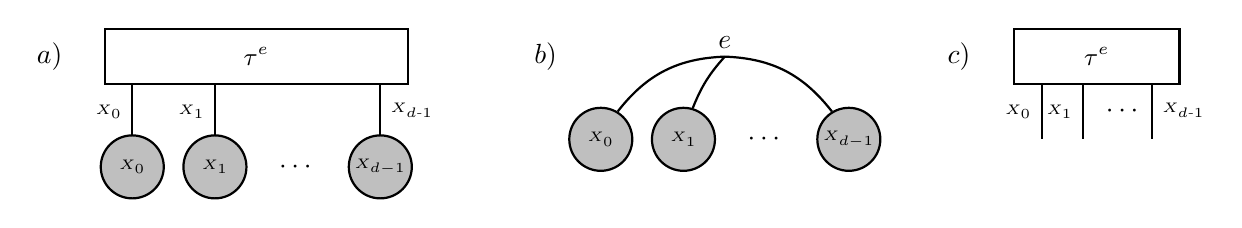
\begin{tikzpicture}[scale=0.35,thick] % , baseline = -3.5pt


\begin{scope}[shift={(-17,0)}]

\node[anchor=center] (text) at (-3,0) {$a)$};

\draw (-1,1) rectangle (10,-1);
\node[anchor=center] (text) at (4.5,0) {\corelabelsize $\hypercoreof{\edge}$};

\draw (0,-1)--(0,-3) node[midway,left] {\colorlabelsize $\catvariableof{0}$};
\draw (3,-1)--(3,-3) node[midway,left] {\colorlabelsize $\catvariableof{1}$};
\node[anchor=center] (text) at (3,-4) {$\cdots$};
\draw (9,-1)--(9,-3) node[midway,right] {\colorlabelsize $\catvariableof{\atomorder\shortminus1}$};

\node [circle, draw, thick, fill=\nodegrayscale, minimum size = \nodeminsize] (P1) at (0,-4) {\colorlabelsize $\catvariableof{0}$};
\node [circle, draw, thick, fill=\nodegrayscale, minimum size = \nodeminsize] (P2) at (3,-4) {\colorlabelsize $\catvariableof{1}$};
\node[anchor=center] (text) at (6,-4) {$\cdots$};

\node [circle, draw, thick, fill=\nodegrayscale, minimum size = \nodeminsize] (P3) at (9,-4) {};

\node[anchor=center] (text) at (9,-4) {\colorlabelsize $\catvariableof{\atomorder-1}$};


\end{scope}


\node[anchor=center] (text) at (-2,0) {$b)$};

\node [circle, draw, thick, fill=\nodegrayscale, minimum size = \nodeminsize] (P1) at (0,-3) {\colorlabelsize $\catvariableof{0}$};
\node [circle, draw, thick, fill=\nodegrayscale, minimum size = \nodeminsize] (P2) at (3,-3) {\colorlabelsize $\catvariableof{1}$};

\node[anchor=center] (text) at (6,-3) {$\cdots$};

\node [circle, draw, thick, fill=\nodegrayscale, minimum size = \nodeminsize] (P3) at (9,-3) {};

\node[anchor=center] (text) at (9,-3) {\colorlabelsize $\catvariableof{\atomorder-1}$};


\draw (P1) to[bend right=-25] (4.5,0);
\draw (P2) to[bend right=-10] (4.5,0);
\draw (P3) to[bend right=25] (4.5,0);
\node[anchor=center] (text) at (4.5,0.5) {$\edge$};


\begin{scope}[shift={(16,2)}]

\node[anchor=center] (text) at (-3,-2) {$c)$};

\draw (-1,-1) rectangle (5,-3);
\node[anchor=center] (text) at (2,-2) {\corelabelsize $\hypercoreof{\edge}$};
\draw (0,-3)--(0,-5) node[midway,left] {\colorlabelsize $\catvariableof{0}$};
\draw (1.5,-3)--(1.5,-5) node[midway,left] {\colorlabelsize $\catvariableof{1}$};
\node[anchor=center] (text) at (3,-4) {$\cdots$};
\draw (4,-3)--(4,-5) node[midway,right] {\colorlabelsize $\catvariableof{\atomorder\shortminus1}$};

\end{scope}

%\drawatomcore{3.5}{-8}{$\probtensor$}
%\drawatomindices{3.5}{-12}	
%\draw (5.5,-9)--(5.5,-7) node[midway,right] {\colorlabelsize $\catvariableof{\exformula}$};

\end{tikzpicture}
\end{center}
Drawing on the association of variables with nodes and of tensors with hyperedges build by the assigned variables we continue with the definition of tensor networks.

\begin{definition}[Tensor Network]
    \label{def:tensorNetwork}
    Let $\graph=(\nodes,\edges)$ be a hypergraph with nodes decorated by categorical variables $\catvariableof{\node}$ with dimensions $\catdimof{\node} \in \nn$
    and hyperedges $\edge\in\edges$ decorated by core tensors
    \[ \hypercoreofat{\edge}{\catvariableof{\edge}} \in \bigotimes_{\node\in\edge}\rr^{\catdimof{\node}} \, , \]
    where we denote by $\catvariableof{\edge}$ the set of categorical variables $\catvariableof{\node}$ with $\node\in\edge$.
    Then we call the set
    \[ \tnetofat{\graph}{\catvariableof{\nodes}} = \{\hypercoreofat{\edge}{\catvariableof{\edge}}  \wcols \edge\in\edges\} \]
    the Tensor Network of the decorated hypergraph $\graph$.
    The set of tensor networks on $\graph$, such that all tensors have non-negative coordinates, is denoted by $\tnsetof{\graph}$.
\end{definition}

As examples we now present the $\cpformat$ and the $\ttformat$ formats in our hypergraph notation.

\begin{example}[The $\cpformat$ format]
    The Candecomp-Parafac ($\cpformat$ (\cite{hitchcock_expression_1927}) tensor format corresponds in our notation with a hypergraph (see \figref{fig:CPHypergraph})
    \begin{itemize}
        \item Nodes by $\catvariableof{[\catorder]}$ and a single hidden variable $\decvariable$, decorated by dimensions $\catdimof{[\catorder]}$ and $\decdim$.
        \item Edges by
        \begin{align*}
            \left\{\edgeof{\catenumerator}=(\catvariableof{\catenumerator},\decvariable) \wcols \catenumeratorin \right\}
        \end{align*}
        each decorated by a matrix $\hypercoreofat{\edgeof{\catenumerator}}{\catvariableof{\catenumerator},\decvariable}$.
    \end{itemize}

    \begin{figure}
        \begin{center}
            \input{../tikz_pics/notation_basic_concepts/cp_hypergraph.tex}
        \end{center}
        \caption{Hypergraph to a $\cpformat$ format.
        a) Node-centric design.
        b) Corresponding tensor-network on the edges of the hypergraph.}\label{fig:CPHypergraph}
    \end{figure}

\end{example}

\begin{example}[The $\ttformat$ format]\label{exa:ttFormat}
    The Tensor-Train ($\ttformat$) format (see \cite{oseledets_tensor-train_2011}) corresponds in our notation to a hypergraph (see \figref{fig:TTHypergraph}) defined by
    \begin{itemize}
        \item nodes $\catvariableof{[\catorder]}$ and hidden variables $\decvariableof{[\catorder-1]}$, each decorated by a dimension $\catdimof{[\catorder]}$ and $\decdimof{[\catorder-1]}$,
        \item edges
        \begin{align*}
            \big\{\edgeof{0}=\{\catvariableof{0},\decvariableof{0}\}\big\} \cup
            \big\{\edgeof{\catenumerator}=\{\decvariableof{\catenumerator-1},\catvariableof{\catenumerator},\decvariableof{\catenumerator}\} \wcols \catenumerator\in\{1,\ldots,\catorder-2\}\big\} \cup
            \big\{\edgeof{\catorder-1}=\{\decvariableof{\catorder-2},\catvariableof{\catorder-1}\}\big\}
        \end{align*}
        each decorated by a tensor of order 3 (respectively 2 for $\catenumerator\in\{0,\seldim-1\}$).
    \end{itemize}
    \begin{figure}
        \begin{center}
            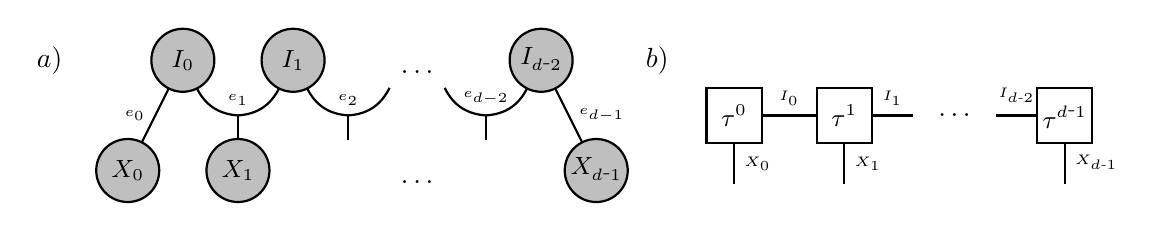
\begin{tikzpicture}[scale=0.35,thick]

                \begin{scope}[shift={(-22,-2)}]
                    \coordinate[label=left:$a)$] (A) at (-2,4);

                    \node[circle, draw, thick, fill=\nodegrayscale, minimum size = \nodeminsize] (A) at (0,0) {};
                    \node[anchor=center] (A) at (0,0) {\corelabelsize $\catvariableof{0}$};
                    \node[circle, draw, thick, fill=\nodegrayscale, minimum size = \nodeminsize] (A) at (4,0) {};
                    \node[anchor=center] (A) at (4,0) {\corelabelsize $\catvariableof{1}$};


                    \coordinate[label=below:$\hdots $] (A) at (10.5,4);
                    \coordinate[label=below:$\hdots $] (A) at (10.5,0);

                    \node[circle, draw, thick, fill=\nodegrayscale, minimum size = \nodeminsize] (A) at (2,4) {};
                    \node[anchor=center] (A) at (2,4) {\corelabelsize $\decvariableof{0}$};
                    \node[circle, draw, thick, fill=\nodegrayscale, minimum size = \nodeminsize] (A) at (6,4) {};
                    \node[anchor=center] (A) at (6,4) {\corelabelsize $\decvariableof{1}$};

                    %\coordinate[label=above:$e_0$] (A) at (0.5,1.6);
                    %\node[anchor=south] (A) at (0.5,1.6) {\colorlabelsize $e_0$};
                    \draw (0.5,1) -- (1.5,3) node[midway,left] {\colorlabelsize $e_0$};
%                    \draw (2,2)  to[bend right=30] (0.5,1);
%                    \draw (2,2)  to[bend left=30] (3.5,1);
%                    \draw (2,2) -- (2,2.9);

                    \node[anchor=south] (A) at (4,2) {\colorlabelsize $e_1$};
                    \draw (4,2)  to[bend right=-30] (2.5,3);
                    \draw (4,2)  to[bend left=-30] (5.5,3);
                    \draw (4,2) -- (4,1.1);

                    \node[anchor=south] (A) at (8,2) {\colorlabelsize $e_2$};
                    \draw (8,2)  to[bend right=-30] (6.5,3);
                    \draw (8,2)  to[bend left=-30] (9.5,3);
                    \draw (8,2) -- (8,1.1);

                    \begin{scope}[shift={(3,0)}]

                        \node[anchor=south] (A) at (10,2) {\colorlabelsize $e_{\catorder-2}$};
                        \draw (10,2)  to[bend right=-30] (8.5,3);
                        \draw (10,2)  to[bend left=-30] (11.5,3);
                        \draw (10,2) -- (10,1.1);

                        %\node[anchor=south] (A) at (0.5,1.6) {\colorlabelsize $e_0$};
                        \draw (13.5,1) -- (12.5,3) node[midway,right] {\colorlabelsize $e_{\catorder-1}$};

                        %\coordinate[label=above:$e_{\catorder-1}$] (A) at (11,1.6);
                        %\draw (12,2)  to[bend right=30] (10.5,1);
                        %\draw (12,2)  to[bend left=30] (13.5,1);
                        %\draw (12,2) -- (12,2.9);

                        \node[circle, draw, thick, fill=\nodegrayscale, minimum size = \nodeminsize] (A) at (12,4) {};
                        \node[anchor=center] (text) at (12,4) {\corelabelsize $\decvariableof{\catorder\shortminus2}$};

                        \node[circle, draw, thick, fill=\nodegrayscale, minimum size = \nodeminsize] (A) at (14,0) {};
                        \node[] (text) at (14,0) {\corelabelsize $\catvariableof{\catorder\shortminus1}$};
                    \end{scope}
                \end{scope}

                \coordinate[label=left:$b)$] (A) at (-2,2);

                \draw (-1,-1) rectangle (1,1);
                \node[anchor=center] (A) at (0,0) {\corelabelsize $\hypercoreof{0}$};
                \draw (0,-1)--(0,-2.5) node[midway,right] {\colorlabelsize $\catvariableof{0}$};

                \draw (1,0) -- (3,0) node[midway,above] {\colorlabelsize $\decvariableof{0}$};

                \draw (3,-1) rectangle (5,1);
                \node[anchor=center] (A) at (4,0) {\corelabelsize $\hypercoreof{1}$};
                \draw (4,-1)--(4,-2.5) node[midway,right] {\colorlabelsize $\catvariableof{1}$};

                \draw (5,0) -- (6.5,0) node[midway,above] {\colorlabelsize $\decvariableof{1}$};

%    \coordinate[label=below:$\hdots $] (A) at (9,0.35);
                \node[anchor=center] (text) at (8,0) {$\hdots$};

                \draw (9.5,0) -- (11,0) node[midway,above] {\colorlabelsize $\decvariableof{\catorder\shortminus2}$};;
                \draw (11,-1) rectangle (13,1);
                \node[anchor=center] (A) at (12,0) {\corelabelsize $\hypercoreof{\catorder\shortminus1}$};
                \draw (12,-1)--(12,-2.5) node[midway,right] {\colorlabelsize $\catvariableof{\catorder\shortminus1}$};


            \end{tikzpicture}
        \end{center}
        \caption{Hypergraph to a $\ttformat$ format.
        a) Node-centric design.
        b) Corresponding tensor-network on the edges of the hypergraph.}\label{fig:TTHypergraph}
    \end{figure}

\end{example}

\subsection{Generic Contractions}

Let us now exploit our graphical approach to tensor networks in the definition of contractions. % of tensor networks as operations to get single tensors from tensor networks. % by summing slices of tensors in a network over common variables.

\begin{definition}
    \label{def:contraction}
    Let $\tnetof{\graph}$ be a tensor network on a decorated hypergraph $\graph=(\nodes,\edges)$.
    For any subset $\secnodes\subset\nodes$ we define the contraction to be the tensor (for an example see \figref{fig:contraction})
    \begin{align}
        \contractionof{\tnetof{\graph}}{\secnodevariables} \in \bigotimes_{\node\in\secnodes} \rr^{\catdimof{\node}}
    \end{align}
    defined coordinatewise by the sum
    \begin{align}
        \contractionof{\tnetof{\graph}}{\indexedcatvariableof{\secnodes}} =
        \sum_{\catindexof{\nodes/\secnodes} \in\,\nodestatesof{\nodes/\secnodes}}
        \left( \prod_{\edge\in\edges}\hypercoreofat{\edge}{\indexedcatvariableof{\edge}} \right) \, .
    \end{align}
    We call $\secnodevariables$ the open variables of the contraction.
\end{definition}

% Open variables
%We here defined contractions formally by only specifying the open variables, where the connectivity of the tensors is clear from the shared variables.
When an open variable $\catvariable$ is not appearing at any tensor in a contraction, we define the contraction as a tensor product with the trivial tensor $\onesat{\catvariable}$.
To ease notation, we will often omit the set notation by brackets $\{\cdot\}$ and specify the tensors to be contracted with the delimiter "," (see e.g. \exaref{exa:matrixProduct}).

\begin{figure}
    \begin{center}
        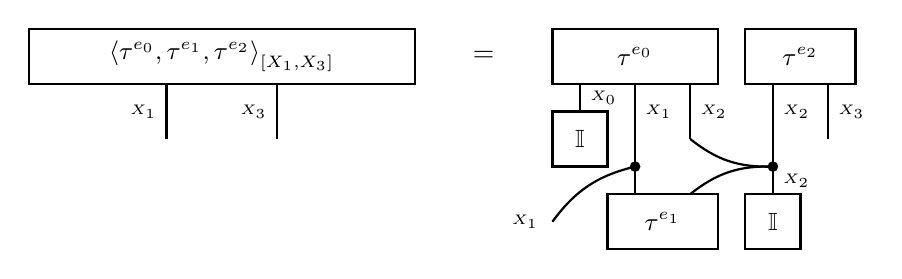
\begin{tikzpicture}[scale=0.35,thick]

    \draw (-5,-1) rectangle (9,-3);
    \node[anchor=center] (text) at (2,-2) {\corelabelsize $\contractionof{\hypercoreof{\edge_0},\hypercoreof{\edge_1},\hypercoreof{\edge_2}}{\catvariableof{1},\catvariableof{3}}$};
    \draw (0,-3)--(0,-5) node[midway,left] {\colorlabelsize $\catvariableof{1}$};
    \draw (4,-3)--(4,-5) node[midway,left] {\colorlabelsize $\catvariableof{3}$};

    \node[anchor=center] (text) at (11.5,-2) {${=}$};

    \begin{scope}
        [shift={(15,0)}]

        \draw (-1,-1) rectangle (5,-3);
        \node[anchor=center] (text) at (2,-2) {\corelabelsize $\hypercoreof{\edge_0}$};
        \draw (0,-3)--(0,-4) node[midway,right] {\colorlabelsize $\catvariableof{0}$};
        \draw (-1,-4) rectangle (1,-6);
        \node[anchor=center] (text) at (0,-5) {\corelabelsize $\ones$};

        \draw (2,-3)--(2,-5) node[midway,right] {\colorlabelsize $\catvariableof{1}$};
        \draw (4,-3)--(4,-5) node[midway,right] {\colorlabelsize $\catvariableof{2}$};


        \draw (6,-1) rectangle (10,-3);
        \node[anchor=center] (text) at (8,-2) {\corelabelsize $\hypercoreof{\edge_2}$};
        \draw (7,-3)--(7,-5) node[midway,right] {\colorlabelsize $\catvariableof{2}$};
        \draw (9,-3)--(9,-5) node[midway,right] {\colorlabelsize $\catvariableof{3}$};


        \draw (1,-7) rectangle (5,-9);
        \node[anchor=center] (text) at (3,-8) {\corelabelsize $\hypercoreof{\edge_1}$};
        \draw (2,-5)--(2,-7); % node[midway,left] {\colorlabelsize $\catvariableof{1}$};
        \draw (4,-5) to[bend right=20]  (7,-6); % node[midway,left] {\colorlabelsize $\catvariableof{2}$};
        \draw (4,-7) to[bend right=-20]  (7,-6);

        \draw[fill] (2,-6) circle (\dotsize);
        \draw (2,-6) to[bend right=20] (-1,-8); % node[midway, right]{\colorlabelsize $\catvariableof{1}$};
        \node[anchor=center] (text) at (-2,-8) {\colorlabelsize $\catvariableof{1}$};

        \draw[fill] (7,-6) circle (\dotsize);
        \draw (7,-5) -- (7,-6);
        \draw (7,-6)--(7,-7) node[midway,right] {\colorlabelsize $\catvariableof{2}$};

        \draw (6,-7) rectangle (8,-9);
        \node[anchor=center] (text) at (7,-8) {\corelabelsize $\ones$};

    \end{scope}


\end{tikzpicture}
    \end{center}
    \caption{
        Graphical depiction of a tensor network contraction with the open variables $\catvariableof{1},\catvariableof{3}$.
        Open variables are depicted by those without a dot at the end of the line.
    }\label{fig:contraction}
\end{figure}

\begin{example}[Tensor Product]
    The simplest contraction is the tensor product, which maps a pair of two tensors with distinct variables onto a third tensor and has an interpretation by coordinate wise products.
    Such a contraction corresponds with a tensor network of two tensors with disjoint variables.
    Let there be two tensors
    \begin{align*}
        \hypercoreat{\shortcatvariables} \in \facspace  \andspace \sechypercoreat{\secshortcatvariables} \in \secfacspace
    \end{align*}
    with different categorical variables assigned to its axes.
    Then their tensor product is the map
    \begin{align*}
        \contractionof{\hypercoreat{\shortcatvariables},\sechypercoreat{\secshortcatvariables}}{\shortcatvariables,\secshortcatvariables}
        \in \left(\facspace\right) \otimes \left(\secfacspace \right)
        %:  \left(\facstates\right) \times \left(\secfacstates\right) \rightarrow \rr
    \end{align*}
    defined coordinatewise for tuples of $\catindices\in\facstates$ and $\seccatindices\in\secfacstates$ as
    \begin{align*}
        & \contractionof{\hypercoreat{\shortcatvariables},\sechypercoreat{\secshortcatvariables}}{\indexedcatvariables,\indexedseccatvariables} \\
        &\quad\quad \coloneqq  \hypercoreat{\indexedcatvariables}\cdot \sechypercoreat{\indexedseccatvariables} \, .
    \end{align*}
\end{example}

\subsection{Normalizations}

%% Directionality by Normalization
\begin{definition}
    \label{def:normalization}
    The normalization of a tensor $\hypercorewithnodes$ on incoming nodes $\innodes\subset\nodes$ and outgoing nodes $\outnodes\subset\nodes/\innodes$ is the tensor $\normalizationofwrt{\hypercorewithnodes}{\catvariableof{\outnodes}}{\catvariableof{\innodes}}$ defined for $\catindexof{\innodes}$ as
    \begin{align*}
        \normalizationofwrt{\hypercorewithnodes}{\catvariableof{\outnodes}}{\indexedcatvariableof{\innodes}}
        = \begin{cases}
              \frac{\contractionof{\hypercore}{\catvariableof{\outnodes},\indexedcatvariableof{\innodes}}}{\contractionof{\hypercore}{\indexedcatvariableof{\innodes}}} & \ifspace \contractionof{\hypercore}{\indexedcatvariableof{\innodes}} \neq 0 \\
              \frac{1}{\prod_{\node\in\outnodes}\catdimof{\node}}\onesat{\catvariableof{\outnodes}} & \text{else}
        \end{cases} \, .
    \end{align*}
    We say that $\hypercorewithnodes$ is normalized with incoming nodes $\incomingnodes\subset\nodes$, if
    \begin{align*}
        \hypercorewithnodes
        = \normalizationofwrt{\hypercorewithnodes}{\catvariableof{\nodes/\innodes}}{\catvariableof{\innodes}} \, .
    \end{align*}
\end{definition}

%% Diagrammatic notation
In our graphical tensor notation, we depict normalized tensors by directed hyperedges (a), which are decorated by directed tensors (b), for example:
\begin{center}
    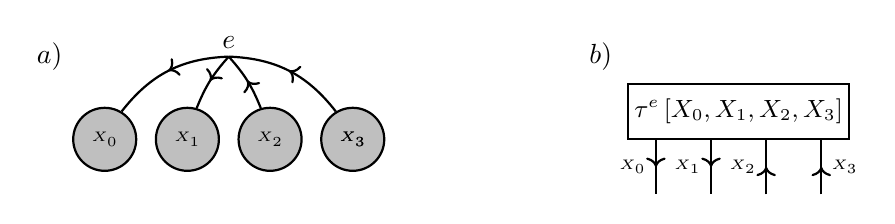
\begin{tikzpicture}[scale=0.35,thick] % , baseline = -3.5pt

    \node[anchor=center] (text) at (-2,0) {$a)$};

    \node [circle, draw, thick, fill=\nodegrayscale, minimum size = \nodeminsize] (P1) at (0,-3) {\colorlabelsize $\catvariableof{0}$};
    \node [circle, draw, thick, fill=\nodegrayscale, minimum size = \nodeminsize] (P2) at (3,-3) {\colorlabelsize $\catvariableof{1}$};

%\node[anchor=center] (text) at (6,-3) {$\cdots$};
    \node [circle, draw, thick, fill=\nodegrayscale, minimum size = \nodeminsize] (P3) at (6,-3)  {\colorlabelsize $\catvariableof{2}$};

    \node [circle, draw, thick, fill=\nodegrayscale, minimum size = \nodeminsize] (P4) at (9,-3)  {\colorlabelsize $\catvariableof{3}$};

    \node[anchor=center] (text) at (9,-3) {\colorlabelsize $\catvariableof{3}$};


    \draw[midarrow]
    (4.5,0) to[bend right=25] (P1);
    \draw[midarrow]
    (4.5,0) to[bend right=10] (P2);
    \draw[midarrow]
    (P3) to[bend right=10] (4.5,0);
    \draw[midarrow]
    (P4) to[bend right=25] (4.5,0);

    \node[anchor=center] (text) at (4.5,0.5) {$\edge$};


    \begin{scope}[shift={(20,0)}]

        \node[anchor=center] (text) at (-2,0) {$b)$};

        \draw (-1,-1) rectangle (7,-3);
        \node[anchor=center] (text) at (3,-2) {\corelabelsize $\hypercoreofat{\edge}{\catvariableof{0},\catvariableof{1},\catvariableof{2},\catvariableof{3}}$};
%\draw[->-] (0,-3)--(0,-5) node[midway,left] {\colorlabelsize $\catvariableof{0}$};
%\draw[->-] (1.5,-3)--(1.5,-5) node[midway,left] {\colorlabelsize $\catvariableof{1}$};
%\node[anchor=center] (text) at (3,-4) {$\cdots$};
%\draw[->-] (4,-3)--(4,-5) node[midway,right] {\colorlabelsize $\catvariableof{\atomorder-1}$};


        \draw[midarrow]  (0,-3) -- (0,-5) node[midway,left] {\colorlabelsize $\catvariableof{0}$};
        \draw[midarrow]
        (2,-3)--(2,-5) node[midway,left] {\colorlabelsize $\catvariableof{1}$};
        \draw[midarrow]
        (4,-5)--(4,-3) node[midway,left] {\colorlabelsize $\catvariableof{2}$};
        \draw[midarrow]
        (6,-5)--(6,-3) node[midway,right] {\colorlabelsize $\catvariableof{3}$};
    \end{scope}


\end{tikzpicture}
\end{center}

\subsection{Function encoding and \ComputationActivationNetworks{}}

Towards presenting the function encoding schemes we define one-hot encodings mapping the states of variables to basis tensors.

\begin{definition}[One-hot encodings to Factored Representations]
    \label{def:onehotenc}
    To any variable $\catvariable$ taking values in $[\catdim]$ the one-hot encoding of any state $\catindex\in[\catdim]$ is the vector with coordinates
    \begin{align}
        \onehotmapofat{\catindex}{\catvariable=\tilde{\catindex}}
        \coloneqq \begin{cases}
                      1 & \ifspace \catindex=\tilde{\catindex} \\
                      0 & \text{else} \, .
        \end{cases}
    \end{align}
    To any tuple $(\catvariables)$ of variables taking values in $\facstates$ the one-hot encoding of a state tuple $\shortcatindices=(\catindexof{0},\ldots,\catindexof{\catorder-1})$ is the tensor product
    \begin{align*}
        \onehotmapofat{\shortcatindices}{\shortcatvariables}
        \coloneqq \bigotimes_{\catenumeratorin} \onehotmapofat{\catindexof{\atomenumerator}}{\catvariableof{\atomenumerator}} \, .
    \end{align*}
\end{definition}

%The basis vectors $\onehotmapofat{\catindex}{\catvariable}$ are tensors of order $1$ and leg dimension $\catdim$ of the structure
%\begin{align}
%    \onehotmapofat{\catindex}{\catvariable}
%    = \begin{bmatrix}
%          0 & \cdots & 0 & 1 & 0 & \cdots & 0
%    \end{bmatrix}^T \, ,
%\end{align}
%where the $1$ is at the $\catindex$-th coordinate of the vector.

We now use one-hot encodings to encode functions between state sets.

\begin{definition}[Basis encoding of maps between state sets]
    \label{def:functionRepresentation}
    Let there be two systems with factored representations by variables $\shortcatvariables$ and $\headvariables$, and a map
    \begin{align*}
        \statesetfunction\defcols\facstates \rightarrow  \headstates
    \end{align*}
    between these state sets.
    Then the basis encoding of $\statesetfunction$ is a tensor
    \begin{align*}
        \bencodingofat{\statesetfunction}{\headvariables,\shortcatvariables}
        \in \left(\secfacspace\right) \otimes \left(\facspace\right)
    \end{align*}
    defined by
    \begin{align*}
        & \bencodingofat{\statesetfunction}{\headvariables,\shortcatvariables}
        \quad = \sum_{\catindices\in\facstates}
        \onehotmapofat{\statesetfunctionev{\shortcatindices}}{\headvariables} \otimes  \onehotmapofat{\shortcatindices}{\shortcatvariables} \, .
    \end{align*}
\end{definition}
Basis encodings are normalized tensors and are thus depicted as decorations of directed edges in hypergraphs:
\begin{center}
    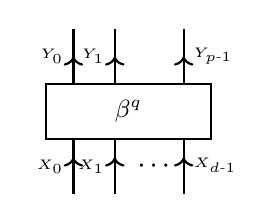
\begin{tikzpicture}[scale=0.35,thick] % , baseline = -3.5pt


    \draw[->-] (0,-1)--(0,1) node[midway,left] {\colorlabelsize $\headvariableof{0}$};
    \draw[->-] (1.5,-1)--(1.5,1) node[midway,left] {\colorlabelsize $\headvariableof{1}$};
    \node[anchor=center] (text) at (3,-4) {$\cdots$};
    \draw[->-] (4,-1)--(4,1) node[midway,right] {\colorlabelsize $\headvariableof{\seccatorder\shortminus1}$};

    \draw (-1,-1) rectangle (5,-3);
    \node[anchor=center] (text) at (2,-2) {\corelabelsize $\bencodingof{\statesetfunction}$};
    \draw[-<-] (0,-3)--(0,-5) node[midway,left] {\colorlabelsize $\catvariableof{0}$};
    \draw[-<-] (1.5,-3)--(1.5,-5) node[midway,left] {\colorlabelsize $\catvariableof{1}$};
    \node[anchor=center] (text) at (3,-4) {$\cdots$};
    \draw[-<-] (4,-3)--(4,-5) node[midway,right] {\colorlabelsize $\catvariableof{\atomorder\shortminus1}$};


%\drawatomcore{3.5}{-8}{$\probtensor$}
%\drawatomindices{3.5}{-12}	
%\draw (5.5,-9)--(5.5,-7) node[midway,right] {\colorlabelsize $\catvariableof{\exformula}$};

\end{tikzpicture}
\end{center}

% Image enumeration
We further generalize basis encodings to arbitrary functions between finite sets, by the use of image enumeration maps.
Given an arbitrary set $\arbset$ we say a map
\begin{align*}
    \indexinterpretation \defcols
    [\cardof{\arbset}] \rightarrow \arbset
\end{align*}
is an enumeration map for $\arbset$.
Given a function $\exfunction:\inset\rightarrow\outset$ between arbitrary sets, and enumerating maps $\indexinterpretationof{\insymbol}$ and $\indexinterpretationof{\outsymbol}$ for both sets we define the basis encoding of $\exfunction$ as
\begin{align*}
    \bencodingofat{\exfunction}{\indvariableof{\outsymbol},\indvariableof{\insymbol}}
    = \sum_{\arbelement\in\inset} \onehotmapofat{\invindexinterpretationofat{\outsymbol}{\exfunction(\arbelement)}}{\indvariableof{\outsymbol}}
    \otimes \onehotmapofat{\invindexinterpretationofat{\insymbol}{\arbelement}}{\indvariableof{\insymbol}} \, ,
\end{align*}
where $\indvariableof{\insymbol},\indvariableof{\outsymbol}$ are variables taking values in $[\cardof{\inset}]$ and $[\cardof{\outset}]$.
%
Based on these concepts the main architecture can be defined.

\begin{definition}[\ComputationActivationNetwork{} (\CompActNets{})]
    \label{def:realizableStatDistributions}
    Given a function $\sstat : \facstates \rightarrow \parspace$, and a hypergraph $\graph=(\nodes,\edges)$ with nodes $[\seldim]\subset\nodes$ containing the image coordinates of $\sstat$, we define the by $\sstat$ computable and by $\graph$ activated family of distributions by
    \begin{align*}
        \realizabledistsof{\sstat,\graph}
        = \left\{ \normalizationof{\bencodingofat{\sstat}{\headvariables,\shortcatvariables},\contractionof{\acttensor}{\headvariables} %\} \cup \{\hypercoreofat{\edge}{\sstatcatof{\edge}} \wcols \edgein \}
        }{\shortcatvariables}
              \wcols \acttensorat{\headvariableof{\nodes}} \in \tnsetof{\graph} \right\} \, .
    \end{align*}
    We refer to any member $\probat{\shortcatvariables}\in\realizabledistsof{\sstat,\graph}$ as a \emph{\ComputationActivationNetwork{}} (\emph{\CompActNet{}}).
    We call $\bencsstatwith$ (and any decomposition of it) as the \emph{computation network} and by $\acttensorat{\headvariableof{\nodes}}$ as the \emph{activation network}.
\end{definition}
%\section{Decomposition of Probability Distributions}
\section{The Probabilistic Paradigm}\label{sec:probPar}

We here investigate tensor network decomposition mechanisms of probability distributions.
After introducing probability distributions as tensors we derive tensor network decompositions based on conditional independencies (applying the Hammersley-Clifford theorem \cite{clifford_markov_1971}) to motivate graphical models.
Further we present the \ComputationMechanism{}, in which the Fisher-Neyman Factorization Theorem is used to decompose distributions in the presence of sufficient statistics.

\subsection{Basic concepts}

As defined next, distributions $\probtensor$ over a discrete state space can be represented by tensors, where each entry corresponds to the probability of a corresponding state.

\begin{definition}[Joint Probability Distribution]
    \label{def:probabilityDistribution} % From the axioms of Kolmogorov!
    Let there be for each $\catenumeratorin$ a categorical variable $\catvariableof{\catenumerator}$ taking values in $[\catdimof{\atomenumerator}]$.
    A joint probability distribution of these categorical variables is a function
    \begin{align*}
        \probwith \defcols \facstates \rightarrow \rr
    \end{align*}
    which is non-negative, that is for any $\shortcatindicesin$ it holds
    \begin{align*}
        \probat{\indexedshortcatvariables} \geq 0 \, ,
    \end{align*}
    and which is normalized, that is
    \begin{align*}
        \contraction{\probat{\shortcatvariables}} = 1 \, .
    \end{align*}
    Let $\thirdcatvariable$ be another variable taking values in a possibly infinite set $\mathrm{val}(\thirdcatvariable)$.
    Then a tensor $\condprobat{\shortcatvariables}{\thirdcatvariable}$ is a family of joint probability distributions, if for any $\thirdcatindex\in\mathrm{val}(\thirdcatvariable)$ the slice $\condprobat{\shortcatvariables}{\thirdcatvariable=\thirdcatindex}$ is a joint probability distribution.
\end{definition}

\begin{example}[Family of independent coin tosses]
    Consider tossing a coin with head probability $\thirdcatindex\in[0,1]$ and repeating the experiment independently $\catorder\in\nn$ times.
    We define a variable $\thirdcatvariable$ taking values in $\mathrm{val}(\thirdcatvariable)=[0,1]$ and denote by $\shortcatvariables$ $\catorder$ boolean variables.
    Then, the family of coin toss distributions is the tensor $\condprobat{\shortcatvariables}{\thirdcatvariable}$ with coordinates $\shortcatindices\in\atomstates$ and $\thirdcatindex\in[0,1]$ defined by
    \begin{align*}
        \condprobat{\indexedshortcatvariables}{\thirdcatvariable=\thirdcatindex}
        = \prod_{\catenumeratorin} \thirdcatindex^{\catindexof{\catenumerator}} (1-\thirdcatindex)^{1-\catindexof{\catenumerator}}
        = \thirdcatindex^{\sum_{\catenumeratorin} \catindexof{\catenumerator}} (1-\thirdcatindex)^{\catorder - \sum_{\catenumeratorin} \catindexof{\catenumerator}} \, .
    \end{align*}
    Note that for each slice with respect to $\thirdcatindex\in[0,1]$ by the binomial theorem we have $\contraction{\probat{\shortcatvariables,\thirdcatvariable=\thirdcatindex}}=1$ and thus $\probat{\shortcatvariables,\thirdcatvariable}$ is indeed a family of probability distributions.
    For $\catorder=2$ we have more explicitly for any $\thirdcatindex\in[0,1]$ that
    \begin{center}
        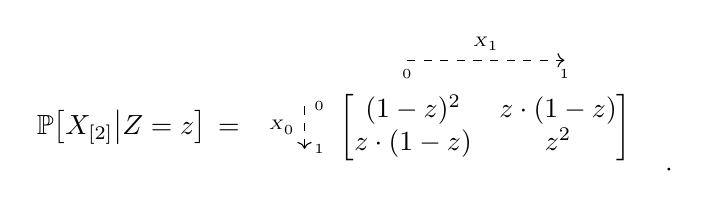
\begin{tikzpicture}[scale=1]
            \node[anchor=east] (A) at (-2,0) {$\condprobat{\catvariableof{[2]}}{\thirdcatvariable=\thirdcatindex}\,=$};

            \node (A) at (1,0) {
                $\begin{bmatrix}
                (1-\thirdcatindex)
                     ^2 & \thirdcatindex \cdot (1-\thirdcatindex) \\
                     \thirdcatindex \cdot (1-\thirdcatindex) & \thirdcatindex^2
                \end{bmatrix}$
            };
            \draw[<-,dashed] (-1.3,-0.275) node[right] {\tiny $1$} -- (-1.3,0.275) node [midway, left] {\tiny $\catvariableof{0}$} node[right] {\tiny $0$};
            \draw[->,dashed] (0,0.85) node[below] {\tiny $0$} -- (2,0.85) node [midway, above] {\tiny $\catvariableof{1}$} node[below] {\tiny $1$};
            \node[anchor=east] (A) at (3.5,-0.55) {$\cdot$};
        \end{tikzpicture}
    \end{center}
\end{example}

A basic inference operation on probability distributions is the computation of marginal and conditional distribution.

\begin{definition}\label{def:marginalConditionalDistribution}
    For any distribution $\probat{\catvariable,\seccatvariable}$ the marginal distribution is given by the contraction
    \begin{align*}
        \probat{\catvariable} \coloneqq \contractionof{\probat{\catvariable,\seccatvariable}}{\catvariable}
    \end{align*}
    which is depicted by the diagram
    \begin{center}
        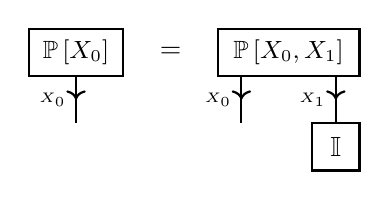
\begin{tikzpicture}[scale=0.3,thick] % , baseline = -3.5pt

\draw (-19,-1) rectangle (-15,-3);
\node[anchor=center] (text) at (-17,-2) {\corelabelsize $\margprobat{\exrandom}$};
\draw[midarrow]  (-17,-3)--(-17,-5) node[midway,left] {\colorlabelsize $\exrandom$};

\node[anchor=center] (text) at (-13,-2) {${=}$};

\draw (-11,-1) rectangle (-5,-3);
\node[anchor=center] (text) at (-8,-2) {\corelabelsize $\probat{\exrandom,\secexrandom}$};
\draw[midarrow]  (-10,-3)--(-10,-5) node[midway,left] {\colorlabelsize $\exrandom$};
\draw[midarrow]  (-6,-3)--(-6,-5) node[midway,left] {\colorlabelsize $\secexrandom$};
\draw (-7,-5) rectangle (-5,-7); 
\node[anchor=center] (text) at (-6,-6) {$\ones$};

\end{tikzpicture}
    \end{center}
    The conditional distribution of $\catvariable$ on $\seccatvariable$ is a tensor $\condprobat{\catvariable}{\seccatvariable}$ defined for $\seccatindex\in[\catdimof{1}]$
    \begin{align*}
        \condprobat{\catvariable}{\seccatvariable=\seccatindex} \coloneqq
        \begin{cases}
            \frac{1}{\catdim} \cdot \onesat{\catvariable} & \ifspace \contraction{\probat{\catvariable,\seccatvariable=\seccatindex}} = 0 \\
            \frac{1}{\contraction{\probat{\catvariable,\seccatvariable=\seccatindex}}} \cdot \probat{\catvariable,\seccatvariable=\seccatindex} & \text{else}
        \end{cases} \,
    \end{align*}
    and in the second case depicted by the diagram
    \begin{center}
        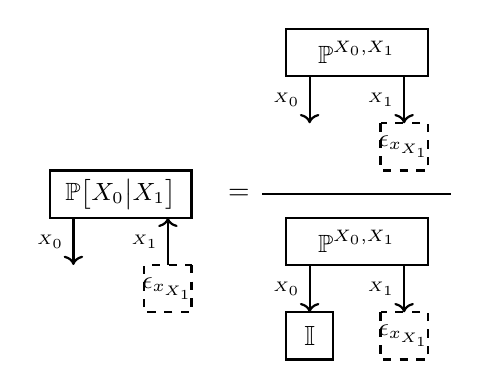
\begin{tikzpicture}[scale=0.3, thick] % , baseline = -3.5pt

\draw (-21,-1) rectangle (-15,-3);
\node[anchor=center] (text) at (-18,-2) {\small $\condprobof{\exrandom}{\secexrandom}$};
\draw[->]  (-20,-3)--(-20,-5) node[midway,left] {\tiny $\exrandom$}; 

\draw[<-]  (-16,-3)--(-16,-5) node[midway,left] {\tiny $\secexrandom$}; 
\draw[dashed] (-15,-5) rectangle (-17,-7); 
\node[anchor=center] (text) at (-16,-6) {\small $\onehotmapof{\catindexof{\secexrandom}}$};

\node[anchor=center] (text) at (-13,-2) {${=}$};


\begin{scope}[shift={(0,6)}]

\draw (-11,-1) rectangle (-5,-3);
\node[anchor=center] (text) at (-8,-2) {\small $\probof{\exrandom,\secexrandom}$};
\draw[->]  (-10,-3)--(-10,-5) node[midway,left] {\tiny $\exrandom$}; 
\draw[->]  (-6,-3)--(-6,-5) node[midway,left] {\tiny $\secexrandom$};
\draw[dashed] (-7,-5) rectangle (-5,-7); 
\node[anchor=center] (text) at (-6,-6) {\small $\onehotmapof{\catindexof{\secexrandom}}$};

\end{scope}

\draw (-12,-2) -- (-4,-2);

\begin{scope}[shift={(0,-2)}]

\draw (-11,-1) rectangle (-5,-3);
\node[anchor=center] (text) at (-8,-2) {\small $\probof{\exrandom,\secexrandom}$};
\draw[->]  (-10,-3)--(-10,-5) node[midway,left] {\tiny $\exrandom$}; 
\draw (-11,-5) rectangle (-9,-7); 
\node[anchor=center] (text) at (-10,-6) {$\ones$};
\draw[->]  (-6,-3)--(-6,-5) node[midway,left] {\tiny $\secexrandom$};
\draw[dashed] (-7,-5) rectangle (-5,-7); 
\node[anchor=center] (text) at (-6,-6) {\small $\onehotmapof{\catindexof{\secexrandom}}$};

\end{scope}

\end{tikzpicture}
    \end{center}
\end{definition}


% \textcolor{gray}{One of them is by employing the chain rule.
% \begin{theorem}[Chain Rule]
%     \label{the:chainRule}
%     For any probability distribution $\probwith$ we have
%     \begin{align*}
%         \probat{\shortcatvariables}
%         = \contractionof{\{\margprobat{\catvariableof{0}}\} \cup
%         \left\{\condprobof{\catvariableof{\catenumerator}}{\catvariableof{0},\ldots,\catvariableof{\catenumerator-1}} \wcols \catenumeratorin \ncond \catenumerator\geq 1\right\}
%         }{\shortcatvariables} \, ,
%     \end{align*}
%     provided that all conditional probability distributions exist.
% \end{theorem}
% \textcolor{darkgray}{ graphical notation of chain rule/Markov chain?}
% In case of Markov chains, where each random variable only depends on the previous random variable, this leads to a efficient representation.
% In general, the chain rule does not lead to a complexity reduction as the distribution $\condprobof{\catvariableof{\catenumerator}}{\catvariableof{0},\ldots,\catvariableof{\catenumerator-1}}$ has the same dimensions as the original probability distribution $\probat{\shortcatvariables}$.
% Therefore, other decompositions can be considered.
% }
% \alex{Its important to note, that the chain rule for itself does not provide a more efficient representation of the distribution (since it is a generic decomposition). 
% To achieve efficient tensor network decomposition, one needs to combine that with conditional independence assumptions (as in the Markov Chain case), such that conditioned variables in the conditional probability distributions can be dropped.}

\subsection{The Independence Mechanism: Graphical Model Factorization}

%% Need for decomposition mechanisms: Motivation for independence considerations
The number of coordinates in a tensor representation of probability distributions is the product
\begin{align*}
    \prod_{\catenumeratorin}\catdimof{\catenumerator} \, ,
\end{align*}
and therefore scales exponentially in the number of coordinates.
To find efficient representation schemes of probability distributions by tensor networks, we need to exploit additional properties of the distribution.
%% Independence
Independence leads to severe sparsifications of conditional probabilities and is therefore the key assumption to gain sparse decompositions of probability distributions.

%Markov Networks on hypergraphs $\graph$ are exactly those \CompActNets{}, which are computable with respect to the identity and the graph $\graph$.
%We here show how the sets of Markov Networks can be characterized by conditional independence assumptions.
%\alex{We can present graphical models and independences as decomposition schemes of activation tensors.
%Usually in graphical models there are no computation cores, hence the "features" of the statistic are the same as the variables.
%In that case the activation tensor is the same as the joint distribution tensor, that is a contraction of tensors colored by subsets of the variables (building the edges of the graphical models).

\begin{definition}[Independence]
    \label{def:independence} %% Was {the:independenceProductCriterion} in the report!
    We say that $\catvariableof{0}$ is independent of $\catvariableof{1}$ with respect to a distribution $\probat{\catvariableof{0},\catvariableof{1}}$, if the distribution is the tensor product of the marginal distributions, that is
    \begin{align*}
        \probat{\catvariableof{0},\catvariableof{1}}
        = \probat{\catvariableof{0}} \otimes \probat{\catvariableof{1}} \, .
    \end{align*}
    In this case we denote $\independent{\catvariableof{0}}{\catvariableof{1}}$.
\end{definition}

Thus, independence appears directly as a tensor–product decomposition of probability distribution.
Using tensor network diagrams we depict this property by
\begin{center}
    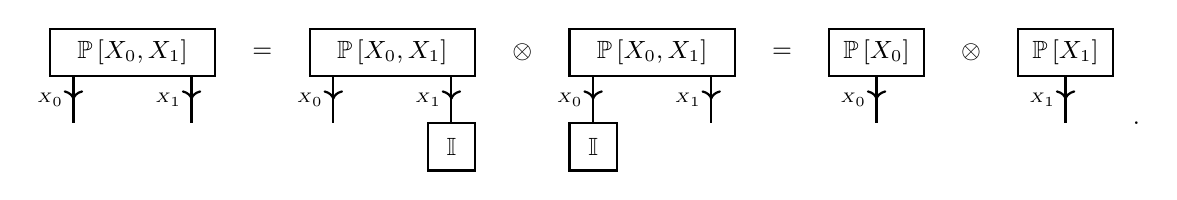
\begin{tikzpicture}[scale=0.3,thick] % , baseline = -3.5pt


\draw (0,1) rectangle (7,-1);
\node[anchor=center] (text) at (3.5,0) {\corelabelsize $\probat{\exrandom,\secexrandom}$};
\draw[->-] (1,-1) -- (1,-3) node[midway, left] {\colorlabelsize $\exrandom$};
\draw[->-] (6,-1) -- (6,-3) node[midway, left] {\colorlabelsize $\secexrandom$};

\node[anchor=center] (text) at (9,0) {\corelabelsize ${=}$};


\begin{scope}[shift={(11,0)}]

\draw (0,1) rectangle (7,-1);
\node[anchor=center] (text) at (3.5,0) {\corelabelsize $\probat{\exrandom,\secexrandom}$};
\draw[->-] (1,-1) -- (1,-3) node[midway, left] {\colorlabelsize $\exrandom$};
\draw[->-] (6,-1) -- (6,-3) node[midway, left] {\colorlabelsize $\secexrandom$};
\draw (5,-3) rectangle (7,-5);
\node[anchor=center] (text) at (6,-4) {\corelabelsize $\ones$};

\end{scope}

\node[anchor=center] (text) at (20,0) {\corelabelsize $\otimes$};

\begin{scope}[shift={(22,0)}]

\draw (0,1) rectangle (7,-1);
\node[anchor=center] (text) at (3.5,0) {\corelabelsize $\probat{\exrandom,\secexrandom}$};
\draw[->-] (1,-1) -- (1,-3) node[midway, left] {\colorlabelsize $\exrandom$};
\draw (0,-3) rectangle (2,-5);
\node[anchor=center] (text) at (1,-4) {\corelabelsize $\ones$};
\draw[->-] (6,-1) -- (6,-3) node[midway, left] {\colorlabelsize $\secexrandom$};

\end{scope}

\node[anchor=center] (text) at (31,0) {\corelabelsize ${=}$};

\begin{scope}[shift={(33,0)}]

\draw (0,1) rectangle (4,-1);
\node[anchor=center] (text) at (2,0) {\corelabelsize $\margprobat{\exrandom}$};
\draw[->-] (2,-1) -- (2,-3) node[midway, left] {\colorlabelsize $\exrandom$};

\node[anchor=center] (text) at (6,0) {\corelabelsize $\otimes$};

\draw (8,1) rectangle (12,-1);
\node[anchor=center] (text) at (10,0) {\corelabelsize $\margprobat{\secexrandom}$};
\draw[->-] (10,-1) -- (10,-3) node[midway, left] {\colorlabelsize $\secexrandom$};


\end{scope}

\node[anchor=center] (text) at (46,-3) {\corelabelsize ${.}$};

\end{tikzpicture} 
\end{center}
Let us notice, that the assumption of independence reduces the degrees of freedom from $\exranddim\cdot\secexranddim-1$ to $(\exranddim-1)+(\secexranddim-1)$.
The decomposition into marginal distributions furthermore exploits this reduced freedom and provides an efficient storage.
Having a joint distribution of multiple variables, which disjoint subsets are independent, we can iteratively apply the decomposition scheme.
As a result, we can reduce the scaling of the degrees of freedom from exponential to linear by the assumption of independence.

% Weakening of independence to conditional independence
Independence is, as we observed, a strong assumption, which is often too restrictive.
Conditional independence instead is a less demanding assumption, which still implies efficient tensor network decompositions schemes.
We introduce conditional independence as independence of variables with respect to conditional distributions.

\begin{definition}[Conditional Independence]
    \label{def:condIndependence} %% Was {the:condIndependenceProductCriterion} in the report!
    Given a joint distribution of variables $\catvariableof{0}$, $\catvariableof{1}$ and $\catvariableof{2}$, such that $\margprobat{\catvariableof{2}}$ is positive.
    We say that $\catvariableof{0}$ is independent of $\catvariableof{1}$ conditioned on $\catvariableof{2}$ if for any states $\exrandindin,\secexrandindin$ and $\thirdexrandindin$
    \begin{align*}
        \condprobof{\catvariableof{0},\catvariableof{1}}{\catvariableof{2}}
        = \contractionof{
            \condprobof{\catvariableof{0}}{\catvariableof{2}},\condprobof{\catvariableof{1}}{\catvariableof{2}}
        }{\catvariableof{0},\catvariableof{1},\catvariableof{2}} \, .
    \end{align*}
    In this case we denote $\condindependent{\catvariableof{0}}{\catvariableof{1}}{\catvariableof{2}}$.
\end{definition}

Conditional independence stated in \defref{def:condIndependence} has a close connection with independence stated in \defref{def:independence}.
To be more precise, $\catvariableof{0}$ is independent of $\catvariableof{1}$ conditioned on $\catvariableof{2}$, if and only if $\catvariableof{0}$ is independent of $\catvariableof{1}$ with respect to any slice $\condprobof{\catvariableof{0},\catvariableof{1}}{\indexedcatvariableof{2}}$ of the conditional distribution $\condprobof{\catvariableof{0},\catvariableof{1}}{\catvariableof{2}}$.

We can further exploit conditional independence to find tensor network decompositions of probabilities, as we show as the next corollary.
\begin{corollary}% NEEDED?
    \label{cor:secCriterionCondIndepencence}
    Let $\probat{\catvariableof{0},\catvariableof{1},\catvariableof{2}}$ be a joint distribution.
    If and only if $\catvariableof{0}$ is independent of $\catvariableof{1}$ conditioned on $\catvariableof{2}$ the distribution satisfies
    \begin{align*}
        \probat{\catvariableof{0},\catvariableof{1},\catvariableof{2}}
        = \contractionof{\condprobof{\catvariableof{0}}{\catvariableof{2}},\condprobof{\catvariableof{1}}{\catvariableof{2}},\margprobat{\catvariableof{2}}}{\catvariableof{0},\catvariableof{1},\catvariableof{2}} \, .
    \end{align*}
    In a diagrammatic notation this is depicted by
    \begin{center}
        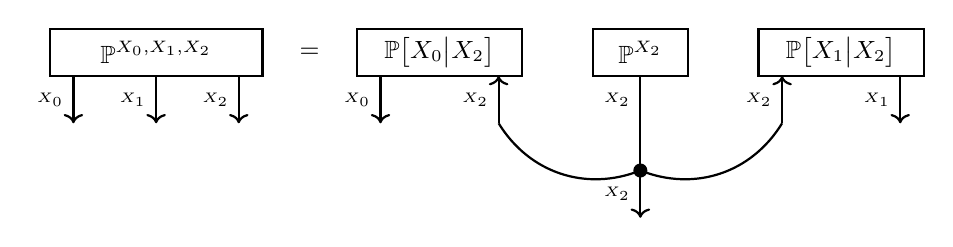
\begin{tikzpicture}[scale=0.3,thick] % , baseline = -3.5pt


\draw (-2,1) rectangle (7,-1);
\node[anchor=center] (text) at (2.5,0) {\small $\probof{\exrandom,\secexrandom,\thirdexrandom}$};
\draw[->] (-1,-1) -- (-1,-3) node[midway, left] {\tiny $\exrandom$};
\draw[->] (2.5,-1) -- (2.5,-3) node[midway, left] {\tiny $\secexrandom$};
\draw[->] (6,-1) -- (6,-3) node[midway, left] {\tiny $\thirdexrandom$};

\node[anchor=center] (text) at (9,0) {\small ${=}$};

\draw (11,1) rectangle (18,-1);
\node[anchor=center] (text) at (14.5,0) {\small $\condprobof{\exrandom}{\thirdexrandom}$};
\draw[->] (12,-1) -- (12,-3) node[midway, left] {\tiny $\exrandom$};
\draw[<-] (17,-1) -- (17,-3) node[midway, left] {\tiny $\thirdexrandom$};

\draw (21,1) rectangle (25,-1);
\node[anchor=center] (text) at (23,0) {\small $\probof{\thirdexrandom}$};
\draw (23,-1) -- (23,-3) node[midway, left] {\tiny $\thirdexrandom$};

\draw (23,-3) -- (23,-5);
\draw[fill] (23,-5) circle (0.25cm);
\draw[->] (23,-5) -- (23,-7) node[midway, left] {\tiny $\thirdexrandom$};
\draw (17,-3) to[bend right=40] (23,-5);
\draw (29,-3) to[bend right=-40] (23,-5);


\draw (28,1) rectangle (35,-1);
\node[anchor=center] (text) at (31.5,0) {\small $\condprobof{\secexrandom}{\thirdexrandom}$};
\draw[<-] (29,-1) -- (29,-3) node[midway, left] {\tiny $\thirdexrandom$};
\draw[->] (34,-1) -- (34,-3) node[midway, left] {\tiny $\secexrandom$};



\end{tikzpicture} 
    \end{center}
\end{corollary}

This conditional–independence pattern is the basic local building block that is generalized in Markov networks, which we define in the following.

\begin{definition}[Markov Network]
    \label{def:markovNetwork}
    Let $\tnetof{\graph}$ be a tensor network of non-negative tensors decorating a hypergraph $\graph$.
    Then the Markov Network $\probof{\graph}$ to $\tnetof{\graph}$ is the probability distribution of $\catvariableof{\node}$ defined by the tensor
    \begin{align*}
        \probofat{\graph}{\nodevariables} = \frac{
            \contractionof{\{\hypercoreof{\edge} \wcols \edgein\}}{\nodevariables}
        }{
            \contraction{\{\hypercoreof{\edge} \wcols \edgein\}}
        } = \normalizationof{\tnetof{\graph}}{\nodevariables} \, .
    \end{align*}
    We call the denominator
    \begin{align*}
        \partitionfunctionof{\tnetof{\graph}} = \contraction{\{\hypercoreof{\edge} \wcols \edgein\}}
    \end{align*}
    the partition function of the tensor network $\tnetof{\graph}$.
\end{definition}

%% Graphical Models as Tensor Networks: Alternative approach via graph duality
We define graphical models based on hypergraphs, to establish a direct connection with tensor network decorating the hypergraph.
In a more canonical way, Markov Networks are instead defined by graphs, where instead of the edges the cliques are decorated by factor tensors (see for example \cite{koller_probabilistic_2009}).
The probabilistic graphical models are along that alternative dual to tensor networks \cite{robeva_duality_2019,glasser_expressive_2019}.

%% CompActNets as Markov Networks - Check for redundancy!
We can interpret the factors $\hypercorewith$ as activation cores placed on the hyperedges $\edge$ of the graph.
The global activation tensor (and hence the joint distribution) is obtained by contracting this activation network and normalizing by its partition function.

%
While we so far have defined Markov Networks as decomposed probability distributions, we now want to derive assumptions on a distribution assuring that such decompositions exist.
As we will see, the sets of conditional independencies encoded by a hypergraph are captured by its separation properties, as we define next.

\begin{definition}[Separation of Hypergraph]
    A path in a hypergraph is a sequence of nodes $\node_{\atomenumerator}$ for $\atomenumeratorin$, such that for any $\atomenumerator\in[\atomorder-1]$ we find a hyperedge $\edgein$ such that $(\node_{\atomenumerator}, \node_{\atomenumerator+1})\subset \edge$.
    Given disjoint subsets $\nodesa$, $\nodesb$, $\nodesc$ of nodes in a hypergraph $\graph$ we say that $\nodesc$ separates $\nodesa$ and $\nodesb$ with respect to $\graph$, when any path starting at a node in $\nodesa$ and ending in a node in $\nodesb$ contains a node in $\nodesc$.
\end{definition}

To characterize Markov Networks in terms of conditional independencies we need to further define the property of clique-capturing.
This property of clique-capturing established a correspondence of hyperedges with maximal cliques in the more canonical graph-based definition of Markov Networks \cite{koller_probabilistic_2009}.

\begin{definition}[Clique-Capturing Hypergraph]
    \label{def:ccHypergraph}
    We call a hypergraph $\graph$ \emph{clique-capturing}, when each subset $\secnodes\subset\nodes$ is contained in a hyperedge, if for any $\nodea,\nodeb\in\secnodes$ there is a hyperedge $\edgein$ with $\nodea,\nodeb\in\secnodes$.
\end{definition}

Let us now show a characterization of Markov Networks in terms of conditional independencies.

% Characterization
\begin{theorem}[Hammersley-Clifford Factorization Theorem]
    \label{the:factorizationHammersleyClifford}
    Let there be a positive probability distribution $\probwithnodes$ and a clique-capturing hypergraph $\graph=(\nodes,\edges)$.
    Then the following are equivalent:
    \begin{itemize}
        \item[i] The distribution $\probwithnodes$ is representable by a Markov Network on $\graph$, i.e. for each edge $\edgein$ there is a tensor $\hypercoreofat{\edge}{\catvariableof{\edge}}$ such that
        \begin{align*}
            \probwithnodes = \normalizationof{\{\hypercoreofat{\edge}{\catvariableof{\edge}}\wcols\edgein\}}{\nodevariables}
        \end{align*}
        \item[ii] For any subsets $\nodesa,\nodesb,\nodesc\subset\nodes$ such that $\nodesc$ separates $\nodesa$ from $\nodesb$, we have
        \begin{align*}
            \condindependent{\catvariableof{\nodesa}}{\catvariableof{\nodesb}}{\catvariableof{\nodesc}} \, .
        \end{align*}
    \end{itemize}
    %Given a clique-capturing hypergraph $\graph$, the set of positive Markov Networks on the hypergraph coincides with the set of positive probability distributions, such that for each disjoint subsets of variables $\nodesa$, $\nodesb$, $\nodesc$ we have $\catvariableof{\nodesa}$ is independent of $\catvariableof{\nodesb}$ conditioned on $\catvariableof{\nodesc}$, when $\nodesc$ separates $\nodesa$ and $\nodesb$ in the hypergraph. % called d-separation
\end{theorem}
\begin{proof}
    Shown in Appendix~\secref{sec:proofFactorizationTheorems}.
\end{proof}

By \theref{the:factorizationHammersleyClifford} the conditional independence structure of $\probwithnodes$ determines a global tensor network decomposition of $\probwithnodes$.
We refer to this correspondence between independence structure and tensor network factorization as the \emph{\independenceMechanism{}}.
Note, that the assumption of a positive distribution is required (i.e. for all $\shortcatindices$ we have $\probat{\indexedshortcatvariables}>0$).
The assumption of positivity was however not required in our characterization of independencies and conditional independencies by the existence of corresponding tensor decompositions (see \defref{def:independence} and \defref{def:condIndependence}).

\begin{example}[I.i.d. Boolean Variables: Coin toss interpretation]\label{exa:ctHc}
    Let there be $\catorder$ boolean variables $\shortcatvariables$, which are i.i.d. drawn from a positive distribution $\probat{\catvariable}$.
    From the pairwise independencies of $\catvariableof{\catenumerator}$ it follows with the Hammersley-Clifford Factorization Theorem that the distribution is representable by an elementary tensor network, that is
    \begin{align*}
        \probwith = \bigotimes_{\catenumeratorin} \probat{\catvariableof{\catenumerator}} \, .
    \end{align*}
\end{example}

\input{../examples/probabilistic_paradigm/student_hc}

\subsection{The Computation Mechanism: Factorization in presense of Sufficient Statistics}

We now present the \computationMechanism{} of finding tensor network decompositions of probability distributions.

\begin{definition}
    \label{def:sufStatistic}
    Let $\probat{\catvariable,\thirdcatvariable}$ be a joint distribution of the $\catdim$-dimensional variable $\catvariable$ and the $\thirdcatdim$-dimensional variable $\thirdcatvariable$ and let
    \begin{align*}
        \sstat \defcols [\catdim] \rightarrow [\headdim]
    \end{align*}
    be a statistic.
    We are interested in the distribution $\probat{\catvariable,\thirdcatvariable,\headvariableof{\sstat}}=\contractionof{\probat{\catvariable,\thirdcatvariable},\bencodingofat{\sstat}{\headvariableof{\sstat},\catvariable}}{\catvariable,\thirdcatvariable,\headvariableof{\sstat}}$.
    We say that $\sstat$ is a sufficient statistic for $\thirdcatvariable$ if and only if $\catvariable$ is independent of $\thirdcatvariable$ conditioned on $\headvariableof{\sstat}$.
\end{definition}

Note that the independence in \defref{def:sufStatistic} is true if and only if
\begin{align*}
    \condprobat{\catvariable}{\thirdcatvariable,\headvariableof{\sstat}}
    =   \condprobat{\catvariable}{\headvariableof{\sstat}} \otimes \onesat{\thirdcatvariable} \, .
\end{align*}

\begin{example}[Sufficient Statistics for the Probability]\label{exa:sufStatProb}
    Let $\thirdcatvariable$ be the value $\probat{\indexedshortcatvariables}$, when drawing $\shortcatvariables$ from $\probwith$.
    Then $\sstat$ is a sufficient statistic for $\thirdcatvariable=\probwith$, if for all $\headindex$ in the image of $\sstat$ we have
    \begin{align*}
        \condprobof{\indexedshortcatvariables}{\sstatat{\shortcatindices}=\headindex} =
        \begin{cases}
            \frac{1}{\cardof{\{\shortcatindices \wcols \sstatat{\shortcatindices}=\headindex\}}} & \ifspace \sstat(\shortcatindices)=\headindex \\
            0 & \text{else}
        \end{cases} \, .
    \end{align*}
    %% Explanation
    When knowing the value $\sstat{\shortcatindices}$ of the sufficient statistic at a given index $\shortcatindices$, we then also know the probability $\probat{\indexedshortcatvariables}$.
    %% Old {the:sufficientStatisticActCoreExistence}
    The function $\sstat$ is thus a sufficient statistic for $\thirdcatvariable=\probwith$, if and only if there is a tensor $\acttensorwith$ with
    \begin{align*}
        \probat{\shortcatvariables}
        = \contractionof{\bencodingofat{\sstat}{\headvariables,\shortcatvariables},\acttensorwith}{\shortcatvariables} \, .
    \end{align*}
\end{example}

\exaref{exa:sufStatProb} hints at a connection between sufficient statistics and decompositions into \CompActNets{}.
More generally, such decompositions are provided by the Fisher-Neyman Factorization Theorem.

\begin{theorem}[Fisher-Neyman Factorization Theorem] % See appendix of CompAct Nets paper!
    \label{the:factorizationFisherNeyman}
    Let $\probtensor$ be a joint distribution of variables $\catvariable,\thirdcatvariable$ with values $\mathrm{val}(\catvariable), \,\mathrm{val}(\thirdcatvariable)$.
    Let there further be a finite set $\mathrm{val}(\headvariableof{\sstat})$.
    Then $\sstat\defcols \mathrm{val}(\catvariable) \rightarrow \mathrm{val}(\headvariableof{\sstat})$ is a sufficient statistic for $\thirdcatvariable$ if and only if there are tensors $\basemeasureat{\catvariable}$ and $\acttensorat{\headvariableof{\sstat},\thirdcatvariable}$ such that
    \begin{align*}
        \probat{\catvariable,\thirdcatvariable}
        = \contractionof{
            \acttensorat{\headvariableof{\sstat},\thirdcatvariable},\bencodingofat{\sstat}{\headvariableof{\sstat},\catvariable},\basemeasureat{\catvariable}
        }{\catvariable,\thirdcatvariable} \, .
    \end{align*}
    We depict this equation diagrammatically by
    \begin{center}
        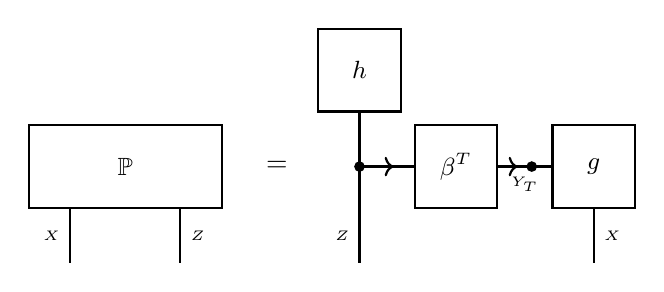
\begin{tikzpicture}[scale = 0.35, thick]

    \draw (1,-1) rectangle (8,-4);
    \node[anchor=center] (text) at (4.5,-2.5) {\corelabelsize $\probtensor$};
    \draw (2.5,-4) -- (2.5,-6) node[midway, left] {\colorlabelsize $X$};
    \draw (6.5,-4) -- (6.5,-6) node[midway, right] {\colorlabelsize $Z$};

    \node[anchor=center] (text) at (10,-2.5) {${=}$};

    \begin{scope}[shift={(15,0)}]

        \draw (-3.5,-0.5) rectangle (-0.5,2.5);
        \node[anchor=center] (text) at (-2,1) {\corelabelsize $h$};
        \draw (-2,-0.5) -- (-2,-4);
        \draw (-2,-4) -- (-2,-6) node[midway, left] {\colorlabelsize $Z$};

        \drawvariabledot{-2}{-2.5}
        \draw[] (-2,-2.5) -- (0,-2.5);
        \draw[->-] (-1.5,-2.5) -- (0,-2.5);
        \draw (0,-1) rectangle (3,-4);
        \node[anchor=center] (text) at (1.5,-2.5) {\corelabelsize $\bencodingof{T}$};

        \draw[->-] (3,-2.5) -- (4.5,-2.5);
        \drawvariabledot{4.25}{-2.5}
        \draw[] (3,-2.5) -- (5,-2.5) node[midway, below] {\colorlabelsize $\headvariableof{T}$};

        \draw (5,-1) rectangle (8,-4);
        \node[anchor=center] (text) at (6.5,-2.5) {\corelabelsize $g$};
        \draw (6.5,-4) -- (6.5,-6) node[midway, right] {\colorlabelsize $X$};
    \end{scope}
\end{tikzpicture}
    \end{center}
\end{theorem}
\begin{proof}
    Shown in more generality in the appendix, see \theref{the:generalFactorizationFisherNeyman}.
\end{proof}

%%
Notice, that the definition of sufficient statistic does not make use of the marginal distribution $\probat{\thirdcatvariable}$.
We therefore can define sufficient statistics also for families of distributions $\condprobat{\catvariable}{\thirdcatvariable}$, with respect to arbitrary non-degenerate marginal distribution $\probat{\thirdcatvariable}$.
We then use the \theref{the:factorizationFisherNeyman} to embed such families in \CompActNets{}.

\begin{corollary}
    Let $\condprobof{\shortcatvariables}{\thirdcatvariable}$ be an arbitrary family of distributions of $\shortcatvariables$, and $\sstat$ a sufficient statistic for $\thirdcatvariable$.
    Then there is a tensor $\basemeasurewith$ and a activation tensors $\acttensorat{\headvariables,\thirdcatvariable}$ such that for any $\thirdcatindex\in\mathrm{val}(\thirdcatvariable)$
    \begin{align*}
        \condprobat{\shortcatvariables}{\thirdcatvariable=\thirdcatindex} \in\cansof{\sstat,\maxgraph,\basemeasure} \, .
    \end{align*}
\end{corollary}

\begin{example}[Order Statistic for Boolean Variables: Coin toss interpretation]\label{exa:coinToss}
    Let there be $\catorder$ boolean variables $\shortcatvariables$ and a family $\{\probofat{\theta}{\shortcatvariables}\wcols\theta\in\Theta\}$ of distributions.
    The order statistic assigns to each tuple $\shortcatindices$ the ordered tuple, which effectively counts the number of $1$ coordinates in the tuple $\shortcatindices$, that is the statistic
    \begin{align*}
        \sstatof{+} \defcols \facstates \rightarrow [\seldim] \quad, \quad \sstatof{+}(\shortcatindices) = \cardof{\{\catenumerator \wcols \catindexof{\catenumerator}=1\}} \, .
    \end{align*}
    When the order statistic is sufficient, the detailed order of the outcomes is uninformative about the member $\theta\in\Theta$ from which the random variables have been drawn.
    Let us now investigate those families for which $\sstatof{+}$ is a sufficient statistic.
    By the Fisher-Neyman Factorization Theorem \theref{the:factorizationFisherNeyman} $\sstatof{+}$ is a sufficient statistic if and only if there are tensors $\basemeasurewith$ and $\acttensorat{\headvariableof{+},\Theta}$ such that for each $\theta\in\Theta$
    \begin{align*}
        \probofat{\theta}{\shortcatvariables}
        = \contractionof{
            \acttensorofat{\theta}{\headvariableof{+}},\bencodingofat{\sstatof{+}}{\headvariableof{+},\shortcatvariables},\basemeasurewith}{\shortcatvariables} \, .
    \end{align*}

    The family of distributions, such that the variables $\shortcatvariables$ are i.i.d. with respect to each (see \exaref{exa:ctHc}) are the special case, where $\basemeasurewith=\onesat{\shortcatvariables}$ and the family is labeled by $\theta\in[0,1]$ such that for $\theta\in(0,1)$ and $\catenumerator\in[\catorder+1]$
    \begin{align*}
        \acttensorofat{\theta}{\headvariableof{+}=\catenumerator}
        = (1-\theta)^{\catorder-\catenumerator} \cdot \theta^{\catenumerator} \, ,
    \end{align*}
    and for $\theta\in\{0,1\}$
    \begin{align*}
        \acttensorofat{\theta}{\headvariableof{+}}  = \begin{cases}
                                                          \onehotmapofat{0}{\headvariableof{+}} & \ifspace \theta=0 \\
                                                          \onehotmapofat{\catorder}{\headvariableof{+}} & \ifspace \theta=1
        \end{cases}\, .
    \end{align*}
    The marginal distribution $\probofat{\theta}{\headvariableof{+}}$ is then the binominal distribution $B(\catorder,\theta)$.

%    We further notce, that
%    \begin{align*}
%        \contractionof{}{}
%    \end{align*}
%    If the base measure $\basemeasurewith$ itself is elementary, we have a coin toss family, if the order statistic is sufficient for the probability.
%
%
%    For the case $\catorder=2$:
%    Consider two coin tosses \(\catvariableof{0},\catvariableof{1}\in\{0,1\}\) (1=heads). With $p \in [0,1]$ being the probability of heads. Define the statistic
%    \[
%        S(X_1,X_2)=X_1+X_2\in\{0,1,2\}.
%    \]
%    Intuitively, \(S\) forgets order and keeps only the \emph{number of heads}. The conditional law of the sequence given \(S\) is uniform over all sequences with that many heads:
%    \[
%        \mathbb{P}\!\big((X_1,X_2)=(x_1,x_2)\mid S=k\big)=\frac{1}{\binom{2}{k}}
%        \quad\text{whenever }x_1+x_2=k.
%    \]
%    Thus, knowing \(S\) renders the detailed order uninformative about the distribution—this matches the idea of a \emph{sufficient statistic}.
%
%%\end{example}
%%\begin{example}{}
%
%    % Unfair and dependent coin toss — Factorization as a \ComputationActivationNetwork{}
%    Let \(X_1,X_2\in\{0,1\}\) and define the statistic \(S(X_1,X_2)=X_1+X_2\in\{0,1,2\}\).
%    The \emph{basis (computation) core} for this statistic is
%    \[
%        \beta_S[y,x_1,x_2]\;=\;\mathbf{1}\{\,y=x_1+x_2\,\},\qquad y\in\{0,1,2\}.
%    \]
%    For $p \in (0,1)$, define a \emph{unary activation} (a vector) \(\xi[Y]\) with components \(\xi[0]=(1-p)^2,\ \xi[1]=(1-p)p,\ \xi[2]=p^2\).
%    The joint distribution factors as
%    \[
%        \mathbb{P}[X_1,X_2]\;=\;\frac{1}{Z}\,\big\langle \beta_S[Y,X_1,X_2],\,\xi[Y]\big\rangle_{Y}
%    \]
%    with
%    \begin{align*}
%        Z&\coloneqq\big\langle\,\big\langle \beta_S[Y,X_1,X_2],\,\xi[Y]\big\rangle_Y\,\big\rangle_{[\varnothing]}\\
%        &=\sum_{y=0}^{2}\xi[y]\sum_{x_1=0}^1\sum_{x_2=0}^1\beta_S[y,x_1,x_2] = 1\xi[0] + 2\xi[1] + 1\xi[2]\\
%        &= (1-p)^2+2(1-p)p+p^2 = (p+ (1-p))^2 = 1
%    \end{align*}
%    Equivalently, in coordinates,
%    \[
%        \mathbb{P}[x_1,x_2]
%        \;=\;\frac{1}{Z}\sum_{y=0}^{2}\beta_S[y,x_1,x_2]\;\xi[y]
%        \;=\;\xi\!\big(S(x_1,x_2)\big).
%    \]
%
%% \medskip
%% \noindent\emph{Numerics for \(\xi=[1,1,1]\).}
%    Since \(S(0,0)=0\), \(S(0,1)=S(1,0)=1\), and \(S(1,1)=2\),
%% the unnormalized probabilities are
%% \[
%% \mathbb{P}^\star[0,0]=1,\quad \mathbb{P}^\star[0,1]=1,\quad \mathbb{P}^\star[1,0]=1,\quad \mathbb{P}^\star[1,1]=1,
%% \]
%% hence \(Z=\sum \mathbb{P}^\star=4\) and
%% \[
%% \mathbb{P}=
%% \begin{array}{c|cc}
%%  & X_2=0 & X_2=1\\\hline
%% X_1=0 & 1/4 & 1/4\\
%% X_1=1 & 1/4 & 1/4
%% \end{array}
%% \]
%    the induced law of the statistic is
%    \[
%        \mathbb{P}[S=0]=(1-p)^2,\qquad \mathbb{P}[S=1]=2p(1-p),\qquad \mathbb{P}[S=2]=p^2,
%    \]
%    reflecting that there is only one configuration for $y \in \{0,2\}$ and 2 configurations for $ y=1$.
\end{example}

The Fisher-Neyman Theorem is the fundamental motivation for the \CompActNets{} Architecture:
\begin{itemize}
    \item The decomposition of $\acttensorwith$ is called \emph{activation network}.
    \item The decomposition of $\bencodingofat{\sstat}{\headvariables,\shortcatvariables}$ is called \emph{computation network}.
\end{itemize}

\begin{example}[Graphical Models as a special case of \CompActNets{}]
%    Recall \defref{def:compactnets}.
%    Given a statistic $\sstat:\facstates \to \parspace$ and a hypergraph $\graph=(\nodes,\edges)$ on the image coordinates $\headvariables$, any by $\sstat$ computable and by $\graph$ activated \CompActNets{} has the form
%    \begin{align*}
%        \probwith
%        = \normalizationof{\acttensorwith,\bencsstatwith}{\shortcatvariables}
%    \end{align*}
%    where $\acttensorwith$ is an arbitrary non-negative tensor.
    For graphical models we take the \emph{identity statistic}
    \begin{align*}
        \identity\big(\shortcatindices\big)
        = \shortcatindices \, ,
    \end{align*}
    so that the image coordinates coincide with the variables and there are no non-trivial computation cores.
    The associated basis encoding is just the identity tensor
    \begin{align*}
        \bencodingofat{\identity}{\headvariableof{[\catorder]},\shortcatvariables}
        = \identityat{\shortcatvariables,\headvariableof{[\catorder]}} \, .
    \end{align*}
    and therefore, for any activation tensor $\acttensorwith$ we obtain
    \begin{align*}
        \probwith
        &= \normalizationof{\acttensorwith,\bencodingofat{\identity}{\headvariableof{[\catorder]},\shortcatvariables}}{\shortcatvariables}
        & = \normalizationof{\acttensorat{\shortcatvariables}}{\shortcatvariables}
    \end{align*}
    In other words, in the graphical–model case the activation tensor coincides with the joint distribution tensor.
    In this setting, structural properties of the distribution such as (conditional) independences can be read off as algebraic factorization patterns of the activation (and hence joint) tensor.
\end{example}

\subsection{Exponential families in case of elementary activation tensors}

% Universal properties
A classical theorem by Pitman-Koopman-Darmois (see \cite{pitman_sufficient_1936}) states, that whenever a family with constant support and a finite sufficient statistic for arbitrary large data sets is in an exponential family.
We now restrict the activation cores to specific elementary tensors, which correspond with further assumptions on the dependence of $\probtensor$ and $\sstat$ made by exponential families.
For a discussion of further universal properties of exponential families, such that the existence of priors and entropy maximizers, see \cite{murphy_probabilistic_2022}.

\begin{definition}[Exponential Family]
    %\alex{was \theref{the:expFamilyTensorRep}}
    Given a base measure $\basemeasure$ and a statistic $\sstat:\facstates\rightarrow\parspace$ we enumerate for each coordinate $\selindexin$ the image $\imageof{\sstatcoordinateof{\selindex}}$ by an interpretation map
    \begin{align*}
        \indexinterpretationof{\selindex} \defcols
        [\cardof{\imageof{\sstatcoordinateof{\selindex}}}] \rightarrow \imageof{\sstatcoordinateof{\selindex}} \, .
    \end{align*}
    For any canonical parameter vector $\canparamwithin$ we build the activation cores $\softactlegwith$ for each coordinate $\headindexof{\selindex}\in[\cardof{\imageof{\sstatcoordinateof{\selindex}}}]$ by
    \begin{align*}
        \softactlegat{\indexedheadvariableof{\selindex}}
        = \expof{\canparamat{\indexedselvariable} \cdot \indexinterpretationofat{\selindex}{\headindexof{\selindex}}} \,
    \end{align*}
    and define the distribution % Could do parametrization to thirdcatvariable to make connection with the family definition..
    \begin{align*}
        \expdistwith =
        \normalizationof{\{\basemeasurewith\} \cup \{\bencodingofat{\sstatcoordinateof{\selindex}}{\headvariableof{\selindex},\shortcatvariables} \wcols \selindexin\}\cup\{\softactlegwith \wcols \selindexin\}}{\shortcatvariables} \, .
    \end{align*}
    We then call the tensor $\probfamilyofat{\sstat,\basemeasure}{\shortcatvariables}{\Theta}$ with $\valof{\Theta}=\parspace$ and slices for $\canparamin$ by
    \begin{align*}
        \probfamilyofat{\sstat,\basemeasure}{\shortcatvariables}{\Theta=\canparam}
        = \expdistwith
    \end{align*}
    the exponential family to the statistic $\sstat$ and the base measure $\basemeasure$.
\end{definition}

%% In Elementary Activations
Note that by construction each member of an exponential family is an element in a \CompActNet{} with elementary activation cores, that is
\begin{align*}
    \probfamilyofat{\sstat,\basemeasure}{\shortcatvariables}{\Theta=\canparam}
    \in \cansof{\sstat,\elgraph,\basemeasure} \, .
\end{align*}

\begin{figure}
    \begin{center}
        \input{../tikz_pics/probability_representation/expdist_elementary}
    \end{center}
    \caption{
        Tensor Network diagram of a member of an exponential family $\probfamilyofat{\sstat,\basemeasure}{\shortcatvariables}{\Theta=\canparam}$ before normalization as an \CompActNet{} with elementary activation, that is an element in $\cansof{\sstat,\elgraph,\basemeasure}$.}\label{fig:expdistElementary}
\end{figure}

%% NEEDED?
\begin{example}[Joint distributions of two booleans]
%{\alex{Joint distributions of two Booleans, sufficient statistic by head count (coin toss interpretation) and exponential family in case of independence}}
    In general, joint distribution of two Boolean variables $\catvariableof{0},\catvariableof{1}$ are 2x2 matrices of non-negative coordinates summing to 1:
    \[
        \probat{\catvariableof{[2]}}= \begin{bmatrix}
                                  p_{0,0} & p_{0,1} \\
                                  p_{1,0} & p_{1,1}
        \end{bmatrix}
    \]
    In the following example, we will assume at different points that $\catvariableof{0},\catvariableof{1}$ have a sufficient statistic, are independent and they have positive distributions.
    By the normalization constraint, $p_{1,1}$ is determined from $p_{0,0},p_{0,1}$ and $p_{1,0}$, which leaves us with three free parameters.
    \[
        \probat{\catvariableof{[2]}}= \begin{bmatrix}
                                  p_{0,0} & p_{0,1} \\
                                  p_{1,0} & 1-(p_{0,0}+p_{0,1}+p_{1,0})
        \end{bmatrix}
    \]

    Let us now restrict to those distributions, which have the sum $\catvariableof{0}+\catvariableof{1}$ as a sufficient statistic.
    They need to satisfy $p_{0,1}=p_{1,0}$ (since in that cases the statistic is 1 and the definition of sufficiency is that the distribution conditioned on the statistic is uniform), leaving us with two free parameters.
    \[
        \probat{\catvariableof{[2]}}= \begin{bmatrix}
                                  p_{0,0} & p_{0,1} \\
                                  p_{0,1} & 1-p_{0,0}-2p_{0,1}
        \end{bmatrix}
    \]
    This symmetry also implies, that the distributions are identically distributed, i.e. for any $\catindex\in\{0,1\}$ we have % with $\mathbb{I}_2 = (1,1)^\intercal$:
    \begin{align*}
        \probat{\catvariableof{0}=\catindex}
        = \contractionof{\probat{\catvariableof{0},\catvariableof{1}}}{\catvariableof{0}=\catindex}
        = \contractionof{\probat{\catvariableof{1},\catvariableof{0}}}{\catvariableof{1}=\catindex}
        = \probat{\catvariableof{1}=\catindex} \, .
    \end{align*}
%    \[
%        \probat{\catvariableof{0}}
%        = \left\langle \probat{\catvariableof{0},\catvariableof{1}}, \mathbb{I}[\catvariableof{1}] \right\rangle[\catvariableof{0}] = \probat{\catvariableof{0},\catvariableof{1}}\mathbb{I}_2 = \probat{\catvariableof{1},\catvariableof{0}} \mathbb{I}_2 = \left\langle \probat{\catvariableof{0},\catvariableof{1}}, \mathbb{I}[\catvariableof{0}] \right\rangle[\catvariableof{1}]
%        =\probat{\catvariableof{1}}.
%    \]

    Restricting further to those, where $\catvariableof{0}$ and $\catvariableof{1}$ are independent and the distribution is everywhere supported, brings us to the rank one formulation of the distribution
    \[
        \probat{\catvariableof{0},\catvariableof{1}} = \begin{bmatrix}
                               \probat{\catvariableof{0}=0}\probat{\catvariableof{1}=0} & \probat{\catvariableof{0}=0}\probat{\catvariableof{1}=1}\\
                               \probat{\catvariableof{0}=1}\probat{\catvariableof{1}=0} & \probat{\catvariableof{0}=1}\probat{\catvariableof{1}=1}
        \end{bmatrix} = \probat{\catvariableof{0}} \otimes \probat{\catvariableof{1}} %= \probat{\catvariableof{0}}\probat{\catvariableof{0}}^\intercal.
    \]
    In terms of an exponential family with the head count as a sufficient statistic, we parametrize the distribution by the canonical parameter $\canparam\in\rr$ as
    \[
        \probat{\catvariableof{0}}
        =\frac{1}{1+\expof{\canparam}}
        \begin{bmatrix}
            1 \\
            \expof{\canparam}
        \end{bmatrix}
    \]
    Note, that with this parametrization the probabilities for head and tail automatically have the form $p, (1-p)$.
    \[
        % \frac{1}{1+2\cdot\expof{\canparam}+\expof{2\canparam}}
        %     \begin{bmatrix}
        %         1 & \expof{\canparam} \\
        %         \expof{\canparam} & \expof{2\canparam}
        %     \end{bmatrix}
        % =
        \probat{\catvariableof{0},\catvariableof{1}} = \frac{1}{(1+\expof{\canparam})^2} \begin{bmatrix}
                                                                 1 \\
                                                                 \expof{\canparam}
        \end{bmatrix}
        \begin{bmatrix}
            1 &  \expof{\canparam}
        \end{bmatrix}
    \]
    % Furthermore, from the decomposition on the right side we see that $\catvariableof{0}$ and $\catvariableof{1}$ are independent.
    % Conversely, if $\catvariableof{0}$ and $\catvariableof{1}$ are independent and the distribution has the head count as sufficient statistic, $\catvariableof{0}$ and $\catvariableof{1}$ need to also be identical distributed (otherwise we would have $p_{0,1}\neq p_{1,0}$).
    % Using that the support is maximal, we find a $\canparam\in\rr$ such that 


    % and their joint distribution is the member of the exponential family to this parameter $\canparam$.

    %% SEE EXAMPLE 5.5 in [Lehmann Casella - Theory of Point Estimation]
    We can interpret this distribution as two independent coin tosses with outcome $\catvariableof{0}$ and $\catvariableof{1}$ and head probability
    \begin{align*}
        \probat{\catvariableof{0}=1} = \probat{\catvariableof{1}=1} = \frac{\expof{\canparam}}{1+\expof{\canparam}}
    \end{align*}
    which is the sigmoid of $\canparam$ and inverted by the logit
    \begin{align*}
        \canparam = \lnof{\frac{\probat{\catvariableof{0}=1}}{1-\probat{\catvariableof{0}=1}}} \, .
    \end{align*}
    Consistent with the above parametrization, we have a uniform distribution of $\catvariableof{0}$ and $\catvariableof{1}$ in the fair coin toss case $\probat{\catvariableof{0}=1}=0.5$, where $\canparam=0$.

    As a \ComputationActivationNetwork{} we can represent any distribution $\probat{\catvariableof{0},\catvariableof{1}}$ with the head count $+$ as sufficient statistic by
    \begin{align*}
        \probat{\catvariableof{0},\catvariableof{1}}
        &= \normalizationof{\bencodingofat{+}{\headvariableof{+},\catvariableof{0},\catvariableof{1}},\acttensorat{\headvariableof{+}}}{\catvariableof{0},\catvariableof{1}} \, ,
    \end{align*}
    such that
    \begin{align*}
        \probat{\indexedcatvariableof{0},\indexedcatvariableof{1}}
        &= \frac{1}{Z}\contractionof{\bencodingofat{+}{\headvariableof{+},\catvariableof{0},\catvariableof{1}},\acttensorat{\headvariableof{+}}}{\indexedcatvariableof{0},\indexedcatvariableof{1}}\\
        &=\frac{1}{Z}\sum_{\headindexof{+}\in[2]}
        \bencodingofat{+}{\indexedheadvariableof{+},\indexedcatvariableof{0},\indexedcatvariableof{1}} \cdot \acttensorat{\indexedheadvariableof{+}} \\
        & = \frac{1}{Z} \acttensorat{\headvariableof{+}=\catindexof{0}+\catindexof{1}} \, ,
    \end{align*}
    where the normalization constant $Z$ cancels out any multiplicative constant $\lambda\in\mathbb{R}\backslash\{0\}$ in $\xi$ and the equation above implies
    \begin{align*}
        \acttensorat{\headvariable} = \lambda \cdot
        \begin{bmatrix}
            p_{0,0} \\
            p_{0,1} \\
            p_{1,1}
        \end{bmatrix} \, .
    \end{align*}
    We choose $\lambda=1/p_{0,0} = (1+\exp[\theta])^2$ in the following.
    Among these distribution, the exponential family with the head count statistic is then parametrized by activation tensors
    \begin{align*}
        \acttensorat{\headvariable} = \begin{bmatrix}
                                          1\\
                                          p_{0,1}/p_{0,0}\\
                                          p_{1,1}/p_{0,0}
        \end{bmatrix}
        =
        \begin{bmatrix}
            1 \\
            \expof{\canparam} \\
            \expof{2\canparam}
        \end{bmatrix} \, ,
    \end{align*}
    since $p_{0,1} = \probat{\catvariableof{0}=0}\cdot\probat{\catvariableof{0}=1} = (1+\exp[\theta])^{-1}\cdot\exp[\theta](1+\exp[\theta])^{-1}$ and $p_{1,1} = (\exp[\theta](1+\exp[\theta])^{-1})^2$.
\end{example}


\subsection{Efficient Contractions by Message Passing}

\alex{Contractions of tensor networks are generally hard to solve.
We here investigate message passing algorithms, which decompose contractions into a sequence of subcontractions, which are passed as messages through the tensor network.}
The resulting algorithm is called Belief Propagation \algoref{alg:treeBeliefPropagation}.
We denote $\dirovedges$ to be all tuples $(\sedge,\redge)$ of hyperedges $\sedge,\redge\in\edges$ such that $\sedge\neq\redge$ and $\sedge\cap\redge\neq\varnothing$.

%\begin{algorithm}[hbt!]
%    \caption{Belief Propagation}\label{alg:treeBeliefPropagation}
%    \begin{algorithmic}
%        \Require Tensor network $\extnet$ on a hypergraph $\graph$
%        \Ensure Messages $\{\messagewith\wcols(\secsedge,\sedge)\in\dirovedges\}$
%        \iosepline
%        \State Initialize $\scheduler$ (differs in implementation)
%        \State Initialize messages
%        \While{$\scheduler$ not empty}
%            \State Take a $(\sedge,\redge)$ pair from $\scheduler$
%            \State Update the message
%            \begin{align*}
%                \messagewith
%                = \contractionof{\{\hypercoreofat{\sedge}{\catvariableof{\sedge}}\}
%                    \cup \{\mesfromtoat{\secsedge}{\sedge}{\catvariableof{\secsedge\cap\sedge}} \wcols (\secsedge,\sedge)\in\dirovedges \ncond \secsedge\neq \redge\}
%                }{\catvariableof{\sedge\cap \redge}}
%            \end{align*}
%            \State Update $\scheduler$ (differs in implementation)
%        \EndWhile
%        \State \Return Messages $\{\messagewith\wcols(\secsedge,\sedge)\in\dirovedges\}$
%    \end{algorithmic}
%\end{algorithm}

\begin{algorithm}[hbt!]
    \caption{Tree Belief Propagation}\label{alg:treeBeliefPropagation}
    \begin{algorithmic}
        \Require Tensor network $\extnet$ on a hypergraph $\graph$
        \Ensure Messages $\{\messagewith\wcols(\secsedge,\sedge)\in\dirovedges\}$
        \iosepline
        \State Initialize $\scheduler=\{(\secsedge,\sedge) \wcols \secsedge \quad\text{a leaf in } \graph \}]$
%        \State Initialize empty
        \While{$\scheduler$ not empty}
            \State Pop a $(\sedge,\redge)$ pair from $\scheduler$
            \State Compute the message
            \begin{align*}
                \messagewith
                = \contractionof{\{\hypercoreofat{\sedge}{\catvariableof{\sedge}}\}
                    \cup \{\mesfromtoat{\secsedge}{\sedge}{\catvariableof{\secsedge\cap\sedge}} \wcols (\secsedge,\sedge)\in\dirovedges \ncond \secsedge\neq \redge\}
                }{\catvariableof{\sedge\cap \redge}}
            \end{align*}
            \State Update $\scheduler$ by all messages $(\redge,\thirdsedge)$ which have not yet been sent, if all messages $(\secsedge,\redge)$ to $\secsedge\neq\thirdsedge$ have been sent.
        \EndWhile
        \State \Return Messages $\{\messagewith\wcols(\secsedge,\sedge)\in\dirovedges\}$
    \end{algorithmic}
\end{algorithm}

\begin{theorem}
    \label{the:treeBeliefPropagationExactness}
    The messages in the tree belief propagation are contracted to local marginals, that is for each $\sedge\in\edges$ we have
    \begin{align*}
        \contractionof{\extnet}{\catvariableof{\sedge}}
        \contractionof{\{\hypercoreofat{\sedge}{\catvariableof{\sedge}}\}\cup
            \{\mesfromtowith{\secsedge}{\sedge} \wcols (\secsedge,\sedge)\in\dirovedges\}}{\catvariableof{\edge}} \, .
    \end{align*}
\end{theorem}

We show \theref{the:treeBeliefPropagationExactness} based on the following lemma.
We denote for each pair $(\sedge,\redge)$ the subset $\preedgeset\subset\edges$ as the subset of edges $\edgein$, for which each path to $\redge$ passes through $\sedge$.
Note, that by construction $\sedge\in\preedgeset$.

\begin{lemma}
    \label{lem:messageAsContraction}
    For any tensor network on a tree hypergraph, \algoref{alg:contractionPropagation} terminates in the tree-based implementation and returns final messages
    \begin{align*}
        \messagewith
        = \contractionof{\{\edgehypercorewith\wcols\edge\in\preedgeset\}}{\catvariableof{\sedge\cap\redge}}
    \end{align*}
\end{lemma}
\begin{proof}
    We show this property by induction over the edge sets $\preedgeset$ to pairs $(\sedge,\redge)\in\dirovedges$, such that $\cardof{\preedgeset}\leq n$.
    Notice, that since always $\sedge\in\preedgeset$ we have $n\geq1$.

    $n=1$: In this case we have $\preedgeset=\{\sedge\}$ and $\sedge$ is a leaf of the tree-hypergraph $\graph$.
    The claimed message property holds thus by definition.

    $n\rightarrow n+1$: Let us assume, that the message obeys the claimed property for edge sets with cardinality up to $n$.
    If there is no edge set with cardinality $n+1$, the property holds also for those with cardinality up to $n+1$.
    If there is an edge set $\preedgeset$ with size $n+1$, we have
    \begin{align*}
        \preedgeset = \{\sedge\} \cup \left(\bigcup_{\secsedge \in\dirovedges} \preedgesetwrt{\secsedge}{\sedge}\right) \, .
    \end{align*}
    The message $\mesfromto{\sedge}{\redge}$ is sent, once all messages $\mesfromto{\secsedge}{\sedge}$ to $(\secsedge,\sedge)\in\dirovedges\{(\redge,\sedge)\}$ arrived.
    By definition we have
    \begin{align*}
        \mesfromtowith{\sedge}{\redge}%{\catvariableof{\sedge\cap \redge}}
        = \contractionof{\{\hypercoreofat{\sedge}{\catvariableof{\sedge}}\}
            \cup \{\mesfromtowith{\secsedge}{\sedge} \wcols (\secsedge,\sedge) \in\dirovedges \ncond \secsedge \neq \redge \}
        }{\catvariableof{\sedge\cap \redge}}
    \end{align*}
    Now we use the induction assumption on $\preedgesetwrt{\secsedge}{\sedge}$ (since its cardinality is at most $n$) and get
    \begin{align*}
        \mesfromtoat{\sedge}{\redge}{\catvariableof{\sedge\cap \redge}}
        &= \contractionof{
            \{\hypercoreofat{\sedge}{\catvariableof{\sedge}}\} \cup
            \left(\bigcup_{(\secsedge,\sedge)\in\dirovedges \ncond \secsedge\neq \redge}
                \contractionof{\{\hypercoreofat{\thirdsedge}{\catvariableof{\thirdsedge}} \wcols  \thirdsedge \in \preedgesetwrt{\secsedge}{\sedge}\}}{\catvariableof{\secsedge\cap \sedge}} \right)
        }{\catvariableof{\sedge\cap \redge}} \\
        &= \contractionof{
            \{\hypercoreofat{\sedge}{\catvariableof{\sedge}}\} \cup
            \left(\bigcup_{(\secsedge,\sedge)\in\dirovedges \ncond \secsedge\neq \redge} \{\hypercoreofat{\thirdsedge}{\catvariableof{\thirdsedge}} \wcols  \thirdsedge \in \preedgesetwrt{\secsedge}{\sedge}\} \right)
        }{\catvariableof{\sedge\cap \redge}} \\
        &= \contractionof{\{\edgehypercorewith\wcols\edge\in\preedgeset\}}{\catvariableof{\sedge\cap\redge}}
    \end{align*}
    Here we used the commutation of contraction property in the second equation, which is justified by the assumed tree property of the hypergraph.
    Thus, the message property holds also for any edge sets of size $n+1$.

    By induction, the claimed message property therefore holds for all final messages.
\end{proof}

\begin{proof}[Proof of \theref{the:treeBeliefPropagationExactness}]
    Since the hypergraph is by assumption a tree, we can partition $\edges$ into disjoint subsets $\{\sedge\}$ and $\preedgesetwrt{\secsedge}{\sedge}$ for $(\secsedge,\sedge)\in\dirovedges$.
    We then have
    \begin{align*}
        \contractionof{\extnet}{\catvariableof{\sedge}}
        =& \contractionof{\{\hypercoreofat{\sedge}{\catvariableof{\sedge}}\}
            \cup \left\{\contractionof{\hypercoreofat{\edge}{\catvariableof{\edge}}\wcols\edge\in\preedgesetwrt{\secsedge}{\sedge}}{\catvariableof{\edge\cap\secsedge}} \wcols (\secsedge,\sedge)\in\dirovedges \right\}
        }{\catvariableof{\sedge}} \\
        =& \contractionof{\{\hypercoreofat{\sedge}{\catvariableof{\sedge}}\} \cup \{\mesfromtowith{\secsedge}{\sedge} \wcols (\secsedge,\sedge)\in\dirovedges\}}{\catvariableof{\sedge}} \, .
    \end{align*}
    Here we used \lemref{lem:messageAsContraction} in the second equation.
\end{proof}

% Example by Student Markov Network
We examplify the usage of \algoref{alg:treeBeliefPropagation} on the Markov Network of \exaref{exa:studentHC}.

\begin{example}[Continuation of \exaref{exa:studentHC}]
    \label{exa:studentBP}
    We exemplify the Belief Propagation \algoref{alg:treeBeliefPropagation} on the Markov network in the student example (see \exaref{exa:studentHC}).
    The directions of the messages result from the hyperedge overlaps (see \figref{fig:studentMessagePassingDirections} a) and the resulting directions $\dirovedges$ are sketched in \figref{fig:studentMessagePassingDirections} b).
    The messages to $\{(\edgeof{2},\edgeof{0}),(\edgeof{0},\edgeof{2})\}$ are vectors of $\catvariableof{G}$ and the messages $\{(\edgeof{0},\edgeof{1}),(\edgeof{1},\edgeof{0})\}$ are vectors of $\catvariableof{I}$.

    Since the hyperedges are minimally connected, we can implement \algoref{alg:treeBeliefPropagation} by a tree scheduler $\scheduler$:
    \begin{itemize}
        \item The scheduler is initialized with messages from leafs, in our example $\{(\edgeof{2},\edgeof{0}),(\edgeof{1},\edgeof{0})\}$.
        \item Each message is placed exactly once on $\scheduler$, when at a hyperedge all but the reverse message have been received.
        In our example, after execution of $(\edgeof{2},\edgeof{0})$ the message $(\edgeof{0},\edgeof{1})$ is placed on $\scheduler$ and after execution of $(\edgeof{1},\edgeof{0})$ the message $(\edgeof{0},\edgeof{2})$.
    \end{itemize}
    In this implementation, \algoref{alg:treeBeliefPropagation} terminates after $\cardof{\dirovedges}=4$ iterations of the \whileSymbol{} loop.
    The exact marginals of the edge variables are then
    \begin{align*}
        \probat{\catvariableof{L},\catvariableof{G}}
        &= \normalizationof{
            \hypercoreofat{\edgeof{2}}{\catvariableof{L},\catvariableof{G}},
            \mesfromto{\edgeof{0}}{\edgeof{2}}\left[\catvariableof{G}\right]
        }{\catvariableof{L},\catvariableof{G}}, \\
        \probat{\catvariableof{G},\catvariableof{D},\catvariableof{I}}
        &= \normalizationof{\hypercoreofat{\edgeof{0}}{\catvariableof{G},\catvariableof{D},\catvariableof{I}},
            \mesfromto{\edgeof{2}}{\edgeof{0}}\left[\catvariableof{G}\right],
            \mesfromto{\edgeof{1}}{\edgeof{0}}\left[\catvariableof{I}\right]
        }{\catvariableof{G},\catvariableof{D},\catvariableof{I}}, \\
        \probat{\catvariableof{I},\catvariableof{S}}
        &= \normalizationof{
            \hypercoreofat{\edgeof{1}}{\catvariableof{I},\catvariableof{S}},
            \mesfromto{\edgeof{0}}{\edgeof{1}}\left[\catvariableof{I}\right]
        }{\catvariableof{I},\catvariableof{S}} \, .
    \end{align*}

\end{example}


\begin{figure}[t]
    \begin{center}
        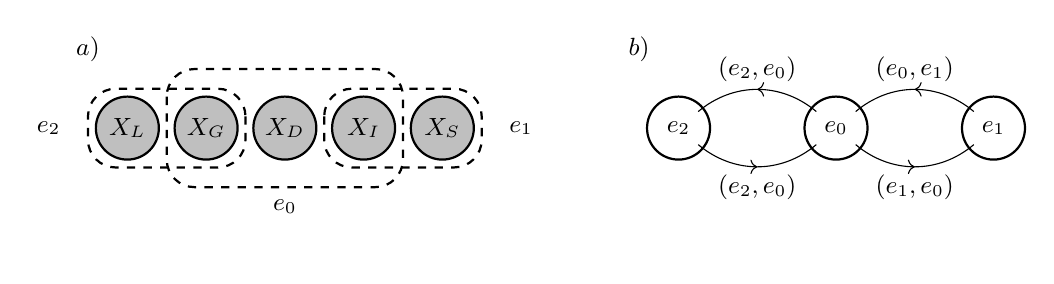
\begin{tikzpicture}
            \node[anchor=center] (A) at (-0.5,3) {\corelabelsize $a)$};

            \node[circle, draw, thick, fill=\nodegrayscale, minimum size = \nodeminsize] (A) at (0,2) {};
            \node[anchor=center] (A) at (0,2) {\corelabelsize $\catvariableof{L}$};
            \node[circle, draw, thick, fill=\nodegrayscale, minimum size = \nodeminsize] (A) at (1,2) {};
            \node[anchor=center] (A) at (1,2) {\corelabelsize $\catvariableof{G}$};
            \node[circle, draw, thick, fill=\nodegrayscale, minimum size = \nodeminsize] (A) at (2,2) {};
            \node[anchor=center] (A) at (2,2) {\corelabelsize $\catvariableof{D}$};
            \node[circle, draw, thick, fill=\nodegrayscale, minimum size = \nodeminsize] (A) at (3,2) {};
            \node[anchor=center] (A) at (3,2) {\corelabelsize $\catvariableof{I}$};
            \node[circle, draw, thick, fill=\nodegrayscale, minimum size = \nodeminsize] (A) at (4,2) {};
            \node[anchor=center] (A) at (4,2) {\corelabelsize $\catvariableof{S}$};

            \node (of) at (0,0.5) {};
            \draw[thick, dashed, rounded corners=10pt]  ($(1.5,2)+(of)$) -- ($(1.5,2)-(of)$)  -- ($(-0.5,2)-(of)$) -- ($(-0.5,2)+(of)$) -- cycle;
            \node[anchor=center] (A) at (-1,2) {\corelabelsize $\edgeof{2}$};

            \draw[thick, dashed, rounded corners=10pt]  ($(2.5,2)+(of)$) -- ($(2.5,2)-(of)$)  -- ($(4.5,2)-(of)$) -- ($(4.5,2)+(of)$) -- cycle;
            \node[anchor=center] (A) at (5,2) {\corelabelsize $\edgeof{1}$};
            \node (of) at (0,0.75) {};
            \draw[thick, dashed, rounded corners=10pt]  ($(0.5,2)+(of)$) -- ($(0.5,2)-(of)$)  -- ($(3.5,2)-(of)$) -- ($(3.5,2)+(of)$) -- cycle;
            \node[anchor=center] (A) at (2,1) {\corelabelsize $\edgeof{0}$};

            \begin{scope}[shift={(7,0)}]
                \node[anchor=center] (A) at (-0.5,3) {\corelabelsize $b)$};

                \node[circle, draw, thick, minimum size = \nodeminsize] (A) at (0,2) {};
                \node[anchor=center] (E0) at (0,2) {\corelabelsize $\edgeof{2}$};

                \node[circle, draw, thick, minimum size = \nodeminsize] (A) at (2,2) {};
                \node[anchor=center] (E1) at (2,2) {\corelabelsize $\edgeof{0}$};

                \node[circle, draw, thick, fill=white, minimum size = \nodeminsize] (A) at (4,2) {};
                \node[anchor=center] (E2) at (4,2) {\corelabelsize $\edgeof{1}$};

                \draw[->-] (E0) to[bend right = 40] (E1);
                \node[anchor=center] at (1,2.75) {\corelabelsize $(\edgeof{2},\edgeof{0})$};
                \draw[->-] (E1) to[bend right = 40] (E0);
                \node[anchor=center] at (1,1.25) {\corelabelsize $(\edgeof{2},\edgeof{0})$};
                \draw[->-] (E1) to[bend right = 40] (E2);
                \node[anchor=center] at (3,2.75) {\corelabelsize $(\edgeof{0},\edgeof{1})$};
                \draw[->-] (E2) to[bend right = 40] (E1);
                \node[anchor=center] at (3,1.25) {\corelabelsize $(\edgeof{1},\edgeof{0})$};
            \end{scope}
        \end{tikzpicture}
    \end{center}
    \caption{a) Sketch of the overlap of the edges, resulting in the message directions b) $\dirovedges=\{(\edgeof{2},\edgeof{0}),(\edgeof{0},\edgeof{2}),(\edgeof{0},\edgeof{1}),(\edgeof{1},\edgeof{0})\}$.}\label{fig:studentMessagePassingDirections}
\end{figure}
\section{The Neural Paradigm}

The neural paradigm of artificial intelligence exploits the decomposition of functions into neurons, which are aligned in a directed acyclic graph.
We show in this section how functions decomposeable into neurons can be represented by tensor networks.
To this end we formalize discrete neural models in decomposition graphs and formally proof the corresponding decomposition of their basis encodings.
Particular examples will be presented in the next section by propositional formulas with sparse syntactical descriptions.

\subsection{Function Decomposition}

\begin{lemma}
    \label{lem:formulaDecomp}
    Let $\formulaat{\shortcatvariables}$ be a composition of a $\seldim$-ary connective function $\exconnective$ and functions $\formulaofat{\selindex}{\shortcatvariables}$, where $\selindexin$, i.e. for $\shortcatindices\in\atomstates$ we have
    \begin{align*}
        \formulaat{\indexedshortcatvariables}
        = \exconnective\left(\formulaofat{0}{\indexedshortcatvariables}, \dots, \formulaofat{\seldim-1}{\indexedshortcatvariables}\right) \, .
    \end{align*}
    Then we have
    \begin{align*}
        \bencodingofat{\formula}{\headvariableof{\formula},\shortcatvariables}
        = \contractionof{
            \{\bencodingofat{\exconnective}{\headvariableof{\formula},\headvariableof{[\seldim]}}\}
            \cup \{\bencodingofat{\formulaof{\selindex}}{\headvariableof{\selindex},\shortcatvariables} \wcols \selindexin\}
        }{\headvariableof{\formula},\shortcatvariables} \, .
    \end{align*}
\end{lemma}
\begin{proof}
    This can be shown on each index $\shortcatindices$.
\end{proof}

For the composition of two functions $\formulaat{\shortcatvariables}$ and $\secexformula\left[\shortcatvariables\right]$ the composition by some binary connective is pictured by:
\begin{center}
    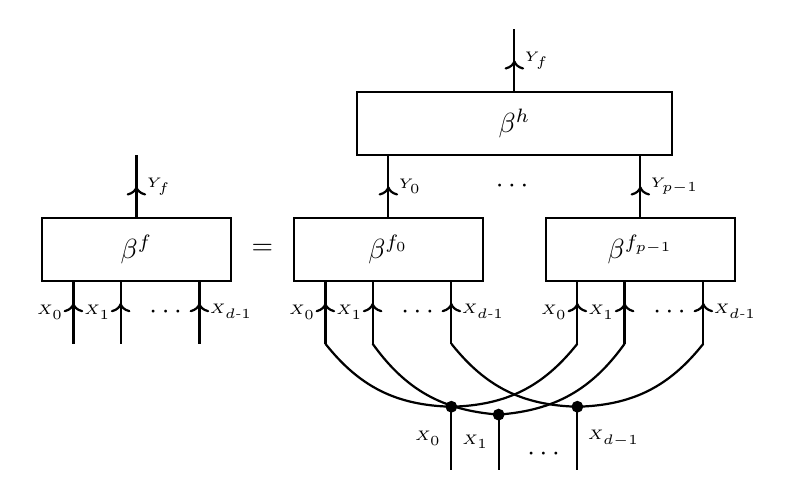
\begin{tikzpicture}[scale=0.4, thick]
    \begin{scope}

        % \node[anchor=center] (text) at (-6,-4) {$b)$};

        \begin{scope}
        [shift={(-8,0)}]
            \draw[->-] (5.5,-9)--(5.5,-7) node[midway,right] {\colorlabelsize $\headvariableof{\exformula}$};
            \drawatomcore{3.5}{-8}{$\bencodingof{\exformula}$}
            \drawatomindices{3.5}{-12}
        \end{scope}

        \node[anchor=center] (text) at (1.5,-10) {${=}$};

        \draw[->-] (9.5,-5)--(9.5,-3) node[midway,right] {\colorlabelsize $\headvariableof{\exformula}$};

        \node[anchor=center] (text) at (9.5,-6) {$\bencodingof{\chainingfunction}$};
        \draw (4.5,-7) rectangle (14.5,-5);

        \draw[->-] (5.5,-9)--(5.5,-7) node[midway,right] {\colorlabelsize $\headvariableof{0}$};

        \node[anchor=center] at (9.5,-8) {$\cdots$};

        \drawatomcore{3.5}{-8}{$\bencodingof{\formulaof{0}}$}
        \drawatomindices{3.5}{-12}

        \begin{scope}
        [shift={(8,0)}]

            \draw[->-] (5.5,-9)--(5.5,-7) node[midway,right] {\colorlabelsize $\headvariableof{\seldim-1}$};

            \drawatomcore{3.5}{-8}{$\bencodingof{\formulaof{\seldim-1}}$}
            \drawatomindices{3.5}{-12}

        \end{scope}

        \draw[fill] (7.5,-15) circle (\dotsize);
        \draw[] (7.5,-15) to[bend left=25] (3.5,-13);
        \draw[] (7.5,-15) to[bend right=25] (11.5,-13);

        \draw[fill] (9,-15.25) circle (\dotsize);
        \draw[] (9,-15.25) to[bend left=25] (5,-13);
        \draw[] (9,-15.25) to[bend right=25] (13,-13);

        \draw[fill] (11.5,-15) circle (\dotsize);
        \draw[] (11.5,-15) to[bend left=25] (7.5,-13);
        \draw[] (11.5,-15) to[bend right=25] (15.5,-13);



        \draw[] (7.5,-15)--(7.5,-17) node[midway,left] {\colorlabelsize $\catvariableof{0}$};
        \draw[] (9,-15.25)--(9,-17) node[midway,left] {\colorlabelsize $\catvariableof{1}$};
        \node[anchor=center] (text) at (10.5,-16.5) {$\cdots$};
        \draw[] (11.5,-15)--(11.5,-17) node[midway,right] {\colorlabelsize $\catvariableof{\atomorder-1}$};

    \end{scope}
\end{tikzpicture}
\end{center}

Let us now define a more generic decomposition of discrete functions.

\begin{definition}
    \label{def:decompositionHypergraph}
    A decomposition hypergraph is a directed acyclic hypergraph $\graph=(\nodes,\edges)$ such that
    \begin{itemize}
        \item Each node $\nodein$ is decorated by a set $\arbsetof{\node}$ of finite cardinality $\catdimof{\node}$, a variable $\catvariableof{\node}$ and an index interpretation function
        \begin{align*}
            \indexinterpretationof{\node} \defcols [\catdimof{\node}] \rightarrow \arbsetof{\node} \, .
        \end{align*}
        \item Each directed hyperedge $(\incomingnodes,\outgoingnodes)$ has at least one outgoing node, i.e. $\outgoingnodes\neq\varnothing$ and is decorated by an activation function % propositional formula
        \begin{align*}
            \secexfunctionof{\node} \defcols
            \bigtimes_{\node\in\incomingnodes} \arbsetof{\node}
            \rightarrow \bigtimes_{\node\in\outgoingnodes} \arbsetof{\node} \, .
        \end{align*}
        \item Each node $\nodein$ appears at most once as an outgoing node. % Well-defined function
        \item The nodes not appearing as an outgoing node are enumerated by $\node^{\insymbol}_{[\atomorder]}$.
        We abbreviate the corresponding variables by $\catvariableof{\node^{\insymbol}_{[\atomorder]}}=\shortcatvariables$. % and labeled by $\nodes^{\insymbol}_{[\atomorder]}$.
        \item The nodes not appearing as an incoming node are enumerated by $\node^{\outsymbol}_{[\seldim]}$.
        We abbreviate the variables by $\catvariableof{\node^{\outsymbol}_{[\selindex]}},\catvariableof{\node^{\insymbol}_{[\atomorder]}}=\headvariables$. %$[\seldim]$ are labeled by $\nodes^{\outsymbol}_{[\seldim]}$.
    \end{itemize}
    We assign for each $\catenumeratorin$ restriction functions
    \begin{align*}
        \restrictionofto{\cdot}{\node^{\insymbol}_\catenumerator}
        \defcols \bigtimes_{\seccatenumerator\in[\catorder]} \arbsetof{\node^{\insymbol}_{\seccatenumerator}} \rightarrow \arbsetof{\node^{\insymbol}_\catenumerator}
        \quad,\quad  \restrictionofto{\catindexof{[\catorder]}}{\catenumerator} = \catindexof{\catenumerator}
    \end{align*}
    to the nodes $\node^{\insymbol}_{[\atomorder]}$ and recursively assign to each further node $\node$ a node function % connective $\connectiveofat{\node}{\headvariableof{\incomingnodes}}$.
    \begin{align*}
        \exfunctionof{\node} \wcols \bigtimes_{\catenumeratorin} \arbsetof{\node^{\insymbol}_\catenumerator} \rightarrow \bigtimes_{\node\in\outgoingnodes} \arbsetof{\node}
        \quad,\quad
        \exfunctionof{\node}(\catindexof{[\catorder]})
        = \secexfunctionof{\node}\left(\bigtimes_{\node\in\incomingnodes}\restrictionofto{\exfunctionof{\edgeof{\node}}(\catindexof{[\catorder]})}{\node}\right) \, ,
    \end{align*}
    where $\edgeof{\node}$ is to each $\node\in\incomingnodes$ the unique hyperedge with outgoing nodes $\{\node\}$.
    We then call the function
    \begin{align*}
        \exfunctionof{\graph} \wcols \bigtimes_{\catenumeratorin} \arbsetof{\node^{\insymbol}_\catenumerator} \rightarrow \bigtimes_{\selindexin} \arbsetof{\node^{\outsymbol}_\selindex}
        \quad,\quad
        \exfunctionof{\graph} = \bigtimes_{\selindexin} \exfunctionof{\node^{\outsymbol}_\selindex}
    \end{align*}
    the composition formula to the decomposition hypergraph $\graph$.
    %We call the formula $\exformulaat{\shortcatvariables}\coloneqq\formulaofat{\secnode}{\shortcatvariables}$ to the root note $\secnode$ the syntactical composition of $\graph$ and $\graph$ is a syntactical decomposition of $\exformula$.
\end{definition}

%We now show, that the propositional formula allows for a decomposition into connective formulas, its basis encoding decomposes into the basis encodings of the connective formulas.

% Neural Paradigm
The neural paradigm in AI can be modelled by the existence of decomposition hypergraphs for functions on large sets.
Let us now show how decomposition hypergraphs enable the sparse representation of composition functions by tensor networks.

\begin{theorem}
    \label{the:functionDecompositionRep}
    For any decomposition hypergraph $\graph$ with composition formula $\exfunctionof{\graph}$ we have
    \begin{align*}
        \bencodingofat{\exfunctionof{\graph}}{\headvariables,\shortcatvariables}
        = \contractionof{\left\{\bencodingofat{\secexfunctionof{\node}}{\catvariableof{\outgoingnodes},\catvariableof{\incomingnodes}} \wcols (\incomingnodes,\outgoingnodes)\in\edges\right\}
        }{\headvariables,\shortcatvariables} \, .
    \end{align*}
\end{theorem}
\begin{proof}
    One can show this theorem by induction over the node formulas of the syntactical hypergraph, from the leafs to the root and iteratively applying \lemref{lem:formulaDecomp}.
\end{proof}

% Weights
When neurons have tunable parameters, we can discretize those by sets $\arbsetof{\catenumerator}$ and understand them as additional input variables

\input{../examples/neural_paradigm/mary_sum}

\subsection{Directed Message Passing}

\begin{algorithm}[hbt!]
    \caption{Directed Belief Propagation}\label{alg:directedBeliefPropagation}
    \begin{algorithmic}
        \Require Tensor network $\extnet$ on a directed hypergraph $\graph$
        \Ensure Messages $\{\messagewith\wcols(\secsedge,\sedge)\in\dirovedges\}$
        \iosepline
        \State Prepare directed message directions
        \begin{align*}
            \dirovedges = \left\{
                              \big((\innodes_{0},\outnodes_{0}),(\innodes_{1},\outnodes_{1})\big) \wcols
                              \innodes_{0} \cap (\innodes_{1},\outnodes_{1}) = \varnothing
                              \ncond
                              \outnodes_{1} \cap (\innodes_{0},\outnodes_{0}) = \varnothing
                              \ncond
                               \outnodes_{0} \cap \innodes_{1} \neq \varnothing
            \right\}
        \end{align*}
        \State Initialize a message queue $\scheduler=\{(\secsedge,\sedge) \wcols \secsedge \quad\text{has empty incoming nodes} \}]$
        \While{$\scheduler$ not empty}
            \State Pop a $(\sedge,\redge)$ pair from $\scheduler$
            \State Update the message
            \begin{align*}
                \messagewith
                = \contractionof{\{\hypercoreofat{\sedge}{\catvariableof{\sedge}}\}
                    \cup \{\mesfromtoat{\secsedge}{\sedge}{\catvariableof{\secsedge\cap\sedge}} \wcols (\secsedge,\sedge)\in\dirovedges \ncond \secsedge\neq \redge\}
                }{\catvariableof{\sedge\cap \redge}}
            \end{align*}
            \State Update $\scheduler$ by all messages $(\redge,\thirdsedge)$ which have not yet been sent, if all messages $(\secsedge,\redge)$ have been sent.
        \EndWhile
        \State \Return Messages $\{\messagewith\wcols(\secsedge,\sedge)\in\dirovedges\}$
    \end{algorithmic}
\end{algorithm}

\begin{theorem}
    \label{the:directedBeliefPropagationExactness}
    \alex{
        If all tensors are boolean and directed, then the messages in directed belief propagation gives the one-hot encodings of the node formulas evaluated at the inverse one-hot encoding at the leafs.
        In particular, the messages are the correct contractions of the subgraph.}
\end{theorem}
\begin{proof}
    By induction over the node formulas.
\end{proof}
%\section{Decompositions based on Propositional Syntax}
\section{The Logical Paradigm}\label{sec:logPar}

A tensor-based representation of propositional logic is developed by encoding boolean variables into vectors, defining formulas as boolean tensors, and showing how logical connectives and normal forms can be expressed as tensor contractions.

\subsection{Propositional Semantics by Boolean Tensors}


\begin{definition}
    \label{def:formulas}
    A \emph{propositional formula} $\formulaat{\shortcatvariables}$ depending on $\atomorder$ boolean variables $\catvariableof{\atomenumerator}$ is a boolean-valued tensor
    \begin{align*}
        \formulaat{\shortcatvariables} \defcols \atomstates \rightarrow \ozset \subset \rr \, .
    \end{align*}
    We call a state $\shortcatindices \in \atomstates$ a \emph{model} of a propositional formula $\formula$, if
    \begin{align*}
        \formulaat{\indexedshortcatvariables}=1 \, ,
    \end{align*}
    where we associate $\mathrm{True}\leftrightarrow 1$ and $\mathrm{False}\leftrightarrow 0$.
    If there is a model to a propositional formula, we say the formula is \emph{satisfiable}.
\end{definition}

\begin{example}
    \label{exa:propFormulaCoordinatewise}
    Let there be $\catorder=3$ boolean variables $\catvariableof{[3]}$ and a propositional formula
    \begin{align*}
        \formulaat{\catvariableof{[3]}} = (\catvariableof{0} \lor \catvariableof{1}) \land \lnot \catvariableof{2} \, .
    \end{align*}
    In a graphical depiction and in the coordinatewise representation this formula can be represented as
    \begin{center}
        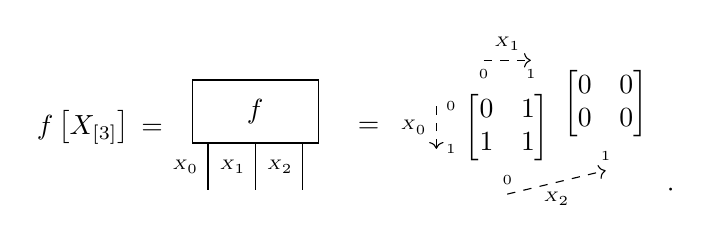
\begin{tikzpicture}[scale=1]

            \begin{scope}[shift={(-4,-0.2)}]
                \node[anchor=east] (A) at (-0.25,0.2) {$\formulaat{\catvariableof{[3]}}\,=$};
                \draw (0,0) rectangle (1.6,0.8);
                \node[anchor=center] (A) at (0.8,0.4) {$\formula$};
                \draw (0.2,0) -- (0.2,-0.6) node[midway,left] {\tiny $\catvariableof{0}$};
                \draw (0.8,0) -- (0.8,-0.6) node[midway,left] {\tiny $\catvariableof{1}$};
                \draw (1.4,0) -- (1.4,-0.6) node[midway,left] {\tiny $\catvariableof{2}$};
            \end{scope}

            \node[anchor=east] (A) at (-1.5,0) {$=$};
            \node (A) at (0,0) {
                $\begin{bmatrix}
                     0 & 1 \\
                     1 & 1
                \end{bmatrix}$
            };
            \node (A) at (1.25,0.3) {
                $\begin{bmatrix}
                     0 & 0 \\
                     0 & 0
                \end{bmatrix}$
            };
            \draw[<-,dashed] (-0.9,-0.275) node[right] {\tiny $1$} -- (-0.9,0.275) node [midway, left] {\tiny $\catvariableof{0}$} node[right] {\tiny $0$};
            \draw[->,dashed] (-0.3,0.85) node[below] {\tiny $0$} -- (0.3,0.85) node [midway, above] {\tiny $\catvariableof{1}$} node[below] {\tiny $1$};
            \draw[->,dashed] (0,-0.85) node[above] {\tiny $0$} -- (1.25,-0.55) node [midway, below] {\tiny $\catvariableof{2}$} node[above] {\tiny $1$};

            \node[anchor=east] (A) at (2.25,-0.8) {$\cdot$};
        \end{tikzpicture}
    \end{center}
    In the state set $\atomstates = \{0,1\}\times \{0,1\} \times \{0,1\}$ we have three models of the formula by the positions of the non-zero entries in the tensor, i.e. $\formulaat{\indexedcatvariableof{[3]}}=1$ if and only if
    \begin{align*}
        \catindexof{[3]}\in\{(1,0,0),(0,1,0),(1,1,0)\} \, .
    \end{align*}
    The formula $\formula$ is therefore satisfiable.
\end{example}

\paragraph{Model counts by contraction}
Each coordiante of the propositional formula is either a $1$ or $0$ encoding if the indexed state is a model of the formula or not.
In this way, the contraction $\contraction{\formula}$ counts the number of models of the propositional formula $\formula$.
One can therefore decide the satisfiability of a formula by checking if $\contraction{\formula}>0$.

\paragraph{CP decomposition}
Since the tensor $\formulaat{\shortcatvariables}$ is equal to one at index $x_{[d]}$ if and only if $x_{[d]}$ is a model of $\formula$, a propositional formula can be written as the sum over the one-hot encodings of its models.
\begin{center}
    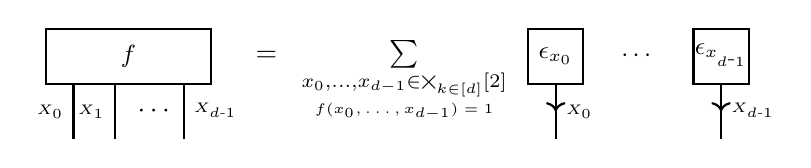
\begin{tikzpicture}[scale=0.35, thick]

    \draw (-1,-1) rectangle (5,-3);
    \node[anchor=center] (text) at (2,-2) {\corelabelsize ${\exformula}$};
    \draw[] (0,-3)--(0,-5) node[midway,left] {\colorlabelsize $\catvariableof{0}$};
    \draw[] (1.5,-3)--(1.5,-5) node[midway,left] {\colorlabelsize $\catvariableof{1}$};
    \node[anchor=center] (text) at (3,-4) {$\cdots$};
    \draw[] (4,-3)--(4,-5) node[midway,right] {\colorlabelsize $\catvariableof{\atomorder\shortminus1}$};


    \node[anchor=center] (text) at (7,-2) {${=}$};

    \node[anchor=center] (text) at (12,-2.5) {${\sum\limits_{\atomindices\in\atomstates}}$};
    \node[anchor=center] (text) at (12,-4) {\colorlabelsize $\exformula(\atomindices)=1$};

    \begin{scope}
        [shift={(19.5,1)}]

        \draw (-3,-2) rectangle (-1,-4);
        \node[anchor=center] (text) at (-2,-3) {\corelabelsize $\onehotmapof{\atomlegindexof{0}}$};
        \draw[->-] (-2,-4)--(-2,-6) node[midway,right] {\colorlabelsize $\catvariableof{0}$};

        \node[anchor=center] (text) at (1,-3) {\corelabelsize $\cdots$};

        \draw (3,-2) rectangle (5,-4);
        \node[anchor=center] (text) at (4,-3) {\corelabelsize $\onehotmapof{\atomlegindexof{\atomorder\shortminus1}}$};
        \draw[->-] (4,-4)--(4,-6) node[midway,right] {\colorlabelsize $\catvariableof{\atomorder\shortminus1}$};

    \end{scope}

\end{tikzpicture}
\end{center}
As already depicted one can exploit this summation to find a $\cpformat$ decomposition of the formula.
To this we enumerate the models $\shortcatindices^{\decindex}$ of $\formula$ by a decomposition variable $\decvariable$ with values $\decindex\in[\contraction{\formula}]$ and define for $\catenumeratorin$ cores with slices
\begin{align*}
    \hypercoreofat{\catenumerator}{\catvariableof{\catenumerator},\indexeddecvariable}
    = \onehotmapofat{\catindexof{\catenumerator}^{\decindex}}{\catvariableof{\catenumerator}} \, .
\end{align*}

\begin{example}\label{exa:propFormulaBasCP}
    For the formula described in \exaref{exa:propFormulaCoordinatewise}, we have
    \begin{align*}
        \formulaat{\catvariableof{[3]}}
        &= \left(\tbasisat{\catvariableof{0}} \otimes \fbasisat{\catvariableof{1}} \otimes \fbasisat{\catvariableof{2}}\right)
        + (\fbasisat{\catvariableof{0}} \otimes \tbasisat{\catvariableof{1}} \otimes \fbasisat{\catvariableof{2}}) \\
        &\quad+ (\tbasisat{\catvariableof{0}} \otimes \tbasisat{\catvariableof{1}} \otimes \fbasisat{\catvariableof{2}}) \, .
    \end{align*}
    Note that we have $\contraction{\formulawith}=3$ and we can interpret this sum as a $\cpformat$ decomposition of $\formula$ with rank $3$.
%    where we denote the vectors $\tbasisat{Y} = [0,1]^T$ and $\fbasisat{Y} = [1,0]^T$.
    We use the decomposition to evaluate the formula $\formula$ at $\catindexof{[3]} = (1,1,0)$ and get
    \begin{align*}
        \formulaat{\indexedcatvariableof{[3]}}
        &= \left(\tbasisat{\catvariableof{0}=1} \otimes \fbasisat{\catvariableof{1}=1} \otimes \fbasisat{\catvariableof{2}=0}\right) \\
       &\quad + (\fbasisat{\catvariableof{0}=1} \otimes \tbasisat{\catvariableof{1}=1} \otimes \fbasisat{\catvariableof{2}=0}) \\
       &\quad + (\tbasisat{\catvariableof{0}=1} \otimes \tbasisat{\catvariableof{1}=1} \otimes \fbasisat{\catvariableof{2}=0}) \\
        &=  1\cdot 0 \cdot 1 + 0\cdot 1 \cdot 1 + 1 \cdot 1 \cdot 1 = 1 \, ,
    \end{align*}
    which verifies that $\catindexof{[3]} = (1,1,0)$ is a model of the formula $\formula$.
\end{example}

\paragraph{Basis encoding}
Representing booleans by elements in $\{0,1\}$ leads to the problem, that negation is an affine transformation and can not be represented by multilinear tensors. %~\cite[Section 4.1.1]{goessmann_tensor-network_2025}.
Therefore, instead of using this \emph{coordinate calculus} an approach based on \emph{basis calculus} is employed, which is explained in this section.
To be able to express different kinds of connectives and finally any propositional formula by multi-linear tensors, booleans are encoded by one-hot encodings as defined in \defref{def:onehotenc}.
Propositional formulas $\formula$ can be expressed in terms of a tensor describing the mapping and its negation by
\begin{align}
    \label{eq:basisencboolean}
    \bencodingofat{\formula}{\indexedheadvariableof{\formula},\indexedshortcatvariables}
    = \begin{cases}
          1 & \ifspace \formulaat{\indexedshortcatvariables} = \headindexof{\formula}\\
          0 & \text{else}
    \end{cases}.
\end{align}
This basis encoding $\bencodingofat{\formula}{\headvariableof{\formula},\shortcatvariables} \in \{0,1\}^{2\times 2^d}$ then has the form
\begin{align}
    \label{eq:basisencnegsum}
    \bencodingofat{\formula}{\headvariableof{\formula},\shortcatvariables}
    = \tbasisat{\headvariableof{\formula}} \otimes \formulaat{\shortcatvariables}
    + \fbasisat{\headvariableof{\formula}} \otimes \lnot\formulaat{\shortcatvariables} \, .
\end{align}
In our graphical notation this property is visualized by
\begin{center}
    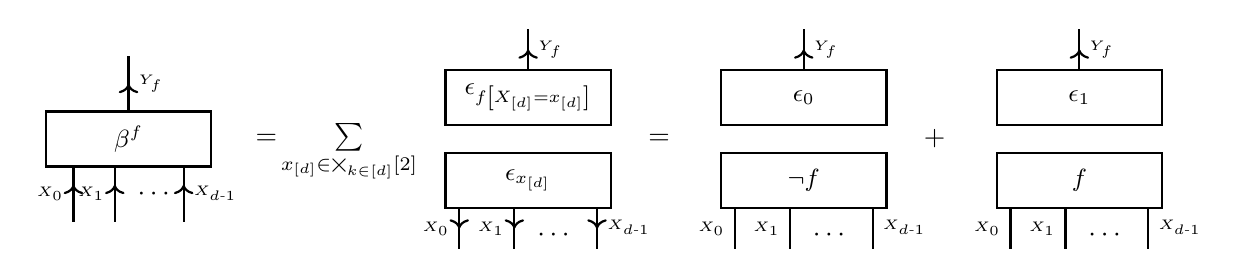
\begin{tikzpicture}[scale=0.35, thick] % , baseline = -3.5pt

    \draw[->-] (2,-1)--(2,1) node[midway,right] {\colorlabelsize $\formulavar$};
    \draw (-1,-1) rectangle (5,-3);
    \node[anchor=center] (text) at (2,-2) {\corelabelsize $\bencodingof{\exformula}$};
    \draw[-<-] (0,-3)--(0,-5) node[midway,left] {\colorlabelsize $\catvariableof{0}$};
    \draw[-<-] (1.5,-3)--(1.5,-5) node[midway,left] {\colorlabelsize $\catvariableof{1}$};
    \node[anchor=center] (text) at (3,-4) {$\cdots$};
    \draw[-<-] (4,-3)--(4,-5) node[midway,right] {\colorlabelsize $\catvariableof{\atomorder\shortminus1}$};


    \node[anchor=center] (text) at (7,-2) {${=}$};

    \node[anchor=center] (text) at (10,-2.5) {${\sum\limits_{\shortcatindices\in\atomstates}}$};

    \begin{scope}
    [shift={(15.5,-0.5)}]

        \draw (-2,1) rectangle (4,-1);
        \node[anchor=center] (text) at (1,0) {\corelabelsize $\onehotmapof{\exformulaat{\indexedshortcatvariables}}$};
        \draw[->-] (1,1)--(1,2.5) node[midway,right] {\colorlabelsize $\formulavar$};

        \draw (-2,-2) rectangle (4,-4);
        \node[anchor=center] (text) at (1,-3) {\corelabelsize $\onehotmapof{\shortcatindices}$};

        \draw[->-] (-1.5,-4)--(-1.5,-5.5) node[midway,left] {\colorlabelsize $\catvariableof{0}$};
        \draw[->-] (0.5,-4)--(0.5,-5.5) node[midway,left] {\colorlabelsize $\catvariableof{1}$};
        \node[anchor=center] (text) at (2,-5) {$\cdots$};
        \draw[->-] (3.5,-4)--(3.5,-5.5) node[midway,right] {\colorlabelsize $\catvariableof{\atomorder\shortminus1}$};

    \end{scope}

    \node[anchor=center] (text) at (21.25,-2) {${=}$};

    \begin{scope} [shift={(25.5,-0.5)}]

        \draw (-2,1) rectangle (4,-1);
        \node[anchor=center] (text) at (1,0) {\corelabelsize $\onehotmapof{0}$};
        \draw[->-] (1,1)--(1,2.5) node[midway,right] {\colorlabelsize $\formulavar$};

        \draw (-2,-2) rectangle (4,-4);
        \node[anchor=center] (text) at (1,-3) {\corelabelsize $\lnot\formula$};%$\sum_{\shortcatindices \wcols \formula(\shortcatindices)=0}\onehotmapof{\shortcatindices}$};

        \draw[] (-1.5,-4)--(-1.5,-5.5) node[midway,left] {\colorlabelsize $\catvariableof{0}$};
        \draw[] (0.5,-4)--(0.5,-5.5) node[midway,left] {\colorlabelsize $\catvariableof{1}$};
        \node[anchor=center] (text) at (2,-5) {$\cdots$};
        \draw[] (3.5,-4)--(3.5,-5.5) node[midway,right] {\colorlabelsize $\catvariableof{\atomorder\shortminus1}$};

    \end{scope}


    \node[anchor=center] (text) at (31.25,-2) {${+}$};

    \begin{scope} [shift={(35.5,-0.5)}]

        \draw (-2,1) rectangle (4,-1);
        \node[anchor=center] (text) at (1,0) {\corelabelsize $\onehotmapof{1}$};
        \draw[->-] (1,1)--(1,2.5) node[midway,right] {\colorlabelsize $\formulavar$};

        \draw (-2,-2) rectangle (4,-4);
        \node[anchor=center] (text) at (1,-3) {\corelabelsize $\formula$};%$\sum_{\shortcatindices \wcols \formula(\shortcatindices)=1}\onehotmapof{\shortcatindices}$};

        \draw[] (-1.5,-4)--(-1.5,-5.5) node[midway,left] {\colorlabelsize $\catvariableof{0}$};
        \draw[] (0.5,-4)--(0.5,-5.5) node[midway,left] {\colorlabelsize $\catvariableof{1}$};
        \node[anchor=center] (text) at (2,-5) {$\cdots$};
        \draw[] (3.5,-4)--(3.5,-5.5) node[midway,right] {\colorlabelsize $\catvariableof{\atomorder\shortminus1}$};

    \end{scope}

\end{tikzpicture}
\end{center}
We further provide a more detailed example in coordinate sensitive notation in the following.
\begin{example}[Logical Negation and Conjunction]
    \label{exa:bencodingNegCon} %\cite[Example 4.9]{goessmann_tensor-network_2025}
    The basis encodings of the negation $\notucon: [2]\rightarrow [2]$ is the matrix
    \begin{center}
        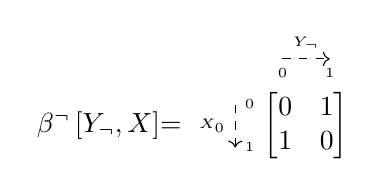
\begin{tikzpicture}[scale=1]
            \node (A) at (-2.5,0) {$\bencodingofat{\lnot}{\headvariableof{\lnot},\catvariable}$=};
            \node (A) at (0,0) {
                $\begin{bmatrix}
                     0 & 1 \\
                     1 & 0
                \end{bmatrix}$
            };
            \draw[<-,dashed] (-0.9,-0.275) node[right] {\tiny $1$} -- (-0.9,0.275) node [midway, left] {\tiny $\catvariableof{0}$} node[right] {\tiny $0$};
            \draw[->,dashed] (-0.3,0.85) node[below] {\tiny $0$} -- (0.3,0.85) node [midway, above] {\tiny $\headvariableof{\lnot}$} node[below] {\tiny $1$};
        \end{tikzpicture}
    \end{center}
    The $2$-ary conjunctions $\land:  [2]\times[2] \rightarrow[2]$ is encoded by the order-$3$ tensor
    \begin{center}
        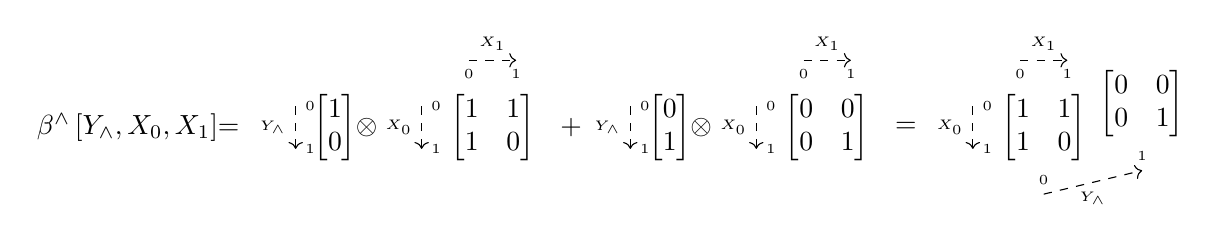
\begin{tikzpicture}[scale=1]
            \node (A) at (-4.5,0) {$\bencodingofat{\land}{\headvariableof{\land},\catvariableof{0},\catvariableof{1}}$=};

            \begin{scope}[shift={(0,0)}]
                \node(B) at (-2,0){
                    $\begin{bmatrix}
                         1 \\
                         0
                    \end{bmatrix}$
                };
                \draw[<-,dashed] (-2.5,-0.275) node[right] {\tiny $1$} -- (-2.5,0.275) node [midway, left] {\tiny $\headvariableof{\land}$} node[right] {\tiny $0$};
                \node (A) at (-1.6,0) {$\otimes$};
                \node (A) at (0,0) {
                    $\begin{bmatrix}
                         1 & 1 \\
                         1 & 0
                    \end{bmatrix}$
                };
                \draw[<-,dashed] (-0.9,-0.275) node[right] {\tiny $1$} -- (-0.9,0.275) node [midway, left] {\tiny $\catvariableof{0}$} node[right] {\tiny $0$};
                \draw[->,dashed] (-0.3,0.85) node[below] {\tiny $0$} -- (0.3,0.85) node [midway, above] {\tiny $\catvariableof{1}$} node[below] {\tiny $1$};
            \end{scope}

            \begin{scope}[shift={(4.25,0)}]

                \node[anchor=center] (A) at (-3.25,0) {$+$};

                \node(B) at (-2,0){
                    $\begin{bmatrix}
                         0 \\
                         1
                    \end{bmatrix}$
                };
                \draw[<-,dashed] (-2.5,-0.275) node[right] {\tiny $1$} -- (-2.5,0.275) node [midway, left] {\tiny $\headvariableof{\land}$} node[right] {\tiny $0$};
                \node (A) at (-1.6,0) {$\otimes$};
                \node (A) at (0,0) {
                    $\begin{bmatrix}
                         0 & 0 \\
                         0 & 1
                    \end{bmatrix}$
                };
                \draw[<-,dashed] (-0.9,-0.275) node[right] {\tiny $1$} -- (-0.9,0.275) node [midway, left] {\tiny $\catvariableof{0}$} node[right] {\tiny $0$};
                \draw[->,dashed] (-0.3,0.85) node[below] {\tiny $0$} -- (0.3,0.85) node [midway, above] {\tiny $\catvariableof{1}$} node[below] {\tiny $1$};
            \end{scope}

            \begin{scope}[shift={(7,0)}]
                \node[anchor=center] (A) at (-1.75,0) {$=$};

                \node (A) at (0,0) {
                    $\begin{bmatrix}
                         1 & 1 \\
                         1 & 0
                    \end{bmatrix}$
                };
                \node (A) at (1.25,0.3) {
                    $\begin{bmatrix}
                         0 & 0 \\
                         0 & 1
                    \end{bmatrix}$
                };
                \draw[<-,dashed] (-0.9,-0.275) node[right] {\tiny $1$} -- (-0.9,0.275) node [midway, left] {\tiny $\catvariableof{0}$} node[right] {\tiny $0$};
                \draw[->,dashed] (-0.3,0.85) node[below] {\tiny $0$} -- (0.3,0.85) node [midway, above] {\tiny $\catvariableof{1}$} node[below] {\tiny $1$};
                \draw[->,dashed] (0,-0.85) node[above] {\tiny $0$} -- (1.25,-0.55) node [midway, below] {\tiny $\headvariableof{\land}$} node[above] {\tiny $1$};
            \end{scope}
        \end{tikzpicture}
    \end{center}
    Further, the $2$-ary disjunction $\lor:  [2]\times[2] \rightarrow[2]$ is encoded by the order-$3$ tensor
    \begin{center}
        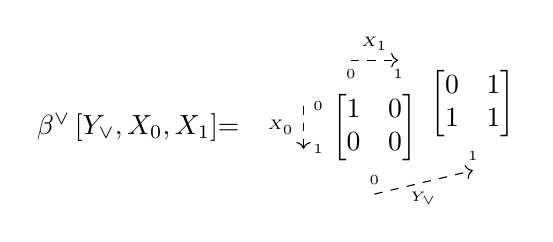
\begin{tikzpicture}[scale=1]
            \node (A) at (-3,0) {$\bencodingofat{\lor}{\headvariableof{\lor},\catvariableof{0},\catvariableof{1}}$=};
            \node (A) at (0,0) {
                $\begin{bmatrix}
                     1 & 0 \\
                     0 & 0
                \end{bmatrix}$
            };
            \node (A) at (1.25,0.3) {
                $\begin{bmatrix}
                     0 & 1 \\
                     1 & 1
                \end{bmatrix}$
            };
            \draw[<-,dashed] (-0.9,-0.275) node[right] {\tiny $1$} -- (-0.9,0.275) node [midway, left] {\tiny $\catvariableof{0}$} node[right] {\tiny $0$};
            \draw[->,dashed] (-0.3,0.85) node[below] {\tiny $0$} -- (0.3,0.85) node [midway, above] {\tiny $\catvariableof{1}$} node[below] {\tiny $1$};
            \draw[->,dashed] (0,-0.85) node[above] {\tiny $0$} -- (1.25,-0.55) node [midway, below] {\tiny $\headvariableof{\lor}$} node[above] {\tiny $1$};
        \end{tikzpicture}
    \end{center}
\end{example}

\paragraph{Interpretation as \CompActNets{}}
The propositional formula and its negation can be represented by that tensor by
\begin{align*}
    \formulaat{\shortcatvariables}
    = \contractionof{\tbasisat{\headvariableof{\formula}},\bencodingofat{\formula}{\headvariableof{\formula},\shortcatvariables}}{\shortcatvariables}
    \andspace
    \lnot\formulaat{\shortcatvariables}
    = \contractionof{\fbasisat{\headvariableof{\formula}},\bencodingofat{\formula}{\headvariableof{\formula},\shortcatvariables}}{\shortcatvariables} \, .
\end{align*}
Both $\formula$ and $\lnot\formula$ are thus \ComputationActivationNetworks{} to the statistic $\{\formula\}$ and the hard activation tensor $\tbasisat{\headvariableof{\formula}}$, respectively $\fbasisat{\headvariableof{\formula}}$.
%This representation of propositional formulas with respect to basis encoding thus leads to \ComputationActivationNetworks{}, which were also used to describe probability distributions in the last section.
%In this way the soft and hard logic can be combined in one framework.

\subsection{Syntactical Decomposition of Propositional Formulas}

Propositional formulas of concern often have a syntactical specification as composed functions.
We can therefore apply the neural paradigm to find efficient representations of them.

\begin{definition}[Syntactical Decompositions]
    \label{def:syntacticalDecomposition}
    A syntactical decomposition of a propositional formula $\exformula$ is a decomposition hypergraph (see \defref{def:decompositionHypergraph}) such that all nodes are decorated with the dimension $\catdimof{\node}=2$ and composition function $\exformula$.
\end{definition}

Thus we have a tensor network representation of any propositional formula based on its syntactical decomposition, where the hypergraph of the syntactical decomposition equals the hypergraph of the representing tensor network.

\input{../examples/logical_paradigm/prop_formula_syntax}

%\begin{lemma}
%    \label{lem:formulaDecomp}
%    Let $\formulaat{\shortcatvariables}$ be a composition of a $\seldim$-ary connective formula $\exconnective$ and propositional formulas $\formulaofat{\selindex}{\shortcatvariables}$, where $\selindexin$, i.e. for $\shortcatindices\in\atomstates$ we have
%    \begin{align*}
%        \formulaat{\indexedshortcatvariables}
%        = \exconnective\left(\formulaofat{0}{\indexedshortcatvariables}, \dots, \formulaofat{\seldim-1}{\indexedshortcatvariables}\right) \, .
%    \end{align*}
%    Then we have
%    \begin{align*}
%        \bencodingofat{\formula}{\headvariableof{\formula},\shortcatvariables}
%        = \contractionof{
%            \{\bencodingofat{\exconnective}{\headvariableof{\formula},\headvariableof{[\seldim]}}\}
%            \cup \{\bencodingofat{\formulaof{\selindex}}{\headvariableof{\selindex},\shortcatvariables} \wcols \selindexin\}
%        }{\headvariableof{\formula},\shortcatvariables} \, .
%    \end{align*}
%\end{lemma}
%\begin{proof}
%    This can be shown on each index $\shortcatindices$.
%\end{proof}

%\begin{definition}
%    \label{def:formulaDecomposition}
%    A syntactical hypergraph is a directed acyclic hypergraph $\graph=(\nodes,\edges)$ such that
%    \begin{itemize}
%        \item each hyperedge $\edge=(\incomingnodes,\outgoingnodes)$ has exactly one outgoing node, i.e. $\cardof{\outgoingnodes}=1$
%        \item each node $\nodein$ carries a boolean variable $\headvariableof{\node}$ and appears at most once as the outgoing node of a hyperedge % well-definedness
%        \item each hyperedge $(\incomingnodes,\{\node\})$ with $\incomingnodes\neq\varnothing$ is decorated by a propositional formula
%        \begin{align*}
%            \connectiveofat{\node}{\headvariableof{\incomingnodes}} \defcols \bigtimes_{\node\in\incomingnodes} [2] \rightarrow [2]
%        \end{align*}
%        \item the nodes not appearing as an outgoing node are labeled by $[\atomorder]$
%    \end{itemize}
%    We say that the syntactical hypergraph is single-rooted, if exactly one node $\secnode$ does not appear as an incoming node of a hyperedge.
%    In this case this unique node is called the root node. % head node
%    We assign atomic formulas to the nodes $[\atomorder]$ and recursively assign to each further node $\node$ a node formula % connective $\connectiveofat{\node}{\headvariableof{\incomingnodes}}$.
%    \begin{align*}
%        \formulaofat{\node}{\indexedshortcatvariables}
%        = \connectiveofat{\node}{[\formulaofat{\thirdnode}{\indexedshortcatvariables}\wcols\thirdnode\in\incomingnodes]} \quad \forall\shortcatindicesin\, ,
%    \end{align*}
%    where $\incomingnodes$ are the incoming nodes in the unique hyperedge with outgoing nodes $\{\node\}$.
%    We call the formula $\exformulaat{\shortcatvariables}\coloneqq\formulaofat{\secnode}{\shortcatvariables}$ to the root note $\secnode$ the syntactical composition of $\graph$ and $\graph$ is a syntactical decomposition of $\exformula$.
%\end{definition}
%
%%We now show, that the propositional formula allows for a decomposition into connective formulas, its basis encoding decomposes into the basis encodings of the connective formulas.
%
%\begin{theorem}
%    \label{the:formulaDecompositionRep}
%    For any syntactical hypergraph $\graph$ with composition $\exformula$ we have
%    \begin{align*}
%        \exformulaat{\shortcatvariables}
%        = \breakablecontractionof{
%            &\left\{
%                 \bencodingofat{\connectiveof{\node}}{\headvariableof{\node},\headvariableof{\incomingnodes}} \wcols (\incomingnodes,\{\node\})\in\edges
%            \right\} \cup \\
%            & \{\identityat{\headvariableof{\atomenumerator},\catvariableof{\atomenumerator}} \wcols \atomenumeratorin\}
%            \cup \{\tbasisat{\headvariableof{\secnode}}\}
%        }{\shortcatvariables} \, .
%    \end{align*}
%\end{theorem}
%\begin{proof}
%    One can show this theorem by induction over the node formulas of the syntactical hypergraph, from the leafs to the root and iteratively applying \lemref{lem:formulaDecomp}.
%\end{proof}
%
%Thus we have a tensor network representation of any propositional formula based on its syntactical decomposition, where the hypergraph of the syntactical decomposition equals the hypergraph of the representing tensor network.
%

\subsection{Entailment Decision by Contractions}

We have already seen that the contraction of a propositional formula counts its models.
This allows to define entailment between two propositional formulas as follows.
To generalize the treatment, we do not demand any more that the variables of a formula are of dimension $2$.
We further use $\lnot\formulawith=\oneswith-\formulawith$.

\begin{definition}[Entailment of propositional formulas]
    \label{def:logicalEntailment}
    Given two propositional formulas $\kb$ and $\formula$ we say that $\kb$ entails $\formula$, denoted by $\kb\models\formula$, if any model of $\kb$ is also a model of $\formula$, that is
    \begin{align*}
        \contraction{\kbwith,\lnot\formulawith}=0 \, .
    \end{align*}
    If $\kb\models\lnot\formula$ holds (i.e. $\contraction{\kbwith,\formulawith}$=0), we say that $\kb$ contradicts $\formula$.
\end{definition}

% Relation to classical definition of entailment
Classically (see e.g. \cite{russell_artificial_2021}) entailment in propositional logics is defined as the unsatisfiability of $\kb\land\lnot\exformula$.
This is equivalent to \defref{def:logicalEntailment}, since $\contraction{\kbwith,\lnot\formulawith}=0$ is equivalent to $\contraction{(\kb \land (\lnot\exformula))[\shortcatvariables]}=0$, which is the unsatisfiability of $\kb\land\lnot\exformula$.

%Entailment is the central operation of "logical inference", i.e. deduce true statements from known statements.
%In the tensor network representation, these entailments can be decided by contracting the whole representing tensor with the statement, that needs to be checked.

\begin{example}[$\sudokunum^2\,\times \,\sudokunum^2$ Sudoku]
    \label{exa:sudokuEntailment}%{\alex{Attempt to match the above Sudoku example with our notation of boolean variables and the entailment formalism}}
    We index the rows and the columns by tuples $(r0,r1)$ and $(co,c1)$, where $r0,r1,c0,c1\in[\sudokunum]$. The first index indicates the block and the second counts the row or column inside that block.
    For each $r0,r1,c0,c1\in[\sudokunum]$ and $i\in[\sudokunum^2]$ we then define an atomic variable $\catvariableof{r0,r1,c0,c1,i}\in\{0,1\}$ indicating whether in the row $(r0,r1)$ and column $(co,c1)$ the number $i$ is written.
    The Sudoku rules then amount to the formula
    \begin{align*}
        \sudokukbof{\sudokunum}  \coloneqq
        &\left( \bigwedge_{r0,r1,c0,c1\in[\sudokunum]} \left( \woneoplus_{i\in[\sudokunum^2]} \catvariableof{r0,r1,c0,c1,i} \right) \right) \land
        \left( \bigwedge_{r0,r1\in[\sudokunum], i\in[\sudokunum^2]} \left( \woneoplus_{c0,c1\in[\sudokunum]} \catvariableof{r0,r1,c0,c1,i} \right) \right) \land \\
        &\left( \bigwedge_{c0,c1\in[\sudokunum], i\in[\sudokunum^2]} \left( \woneoplus_{c0,c1\in[\sudokunum]} \catvariableof{r0,r1,c0,c1,i} \right) \right) \land
        \left( \bigwedge_{r0,c0\in[\sudokunum], i\in[\sudokunum^2]} \left( \woneoplus_{r1,c1\in[\sudokunum]} \catvariableof{r0,r1,c0,c1,i} \right) \right) \, ,
    \end{align*}
    where $\woneoplus$ is the $\sudokunum^2$-ary exclusive or connective (that is $1$ if and only if exactly one of the arguments is $1$).
    The four outer brackets in $\kb$ mark the constraints that at each position exactly one number is assigned, further that in each row each number is assigned once, and similar for the columns and the squares of the board.
    When solving a specific Sudoku instance, one typically knows from an initial board assignment $\sudokustartevidence$ a collection of atomic variables, which hold, and needs to find further atomic variables, which are entailed.
    This means, we need to decide for each $(r_0,r_1,c_0,c_1,i)\notin \sudokustartevidence$ whether the Sudoku rules and the initial board imply that the atomic variable $\catvariableof{r0,r1,c0,c1,i}$ (i.e. assignment to the board) is true
    \begin{align*}
        \sudokukbof{\sudokunum} \land \left(\bigwedge_{(r_0,r_1,c_0,c_1,i)\in \sudokustartevidence} \catvariableof{r0,r1,c0,c1,i} \right) \models \catvariableof{r0,r1,c0,c1,i}
    \end{align*}
    or false
    \begin{align*}
%        \label{eq:sudokukb}
        \kb \land \left(\bigwedge_{(r_0,r_1,c_0,c_1,i)\in \sudokustartevidence} \catvariableof{r0,r1,c0,c1,i} \right) \models \lnot\catvariableof{r0,r1,c0,c1,i} \, .
    \end{align*}
%    In other words, for each assignment to the board, that fulfills the Sudoku rules and the initial board, do we write the number $n$ in row $(r0,r1)$ and column $(c0,c1)$?
    If and only if the Sudoku has a unique solution given the initial board assignment $\sudokustartevidence$, exactly one of these entailment statements holds for each $(r_0,r_1,c_0,c_1,i)\notin \sudokustartevidence$.
    Deciding which is equivalent to solving the Sudoku.
%    We model Sudoku as a hypergraph of
%    \begin{itemize}
%        \item Nodes labeled by $\sudokunum^6$ tuples $(r0,r1,c0,c1,i)$:
%        \begin{align*}
%            \nodes = \{(r0,r1,c0,c1,i) \wcols r0,r1,c0,c1 \in [\sudokunum]\ncond i \in [\sudokunum^2]\}
%        \end{align*}
%        \item Hyperedges by the $4\cdot \sudokunum^4$ constraints (implementing the position, row, columns and square contraints):
%        \begin{align*}
%            \edges =& \big\{\{(r0,r1,c0,c1,i) \wcols r0,r1,c0,c1\in[\sudokunum]\} \wcols r0,r1,c0,c1\in[\sudokunum]\big\} \cup \\
%            &\big\{\{(r0,r1,c0,c1,i) \wcols r0,r1,c0,c1\in[\sudokunum]\} \wcols r0,r1\in[\sudokunum], i\in[\sudokunum^2]\big\} \cup \\
%            &\big\{\{(r0,r1,c0,c1,i) \wcols r0,r1,c0,c1\in[\sudokunum]\} \wcols c0,c1\in[\sudokunum], i\in[\sudokunum^2]\big\} \cup \\
%            &\big\{\{(r0,r1,c0,c1,i) \wcols r0,r1,c0,c1\in[\sudokunum]\} \wcols r0,c0\in[\sudokunum], i\in[\sudokunum^2]\big\} \cup
%        \end{align*}
%        Each hypercore is carried by a tensor representing the logical formula $\woneoplus$ on $\sudokunum^2$ boolean variables.
%    \end{itemize}

    For a more concrete example, let $n=2$ and
    \begin{align*}
        \sudokustartevidence = \{&(0,0,0,0,0),(0,0,1,0,2),(0,0,1,1,1), %first row
        (0,1,0,1,1), \\ %second row
        &(1,0,1,0,3), %third row
        (1,1,0,0,3),(1,1,0,1,2) %fourth row
        \} \, .
    \end{align*}
    We visualize this evidence by writing $i+1$ in a grid cell $(r0,r1,c0,c1)$ to indicate that $(r0,r1,c0,c1,i)\in \sudokustartevidence$:
    \begin{center}
        \begin{sudoku4x4}
            \matrix[sudokumatrix] (M) at (0,0) {
                1 & \ & 3 & 2 \\
                \ & 2 & \  & \  \\
                \ & \ & 4 & \ \\
                4 & 3 &  \ & \  \\
            };
            \draw[thick]([yshift=9.5pt,xshift=-0.6pt]M-1-2.east) -- ([yshift=-9.5pt,xshift=-0.6pt]M-4-2.east);
            \draw[thick]([xshift=-9.5pt,yshift=0.6pt]M-2-1.south) -- ([xshift=9.5pt,yshift=0.6pt]M-2-4.south);
        \end{sudoku4x4}
    \end{center}
    After deriving a sparse tensor network representations in \exaref{exa:sudokuDecomposition}, we demonstrate a solution algorithm to solve this instance in \exaref{exa:sudokuEntailment}.
\end{example}

\subsection{Efficient Representation of Knowledge Bases}

We now investigate the representation of propositional knowledge bases $\kb=\{\formulaof{\selindex}\wcols\selindexin\}$, which are sets of propositional formulas $\formulaof{\selindex}$.
The conjunction of these formulas is the knowledge base formula
\begin{align*}
    \kbwith
    = \bigwedge_{\selindexin} \formulaofat{\selindex}{\shortcatvariables} \, .
\end{align*}
To show efficient repesentations we will use the following identities.

\begin{lemma}[Computation Network Symmetries]
    \label{lem:comNetSymmetries}
    We have for the $\catorder$-ary $\land$-connective (where $\catorder\in\nn$) and the unary $\lnot$-connective that
    \begin{align*}
        \contractionof{\tbasisat{\headvariable},\bencodingofat{\land}{\headvariable,\shortcatvariables}}{\shortcatvariables}
        = \bigotimes_{\catenumeratorin} \tbasisat{\catvariableof{\catenumerator}}
        \andspace
        \contractionof{\tbasisat{\headvariable},\bencodingofat{\lnot}{\headvariable,\catvariable}}{\catvariable}
        = \fbasisat{\catvariable} \, .
    \end{align*}
\end{lemma}
\begin{proof}
    Follows directly from the definitions of the basis encodings and the connectives.
\end{proof}

\begin{example}[Computation Network Symmetries]
    %see the notebook: \url{https://colab.research.google.com/drive/1p2wp61fFMu0otnfFhKoNsLiCNfWpuEsn?usp=sharing}
    For the propositional formula $\formulaat{\catvariableof{[3]}}={(\catvariableof{0} \lor \catvariableof{1}) \land \lnot \catvariableof{2}}$ (see \exaref{exa:propFormulaCoordinatewise}), we can write the formula in terms of a \ComputationActivationNetwork{} with activation tensor $\tbasis$ and computation network decomposed by the basis encodings. First, it is written with one activation vector. Second, we see that it can also be interpreted with multiple features.
    \begin{center}
        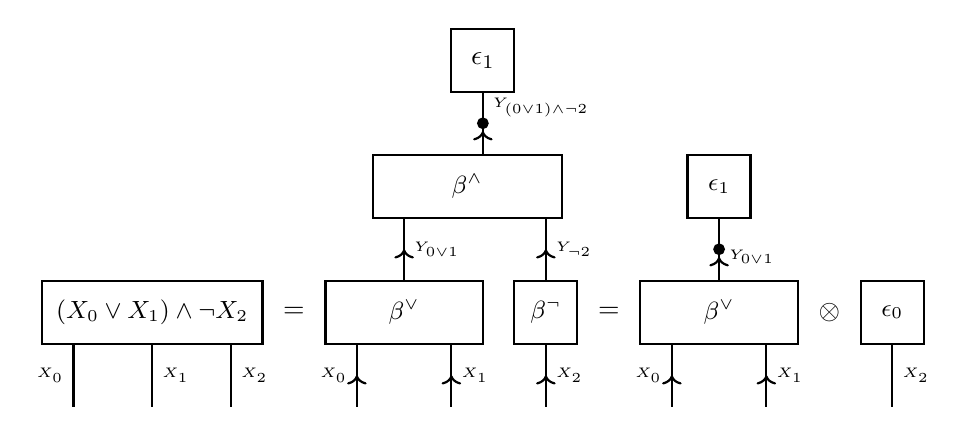
\begin{tikzpicture}[scale=0.4, yscale=-1, thick] % , baseline = -3.5pt

            \draw[] (-2,1)--(-2,-1) node[midway,left] {\colorlabelsize $\catvariableof{0}$};
            \draw[] (0.5,1)--(0.5,-1) node[midway,right] {\colorlabelsize $\catvariableof{1}$};
            \draw[] (3,1)--(3,-1) node[midway,right] {\colorlabelsize $\catvariableof{2}$};
            \draw (-3,-1) rectangle (4, -3);
            \node[anchor=center] (text) at (0.5,-2) {\corelabelsize $(\catvariableof{0} \lor \catvariableof{1}) \land \lnot \catvariableof{2}$};
            %\draw[->-] (1.5,-3)--(1.5,-5) node[midway,right] {\colorlabelsize $\headvariableof{a \land b \land \lnot c}$};

            \node[anchor=center] (text) at (5,-2) {${=}$};


            \begin{scope}
            [shift={(7,0)}]

                \draw[->-] (0,1)--(0,-1) node[midway,left] {\colorlabelsize $\catvariableof{0}$};
                \draw[->-] (3,1)--(3,-1) node[midway,right] {\colorlabelsize $\catvariableof{1}$};
                \draw[->-] (6,1)--(6,-1) node[midway,right] {\colorlabelsize $\catvariableof{2}$};

                \draw (-1,-1) rectangle (4, -3);
                \node[anchor=center] (text) at (1.5,-2) {\corelabelsize $\bencodingof{\lor}$};

                \draw[->-] (1.5,-3) --(1.5,-5) node[midway,right]{\colorlabelsize $\headvariableof{0 \lor 1}$};

                \draw (5,-1) rectangle (7, -3);
                \node[anchor=center] (text) at (6,-2) {\corelabelsize $\bencodingof{\lnot}$};

                \draw[->-] (6,-3) --(6,-5) node[midway,right]{\colorlabelsize $\headvariableof{\lnot 2}$};

                \draw (0.5,-5) rectangle (6.5,-7);
                \node[anchor=center] (text) at (3.5,-6) {\corelabelsize $\bencodingof{\land}$};

                \draw[->-] (4,-7) -- (4,-8.5) node[right] {\colorlabelsize $\headvariableof{(0 \lor 1) \land \lnot 2}$};
                \drawvariabledot{4}{-8}
                \draw[] (4,-8) -- (4,-9);
                \draw (3,-9) rectangle (5,-11);
                \node[anchor=center] (text) at (4,-10) {$\tbasis$};

            \end{scope}

            \node[anchor=center] (text) at (15,-2) {${=}$};

            \begin{scope}
            [shift={(17,0)}]

                \draw[->-] (0,1)--(0,-1) node[midway,left] {\colorlabelsize $\catvariableof{0}$};
                \draw[->-] (3,1)--(3,-1) node[midway,right] {\colorlabelsize $\catvariableof{1}$};
                \draw[] (7,1)--(7,-1) node[midway,right] {\colorlabelsize $\catvariableof{2}$};

                \draw (-1,-1) rectangle (4, -3);
                \node[anchor=center] (text) at (1.5,-2) {\corelabelsize $\bencodingof{\lor}$};

                \draw (1.5,-4.5) -- (1.5,-5);
                \draw[->-] (1.5,-3) --(1.5,-4.5) node[midway,right]{\colorlabelsize $\headvariableof{0 \lor 1}$};

                \drawvariabledot{1.5}{-4}
                \draw (0.5,-5) rectangle (2.5,-7);
                \node[anchor=center] (text) at (1.5,-6) {\corelabelsize $\tbasis$};

                \node[anchor=center] (text) at (5,-2) {$\otimes$};


                \draw (6,-1) rectangle (8, -3);
                \node[anchor=center] (text) at (7,-2) {\corelabelsize $\fbasis$};

                %\draw[->-] (6,-3) --(6,-5) node[midway,right]{\colorlabelsize $\headvariableof{\lnot c}$};


                %\draw (0.5,-5) rectangle (6.5,-7);
                %\node[anchor=center] (text) at (3.5,-6) {\corelabelsize $\bencodingof{\land}$};

                %\draw[->-] (4,-7) -- (4,-8.5) node[right] {\colorlabelsize $\headvariableof{(a \lor b) \land \lnot c}$};
                %\drawvariabledot{4}{-8}
                %\draw[] (4,-8) -- (4,-9);
                %\draw (3,-9) rectangle (5,-11);
                %\node[anchor=center] (text) at (4,-10) {$\tbasis$};

            \end{scope}

        \end{tikzpicture}
    \end{center}
\end{example}


We use this to decompose knowledge bases into their individual formulas as follows.

\begin{theorem}
    \label{the:kbDecomposition}
    For any knowledge base $\kbwith = \bigwedge_{\selindexin} \formulaofat{\selindex}{\shortcatvariables}$ it holds that
    \begin{align*}
        \kbwith
        = \contractionof{\{\formulaofat{\selindex}{\shortcatvariables} \wcols \selindexin\}}{\shortcatvariables} \, .
    \end{align*}
\end{theorem}
\begin{proof}
    With \lemref{lem:comNetSymmetries} we have
    \begin{align*}
        \kbwith
        &= \contractionof{\{\tbasisat{\headvariableof{\land}},\bencodingofat{\land}{\headvariableof{\land},\headvariables}\}
            \cup \{\bencodingofat{\formulaof{\selindex}}{\headvariableof{\selindex},\shortcatvariables}\wcols \selindexin\}}{\shortcatvariables} \\
        &= \contractionof{
            \bigcup_{\selindexin} \{\tbasisat{\headvariableof{\selindex}},\bencodingofat{\formulaof{\selindex}}{\headvariableof{\selindex},\shortcatvariables}\wcols \selindexin\}}{\shortcatvariables} \\
        &= \contractionof{\{\formulaofat{\selindex}{\shortcatvariables} \wcols \selindexin\}}{\shortcatvariables} \, .
    \end{align*}
\end{proof}

\begin{example}[Sparse representation of Sudoku rule knowledge base]
    \label{exa:sudokuDecomposition}%{\alex{Attempt to match the above Sudoku example with our notation of boolean variables and the entailment formalism}}
    We exploit \theref{the:kbDecomposition} to find an efficient tensor network representation of the Sudoku knowledge base from \exaref{exa:sudokuEntailment}.
    We directly get that the knowledge base $\sudokukbof{\sudokunum}$ of Sudoku rules is a tensor network of the $4\cdot \sudokunum^4$ constraint formulas using the $\sudokunum^2$-ary connective $\woneoplus$, and the evidence $\sudokustartevidence$ can be encoded by vectors $\tbasisat{\catvariableof{(r_0,r_1,c_0,c_1,i)}}$.
    To get a representation by matrices instead of tensors of order $\sudokunum^2$, we introduce a hidden variable $\decvariable$ taking values in $[\sudokunum^2]$ for each of the constraints, one can further increase the sparsity of the representation.
    Using the matrices
    \begin{align*}
        \hypercoreofat{\catenumerator}{\catvariableof{\catenumerator},\decvariable}
        = \fbasisat{\catvariableof{\catenumerator}} \otimes \onesat{\decvariable} + (\tbasisat{\catvariableof{\catenumerator}}-\fbasisat{\catvariableof{\catenumerator}}) \otimes \onehotmapofat{\catenumerator}{\decvariable},
    \end{align*}
    we have the decomposition
    \begin{align*}
        \woneoplus[\catvariableof{[\sudokunum^2]}]
        = \contractionof{\{\hypercoreofat{\catenumerator}{\catvariableof{\catenumerator},\decvariable} \wcols \catenumerator\in[\sudokunum^2]\}}{\catvariableof{[\sudokunum^2]}} \, ,
    \end{align*}
    which is a $\cpformat$ decomposition (see \exaref{exa:cpFormat}) depicted in \figref{fig:sudokuDecomposition} a).

    %% Alternative TT decomposition
    Alternatively, there is a $\ttformat$ decomposition (see \exaref{exa:ttFormat}) of the constraint $\woneoplus$, which we depict in \figref{fig:sudokuDecomposition} b).
    We introduce for $\catenumerator\in[\catorder-1]$ hidden variables $\decvariable^{\catenumerator}$ of dimension $2$, which are interpreted as the indicator whether one of the variables $\catvariableof{[\catenumerator]}$ is true.
    Following this interpretation we introduce $\ttformat$ cores
    \begin{align*}
        \sechypercoreofat{0}{\catvariableof{0},\secdecvariable^{0}}
        &= \tbasisat{\catvariableof{0}}\otimes\tbasisat{\secdecvariable^{0}}
        + \fbasisat{\catvariableof{0}}\otimes\fbasisat{\secdecvariable^{0}}\,, \\
        \sechypercoreofat{\catorder-1}{\secdecvariable^{\catorder-2},\catvariableof{\catorder-1}}
        &= \fbasisat{\secdecvariable^{\catorder-2}} \otimes \tbasisat{\catvariableof{\catorder-1}}
        + \tbasisat{\secdecvariable^{\catorder-2}} \otimes \fbasisat{\catvariableof{\catorder-1}}
    \end{align*}
    and for $\catenumerator\in\{1,\ldots,\catorder-2\}$
    \begin{align*}
        \sechypercoreofat{\catenumerator}{\secdecvariable^{\catenumerator-1},\catvariableof{\catenumerator},\secdecvariable^{\catenumerator}}
        = \identityat{\secdecvariable^{\catenumerator-1},\secdecvariable^{\catenumerator}}  \otimes \fbasisat{\catvariableof{\catenumerator}}
        + \fbasisat{\secdecvariable^{\catenumerator-1}} \otimes \tbasisat{\catvariableof{\catenumerator}} \otimes \tbasisat{\secdecvariable^{\catenumerator-1}} \, .
    \end{align*}
    Note that the $\ttformat$ decomposition of the constraint $\woneoplus$ introduces $\catorder-1$ many hidden variables of dimension $2$ whereas the $\cpformat$ decomposition introduces a single hidden variable of dimension $\catorder$.
    In the following, we further apply the $\cpformat$ decomposition. % Reason: fewer variables to handle in message passing

    \begin{figure}[t]

        \begin{center}
            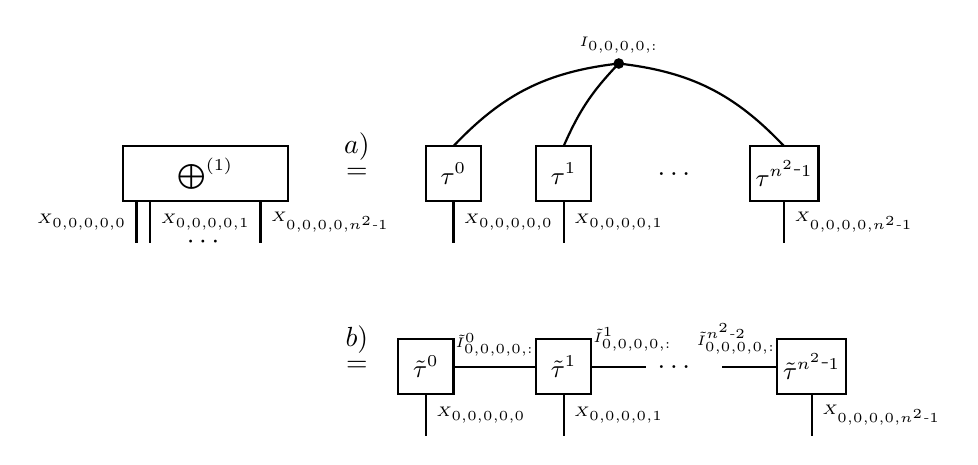
\begin{tikzpicture}[scale=0.35,thick]

                \draw (-6,-1) rectangle (-12,1);
                \node[anchor=center] (A) at (-9,0) {\corelabelsize $\woneoplus$};
                \draw (-11.5,-1)--(-11.5,-2.5) node[midway,left] {\colorlabelsize $\catvariableof{0,0,0,0,0}$};
                \draw (-11,-1)--(-11,-2.5) node[midway,right] {\colorlabelsize $\catvariableof{0,0,0,0,1}$};
                \node[anchor=center] (A) at (-9,-2.5) {$\cdots$};
                \draw (-7,-1)--(-7,-2.5) node[midway,right] {\colorlabelsize $\catvariableof{0,0,0,0,\sudokunum^2\shortminus 1}$};

                \node[anchor=center] (A) at (-3.5,1) {$a)$};
                \node[anchor=center] (A) at (-3.5,0) {$=$};

                \draw (-1,-1) rectangle (1,1);
                \node[anchor=center] (A) at (0,0) {\corelabelsize $\hypercoreof{0}$};
                \draw (0,-1)--(0,-2.5) node[midway,right] {\colorlabelsize $\catvariableof{0,0,0,0,0}$};

                \draw (3,-1) rectangle (5,1);
                \node[anchor=center] (A) at (4,0) {\corelabelsize $\hypercoreof{1}$};
                \draw (4,-1)--(4,-2.5) node[midway,right] {\colorlabelsize $\catvariableof{0,0,0,0,1}$};

                \node[anchor=center] (text) at (8,0) {$\hdots$};

                \draw (10.75,-1) rectangle (13.25,1);
                \node[anchor=center] (A) at (12,0) {\corelabelsize $\hypercoreof{\sudokunum^2\shortminus1}$};
                \draw (12,-1)--(12,-2.5) node[midway,right] {\colorlabelsize $\catvariableof{0,0,0,0,\sudokunum^2\shortminus1}$};

                \drawvariabledot{6}{4}
                \node[anchor=south] (text) at (6,4) {\colorlabelsize $\decvariableof{0,0,0,0,:}$};

                \draw (6,4) to[bend right= 20] (0,1);
                \draw (6,4) to[bend right= 10] (4,1);
                \draw (6,4) to[bend right= -20] (12,1);

                \begin{scope}[shift={(0,-7)}]
                    \node[anchor=center] (A) at (-3.5,1) {$b)$};
                    \node[anchor=center] (A) at (-3.5,0) {$=$};

                    \draw (-2,-1) rectangle (0,1);
                    \node[anchor=center] (A) at (-1,0) {\corelabelsize $\sechypercoreof{0}$};
                    \draw (-1,-1)--(-1,-2.5) node[midway,right] {\colorlabelsize $\catvariableof{0,0,0,0,0}$};

                    \draw (0,0) -- (3,0) node [midway,above] {\colorlabelsize $\secdecvariableof{0,0,0,0,:}^0$};

                    \draw (3,-1) rectangle (5,1);
                    \node[anchor=center] (A) at (4,0) {\corelabelsize $\sechypercoreof{1}$};
                    \draw (4,-1)--(4,-2.5) node[midway,right] {\colorlabelsize $\catvariableof{0,0,0,0,1}$};

                    \node[anchor=center] (text) at (6.5,1) {\colorlabelsize $\secdecvariableof{0,0,0,0,:}^{1}$};
                    \draw (5,0) -- (7,0); % node [midway,above] {\colorlabelsize $\secdecvariableof{0,0,0,0,:}^1$};

                    \node[anchor=center] (text) at (8,0) {$\hdots$};

                    \node[anchor=center] (text) at (10.25,1) {\colorlabelsize $\secdecvariableof{0,0,0,0,:}^{\sudokunum^2\shortminus2}$};
                    \draw (9.75,0) -- (11.75,0);

                    \draw (11.75,-1) rectangle (14.25,1);
                    \node[anchor=center] (A) at (13,0) {\corelabelsize $\sechypercoreof{\sudokunum^2\shortminus1}$};
                    \draw (13,-1)--(13,-2.5) node[midway,right] {\colorlabelsize $\catvariableof{0,0,0,0,\sudokunum^2\shortminus1}$};


                \end{scope}

            \end{tikzpicture}
        \end{center}
        \caption{Decomposition of the position constraint $\woneoplus$ at position $(r0,r1,c0,c1)=(0,0,0,0)$ into a) a $\cpformat$ decomposition with hidden variable $\decvariableof{0,0,0,0,:}$ and b) a $\ttformat$ decomposition with $d-1$ hidden variables $\decvariableof{0,0,0,0,:}^k, k\in[d-1]$.}
        \label{fig:sudokuDecomposition}
    \end{figure}

    Given evidence $\sudokustartevidence$ we denote the Sudoku Knowledge Base $\sudokukbof{\sudokunum,\sudokustartevidence}$.
    It is modelled as a tensor network on a hypergraph $\graphof{\mathrm{Sudoku},n}$ consisting of
    \begin{itemize}
        \item $\sudokunum^6+4\cdot \sudokunum^4$ nodes by $\sudokunum^6$ categorical variables $\catvariableof{(r0,r1,c0,c1,i)}$ and by $4\cdot \sudokunum^4$ decomposition variables to the constraints
        \item $5\cdot \sudokunum^6$ edges
        \begin{align*}
            \edges=
            \bigcup_{r0,r1,c0,c1\in[\sudokunum]}
            \big\{
            &\{\catvariableof{(r0,r1,c0,c1,i)}\},\{\catvariableof{(r0,r1,c0,c1,i)},\decvariableof{r0,r1,c0,c1,:}\},\{\catvariableof{(r0,r1,c0,c1,i)},\decvariableof{r0,r1,:,:,i}\},\\
            &\{\catvariableof{(r0,r1,c0,c1,i)},\decvariableof{:,:,c0,c1,i}\},
            \{\catvariableof{(r0,r1,c0,c1,i)},\decvariableof{r0,:,c0,:,i}\}\big\}
        \end{align*}
        We denote the decomposition variables to the position, row, column and square constraints by $\decvariableof{r0,r1,c0,c1,:},\decvariableof{r0,r1,:,:,i},\decvariableof{:,:,c0,c1,i}$ and $\decvariableof{r0,:,c0,:,i}$.
    \end{itemize}
    Each edge containing a decomposition variable is decorated by a matrix $\hypercoreofat{\catenumerator}{\catvariable,\decvariable}$ corresponding to a core in the $\cpformat$ decomposition of a constraint.
    Here, $\catenumerator$ is determined by the tuple $(r0,r1,c0,c1,i)$ and the type of the constraint (for example, for the variable $\catvariableof{(0,1,1,2,1)}$ and the row constraint $\decvariableof{(0,1,:,:,1)}$ we have $\catenumerator=1\cdot n + 2$.
    We further assign to each edge containing a single variable $\{\catvariableof{(r0,r1,c0,c1,i)}\}$ either the vector $\tbasisat{\catvariableof{(r0,r1,c0,c1,i)}}$ if $(r0,r1,c0,c1,i)\in \sudokustartevidence$ or the trivial vector $\onesat{\catvariableof{(r0,r1,c0,c1,i)}}$.
\end{example}

\subsection{Entailment Decision by Message-Passing}

% Infeasible contractions
Since contracting the whole tensor network is often infeasible, local contractions can be considered to decide entailment in some cases.
Here a local contraction describes the calculation of contractions along few closely connected tensors in the network.
Before presenting the resulting Constraint Propagation algorithm, we first show two important properties of local entailment motivating the procedure.

\begin{theorem}[Monotonicity of Propositional Logics]
    \label{the:monotonicityPL}
    If $\seckb\subset\kb$ and $\seckb\models\formula$ then also $\kb\models\formula$.
\end{theorem}
\begin{proof}
    Since $\seckb\models\formula$ it holds that $\contraction{\seckb[\shortcatvariables],\lnot\formula[\shortcatvariables]}=0$ and thus
    \begin{align*}
        \contractionof{\seckb[\shortcatvariables],\lnot\formula[\shortcatvariables]}{\shortcatvariables}=\zerosat{\shortcatvariables} \, .
    \end{align*}
    Denoting by $\kb/\seckb$ the conjunctions of formulas in $\kb$ not in $\seckb$, we have
    \begin{align*}
        \contraction{\kbwith,\lnot\formulawith}
        &= \contraction{(\kb/\seckb)[\shortcatvariables],\seckb[\shortcatvariables],\lnot\formulawith} \\
        &= \contraction{(\kb/\seckb)[\shortcatvariables],\contractionof{\seckb[\shortcatvariables],\lnot\formulawith}{\shortcatvariables}} \\
        &= \contraction{(\kb/\seckb)[\shortcatvariables],\zerosat{\shortcatvariables}} \\
        &= 0 \, .
    \end{align*}
\end{proof}
To decide entailment, we can therefore investigate entailment on smaller parts of the knowledge base.
This is sound by the above theorem, but not complete, since it can happen that no smaller part of the knowledge base entails the formula, but the whole knowledge base does.
We can futhermore add entailed formulas to the knowledge base without the latter, as we show next.

\begin{theorem}[Invariance of adding Entailed Formulas]
    \label{the:addingEntailed}
    If and only if $\kb\models\formula$ we have
    \begin{align*}
        \kbwith
        = \contractionof{\kbwith,\formulawith}{\shortcatvariables} \, .
    \end{align*}
\end{theorem}
\begin{proof}
    We use that $\formulawith+\lnot\formulawith=\onesat{\shortcatvariables}$ and thus
    \begin{align*}
        \kbwith
        &= \contractionof{\kbwith,(\formulawith+\lnot\formulawith)}{\shortcatvariables} \\
        &= \contractionof{\kbwith,\formulawith}{\shortcatvariables}  + \contractionof{\kbwith,\lnot\formulawith}{\shortcatvariables}  \\
        %&= \contractionof{\kbwith,\formulawith}{\shortcatvariables} \, .
    \end{align*}
    Since $\contractionof{\kbwith,\lnot\formulawith}{\shortcatvariables}$ is boolean, we thus have that
    \begin{align*}
        \kbwith=\contractionof{\kbwith,\formulawith}{\shortcatvariables}
    \end{align*}
    if and only if $\contraction{\kbwith,\lnot\formulawith}=0$, that is $\kb\models\formula$.
\end{proof}

% Interpreting entailment
The mechanism of \theref{the:addingEntailed} provides us with a mean to store entailment information in small order auxiliary tensors.
%Adding deduced statements to a knowledge base does not change the knowledge base as a tensor, but one can exploit it in smaller contractions.
% Constraint Propagation
One way to exploit this accessibility of local entailment information are message passing schemes similar to \algoref{alg:treeBeliefPropagation} propagating the information.
This approach decides local entailment by iteratively adding entailed formulas to the knowledge base and checking further entailment on neighbored tensors of the knowledge base.
Since for entailment decisions the support of the contractions is sufficient, we can apply non-zero indicators before sending contraction messages.
We then schedule new messages in the direction $(\sedge,\redge)$, once the support of a message received at $\sedge$ has been changed.
Note that such a scheduling system is guaranteed to converge, since there can only be a finite number of message changes.
We further directly reduce the computation of messages to their support and call the resulting \algoref{alg:constraintPropagation} Constraint Propagation.

\begin{algorithm}[hbt!]
    \caption{Constraint Propagation}\label{alg:constraintPropagation}
    \begin{algorithmic}
        \Require Tensor network $\extnet$ on a hypergraph $\graph$
        \Ensure Messages $\{\messagewith\wcols(\secsedge,\sedge)\in\dirovedges\}$ containing entailment statements
        \iosepline
        \State Initialize a queue $\scheduler = \dirovedges$ of message directions
        \State Initialize messages $\messagewith = \onesat{\catvariableof{\sedge\cap\redge}}$ for $(\sedge,\redge)\in\dirovedges$
        \While{$\scheduler$ not empty}
            \State Pop a $(\sedge,\redge)$ pair from $\scheduler$
            \State Update the message
            \begin{align*}
                \messagewith
                = \nonzeroof{\contractionof{\{\hypercoreofat{\sedge}{\catvariableof{\sedge}}\}
                    \cup \{\mesfromtoat{\secsedge}{\sedge}{\catvariableof{\secsedge\cap\sedge}} \wcols (\secsedge,\sedge)\in\dirovedges \ncond \secsedge\neq \redge\}
                }{\catvariableof{\sedge\cap \redge}}}
            \end{align*}
            \If{$\hypercoreat{\catvariableof{\sedge\cap \redge}}\neq\messagewith$}
                \State Update the message: $\messagewith\coloneqq\hypercoreat{\catvariableof{\sedge\cap \redge}}$
                \State Add $\scheduler = \scheduler \cup \{(\redge,\secsedge) \wcols (\redge,\secsedge)\in\dirovedges\}$ % Clear?
            \EndIf
        \EndWhile
        \State \Return Messages $\{\messagewith\wcols(\secsedge,\sedge)\in\dirovedges\}$
    \end{algorithmic}
\end{algorithm}

\begin{theorem}
    \label{the:constraintPropagationSoundness}
    All messages during constraint propagation are sound, that is for all $(\sedge,\redge)\in\dirovedges$ it holds that
    \begin{align*}
        \nonzeroof{\contractionof{\extnet}{\catvariableof{\sedge\cap\redge}}} \prec \messagewith \, .
    \end{align*}
\end{theorem}
\begin{proof}
    We show this theorem by induction over the $\mathrm{While}$ loop of \algoref{alg:constraintPropagation}.
    At the first iteration, we have for all messages $\messagewith=\onesat{\catvariableof{\sedge\cap\redge}}$ and thus
    \begin{align}
        \label{eq:nzMessageAddingEquivalence}
        \extnet = \contractionof{\{\extnet\}\cup\{\messagewith\wcols(\sedge,\redge)\in\dirovedges\}}{\nodevariables} \, .
    \end{align}
    By \theref{the:monotonicityPL} we then have for the first message send along the pair $(\sedge,\redge)$ that
    \begin{align*}
        \nonzeroof{\contractionof{\extnet}{\catvariableof{\sedge\cap\redge}}} \prec
        &\nonzeroof{\contractionof{\{\hypercoreofat{\sedge}{\catvariableof{\sedge}}\}
            \cup \{\mesfromtoat{\secsedge}{\sedge}{\catvariableof{\secsedge\cap\sedge}} \wcols (\secsedge,\sedge)\in\dirovedges \ncond \secsedge\neq \redge\}
        }{\catvariableof{\sedge\cap \redge}}} \\
        &= \messagewith \, .
    \end{align*}

    Let us now assume that at an arbitrary state of the algorithm the inequality holds for all previous sent messages.
    By \theref{the:addingEntailed} we can add contract the messages on the tensor network without changing it, and \eqref{eq:nzMessageAddingEquivalence} thus still holds.
    We then conclude with \theref{the:monotonicityPL} that the claimed property also holds for the new message.
\end{proof}

\begin{example}[Constraint Propagation for the Sudoku of \exaref{exa:sudokuEntailment}]
    \label{exa:sudokuMessagePassing}
    We iteratively solve a Sudoku puzzle by determining a possible value based on neighboring cells, rows and squares (using \theref{the:monotonicityPL}) and adding to our knowledge (using \theref{the:addingEntailed}).
    For example, consider the following $\sudokunum=2$ Sudoku puzzle, where a first entailment step uses only the knowledge of the rules and the \textcolor{\concolor}{blue} cells to determine the value $3$ in the first square:
    \begin{center}
        \begin{sudoku4x4}
            \matrix[sudokumatrix] (M) at (0,0) {
                1 & \ & \textcolor{\concolor}{3} & 2 \\
                \ & \textcolor{\concolor}{2} & \  & \  \\
                \ & \ & 4 & \ \\
                4 & 3 &  \ & \  \\
            };
            \draw[thick]([yshift=9.5pt,xshift=-0.6pt]M-1-2.east) -- ([yshift=-9.5pt,xshift=-0.6pt]M-4-2.east);
            \draw[thick]([xshift=-9.5pt,yshift=0.6pt]M-2-1.south) -- ([xshift=9.5pt,yshift=0.6pt]M-2-4.south);

            \node[anchor=center] (ist) at (1.75,0) {$=$};

            \matrix[sudokumatrix] (M) at (3.5,0) {
                1 & \ & 3 & 2 \\
                \textcolor{\probcolor}{3} & 2 & \  & \  \\
                \ & \ & 4 & \ \\
                4 & 3 &  \ & \  \\
            };
            \draw[thick]([yshift=9.5pt,xshift=-0.6pt]M-1-2.east) -- ([yshift=-9.5pt,xshift=-0.6pt]M-4-2.east);
            \draw[thick]([xshift=-9.5pt,yshift=0.6pt]M-2-1.south) -- ([xshift=9.5pt,yshift=0.6pt]M-2-4.south);

            \node[anchor=center] (ist) at (6.25,0) {$= \quad \ldots \quad =$};

            \matrix[sudokumatrix] (M) at (9,0) {
                1 & \textcolor{\probcolor}{4} & 3 & 2 \\
                \textcolor{\probcolor}{3} & 2 & \textcolor{\probcolor}{1} & \textcolor{\probcolor}{4}  \\
                \textcolor{\probcolor}{2} & \textcolor{\probcolor}{1} & 4 & \textcolor{\probcolor}{3} \\
                4 & 3 & \textcolor{\probcolor}{2} & \textcolor{\probcolor}{1}  \\
            };
            \draw[thick]([yshift=9.5pt,xshift=-0.6pt]M-1-2.east) -- ([yshift=-9.5pt,xshift=-0.6pt]M-4-2.east);
            \draw[thick]([xshift=-9.5pt,yshift=0.6pt]M-2-1.south) -- ([xshift=9.5pt,yshift=0.6pt]M-2-4.south);
        \end{sudoku4x4}
    \end{center}

    To illustrate the first reasoning step of assigning $\textcolor{\probcolor}{\catvariableof{0,1,0,0,2}}$, we make the following entailment steps applying \theref{the:monotonicityPL}.
    We also depict in \figref{fig:contractionPropagationSudoku} the corresponding messages in the Constraint Propagation Algorithm on the hypergraph $\graph^{\mathrm{Sudoku},n}$.
    \begin{itemize}
        \item From $\textcolor{\concolor}{\catvariableof{0,1,0,1,1}}$ (i.e. the $2$ in the cell $(0,1,0,1)$) and the Sudoku rule that at the cell $(0,1,0,1)$ exactly one number is assigned, we get
        \begin{align*}
            \left( \woneoplus_{i\in[\sudokunum^2]} \catvariableof{0,1,0,1,i} \right) \land \textcolor{\concolor}{\catvariableof{0,1,0,1,1}} \models \lnot\catvariableof{0,1,0,1,2} \, ,
        \end{align*}
        That is, that the number $3$ is not in the cell $(0,1,0,1)$.
        This entailment step is performed by three consecutive messages (see $\messagesymbol^{(0,[3])}$ in \figref{fig:contractionPropagationSudoku}) along the directions %involving decomposition cores of the position constraint in the position $(r_0,r_1,c_0,c_1)=(0,0,0,0)$.
        \begin{align*}
        (\sedge,\redge)
            \in \big[&(\{\catvariableof{0,1,0,1,1}\},\{\catvariableof{0,1,0,1,1},\decvariableof{0,1,0,1,:}\}),
                (\{\catvariableof{0,1,0,1,1},\decvariableof{0,1,0,1,:}\},\{\catvariableof{0,1,0,1,2},\decvariableof{0,1,0,1,:}\}), \\
                &(\{\catvariableof{0,1,0,1,2},\decvariableof{0,1,0,1,:}\},\{\catvariableof{0,1,0,1,2},\decvariableof{0,:,0,:,2}\})\big] \, .
        \end{align*}
        Intuitively, the messages commmunicate to the square constraint $\decvariableof{0,:,0,:,2}$, that by the position constraint $\decvariableof{0,1,0,1,:}$ the variable $3$ cannot be assigned at $(0,1,0,1)$.
        %This entailment step is performed by two consecutive messages along the directions $(\catvariableof{0,1,0,1,1},\decvariableof{0,1,0,1,:})$ and $(\decvariableof{0,1,0,1,:},\catvariableof{0,1,0,1,2})$.
        \item From $\textcolor{\concolor}{\catvariableof{0,0,1,0,2}}$ (i.e. the $3$ in the cell $(0,0,1,0)$) and the Sudoku rule that at the row $(0,0)$ exactly one number is assigned, we get
        \begin{align*}
            \left( \woneoplus_{c0,c1\in[\sudokunum]} \catvariableof{0,0,c0,c1,2} \right) \land \textcolor{\concolor}{\catvariableof{0,0,1,0,2}} \models \lnot\catvariableof{0,0,0,0,2}\land \lnot\catvariableof{0,0,0,1,2} \, ,
        \end{align*}
        meaning that the number $3$ is neither in the cell $(0,0,0,0)$ nor in $(0,0,0,1)$.
        This entailment step is performed by five consecutive messages (see $\messagesymbol^{(1,[5])}$ in \figref{fig:contractionPropagationSudoku}) along the directions
        %This entailment step is performed by three consecutive messages along the directions $(\catvariableof{0,0,1,0,2},\decvariableof{0,0,:,:,2})$, $(\decvariableof{0,0,:,:,2},\catvariableof{0,0,0,0,2})$ and $(\decvariableof{0,0,:,:,2},\catvariableof{0,0,0,1,2})$.
        \begin{align*}
        (\sedge,\redge)
            \in \big[
            &(\{\catvariableof{0,0,1,0,2}\},\{\catvariableof{0,0,1,0,2},\decvariableof{0,0,:,:,2}\}),
                (\{\catvariableof{0,0,1,0,2},\decvariableof{0,0,:,:,2}\},\{\catvariableof{0,0,0,0,2},\decvariableof{0,0,:,:,2}\}), \\
                &(\{\catvariableof{0,0,1,0,2},\decvariableof{0,0,:,:,2}\},\{\catvariableof{0,0,0,1,2},\decvariableof{0,0,:,:,2}\}),
                (\{\catvariableof{0,0,0,0,2},\decvariableof{0,0,:,:,2}\},\{\catvariableof{0,0,0,0,2},\decvariableof{0,:,0,:,2}\}) \\
                &(\{\catvariableof{0,0,0,1,2},\decvariableof{0,0,:,:,2}\},\{\catvariableof{0,0,0,1,2},\decvariableof{0,:,0,:,2}\})
                \big] \, .
        \end{align*}
        The messages communicate that based on the decomposition cores of the constraint to the number $i=3$ in the first row $(r_0,r_1)=(0,0)$, the number $3$ cannot be assigned at $(0,0,0,0)$ and $(0,0,0,1)$.
    \end{itemize}
    We add these formulas to our knowledge base (justified by \theref{the:addingEntailed}) and use the rule that $3$ appears exactly once in the first square
    \begin{align*}
        &\left( \woneoplus_{r1,c1\in[\sudokunum]} \catvariableof{0,r1,0,c1,2} \right)
        \land (\lnot\catvariableof{0,1,0,1,2})
        \land (\lnot\catvariableof{0,0,0,0,2}\land \lnot\catvariableof{0,0,0,1,2})
        \models \textcolor{\probcolor}{\catvariableof{0,1,0,0,2}} \, .
    \end{align*}
    We hence conclude that the number $3$ must be in the cell $(0,1,0,0)$.
    This information is also included in the updated knowledge base for further reasoning steps.
    This last entailment step is performed by four consecutive messages (see $\messagesymbol^{(2,[4])}$ in \figref{fig:contractionPropagationSudoku}) along the directions
    \begin{align*}
    (\sedge,\redge)
        \in \big[
            &(\{\catvariableof{0,1,0,1,2},\decvariableof{0,:,0,:,2}\},\{\catvariableof{0,1,0,0,2},\decvariableof{0,:,0,:,2}\}),
            (\{\catvariableof{0,0,0,1,2},\decvariableof{0,:,0,:,2}\},\{\catvariableof{0,1,0,0,2},\decvariableof{0,:,0,:,2}\}), \\
            &(\{\catvariableof{0,0,1,0,2},\decvariableof{0,:,0,:,2}\},\{\catvariableof{0,1,0,0,2},\decvariableof{0,:,0,:,2}\}),
            (\{\catvariableof{0,1,0,0,2},\decvariableof{0,:,0,:,2}\},\{\catvariableof{0,1,0,0,2}\})\big]
    \end{align*}
    The first three messages communicate that the $3$ is not possible in positions $(0,1,0,1),(0,0,0,1)$ and $(0,0,1,0)$ and the fourth message concludes that the $3$ then has to be at position $(0,1,0,0)$.

    %% Further reasoning steps
    We now iteratively apply similar reasoning steps and store the entailed variables in \textcolor{\probcolor}{$E^{\mathrm{entailed}}$} until we arrive at the right side of the above sketch.
    \begin{align*}
        \sudokukbof{2} \land \left(\bigwedge_{(r_0,r_1,c_0,c_1,i)\in \sudokustartevidence} \catvariableof{r0,r1,c0,c1,i} \right)
        \models \textcolor{\probcolor}{\left(\bigwedge_{(r_0,r_1,c_0,c_1,i)\in E^{\mathrm{entailed}}} \catvariableof{r0,r1,c0,c1,i} \right)} \, .
    \end{align*}
    Since all Sudoku rules are satisfied in the final assignment and to each cell $(r_0,r_1,c_0,c_1)$ we found exactly one $i\in[\sudokunum^2]$ such that $(r_0,r_1,c_0,c_1,i)\in \sudokustartevidence\cup\textcolor{\probcolor}{E^{\mathrm{entailed}}}$, there is a unique solution of the puzzle and we conclude that
    \begin{align*}
        &\sudokukbof{2} \land \left(\bigwedge_{(r_0,r_1,c_0,c_1,i)\in \sudokustartevidence} \catvariableof{r0,r1,c0,c1,i} \right) \\
        &\quad= \left(\bigwedge_{(r_0,r_1,c_0,c_1,i)\in \sudokustartevidence} \catvariableof{r0,r1,c0,c1,i} \right)
        \land \textcolor{\probcolor}{\left(\bigwedge_{(r_0,r_1,c_0,c_1,i)\in E^{\mathrm{entailed}}} \catvariableof{r0,r1,c0,c1,i} \right)} \, .
    \end{align*}
\end{example}

\begin{figure}[t]
    \begin{center}
        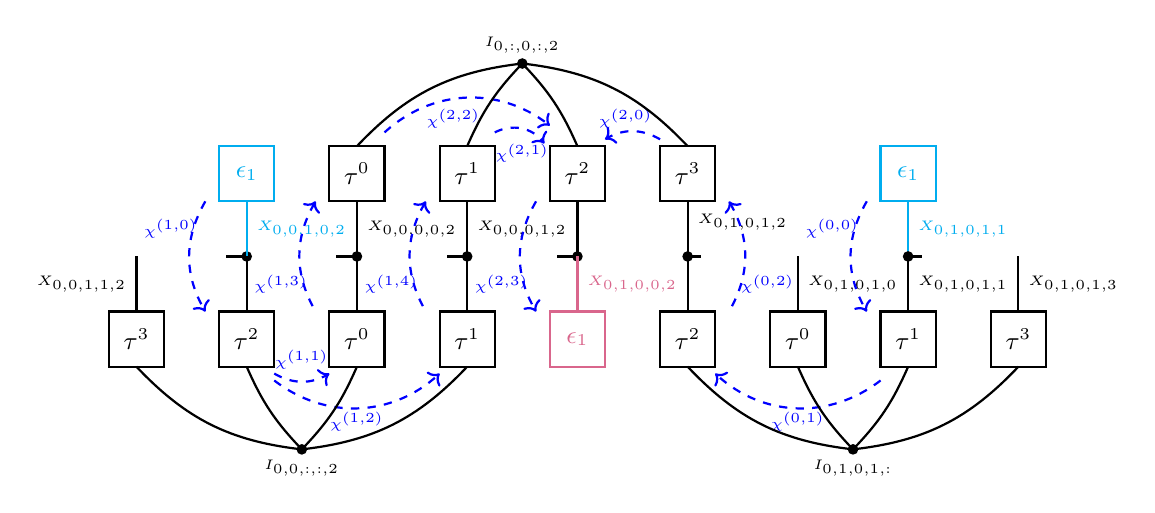
\begin{tikzpicture}[scale=0.35,thick]

            %% I 0:0:2 constraint (3 is in the 00 square)
            \draw (-1,-1) rectangle (1,1);
            \node[anchor=center] (A) at (0,0) {\corelabelsize $\hypercoreof{0}$};
            \draw (0,-1)--(0,-3) node[midway,right] {\colorlabelsize $\catvariableof{0,0,0,0,2}$};

            \draw (3,-1) rectangle (5,1);
            \node[anchor=center] (A) at (4,0) {\corelabelsize $\hypercoreof{1}$};
            \draw (4,-1)--(4,-3) node[midway,right] {\colorlabelsize $\catvariableof{0,0,0,1,2}$};

            \draw (7,-1) rectangle (9,1);
            \node[anchor=center] (A) at (8,0) {\corelabelsize $\hypercoreof{2}$};
            \draw (8,-1)--(8,-3); % node[midway,right] {\colorlabelsize $\catvariableof{0,1,0,0,2}$};

            \drawvariabledot{8}{-3}
            \draw (8,-3) -- (7.25,-3);
            \draw[\probcolor] (7,-5) rectangle (9,-7);
            \node[anchor=center, \probcolor] (A) at (8,-6) {\corelabelsize $\tbasis$};
            \draw[\probcolor] (8,-5)--(8,-3) node[midway,right] {\colorlabelsize $\catvariableof{0,1,0,0,2}$};

            \draw[\newmessagecolor,dashed, ->] (6.5,-1) to [bend right = 30] (6.5,-5);
            \node[\newmessagecolor,anchor=center] (A) at (5.25,-4) {\colorlabelsize $\messagesymbol^{(2,3)}$};

            \draw[\newmessagecolor,dashed, ->] (11,1.25) to [bend right = 30] (9,1.25);
            \node[\newmessagecolor,anchor=center] (A) at (9.75,2) {\colorlabelsize $\messagesymbol^{(2,0)}$};

            \draw[\newmessagecolor,dashed, ->] (5,1.5) to [bend right = -40] (6.8,1.1);
            \node[\newmessagecolor,anchor=center] (A) at (6,0.75) {\colorlabelsize $\messagesymbol^{(2,1)}$};

            \draw[\newmessagecolor,dashed, ->] (1,1.5) to [bend right = -40] (7,1.75);
            \node[\newmessagecolor,anchor=center] (A) at (3.5,2) {\colorlabelsize $\messagesymbol^{(2,2)}$};


            \draw (11,-1) rectangle (13,1);
            \node[anchor=center] (A) at (12,0) {\corelabelsize $\hypercoreof{3}$};
            \draw (12,-1)--(12,-2.5) node[midway,right] {\colorlabelsize $\catvariableof{0,1,0,1,2}$};

            \drawvariabledot{6}{4}
            \node[anchor=south] (text) at (6,4) {\colorlabelsize $\decvariableof{0,:,0,:,2}$};

            \draw (6,4) to[bend right= 20] (0,1);
            \draw (6,4) to[bend right= 10] (4,1);
            \draw (6,4) to[bend right= -10] (8,1);
            \draw (6,4) to[bend right= -20] (12,1);


            %% I 00::2 constraint (3 in the first row)
            \draw (3,-7) rectangle (5,-5);
            \node[anchor=center] (A) at (4,-6) {\corelabelsize $\hypercoreof{1}$};
            \drawvariabledot{4}{-3}
            \draw (4,-3) -- (3.25,-3);
            \draw (4,-5)--(4,-1);

            \draw (-1,-7) rectangle (1,-5);
            \node[anchor=center] (A) at (0,-6) {\corelabelsize $\hypercoreof{0}$};
            \drawvariabledot{0}{-3}
            \draw (0,-3) -- (-0.75,-3);
            \draw (0,-5)--(0,-1);

            \draw (-5,-7) rectangle (-3,-5);
            \node[anchor=center] (A) at (-4,-6) {\corelabelsize $\hypercoreof{2}$};
            \draw (-4,-5)--(-4,-3);

            \drawvariabledot{-4}{-3}
            \draw (-4,-3) -- (-4.75,-3);

            \draw[\concolor] (-5,-1) rectangle (-3,1);
            \node[anchor=center, \concolor] (A) at (-4,0) {\corelabelsize $\tbasis$};
            \draw[\concolor] (-4,-1)--(-4,-3) node[midway,right] {\colorlabelsize $\catvariableof{0,0,1,0,2}$};

            %% Messages from 3 in row 0,0
            \draw[\newmessagecolor,dashed, ->] (-5.5,-1) to [bend right = 30] (-5.5,-5);
            \node[\newmessagecolor,anchor=center] (A) at (-6.75,-2) {\colorlabelsize $\messagesymbol^{(1,0)}$};

            \draw[\newmessagecolor,dashed, ->] (-3,-7.25) to [bend right = 30] (-1,-7.25);
            \node[\newmessagecolor,anchor=center] (A) at (-2,-6.75) {\colorlabelsize $\messagesymbol^{(1,1)}$};

            \draw[\newmessagecolor,dashed, ->] (-3,-7.5) to [bend right = 40] (3,-7.25);
            \node[\newmessagecolor,anchor=center] (A) at (0,-9) {\colorlabelsize $\messagesymbol^{(1,2)}$};

            \draw[\newmessagecolor,dashed, <-] (-1.5,-1) to [bend right = 30] (-1.5,-5);
            \node[\newmessagecolor,anchor=center] (A) at (-2.75,-4) {\colorlabelsize $\messagesymbol^{(1,3)}$};

            \draw[\newmessagecolor,dashed, <-] (2.5,-1) to [bend right = 30] (2.5,-5);
            \node[\newmessagecolor,anchor=center] (A) at (1.25,-4) {\colorlabelsize $\messagesymbol^{(1,4)}$};

            \draw (-9,-7) rectangle (-7,-5);
            \node[anchor=center] (A) at (-8,-6) {\corelabelsize $\hypercoreof{3}$};
            \draw (-8,-5)--(-8,-3) node[midway,left] {\colorlabelsize $\catvariableof{0,0,1,1,2}$};

            \drawvariabledot{-2}{-10}
            \node[anchor=north] (text) at (-2,-10) {\colorlabelsize $\decvariableof{0,0,:,:,2}$};

            \draw (-2,-10) to[bend right= -20] (-8,-7);
            \draw (-2,-10) to[bend right= -10] (-4,-7);
            \draw (-2,-10) to[bend right= 10] (0,-7);
            \draw (-2,-10) to[bend right= 20] (4,-7);

            % I 0001: (position 0001)
            \draw (11,-7) rectangle (13,-5);
            \node[anchor=center] (A) at (12,-6) {\corelabelsize $\hypercoreof{2}$};
            \draw (12,-5)--(12,-2.5);

            \drawvariabledot{12}{-3}
            \draw (12,-3) -- (12.5,-3);

            \draw (15,-7) rectangle (17,-5);
            \node[anchor=center] (A) at (16,-6) {\corelabelsize $\hypercoreof{0}$};
            \draw (16,-5)--(16,-3) node[midway,right] {\colorlabelsize $\catvariableof{0,1,0,1,0}$};

            \draw (19,-7) rectangle (21,-5);
            \node[anchor=center] (A) at (20,-6) {\corelabelsize $\hypercoreof{1}$};
            \draw (20,-5)--(20,-3) node[midway,right] {\colorlabelsize $\catvariableof{0,1,0,1,1}$};

            \draw[\concolor] (19,-1) rectangle (21,1);
            \node[anchor=center, \concolor] (A) at (20,0) {\corelabelsize $\tbasis$};
            \draw[\concolor] (20,-1)--(20,-3) node[midway,right] {\colorlabelsize $\catvariableof{0,1,0,1,1}$};

            \drawvariabledot{20}{-3}
            \draw (20,-3) -- (20.5,-3);

            %% Messages from 2 at position 2,2,2,2
            \draw[\newmessagecolor,dashed, ->] (18.5,-1) to [bend right = 30] (18.5,-5);
            \node[\newmessagecolor,anchor=center] (A) at (17.25,-2) {\colorlabelsize $\messagesymbol^{(0,0)}$};

            \draw[\newmessagecolor,dashed, ->] (19,-7.5) to [bend right = -40] (13,-7.25);
            \node[\newmessagecolor,anchor=center] (A) at (16,-9) {\colorlabelsize $\messagesymbol^{(0,1)}$};

            \draw[\newmessagecolor,dashed, <-] (13.5,-1) to [bend right = -30] (13.5,-5);
            \node[\newmessagecolor,anchor=center] (A) at (14.9,-4) {\colorlabelsize $\messagesymbol^{(0,2)}$};

            \draw (23,-7) rectangle (25,-5);
            \node[anchor=center] (A) at (24,-6) {\corelabelsize $\hypercoreof{3}$};
            \draw (24,-5)--(24,-3) node[midway,right] {\colorlabelsize $\catvariableof{0,1,0,1,3}$};

            \drawvariabledot{18}{-10}
            \node[anchor=north] (text) at (18,-10) {\colorlabelsize $\decvariableof{0,1,0,1,:}$};

            \draw (18,-10) to[bend right= -20] (12,-7);
            \draw (18,-10) to[bend right= -10] (16,-7);
            \draw (18,-10) to[bend right= 10] (20,-7);
            \draw (18,-10) to[bend right= 20] (24,-7);

        \end{tikzpicture}
    \end{center}
    \caption{
        The tensor network decomposition of $3$ out of $4\cdot2^2=64$ rules in the $2^2\times2^2$ Sudoku knowledge base (see \exaref{exa:sudokuDecomposition}),  namely to the number $3$ appearing once in the $(0,0)$-square (top), the number $3$ appearing once in the $(0,0)$-row (bottom left) and a unique number appearing at the $(0,1,0,1)$-position (bottom right).
        The evidence of the number $3$ already being assigned at the position $(0,0,1,0)$ is sketched by a basis vector $\textcolor{\concolor}{\tbasis}$ on the left side, and the number $2$ assigned at position $(0,1,0,1)$ analogously on the right side.
        During Constraint Propagation \algoref{alg:constraintPropagation} on the hypergraph of Sudoku rules and evidence (see \exaref{exa:sudokuMessagePassing}), this evidence is in three epochs of messages propagated to the constraints by partial entailment steps and imply that $\textcolor{\probcolor}{\catvariableof{0,1,0,0,2}}$ is true, i.e. that at the position $(0,1,0,0)$ the number $3$ needs to be assigned.
        We depict the messages between the cores by dashed lines labeled by $\messagesymbol^{(0,[3])},\messagesymbol^{(1,[5])}$ and $\messagesymbol^{(2,[4])}$ and provide further interpretation in \exaref{exa:sudokuMessagePassing}.
    }\label{fig:contractionPropagationSudoku}
\end{figure}


\section{\HybridLogicNetworks{}}\label{sec:hln}

Let us now exploit the common formulation of logical formulas and probabilistic models in \CompActNets{} to define hybrid models that combine both aspects.
We call \CompActNets{} \HybridLogicNetworks{} in the special case of Boolean statistics $\sstat$ and elementary activations.

\subsection{Parametrization}

We first introduce \HybridLogicNetworks{}, which can be regarded as a unification of logical and probabilistic models.

\begin{definition}[\HybridLogicNetwork{} (HLN)]
    \label{def:hybridLogicNetwork}
    Given a Boolean statistic $\hlnstat$, we call any element of $\elrealizabledistsof{\hlnstat}$ a \HybridLogicNetwork{}.
    The extended canonical parameter set for $\hlnstat$ is the set
    \begin{align*}
        \hybridparamset\coloneqq
        \{\hardparam\wcols \hardlegset\subset[\seldim]\ncond \headindexof{\hardlegset}\in\bigtimes_{\selindex\in\hardlegset}[2]\} \times \parspace \, .
    \end{align*}
    For each \HybridLogicNetwork{} $\hlnwith$, we can associate a tuple $\hybridparam$ consisting of a subset $\hardlegset\subset[\seldim]$, a tuple $\headindexof{\hardlegset}\in\bigtimes_{\selindex\in\hardlegset}[2]$, and $\canparamwithin$ such that
    \begin{align*}
        \hlnwith
        = \normalizationof{\hlnstatccwith,\paracttensorwith}{\shortcatvariables}
    \end{align*}
    where the activation core is
    \begin{align*}
        \paracttensorwith = \contractionof{\softacttensorwith,\hardacttensorwith}{\headvariables} \, .
    \end{align*}
\end{definition}

%% Parametrization explanation
We notice that the parametrization by $\hybridparamset$ is one-to-one for any non-vanishing elementary activation tensor up to a scalar factor.
Given an arbitrary elementary activation tensor $\bigotimes_{\selindexin}\acttensorlegwith$, we can always find a corresponding tuple in $\hybridparamset$ by choosing\footnote{Here $\nonzeroof{\cdot}$ is the indicator of non-zero entries acting coordinatewise and $\onesat{\headvariableof{\selindex}}$ is the vector $[1,1]^T$.}
\begin{align*}
    \hardlegset = \{\selindex \wcols \nonzeroof{\acttensorlegwith}\neq\onesat{\headvariableof{\selindex}}\} \, ,
\end{align*}
further for all $\selindex\in\hardlegset$
\begin{align*}
    \headindexof{\selindex}
    = \begin{cases}
          0 & \ifspace \nonzeroof{\acttensorlegwith} = \onehotmapofat{0}{\headvariableof{\selindex}} \\
          1 & \ifspace \nonzeroof{\acttensorlegwith} = \onehotmapofat{1}{\headvariableof{\selindex}} \,
    \end{cases}
\end{align*}
and a parameter vector $\canparamwithin$ defined for all $\selindexin$ as
\begin{align*}
    \canparamat{\indexedselvariable} =
    \begin{cases}
        0 & \ifspace \selindex\in\hardlegset \\
        \lnof{\frac{\acttensorlegat{\headvariableof{\selindex}=1}}{\acttensorlegat{\headvariableof{\selindex}=0}}}
        & \ifspace \selindex\notin\hardlegset \, .
    \end{cases}
\end{align*}
Then we have by construction that there is $\lambda>0$ with
\begin{align*}
    \bigotimes_{\selindexin}\acttensorlegwith
    = \lambda \cdot \paracttensorwith \, .
\end{align*}

Let us demonstrate the utility of \HybridLogicNetworks{} with an example from accounting.

\begin{example}[\HybridLogicNetwork{} for a Toy Accounting Model]
    \label{exa:hlnAccountingRep}

    Let us consider a system of three variables $A1$ Account 1 is booked, $A2$ Account 2 is booked, $F$ a feature on an invoice.
    We respect two rules
    \begin{itemize}
        \item \textcolor{\concolor}{Exactly one account must be booked.}
        \item \textcolor{\probcolor}{If feature $\mathrm{F}$ is present on the invoice, the account $\mathrm{A1}$ is typically booked.}
    \end{itemize}
    We formalize this with the statistic
    \begin{align*}
        \hlnstat = (\catvariableof{A1} \oplus \catvariableof{A2}, \catvariableof{F}\Rightarrow \catvariableof{A1})\, .
    \end{align*}
    While the first formula is a hard feature, the second is soft since prone to exceptions.
    We parameterize the first output of the statistic with the hard parameters by setting the set of indices to be initialized with hard logic $A = \{0\}$ and the corresponding initialization $y_0 = 1$ meaning, that the first output of the statistic has to be true for the input to have positive probability.
% \begin{align*}
%     \hardlegset = \{0\} \quad, \quad \headindexof{\hardlegset} = 1.
% \end{align*}
    Then "hard logic activation tensor", should be indifferent to the second part of the statistic, and only impose rules on the first part, leading to
    \begin{align*}
        \textcolor{\concolor}{\kappa^{(A,y_A)}[Y_0,Y_1]} =
        \onehotmapofat{\headindexof{0}}{\headvariableof{0}} \otimes
        \onesat{\headvariableof{1}}
        =\begin{bmatrix}
             0 \\
             1
        \end{bmatrix} \otimes \begin{bmatrix}
                                  1\\1
        \end{bmatrix}.
    \end{align*}
    Since the first feature is hard, the "soft logic activation tensor" should be invariant under the first coordinate of the canonical parameter and we set $\canparamat{\selvariable=0}=0$. We choose the soft parameters as $\theta[L] = [0,\theta[L=1]]^\intercal$ to achieve
    \begin{align*}
        \textcolor{\probcolor}{\alpha^\theta[Y_0,Y_1]} &= \alpha^{0,0}\left[Y_0\right]\otimes \alpha^{1,\theta[L=1]}\left[Y_1\right] = \begin{bmatrix}
                                                                                                                                           1\\1
        \end{bmatrix}\otimes \begin{bmatrix}
                                 1\\ \expof{\canparamat{\selvariable=1}}
        \end{bmatrix}.
        % \\
        % \canparamat{\selvariable} 
        % &= \begin{bmatrix}
        %     0 \\
        %     \canparamat{\selvariable=1}
        % \end{bmatrix} \, .
    \end{align*}
    The activation tensor of the hybrid network then has the from
    \begin{align*}
        \paracttensor[{\headvariableof{0},\headvariableof{1}}]
        = \begin{bmatrix}
              0 \\ 1
        \end{bmatrix}
        \otimes
        \begin{bmatrix}
            1 \\ \expof{\canparamat{\selvariable=1}}
        \end{bmatrix}.
    \end{align*}

    We get a tensor network representation of the \HybridLogicNetwork{} representing the toy accounting example, before normalization to a distribution
    \begin{center}
        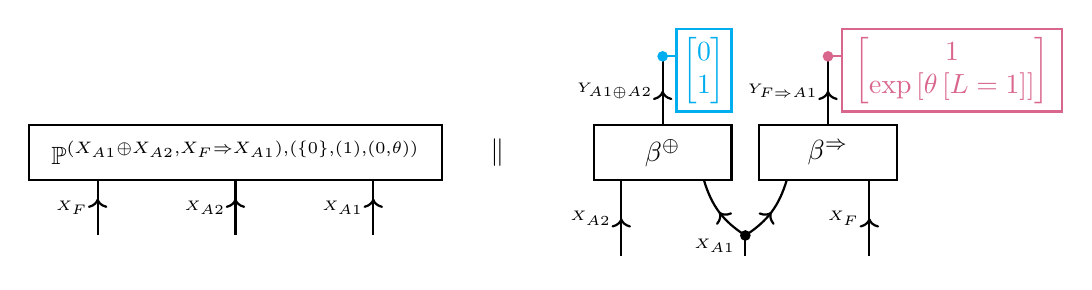
\begin{tikzpicture}[scale=0.35, thick, yscale=-1, xscale=-1] % , baseline = -3.5pt

            \begin{scope}[shift={(14,-3)}]
                \draw (-4.5,0) rectangle (10.5,2);
                \node[anchor=center] (A) at (3,1) {\corelabelsize $\probof{(\catvariableof{A1}\oplus \catvariableof{A2}, X_F\Rightarrow \catvariableof{A1}),(\{0\},(1),(0,\theta))}$};
                \draw[-<-]  (-2,2)--(-2,4) node[midway,left] {\colorlabelsize $\catvariableof{A1}$};
                \draw[-<-]  (3,2)--(3,4) node[midway,left] {\colorlabelsize $\catvariableof{A2}$};
                \draw[-<-]  (8,2)--(8,4) node[midway,left] {\colorlabelsize $\catvariableof{F}$};

                \node[anchor=center] (A) at (-6.5,1) {$\parallel$};
            \end{scope}

            \draw[->-]  (3,1.75)--(3,-1) node[midway,left] {\colorlabelsize $\catvariableof{A2}$};

            \draw[->-] (-1.5,1) to[bend right=20] (-3,-1);
            \draw[->-] (-1.5,1) to[bend right=-20] (0,-1);
            \drawvariabledot{-1.5}{1}
            \draw (-1.5,1)--(-1.5,1.75)  node[midway,left] {\colorlabelsize $\catvariableof{A1}$};

            \draw[->-] (-6,1.75)--(-6,-1) node[midway,left] {\colorlabelsize $\catvariableof{F}$};

            \draw (-7,-1) rectangle (-2, -3);
            \node[anchor=center] (text) at (-4.5,-2) {$\bencodingof{\Rightarrow}$};
            \draw[->-] (-4.5,-3) --(-4.5,-5.5) node[midway,left]{\colorlabelsize $\headvariableof{F \Rightarrow A1}$};

            \draw[fill, \probcolor] (-4.5,-5.5) circle (\dotsize);
            \draw[\probcolor] (-4.5,-5.5) -- (-5,-5.5);
            \draw[\probcolor]  (-13, -3.5) rectangle (-5, -6.5);
            \node[anchor=center,\probcolor] (text) at (-9,-5) {$\begin{bmatrix}
                                                                    1 \\
                                                                    \expof{\canparamat{\selvariable=1}}
            \end{bmatrix}$};


            \draw (-1,-1) rectangle (4, -3);
            \node[anchor=center] (text) at (1.5,-2) {$\bencodingof{\oplus}$};
            \draw[->-] (1.5,-3) --(1.5,-5.5) node[midway,left]{\colorlabelsize $\headvariableof{A1 \oplus A2}$};

            \draw[fill, \concolor] (1.5,-5.5) circle (\dotsize);
            \draw[\concolor] (1.5,-5.5) -- (1,-5.5);
            \draw[\concolor]  (-1, -3.5) rectangle (1, -6.5);
            \node[anchor=center,\concolor] (text) at (0,-5) {$\begin{bmatrix}
                                                                  0 \\
                                                                  1
            \end{bmatrix}$};

        \end{tikzpicture}
    \end{center}
    The resulting \HybridLogicNetwork{} is a tensor $\probofat{\hlnstat,\hybridparam}{\catvariableof{A1},\catvariableof{A2},\catvariableof{F}}$ of order $3$.
    With $Y_{F\Rightarrow A_1}=1$ for $F=0$ and any $A_1$ it has the coordinates
    \begin{center} %% FROM THE POSTER
        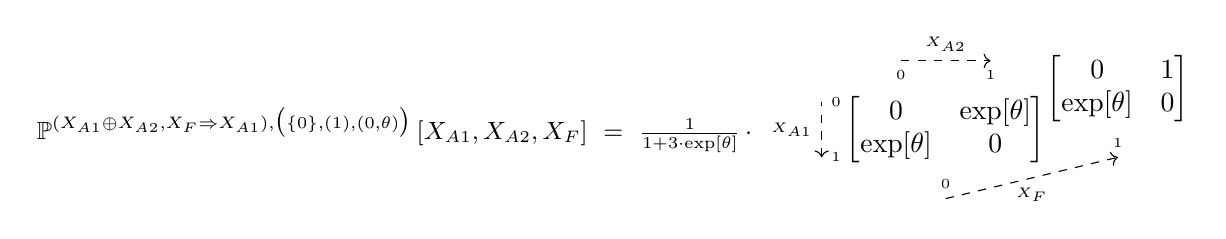
\begin{tikzpicture}[scale=1.75]
            \node (A) at (-4,0) {\corelabelsize $\probofat{(\catvariableof{A1}\oplus\catvariableof{A2},\catvariableof{F}\Rightarrow\catvariableof{A1}),\big(\{0\},(1),(0,\theta)\big)}{\catvariableof{A1},\catvariableof{A2},\catvariableof{F}} \,\, = \,\, \frac{1}{1+3 \cdot \expof{\canparam}} \, \cdot $};
            \node (A) at (0,0) {
                $\begin{bmatrix}
                     0 & \exp[\canparam] \\
                     \exp[\canparam] & 0
                \end{bmatrix}$
            };
            \node (A) at (1.25,0.3) {
                $\begin{bmatrix}
                     0 & 1 \\
                     \exp[\canparam] & 0
                \end{bmatrix}$
            };
            \draw[->,dashed] (-0.325,0.5) node[below] {\tiny $0$} -- (0.325,0.5) node [midway, above] {\tiny $\catvariableof{A2}$} node[below] {\tiny $1$};
            \draw[<-,dashed] (-0.9,-0.2) node[right] {\tiny $1$} -- (-0.9,0.2) node [midway, left] {\tiny $\catvariableof{A1}$} node[right] {\tiny $0$};
            \draw[->,dashed] (0,-0.5) node[above] {\tiny $0$} -- (1.25,-0.2) node [midway, below] {\tiny $X_F$} node[above] {\tiny $1$};
        \end{tikzpicture}
    \end{center}
\end{example}


\subsection{Parameter estimation in \HybridLogicNetworks{}}\label{sec:paramEst}

%% Likelihood maximization
Let us now briefly discuss how \HybridLogicNetworks{} can be trained on data based on likelihood maximization.
Given a dataset $\dataset$ consisting of $\datanum$ independent and identically distributed samples from an unknown distribution, we want to find a \HybridLogicNetwork{} $\hlnwith$ with a statistic $\sstat=(\formulaof{0},\dots,\formulaof{\seldim-1})$ that minimizes the negative log likelihood
\begin{align*}
    \lossof{\hybridparam} \coloneqq -\frac{1}{\datanum} \sum_{\datindexin} \lnof{\probofat{\hlnparameters}{\shortcatvariables=\shortcatindices^{\datindex}}}
    \, .
\end{align*}
% We notice that this is $\infty$ if and only if there is a data point $\datindexin$ with
% \begin{align*}
%     \hlnformulaat{\shortcatvariables=\shortcatindices^{\datindex}}=0 \, ,
% \end{align*}    
% \janina{where the tuple $(A,y_A)$ denotes the hard logic part of the network, $t=(f_1,\dots,f_L)$, and
% \begin{align*}
%     \hlnformulawith =
%     \left(\bigwedge_{\selindex\in\hardlegset\wcols\headindexof{\selindex}=1} \enumformulaat{\shortcatvariables}\right)
%     \land
%     \left(\bigwedge_{\selindex\in\hardlegset\wcols\headindexof{\selindex}=0} \lnot\enumformulaat{\shortcatvariables}\right).
% \end{align*} (Moved from theorem in next subsection to here.)}
% If this is not the case, w
We can rewrite the loss using the empirical mean vector $\datameanwith\in\parspace$, which is defined for $\selindexin$ as
\begin{align*}
    \datameanat{\indexedselvariable}
    = \frac{1}{\datanum} \sum_{\datindexin} \formulaofat{\selindex}{\shortcatvariables=\shortcatindices^{\datindex}} \, ,
\end{align*}
by
\begin{align*}
    \lossof{\hybridparam} =
    \contraction{\datameanwith,\canparamwith} - \lnof{\contraction{\paracttensorwith,\bencsstatwith}} \, .
\end{align*}
Since $\hardparam$ influences only the second term, the best hard parameters can be found by
\begin{align*}
    \hardlegset = \{\selindex \wcols \datameanat{\indexedselvariable}\in\ozset\} \andspace
    \headindexof{\selindex} = \datameanat{\indexedselvariable} \quad \text{for} \quad \selindex\in\variableset \, .
\end{align*}
We further optimize the coordinates $\selindex\in[\seldim]\setexcept{\hardlegset}$ of $\canparamwithin$ alternately by the coordinate descent steps
\begin{align*}
    \difofwrt{\lossof{\hybridparam}}{\canparamat{\indexedselvariable}} = 0
    \Leftrightarrow
    \canparamat{\indexedselvariable}
    = \lnof{
        \frac{\meanparamat{\indexedselvariable}}{(1-\meanparamat{\indexedselvariable})}
        \cdot \frac{\hypercoreat{\headvariableof{\selindex}=0}}{\hypercoreat{\headvariableof{\selindex}=1}}
    } \, .
\end{align*}
where
\begin{align*}
    \hypercoreat{\headvariableof{\selindex}}
    = \contractionof{\{\bencodingof{\formulaof{\secselindex}} \wcols \secselindex\in[\seldim]\}
        \cup\{\softactsymbolof{\secselindex,\canparam} \wcols \secselindex\in[\seldim]\ncond\secselindex\neq\selindex\}
        \cup\{\basemeasure\}}{\headvariableof{\selindex}} \, .
\end{align*}
Based on an interpretation of the coordinate descent steps as matching steps for the mean parameters or moments to $\formulaof{\selindex}$, we call this method \emph{alternating moment matching} for \HybridLogicNetworks{} and provide pseudocode for it it in \algoref{alg:AMM_HLN}.
%% Forward inference in inner loop
We notice that, during the coordinate descent steps, computing the marginal probability of the variable $\headvariableof{\selindex}$ with respect to the current network parameters is required.
This is the computational bottleneck of the algorithm and can be approached by various approximate inference methods, e.g., variational inference (see for example the CAMEL method \cite{ganapathi_constrained_2008}).

\begin{algorithm}[hbt!]
    \caption{Alternating Moment Matching for \HybridLogicNetworks{}}\label{alg:AMM_HLN}
    \begin{algorithmic}
        \Require Mean parameter $\datameanwith$
        \Ensure Parameters $\hybridparam$ for the approximating HLN $\expdist$ %, such that $\expdist$ is the (approximative) moment projection of $\empdistribution$ onto $\hlnsetof{\formulaset}$
        \iosepline
        \State Set
        \begin{align*}
            \hardlegset = \Big\{ \selindex \wcols \selindexin \ncond \meanparamat{\indexedselvariable}\in\{0,1\} \Big\}
        \end{align*}
        and a tuple $\headindexof{\hardlegset}$ with $\headindexof{\selindex}=\meanparamat{\indexedselvariable}$ for $\selindex\in\hardlegset$.
        \State Set $\canparamwith=\zerosat{\selvariable}$
        \While{Convergence criterion is not met}
            \ForAll{$\selindex\in[\seldim]\setexcept{\hardlegset}$}
                \State Compute
                \begin{align*}
                    \hypercoreat{\headvariableof{\selindex}}
                    = \contractionof{\{\bencodingof{\formulaof{\secselindex}} \wcols \secselindex\in[\seldim]\}
                        \cup\{\softactsymbolof{\secselindex,\canparam} \wcols \secselindex\in[\seldim]\ncond\secselindex\neq\selindex\}
                        \cup\{\basemeasure\}}{\headvariableof{\selindex}}
                \end{align*}
                \State Set
                \begin{align*}
                    \canparamat{\indexedselvariable} = \lnof{
                        \frac{\meanparamat{\indexedselvariable}}{(1-\meanparamat{\indexedselvariable})}
                        \cdot \frac{\hypercoreat{\headvariableof{\selindex}=0}}{\hypercoreat{\headvariableof{\selindex}=1}}
                    }
                \end{align*}
            \EndFor
        \EndWhile
        \State \Return $(\hardlegset,\headindexof{\hardlegset},\canparamwith)$
    \end{algorithmic}
\end{algorithm}

It can be shown that the algorithm converges if and only if there is a \HybridLogicNetwork{} matching the empirical moments of the data.
For more details we refer to~\cite[Chapter~9]{goessmann_tensor-network_2025}.

\begin{example}[Continuation of \exaref{exa:hlnAccountingRep}]
    Let us recall the statistic of \exaref{exa:hlnAccountingRep} and consider a dataset of $\datanum=20$ states summarized in the frequency table:
    \begin{center}
        \begin{tabular}{|c|ccc|}
            \hline
            \textbf{Frequency in Dataset} & $\catindexof{A1}$ & $\catindexof{A2}$ & $\catindexof{F}$ \\
            \hline
            0                             & 0                    & 0                    & 0                   \\
            0                             & 0                    & 0                    & 1                   \\
            7                             & 0                    & 1                    & 0                   \\
            2                             & 0                    & 1                    & 1                   \\
            1                             & 1                    & 0                    & 0                   \\
            10                            & 1                    & 0                    & 1                   \\
            0                             & 1                    & 1                    & 0                   \\
            0                             & 1                    & 1                    & 1                   \\
            \hline
        \end{tabular}
    \end{center}
    We then have for the satisfaction rates of $\formulaof{0}=\catvariableof{A1}\oplus\catvariableof{A2}$ and $\formulaof{1}=\catvariableof{F}\Rightarrow\catvariableof{A1}$
    \begin{align*}
        \datameanat{\selvariable=0} = \frac{20}{20} = 1 \andspace
        \datameanat{\selvariable=1} = \frac{7+1+10}{20} = 0.9 \, .
    \end{align*}
    Then \algoref{alg:AMM_HLN} yields with a reasonable convergence criterion choice (such as finite iterations or convergence of $\canparamat{\selvariable}$)
    \begin{align*}
        \hardlegset = \{0\} \quad, \quad \headindexof{\hardlegset} = 1 \andspace
        \canparamat{\selvariable} =
        \begin{bmatrix}
            0 \\
            \lnof{(\frac{0.9}{0.1})\cdot(\frac{1}{3})}
        \end{bmatrix}
        =
        \begin{bmatrix}
            0 \\
            \lnof{3}
        \end{bmatrix}
        \approx
        \begin{bmatrix}
            0 \\
            1.098612
        \end{bmatrix} \, .
    \end{align*}
    To derive this, we notice that \algoref{alg:AMM_HLN} treats formula $\formulaof{0}$ as a hard constraint and assigns $\hardlegset = \{0\}$ and $\headindexof{\hardlegset} = 1$.
    In the $\mathrm{While}$ loop we then have for the formula $\formulaof{1}$
    \begin{align*}
        \hypercoreat{\headvariableof{1}}
        = \contractionof{\bencodingofat{\formulaof{0}}{\headvariableof{0},\catvariableof{F},\catvariableof{A1},\catvariableof{A2}},
            \bencodingofat{\formulaof{1}}{\headvariableof{1},\catvariableof{F},\catvariableof{A1},\catvariableof{A2}}}{\headvariableof{1}}
        = \begin{bmatrix}
              1 \\
              3
        \end{bmatrix}
    \end{align*}
    since $\formulaof{0}$ has $4$ models, of which $3$ are also models of $\formulaof{1}$ and $1$ is instead a model of $\lnot\formulaof{1}$.
    Notice, that the tensor $\hypercoreat{\headvariableof{1}}$ will not change in any further iteration of the $\mathrm{While}$ and the parameter $\canparamat{\selvariable=1}$ will therefore stay constant until the termination of the algorithm.
%    We compare these with the satisfaction rates of $\formulaof{1}$
\end{example}


\subsection{Entailment by \HybridLogicNetworks{}} % Now

Let us now demonstrate a further use of our unified treatment of probabilistic and logical models by investigating a generalized concept of entailment.
Entailment can be generalized to probabilistic models by deciding whether a propositional formula is always satisfied given a probabilistic model.

\begin{theorem}\label{the:hybridEntailment}
    Let $\probofat{\hlnparameters}{\shortcatvariables}$ be a \HybridLogicNetwork{} and $\secexformulaat{\shortcatvariables}$ a propositional formula.
    Then $\probof{\hlnparameters}$ probabilistically entails $\secexformula$, that is,
    \begin{align*}
        \contraction{\probofat{\hlnparameters}{\shortcatvariables},\secexformulaat{\shortcatvariables}} = 1 \, ,
    \end{align*}
    if and only if
    \begin{align*}
        \hlnformula \models \secexformula \, ,
    \end{align*}
    where
    \begin{align*}
        \hlnformulawith =
        \left(\bigwedge_{\selindex\in\hardlegset\wcols\headindexof{\selindex}=1} \enumformulaat{\shortcatvariables}\right)
        \land
        \left(\bigwedge_{\selindex\in\hardlegset\wcols\headindexof{\selindex}=0} \lnot\enumformulaat{\shortcatvariables}\right).
    \end{align*} 
\end{theorem}
\begin{proof}
    We have
    \begin{align*}
        \contraction{\probofat{\hlnparameters}{\shortcatvariables},\secexformulaat{\shortcatvariables}} = 1
    \end{align*}
    if and only if 
    \begin{align*}
        \contraction{\probofat{\hlnparameters}{\shortcatvariables},\secexformulaat{\shortcatvariables}-\onesat{\shortcatvariables}} = 0
    \end{align*}
    which is equal to 
    \begin{align*}
        \contraction{\probofat{\hlnparameters}{\shortcatvariables},\lnot\secexformulaat{\shortcatvariables}} = 0 \, .
    \end{align*}
    Since $\probofat{\hlnparameters}{\shortcatvariables}$ is non-negative this is equivalent to
    \begin{align*}
        \contraction{\nonzeroof{\probofat{\hlnparameters}{\shortcatvariables}},\lnot\secexformulaat{\shortcatvariables}} = 0 \, .
    \end{align*}
    We use that
    \begin{align*}
        \nonzeroof{\probofat{\hlnparameters}{\shortcatvariables}} 
        = \hlnformulawith 
    \end{align*}
    and get that this is further equivalent to
    \begin{align*}
        \contraction{\hlnformulawith ,\lnot\secexformulaat{\shortcatvariables}} = 0 \, ,
    \end{align*}
    which is by \defref{def:logicalEntailment} $\hlnformula \models \secexformula$.
\end{proof}

\begin{example}[Continuation of \exaref{exa:hlnAccountingAMM}]
    Let us consider again the \HybridLogicNetwork{} $\probof{(\catvariableof{A1}\oplus\catvariableof{A2},\catvariableof{F}\Rightarrow\catvariableof{A1}),\big(\{0\},(1),(0,\lnof{3})\big)}$ from \exaref{exa:hlnAccountingAMM} and assume we want to decide the probabilistic entailment of the formula
    \begin{align*}
        \secexformulaat{\catvariableof{A1},\catvariableof{A2},\catvariableof{F}}
        = \lnot\catvariableof{A1} \lor \lnot\catvariableof{A2} \lor \lnot\catvariableof{F} \, ,
    \end{align*}
    which has all states but $(1,1,1)$ as a model (and is therefore refered to as a maxterm).
    Using \theref{the:hybridEntailment} we have that
    \begin{align*}
        \contraction{\probofat{(\catvariableof{A1}\oplus\catvariableof{A2},\catvariableof{F}\Rightarrow\catvariableof{A1}),\big(\{0\},(1),(0,\lnof{3})\big)}{\catvariableof{A1},\catvariableof{A2},\catvariableof{F}},\secexformulaat{\catvariableof{A1},\catvariableof{A2},\catvariableof{F}}} =1
    \end{align*}
    if and only if $\catvariableof{A1}\oplus \catvariableof{A2} \models \lnot\catvariableof{A1} \lor \lnot\catvariableof{A2} \lor \lnot\catvariableof{F}$.
    By \defref{def:logicalEntailment} this entailment holds, since by the De-Morgan rule
    \begin{align*}
        \contraction{\catvariableof{A1}\oplus \catvariableof{A2},\lnot \left(\lnot\catvariableof{A1} \lor \lnot\catvariableof{A2} \lor \lnot\catvariableof{F}\right)}
        &= \contraction{\catvariableof{A1}\oplus \catvariableof{A2},\catvariableof{A1},\catvariableof{A2},\catvariableof{F}} \\
        &= \contraction{\catvariableof{F}} \cdot \contraction{\catvariableof{A1}\oplus \catvariableof{A2},\catvariableof{A1},\catvariableof{A2}} \\
        &= 0 \, .
    \end{align*}
    We thus conclude, that $\secexformula$ is probabilistically entailed by $\probof{(\catvariableof{A1}\oplus\catvariableof{A2},\catvariableof{F}\Rightarrow \catvariableof{A1}),\big(\{0\},(1),(0,\lnof{3})\big)}$.
\end{example}
%\section{Implementation}\label{sec:code}

\alex{Needs a major overwork: Present tnreason architecture, capabilities, add examples from reasoning.}

The architecture can be conveniently implemented with the python package \tnreason{}. 
Multiple examples including graph-coloring, sat problems, Sudoku, and temporal clue are available\footnote{\url{https://github.com/EnexaProject/enexa-tensor-reasoning/tree/version1}}.
To emphasize the intuitive implementation of CANs, a code snippet for the implementation of a CAN for the sat problem $f[X_a=a,X_b=b,X_c=c]=(a \lor b) \land \lnot c$ described in example~\ref{exa:bencodingNegCon} is explained.
This propositional formula is encoded by a dictionary of variables encoded by nested lists, that need to all be fulfilled.
% \begin{minted}{python}
%      clauseList = [{"a": 1, "b": 1}, {"c": 0}]
% \end{minted}
\begin{minted}{python}
expressionsDict = {"f0" :  ["and", ["or", "a", "b"], ["not", "c"]]}
\end{minted}
After importing the package by
\begin{minted}{python}
from tnreason import representation, application, engine
\end{minted}
the CAN can then be build by defining all cores. Activation cores then have suffices \mintinline{python}{_aC} and computation cores are denoted with suffices \mintinline{python}{_cC} by
\begin{minted}{python}
cores = application.create_cores_to_expressionsDict(expressionsDict)
computationCores = {key: value for key, value in cores.items() 
                                                         if key.endswith("_cC")}
\end{minted}
The generated \mintinline{python}{computationCores} is a dictionary with the following keys and tensors of given shapes as expected in example~\ref{exa:bencodingNegCon}.
\begin{minted}{python}
'f0_aC', [2]
'(and_(or_a_b)_(not_c))_cC', [2, 2, 2]
'(or_a_b)_cC', [2, 2, 2]
'(not_c)_cC', [2, 2]
\end{minted}
Based on this dictionary, the \ComputationActivationNetwork{} can be build by setting the activation network for the single output feature (the output of $f$) to a vector acting on the output of the basis encoding of $f$. Here a \mintinline{python}{SingleHybridFeature} is used, which allows for hard or soft activations. Then the value for the desired output of the feature is set to \mintinline{python}{True}.
\begin{minted}{python}
caNet = representation.ComputationActivationNetwork(
    computationCoreDict=computationCores,
    featureDict={"f0" : representation.SingleHybridFeature(
                                    featureColor="(and_(or_a_b)_(not_c))_cV")},
    canParamDict={"f0" : True}
    )
\end{minted}

As in example~\ref{exa:bencodingNegCon}, the CAN then has the following form.\alex{Should we use the engine.draw() for that?}
\begin{center}
\begin{tikzpicture}[scale=0.4, yscale=-1, thick] % , baseline = -3.5pt
        
            \begin{scope}
                [shift={(7,0)}]
        
                \draw[->-] (0,1)--(0,-1) node[midway,left] (Xa) {\colorlabelsize $\catvariableof{a}$};
                \draw[->-] (3,1)--(3,-1) node[midway,right] {\colorlabelsize $\catvariableof{b}$};
                \draw[->-] (6,1)--(6,-1) node[midway,right] {\colorlabelsize $\catvariableof{c}$};
        
                \draw (-2.5,-1) rectangle (4, -3);
                \node[anchor=center] (or) at (0.7,-2) {\corelabelsize \mintinline{python}{'(or_a_b)_cC'}};
        
                \draw[->-] (1.5,-3) --(1.5,-5) node[midway,right]{\colorlabelsize $\headvariableof{a \lor b}$};
        
                \draw (5,-1) rectangle (11, -3);
                \node[anchor=center] (not) at (8,-2) {\corelabelsize\mintinline{python}{'(not_c)_cC'}};
        
                \draw[->-] (6,-3) --(6,-5) node[midway,right]{\colorlabelsize $\headvariableof{\lnot c}$};
        
                \draw (-2.9,-5) rectangle (10,-7);
                \node[anchor=center] (and) at (3.5,-6) {\corelabelsize \mintinline{python}{'(and_(or_a_b)_(not_c))_cC'}};
        
                \draw[->-] (4,-7) -- (4,-8.5) node[right] (Yand) {\colorlabelsize $\headvariableof{(a \lor b) \land \lnot c}$};
                \drawvariabledot{4}{-8}
                \draw[] (4,-8) -- (4,-9);
                \draw (3,-9) rectangle (5,-11);
                \node[anchor=center] (f0) at (4,-10) {\mintinline{python}{"f0"}};

                  \node[
                    draw=teal,
                    line width=1.2pt,
                    ellipse,
                    fit=(or)(not)(and)(Xa),
                    inner xsep=8mm,   % horizontal padding
                    inner ysep=0mm     % vertical padding
                  ] (tealring) {};
                  \node[teal] at (20,0) {computation network};

                  
                  \node[
                    draw=purple!50,
                    line width=1.2pt,
                    ellipse,
                    fit=(f0)(Yand),
                    inner xsep=8mm,   % horizontal padding
                    inner ysep=0.2mm     % vertical padding
                  ] (tealring) {};
                  \node[purple!50] at (15.5,-8.5) {activation network};
            \end{scope}
\end{tikzpicture}
\end{center}

The other representation in example~\ref{exa:bencodingNegCon} can also be implemented.
Both architectures can be found the linked notebook\footnote{\url{https://colab.research.google.com/drive/14knFuMJHI683DAmUgJ-G10MQFueoXR6q\#scrollTo=vrOYBViZhX2S}}.
Note that more efficient representations of this network are possible and the one described here is mainly for pedagogic purposes.
Furthermore the right implementation of the formula can be checked by contractions.
\begin{minted}{python}
allCores = caNet.create_cores()
formula = engine.contract(coreDict = allCores, 
                          openColors=["a_dV","b_dV", "c_dV"])
assert formula[{"a_dV": 1, "b_dV" : 1, "c_dV" : 0}] == 1
assert formula[{"a_dV": 1, "b_dV" : 1, "c_dV" : 1}] == 0
\end{minted}
The notebook also shows how the network can be normalized to represent a uniform probability distribution over all models of the formula.
\begin{minted}{python}
distribution = engine.normalize(coreDict = allCores, 
                                outColors = ["a_dV","b_dV", "c_dV"], 
                                inColors = [])
assert distribution[{"a_dV": 1, "b_dV" : 1, "c_dV" : 0}] == 1/3
assert distribution[{"a_dV": 1, "b_dV" : 1, "c_dV" : 1}] == 0
\end{minted}

% \newpage
% \begin{minted}{python}
% def get_clauseList_as_CANetwork(clauseList, evidenceDict=dict()):
%     """
%     Prepares the SAT instance as a Computation-Activation Network
%     """
    
%     # The computation network encodes all individual statistics of interest. 
%     # For SAT, they are individual formulas connected by $\lhat$ (Section 3.4).
%     # Here, they are $\lnot a \lor b$ and $c$. (The names are irrelevant.)
%     compDict = {
%         "clauseCore_" + str(i): create_clause_core(clauseDict) 
%         for i, clauseDict in enumerate(clauseList)
%     }
    
%     # The atomic variables are all $0/1$ variables in the formula. 
%     # Here, they are $a,b,c$.
%     atomVariables = list({key for clause in clauseList for key in clause.keys()})
    
%     # The a feature dictionary collects all variables in the network.
%     # Here, only $0/1$-vectors build by HardPartitionFeature are considered.
%     featDict = {
%         # One entry for each variable interesting for the solution $X_a,X_b,X_c$
%         **{"atomFeature_" + atomKey: 
%             representation.HardPartitionFeature(
%                 featureColors=[atomKey], 
%                 affectedComputationCores={})
%                 for atomKey in atomVariables},
%         # One entry for each "hidden" variable not part of the solution 
%         # $Y_{a\lor b}$ and $Y_c$
%         **{"clauseFeature_" + str(i): 
%             representation.PassiveFeature(
%                 featureColors=list(clauseDict.keys()), 
%                 affectedComputationCores={
%                 "clauseCore_" + str(i)}, shape=[])
%            for i, clauseDict in enumerate(clauseList)},
%     }
%     # The variables, that are already known, are collected in a dictionary. 
%     # In Sudoku, this would be the initial board.
%     ParDict = {evidenceKey: 
%         representation.create_basis_core(
%             name=evidenceKey, shape=[2],
%             colors=[evidenceKey],
%             numberTuple=[evidenceDict[evidenceKey]])
%         for evidenceKey in evidenceDict
%     }
%     return representation.ComputationActivationNetwork(
%         featureDict=featDict,
%         computationCoreDict=compDict,
%         canParamDict=ParDict
%     )
% \end{minted}
% \janina{How is the activation network added?}
% \begin{minted}{python}
% expressionsDict = {„formula1“: [„or“,“a“,“b“], „formula2“: [„not“,“c“]}
% featureDict = {„formula1“: SingleHybridFeature(featureColors=[„(or_a_b)“])}
% canParamDict = {„formula1“ : True}
% \end{minted}



% \begin{minted}{python}
% def generate_CANetwork(graph, colorNum, coreType, allowedColorDict={}):
%     compDict = {
%         nodeColor0 + "_" + nodeColor1: 
%         get_color_constraint_core(
%             nodeColor0, 
%             nodeColor1, 
%             colorNum, 
%             coreType
%             )
%         for nodeColor0, nodeColor1 in graph.edges
%         }
%     featDict = {
%         **{nodeColor:
%             representation.HardPartitionFeature(
%                 featureColors=[nodeColor], 
%                 shape=[colorNum]
%                 )
%             for nodeColor in graph.nodes
%             },
%         **{nodeColor0 + "_" + nodeColor1:
%             representation.PassiveFeature(
%                 featureColors=[],
%                 shape=[],
%                 affectedComputationCores=[nodeColor0 + "_" + nodeColor1]
%                 )
%             for nodeColor0, nodeColor1 in graph.edges
%             }
%         }
%     return representation.ComputationActivationNetwork(
%         computationCoreDict=compDict,
%         featureDict=featDict,
%         canParamDict=allowedColorDict,
%         )
% \end{minted}
\chapter{Implementation in the \tnreason{} package}\label{cha:implementation}

We here document the implementation of the discussed concepts in the \python{} package \tnreason{}, in the version \curvertnreason

% Name
\tnreason{} is an abbreviation of \textbf{t}ensor \textbf{n}etwork \textbf{reason}ing, by which we emphasize the capabilities of this package to represent and answer reasoning tasks by tensor network contractions.

% Installation
The package can be installed either by cloning the repository
\begin{center}
    \href{https://github.com/EnexaProject/enexa-tensor-reasoning}{https://github.com/EnexaProject/enexa-tensor-reasoning}
\end{center}
or by
\begin{lstlisting}
!pip install tnreason==2.0.0
\end{lstlisting}

\sect{Architecture}

\tnreason{} is structured in four subpackages and three layers
\begin{itemize}
    \item Layer 1: Storage and numerical manipulations, by subpackage \spengine{}
    \item Layer 2: Specification of workload, subpackage \sprepresentation{} specific for storage, subpackage \spreasoning{} specific for manipulations
    \item Layer 3: Applications in reasoning, by subpackage \spapplication{}
\end{itemize}

We sketch this structure by
\begin{center}
    %! Author = alexgoessmann
%! Date = 09.03.25

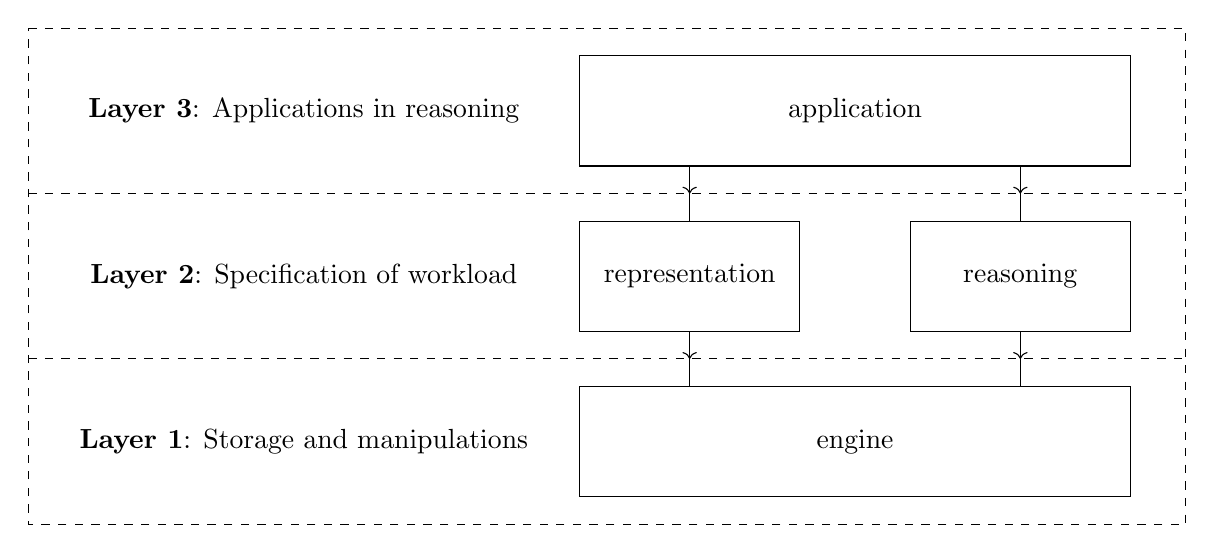
\begin{tikzpicture}[scale=0.35]
    \draw[dashed] (-30,15) -- (12,15) -- (12,-3) -- (-30,-3) -- (-30,15);

    \draw (-10,10) rectangle (10,14);
    \node [anchor=center] at (0,12) {\spapplication{}};

    \node [anchor=center] at (-20,12) {\layerthreespec};
    \draw[dashed] (-30,9) -- (12,9);
    \node [anchor=center] at (-20,6) {\layertwospec};

    \draw[->-] (6,10) -- (6,8);
    \draw (2,4) rectangle (10,8);
    \node [anchor=center] at (6,6) {\spreasoning{}};
    \draw[->-] (6,4) -- (6,2);

    \draw[->-] (-6,10) -- (-6,8);
    \draw (-10,4) rectangle (-2,8);
    \node [anchor=center] at (-6,6) {\sprepresentation{}};
    \draw[->-] (-6,4) -- (-6,2);

    \draw[dashed] (-30,3) -- (12,3);
    \node [anchor=center] at (-20,0) {\layeronespec};

    \draw (-10,-2) rectangle (10,2);
    \node [anchor=center] at (0,0) {\spengine{}};
\end{tikzpicture}
\end{center}


\sect{Implementation of basic notation}

First of all, we explain how the basis notation explained in \charef{cha:notation} is reflected in the implementation.

\subsect{\bncategoricals}
Categorical Variables are identified by strings, which then appear as colors of the corresponding tensor axes.
Their dimension is stored in shapeDicts, but most practically these shapes are stored in the tensors in which variables appear.
Suffixes in the color string (defined in \inlinecode{representation.suffixes}) denote the type of the variable:
\begin{itemize}
    \item Distributed variables with color suffix \disVarSuf: $\catvariableof{\cdot}$
    \item Computed variables with color suffix \comVarSuf: $\headvariableof{\cdot}$
    \item Selection variables with color suffix \selVarSuf: $\selvariableof{\cdot}$
    \item Term variables with color suffix \terVarSuf: $\indvariableof{\cdot}$
\end{itemize}

\subsect{\bntensors}

\paragraph{Tensors} are objects of classes inheriting \inlinecode{engine.TensorCore} with main attributes
\begin{itemize}
    \item \inlinecode{values}: Storing the coordinates of the tensors (individual realization for different cores)
    \item \inlinecode{colors}: List of the variables $[\headvariableof{\formula},\catvariableof{0},\catvariableof{1}]$
    \item \inlinecode{name}: Reflecting the notation such as $\bencodingof{\formula}$
    \item \inlinecode{shape}: Storing the dimension of each appearing variable, as a list of integers with the same length as colors.
\end{itemize}

Suffixes in the name string (defined in \inlinecode{representation.suffixes}) highlight the origin and purpose of the tensor.
Cores are named with suffixes based on their functionality
\begin{itemize}
    \item Computation core with name suffix \comCoreSuf: They represent the computation of a function in basis calculus, and are directed cores.
    Their colors are \inlinecode{[headColors] + [inputColors]}, where \inlinecode{[inputColors]} are either distributed variables or, if having a composition of formulas.
    When the function is a selection augmentation of other functions, selection colors are listed in the end of \inlinecode{[inputColors]}.
    \item Activation core with name suffix \actCoreSuf: two-dimensional vectors representing of the activation core to a formula
\end{itemize}

Both the cores and the colors are further refined by infixes before the suffices to denote specific instantiations.

\begin{itemize}
    \item \selCoreIn: Involving a selection variable
    \item \eviCoreIn: Storing evidence about a variable
    \item \heaIn: Head of a function, typically the variable computed at a activation selector
    \item \funIn: Function selection variables
    \item \posIn+\stringof{i}: Variable selection for argument at position $i$
    \item \datIn: Involving data (data cores and colors)
\end{itemize}

Further infixes are strings denoting atom names and neuron names.

Exploiting efficient representation tricks we further have the tensor name suffices:
\begin{itemize}
    \item \atoCoreSuf: Atomization core, for sparse representation of categorical constraints
    \item \vselCoreSuf: Variable selection core: For sparse representation of variable selectors
\end{itemize}

\paragraph{Initialization}
Tensors are instantiated by
\begin{lstlisting}
engine.getCore(coreType)(values, colors, name, shape)
\end{lstlisting}
where \inlinecode{coreType} is a string further specifying a specific implementation of tensors (see for more detail \secref{sec:implementationEngine}).
The default tensor implementation \defaultCoreType is chosen, when \inlinecode{coreType} is not specified.


One-hot encodings are specific tensors created in \sprepresentation{}.

\subsect{\bncontractions}

\paragraph{Tensor networks} $\tnetof{\graph}=\{\hypercoreofat{\edge}{\catvariableof{\edge}}\wcols\edge\in\edges\}$ are stored as dictionaries of tensors, where the keys coincide with the names of the corresponding tensors.
The edges of the hypergraph $\graph$ used in the definition of tensor networks in \defref{def:tensorNetwork} are here labeled by the names of the tensors and the affected variables by the list of colors, being an attribute of each tensor.

\paragraph{Contractions} are implemented in the subpackage \spengine{}, orienting on \defref{def:contraction}.
Reflected in the notation
\begin{align*}
    \contractionof{\tnetof{\graph}}{\secnodevariables}
\end{align*}
a contraction is defined by
\begin{itemize}
    \item Tensor Network $\tnetof{\graph}$, specified by a dictionary of tensor names as keys and valued by tensor cores.
    \item Open Variables $\secnodes$, specified by a list of colors to the variables.
\end{itemize}
Contraction calls are implemented as
\begin{lstlisting}
engine.contract(contractionMethod, coreDict, openColors, dimensionDict, evidenceColorDict)
\end{lstlisting}
where the arguments are
\begin{itemize}
    \item \inlinecode{contractionMethod}: str, chooses one of the contraction providers. The default contraction method \defaultContractionMethod is chosen, when
    \item \inlinecode{coreDict}: Dictionary of TensorCores (of the above formats), representing the Tensor Network $\tnetof{\graph}$
    \item \inlinecode{openColors}: List of str, each str identifying a color, that is a variable to be left open in the contraction
    \item \inlinecode{dimensionDict}: Dict valued by int and keys by str, storing dimensions to each variable. This is of optional usage, when a color in openColors does not appear in the coreDict.
    \item \inlinecode{evidenceColorDict}: Dict valued by int and keys by str, indicating sliced variables
\end{itemize}

Coordinates of tensors can be retrieved by
\begin{align*}
    \contractionof{\hypercoreat{\nodevariables}}{\secnodevariables=\catindexof{\secnodes}} \, .
\end{align*}
We implement this by leaving \inlinecode{openColors} empty and passing $\catindexof{\secnodes}$ as the \inlinecode{evidenceColorDict}, as a dictionary with keys by the \inlinecode{str} colors to the variables and values by the corresponding \inlinecode{int} indices.

Graphical illustrations can be generated by
\begin{lstlisting}
engine.draw_factor_graph(coreDict)
\end{lstlisting}
where \inlinecode{coreDict} is a tensor network to be visualized.


\subsect{\bnencoding}
Encoding schemes are implemented in the subpackage \sprepresentation{}.



\sect{Subpackage \spengine{}}\label{sec:implementationEngine}

The \spengine{} subpackage is for the storage and numerical manipulation of tensors and tensor networks.
We organize the subpackage as the lowest layer of \tnreason{}, specializing in storage of Tensor Networks and performing the contractions.

\subsect{Basis+ $\cpformat$ Decompositions storing \inlinecode{values}}

\paragraph{Specification of basis+ elementary tensors}
We orient on basis+ sparse tensor decomposition in the initialization of tensor cores, as discussed in detail in \charef{cha:sparseRepresentation}.
The basis+ elementary tensors have basis+ $\cpformat$ rank of $1$ and admit a decomposition as (see \defref{def:polynomialSparsity})
\begin{align*}
    \hypercoreat{\nodevariables}
    = \slicescalar \cdot \contractionof{\onehotmapofat{\catindexof{\variableset}}{\catvariableof{\variableset}}}{\nodevariables} \, .
\end{align*}
Elementary basis+ tensors are in \tnreason{} stored by a tuple
\begin{lstlisting}
(value, posDict)
\end{lstlisting}
where \inlinecode{posDict} specifies the values to the variables, which do not have a trivial leg vector, and \inlinecode{value} a scalar scaling the basis vector.
Comparing with the notation of \charef{cha:sparseRepresentation}, the keys of \inlinecode{posDict} correspond with $\variableset$, the values of \inlinecode{posDict} with $\catindexof{\variableset}$ and \inlinecode{value} corresponds with $\slicescalar$.

\paragraph{Elementary Iterators}
The initialization, coordinate retrieval and conversion operations of all tensor cores are oriented on basis+ $\cpformat$ Decompositions \eqref{eq:decIntoMonomials} of tensors.
A tensor
\begin{align*}
    \hypercoreat{\nodevariables}
    = \sum_{\slicetupleof{}\in\sliceset} \slicescalar \cdot \contractionof{\onehotmapofat{\catindexof{\variableset}}{\catvariableof{\variableset}}}{\nodevariables} \, .
\end{align*}
corresponds with an iterator over tuples \inlinecode{(value,posDict)}, each specifying a basis+ elementary tensor in the sum.
%Each tensor core can be iterated, where the iterations are over tuples \inlinecode{(value,posDict)} specifying a basis+ tensor.

\paragraph{Core Arithmetics}
When subscribing an instance \inlinecode{exampleCore} of \inlinecode{engine.TensorCore} by
\begin{lstlisting}
exampleCore[posDict] = value
\end{lstlisting}
a basis+ elementary tensor specified by \inlinecode{(value,posDict)} is added to its values, that is
\begin{align*}
    \hypercoreat{\shortcatvariables} \algdefsymbol \hypercoreat{\shortcatvariables} + \contractionof{\onehotmapofat{\catindexof{\variableset}}{\catvariableof{\variableset}}}{\shortcatvariables} \, .
\end{align*}
The linear structure of tensors spaces are more further reflected in sums of \inlinecode{engine.TensorCore} instances, which are implemented with the same \inlinecode{coreType}, as
\begin{lstlisting}
summed = exampleCore1 + exampleCore2
\end{lstlisting}
and scalar multiplication, where a scalar \inlinecode{value} of type \inlinecode{int} or \inlinecode{float}
\begin{lstlisting}
multiplied = value * exampleCore
\end{lstlisting}
Both operations are performed as manipulations of the tensors \inlinecode{values}.
Contraction of two \inlinecode{engine.TensorCore} instances are performed by
\begin{lstlisting}
contracted = exampleCore1.contract_with(exampleCore2)
\end{lstlisting}
and are used in corewise contraction, where \inlinecode{contractionMethod="CorewiseContractor"}.

\paragraph{Initialization}
Any instance of \inlinecode{engine.TensorCore} is initialized as a vanishing tensor $\onesat{\nodevariables}$, when \inlinecode{values} is not specified.
The values are then assigned by iteration over a \inlinecode{sliceIterator} over \inlinecode{(value,posDict)} tuples specifying elementary basis+ tensors, where the $\cpformat$ rank is the length of the iterator
%A basis+ $\cpformat$ tensor is specified by an iterator \inlinecode{sliceIterator} over elementary basis+ tensors, where the $\cpformat$ rank is the length of the iterator
This initialization is by applied in the method
\begin{lstlisting}
engine.create_from_slice_iterator(shape, colors, sliceIterator, coreType, name)
\end{lstlisting}
where \inlinecode{shape, colors, coreType, name} are used in the call of an empty core by \\
\inlinecode{engine.get_core} and \inlinecode{sliceIterator} used to iterative add the basis+ elementary tensors to create the tensor.

\paragraph{Storage of basis+ $\cpformat$ decompositions}
The implemented tensor classes derived from \\
\inlinecode{engine.TensorCore} differ in their implementation of \inlinecode{values}.
Motivated from basis+ $\cpformat$ decompositions, most classes rely on a data base storing the \inlinecode{(value,posDict)} tuples.
An overview over the derived classes is provided in \figref{tab:tensorClasses}.
Here \inlinecode{PandasCore}, \inlinecode{TentrisCore} and \inlinecode{PolynomialCore} support sparse basis+ $\cpformat$ decompositions, by utilizing \inlinecode{pandas.DataFrame}, \inlinecode{tentris.hypertrie} and \inlinecode{list} as storage data base.
These are implementations of the matrix representation of \remref{rem:matStorageBasPlus}.
The \inlinecode{NumpyCore} class on the other hand is based relies on arrays as \inlinecode{numpy.array} as storage solution, which corresponds with the demand that each \inlinecode{posDict} contains all colors of the tensor.
Effectively, this amounts to restricting to basis $\cpformat$ decomposition, which demanded ranks are always larger than basis+ $\cpformat$ decompositions (see \theref{the:rankCascade}).

\begin{figure}
    \begin{center}
        \begin{tabular}{|c|c|c|c|}
            \hline
            \textbf{coreType}           & \textbf{Used Package}                       & \text{Storage of \inlinecode{values}}             & \textbf{Sparse basis+ $\cpformat$ support} \\
            \hline
            \inlinecode{NumpyCore}      & \inlinecode{numpy}                          & \inlinecode{numpy.array}                          & No                                         \\
            \hline
            \inlinecode{PandasCore}     & \inlinecode{pandas}                         & \inlinecode{pandas.DataFrame}                     & Yes                                        \\
            \hline
            \inlinecode{TentrisCore}    & \inlinecode{tentris}  \cite{bigerl_tentris_2020} & \inlinecode{tentris.hypertrie} & Yes\\
            \hline
            \inlinecode{PolynomialCore} & $--$                                        & \inlinecode{list} of \inlinecode{(value,posDict)} & Yes\\
            \hline
        \end{tabular}
    \end{center}
    \caption{Derived classes from \inlinecode{engine.TensorCore}, differing in the implemented storage of \inlinecode{values}.}\label{tab:tensorClasses}
\end{figure}




\subsect{Contractions}

%\textbf{Binary CP Decomposition}
%
%Based on the monomial decomposition $\polsparsityof{\cdot}$ as specified in \defref{def:polynomialSparsity}.
%To store the values of a tensor we store the slices of tensors by the indices $\catindexof{\variableset}$.
%
%% Trick -> To BinaryCP
%Contractions can be performed by partially contracting the cores of the decomposition.
%In this way, one can avoids coordinatewise storages of high-order tensors, which can be intractable.


% Contraction Method List
The supported contraction methods are listed in \figref{tab:contractionMethods}.

\begin{figure}
    \begin{center}
        \begin{tabular}{|p{\threecolumnwidth}|p{\threecolumnwidth}|p{\threecolumnwidth}|}
            \hline
            \textbf{contractionMethod} (str)   & \textbf{Package}                            & \textbf{Applied procedure}                                \\
            \hline
            \stringof{NumpyEinsum}             & \inlinecode{numpy}                          & Einstein summation \inlinecode{numpy.einsum}              \\
%        \hline
%        \stringof{TensorFlowEinsum}        & $\mathrm{tensorflow}$ & Einstein summation of $\mathrm{tensorflow}$ tensors         \\
%        \hline
%        \stringof{TorchEinsum}             & $\mathrm{torch}$      & Einstein summation of $\mathrm{torch}$ tensors              \\
            %\hline
            \stringof{TentrisEinsum}           & \inlinecode{tentris}  \cite{bigerl_tentris_2020} & Einstein summation \inlinecode{tentris.einsum}            \\
            %\hline
            \stringof{PgmpyVariableEliminator} & \inlinecode{pgmpy}                          & Variable Elimination of \inlinecode{pgmpy.DiscreteFactor} \\
            %\hline
            \stringof{CorewiseContractor}      & $--$                                        & Contraction using \inlinecode{core.contract_with()}       \\
            \hline
        \end{tabular}
    \end{center}
    \caption{Implemented contraction methods in \tnreason{}.}
    \label{tab:contractionMethods}
\end{figure}

\paragraph{Einstein Summation}
is a syntax of specifying the contractions of arrays.
Different possibilities are available to optimize over possible contraction paths, for example in \inlinecode{numpy} by the \inlinecode{numpy.einsum_path}.
%Contractions represented as Einstein summation, as implemented in:
%\begin{itemize}
%	\item numpy
%	\item tensorflow
%	\item pytorch
%	\item tentris
%\end{itemize}

\paragraph{Variable Elimination}
contracts along a junction tree, build by variable elimination.
We here use an implementation in the \inlinecode{pgmpy} package.

\paragraph{Corewise Contraction}
uses the \inlinecode{contract_with} method of tensor cores to contract in a given order.





\sect{Subpackage \sprepresentation{}}\label{sec:implementationRepresentation}

The \sprepresentation{} subpackage consists in a collection of core creation methods.
%Here the basis encodings $\bencodingof{\exfunction}$ of various maps $\exfunction$ are created.
We arrange the \sprepresentation{} subpackage into the second layer of the \tnreason{} architecture, since it specifies tensor cores which formats are specified in \spengine{}.

\paragraph{Coordinate Calculus}
Coordinatewise transformations (see \defref{def:coordinatewiseTransform}) are supported by
\begin{lstlisting}
engine.coordinatewise_transform(coresList, transformFunction)
\end{lstlisting}
where \inlinecode{coresList} is a list of $\seldim$ tensors with identical variables and \inlinecode{transformFunction} a function $\chainingfunction: \parspace \rightarrow \rr$.

\paragraph{Basis Calculus}
Basis encodings (see \defref{def:functionRelationEncoding}) of functions $\exfunction:\facstates \rightarrow \secfacstates$ are created by
\begin{lstlisting}
engine.create_relational_encoding_from_lambda(inshape, outshape, incolors, outcolors, indicesToIndices)
\end{lstlisting}
where \inlinecode{indicesToIndices} is a lambda-function representing $\exfunction$ and \inlinecode{inshape, outshape, incolors, outcolors} specify the input and output variables.
Let us notice, that this procedure produces sums of $\facdim$ basis tensors corresponding with a basis $\cpformat$ decompositions.
More involved initialization procedures based on basis+ elementary tensors calling \\
\inlinecode{engine.create_from_iterator} might result in sparser representations.

\paragraph{Propositional Connectives} are represented by strings.
\figref{tab:connectives} lists the supported logical connectives, which are implemented in \inlinecode{representation.basisplus_calculus}.
If the \inlinecode{str} to the connective starts with \stringof{n}, then the negated connective is encoded.

\begin{figure}
    \begin{center}
        \begin{tabular}{|p{\fivecolumnwidth}|p{\fivecolumnwidth}|p{\threecolumnwidth}|p{\fivecolumnwidth}|p{\fivecolumnwidth}|}
            \hline
            \textbf{$\exconnective$}          & \textbf{$\synencodingof{\exconnective}$} & \textbf{Notes} & $\baspluscprankof{\exconnective}$ & $\baspluscprankof{\bencodingof{\exconnective}}$ \\
            \hline
            $\land$                           & \stringof{and}                           &                                                                   & 1                                 & 3                                               \\
            %\hline
            $\lor$                            & \stringof{or}                            &                                                                   & 2                                 & 3                                               \\
            %\hline
            $\Rightarrow$                     & \stringof{imp}                           & last variable as head, others premises                            & 2                                 & 3                                               \\
            %\hline
            $\oplus$                          & \stringof{xor}                           & implemented as the negation of \stringof{eq}, i.e. \stringof{neq} & 3 & 5 \\
            %\hline
            $\Leftrightarrow$                 & \stringof{eq}                            &                                                                   & 2                                 & 5                                               \\
            %\hline
            $\catvariableof{\atomenumerator}$ & \stringof{pas} + "$\atomenumerator$"     & $\atomenumerator$th atom & 1 & 2 \\
            %\hline
            $\lnot$                           & \stringof{not}                           & negation of the first argument, i.e. \stringof{npas0}             & 1                                 & 2                                               \\
            \hline
        \end{tabular}
    \end{center}
    \caption{Supported connectives in the script language.
    The arity of all connectives is not restricted.
    We notice that the basis+ rank $\baspluscprankof{\bencodingof{\exconnective}}$ is independent of the arity and in most cases less than the naive bound of $2^{\catorder}$.
    }\label{tab:connectives}
\end{figure}


% WOLFRAM Numbers

\paragraph{Wolfram codes} provide a classification scheme of propositional formuals by natural numbers, which is supported in the script language.
%They provide a generic representation scheme of propositional formulas by the so-called
The Wolfram code has been designed for the classification of cellular automaton rules \cite{wolfram_statistical_1983} and popularized in the book \cite{wolfram_new_2002}.
Along this, the coordinate encodings of $\catorder$-ary connectives $\exconnective$ are flattened and interpreted as a binary number, which is transformed into a decimal number and represented as a string $\synencodingof{\exconnective}$.
To be more precise, to each $\catorder$-ary connective its Wolfram code is calculated by
\begin{align*}
    N(\exconnective) = \sum_{\catindex\in[2^\catorder]} 2^{2^{\catorder}-\catindex-1} \cdot \exconnective(\catindex) \, .
\end{align*}
In the script language, the connective is represented by the string concatenation of the arity and the Wolfram code as
\begin{align*}
    \synencodingof{\exconnective} = "\catorder" + "_" + "N(\exconnective)" \, .
\end{align*}

\subsect{Computation Activation Networks}

\paragraph{Features} are generation procedures of activation cores given canonical parameters.
They are initialized by
\begin{lstlisting}
ComputedFeature(featureColors, affectedComputationCores, shape, name)
\end{lstlisting}
where
\begin{itemize}
    \item \inlinecode{featureColors} is a list of \inlinecode{str} variable colors, which are assigned to a created activation core
    \item \inlinecode{affectedComputationCores} is a list of \inlinecode{str} names of computation cores, which are required to compute the feature colors
    \item \inlinecode{shape} is a list of \inlinecode{int} dimensions to the variables
\end{itemize}
Mean parameters to features are computed by
\begin{lstlisting}
exampleFeature.compute_meanParam(environmentMean)
\end{lstlisting}
where \inlinecode{environmentMean} is the contraction of a tensor network with open colors by the \\
\inlinecode{featureColors}.
They are further capable of computing local changes to canonical parameter in order to match mean parameters by
\begin{lstlisting}
exampleFeature.local_update(environmentMean, meanParam)
\end{lstlisting}
To customize their purposes, individual feature classes are derived from \\
\inlinecode{representation.ComputedFeature}, as listed in \figref{tab:featureTypes}.

\begin{figure}
    \begin{center}
        \begin{tabular}{|p{\fourcolumnwidth}|p{\fourcolumnwidth}|p{\fourcolumnwidth}|p{\fourcolumnwidth}|}
            \hline
            \textbf{featureType} & \textbf{Purpose} & \textbf{Canonical Parameter} & \textbf{Activation Core} \\
            \hline
            \stringof{SingleSoftFeature} & $\sstatcoordinateof{\selindex}$ of a statistic
            & Scalar (\inlinecode{int} or \inlinecode{float})  & $\expof{\canparam \cdot \indexinterpretationofat{\imageof{\sstatcoordinateof{\selindex}}}{\headvariableof{\selindex}}}$           \\
            \hline
            \stringof{SoftPartitionFeature} & Partition statistics (see \defref{def:partitionStatistic}) $\sstat$ %(Boolean statistic $\sstat$ such that $\contractionof{\sencsstat}{\nodevariables}=\onesat{\nodevariables}$
            & $\canparamat{\selvariable}$  & $\expof{\canparamat{\selvariable}}$   \\
            \hline
            \stringof{HardPartitionFeature} & Partition statistics (see \defref{def:partitionStatistic})
            & Boolean tensor $\canparamat{\selvariable}$  & $\canparamat{\selvariable}$ \\
            \hline
        \end{tabular}
    \end{center}
    \caption{Features derived from \inlinecode{representation.ComputedFeature}, which are implemented in \inlinecode{representation.features}.}
    \label{tab:featureTypes}
\end{figure}

\paragraph{Computation Activation Networks} are the most general models representable in \tnreason{}.
They generalize distributions such as those computable by a statistic (see \defref{def:realizableStatDistributions}) as well as constraint satisfaction problems (see \defref{def:csp}).
Computation Activation Networks are initialized by
\begin{lstlisting}
representation.ComputationActivationNetwork(featureDict, computationCoreDict, baseMeasureCoreDict, canParamDict)
\end{lstlisting}
where
\begin{itemize}
    \item \inlinecode{featureDict} is a dictionary of features, where the keys correspond with the names of the features
    \item \inlinecode{computationCoreDict} is a tensor network of computation cores, which needs to contain all names of computation cores required to compute all feature colors
    \item \inlinecode{baseMeasureCoreDict} is a tensor network representing of $\basemeasureat{\nodevariables}$
    \item \inlinecode{canParamDict} is a dictionary of canonical parameters (see \figref{tab:featureTypes})
\end{itemize}
Computation Activation Networks can be instantiated as cores by \\
\inlinecode{exampleCANetwork.create_cores()} or as an energy dictionary by \\
\inlinecode{exampleCANetwork.get_energy_dict()}.
Energy dictionaries are stored as dictionaries with values by tuples \inlinecode{value, tensorNetwork}, representing a by \inlinecode{value} weighted sum of the \inlinecode{tensorNetwork}.

\begin{example}[Representation of a member of an exponential family]\label{exa:expFamilyCARep}
    To represent $\expdistof{\sstat,\canparam,\basemeasure}$ we initialize a
    \begin{itemize}
        \item \inlinecode{featureDict} as a dictionary of \inlinecode{representation.SingleSoftFeature} to each feature $\sstatcoordinateof{\selindex}$
        \item \inlinecode{computationCoreDict} $\extnet$ of computation cores such that
        \begin{align*}
            \extnetat{\headvariables,\nodevariables} = \bencodingofat{\sstat}{\headvariables,\nodevariables} \, .
        \end{align*}
        Decompositions and redundancies between coordinates $\sstatcoordinateof{\selindex}$ can be exploited to find an efficient tensor network.
        \item \inlinecode{baseMeasureCoreDict} $\secextnet$ to represent the base measure $\basemeasure$
        \item \inlinecode{canParamDict} of canonical parameters, valued by the coordinates $\canparamat{\indexedselvariable}$
    \end{itemize}
\end{example}



\sect{Subpackage \spreasoning{}}\label{sec:implementationReasoning}


The \spreasoning{} subpackage implements contraction-based reasoning algorithm on representation.ComputationActivationNetworks.
%basic tensor network algorithms with calls of specific execution in \spengine{}.
As the \sprepresentation{} subpackage it is arranged in the second layer of the \tnreason{} architecture, since it specifies the manipulation of tensor networks in the \spengine{} subpackage.

\subsect{Sampling}

Sampling is performed by MCMC methods calling local sampling methods, which are derived classes from \inlinecode{reasoning.SampleCoreBase}.

The energy-based algorithms execute reasoning tasks solely on energy dictionaries, which are created by \inlinecode{representation.ComputationActivationNetwork.get_energy_dict()}.
\begin{lstlisting}
reasoning.EnergyBasedGibbs
\end{lstlisting}


\subsect{Variational Inference}
An overview over the variational inference methods in presented in \figref{tab:inferenceMethods}.

\paragraph{Forward mappings} are implemented by \inlinecode{reasoning.ForwardContractor} as contraction of all cores, and in \inlinecode{reasoning.ExpectationPropagator} as a message-passing approach.

\paragraph{Backward mappings} (see \secref{sec:backwardMap}) are implemented by \inlinecode{reasoning.BackwardAlternator} as alternating algorithms iteratively updating the canonical parameters to single features (see \algoref{alg:AMM}).

\paragraph{Mean field methods} are approximation methods of energy tensors by tractable exponential families (see \secref{sec:meanField}).
Given an energy dictionary the naive mean field method is implemented as %(e.g. created by \inlinecode{exampleCANetwork.get_energy_dict()})
\begin{lstlisting}
reasoning.NaiveMeanField(energyDict)
\end{lstlisting}
and the more general markov network based mean field method by
\begin{lstlisting}
reasoning.GenericMeanField(energyDict, edgeColorDict)
\end{lstlisting}
where \inlinecode{edgeColorDict} specifies the graph of the approximating markov network.


\begin{figure}
    \begin{center}
        \begin{tabular}{|p{\threecolumnwidth}|p{\threecolumnwidth}|p{\threecolumnwidth}|}
            \hline
            \textbf{inferenceMethod} (str)   & \textbf{Applied procedure}                               & \textbf{Dependency}                                               \\
            \hline
            \stringof{ForwardContractor}     & Contraction of all cores keeping the feature colors open  & $--$\\
            %\hline
            \stringof{BackwardAlternator}    & Iterative local updates to match the mean parameters & Forward inferer to iteratively update the mean parameters \\
            %\hline
            \stringof{ExpectationPropagator} & Iterative updates of messages between feature clusters & Forward and backward inferer used for the computation of messages \\
            \hline
        \end{tabular}
    \end{center}
    \caption{Implemented inference methods in \tnreason{}.}
    \label{tab:inferenceMethods}
\end{figure}



\subsect{Optimization}

Optimization is a reasoning task of finding a maximal coordinate given a tensor network.
The supported methods are implemented in \inlinecode{reasoning.optimization_handling} and listed in \figref{tab:optimizationMethods}.

\begin{figure}
    \begin{center}
        \begin{tabular}{|p{\threecolumnwidth}|p{\threecolumnwidth}|p{\threecolumnwidth}|}
            \hline
            \textbf{optimizationMethod} (str) & \textbf{Package}      & \textbf{Applied procedure}                                                 \\
            \hline
            \stringof{numpyArgMax}            & \inlinecode{numpy}    & Transformation into a numpy core and solution by \inlinecode{numpy.argmax} \\
            %\hline
            \stringof{gurobi}                 & \inlinecode{gurobipy} & Transformation into an ILP and solution by \inlinecode{gurobipy.optimize}  \\
            %\hline
            \stringof{gibbsSample}            & $--$                  & Simulated annealing based on gibbs sampling                                \\
            %\hline
            \stringof{meanFieldSample}        & $--$                  & Mean field approximation combined with \stringof{gibbsSample}              \\
            \hline
        \end{tabular}
    \end{center}
    \caption{Implemented optimization methods in \tnreason{}.}
    \label{tab:optimizationMethods}
\end{figure}



\sect{Subpackage \spapplication{}}\label{sec:implementationApplication}

With the \spapplication{} subpackage we provide an interface for reasoning workload.
It builds a third layer, since it used \sprepresentation{} to represent knowledge by tensor networks and \spreasoning{} in the execution of reasoning tasks.
%
A user-friendly high-level syntax of script language (logical formulas or neuro-symbolic architectures) for the specification of tensor networks creation, such as propositional formulas or categorical constraints, is introduced.
Given a specification of a formula $\exformula$ in script language $\synencodingof{\cdot}$, the task amounts to building a semantic representation based on the syntactic specification.


\subsect{Representation of formulas}

Propositional formulas $\exformula$ are represented in three schemes:
\begin{itemize}
    \item Syntactical representation by a script language $\synencodingof{\exformula}$ as nested lists (see \secref{subsec:scriptLanguage}).
    %Most practical to choose a formula from a neuro-symbolic architecture.
    \item Syntactical representation by a \inlinecode{str} specifying a color to the categorical variables $\headvariableof{\exformula}$.
    \item Representation of formulas by tensor networks being contracted to $\bencodingofat{\exformula}{\headvariableof{\exformula},\nodevariables}$
\end{itemize}

Conversions of the formats:
\begin{itemize}
    \item $\synencodingof{\exformula}$ to color by
    \begin{lstlisting}
application.get_formula_color(S(f))
    \end{lstlisting}
    Here the nested lists are turned in a string by concatenating all elements of a list with \stringof{\_} and adding \stringof{[} and \stringof{]} at the beginning and end of each list.
    \item  $\synencodingof{\exformula}$ to tensor network
    \begin{lstlisting}
application.create_raw_cores(S(f))
    \end{lstlisting}
    This creates the connective cores for the semantic representation of $\bencodingof{\exformula}$.
    We encode them by iterative calls of \inlinecode{engine.create_from_iterators}.
\end{itemize}

%When encoding formulas with hard interpretation, we furthermore add a head core of type \stringof{truthEvaluation} since we have
%\[ {\exformula} = \contractionof{\bencodingof{\exformula},\tbasis}{\catvariableof{\exformula}} \, . \]

\subsect{Script Language}\label{subsec:scriptLanguage}

To specify propositional sentences, neuro-symbolic architectures and \MarkovLogicNetworks{}, we developed a script language.

% Atoms

\paragraph{Atomic Formulas} are represented by arbitrary strings, which are not used for the representation of connectives.
We further avoid the symbols \{\stringof{(}, \stringof{)}, \stringof{\_}\} in the names of atoms, to not confuse them with colors of categorical variables.

% Composed Formulas

\paragraph{Composed Formulas} are represented by nested lists, where each sublist is either specifying an atomic formula (if string) or another composed formula.
For example, a formula $\exformula_1\exconnective,\exformula_2$ is represented by
\begin{centeredscript}
    $\synencodingof{\exformula_1\exconnective,\exformula_2}$ = [$\synencodingof{\exconnective}$, $\synencodingof{\exformula_1}$, $\synencodingof{\exformula_2}$]
\end{centeredscript}
where we apply the conventions
\begin{itemize}
    \item Connectives are at the 0th position in each list
    \item Further entries are either atoms as strings or encoded formulas itself
\end{itemize}
The nested lists follows a grammar, which is provided in \figref{tab:bnFunctions} in its Backus-Naur form.


% Backus-Naur
\begin{figure}
    \begin{center}
        \begin{tabular}{|p{2cm}|p{8cm}|}
            %\hline
            %Unary Connective  & \stringof{not} | \stringof{id}                                                  \\
            \hline
            $\atomorder$-ary connective & \stringof{and} | \stringof{or} | \stringof{imp} | \stringof{xor}  | \stringof{eq} | \stringof{not} | $\cdots$ \\
            & \stringof{\atomorder} + "$\_$" + \stringof{N}, where $N<2^{2^{\atomorder}-1}$                               \\
            \hline
            Atomic Formula              & Set of strings not in Connectives                                                                           \\
            \hline
            Complex Formula             & Atomic Formula | [$\atomorder$-ary connective, $\atomorder$ Complex Formulas]                               \\
            %& [Binary Connective, Complex Formula, Complex Formula]                           \\
            \hline
        \end{tabular}
    \end{center}
    \caption{Backus-Naur form of the grammar producing the nested list expressions.
    The string connectives are either appearing in the list of \figref{tab:connectives}, or represented by a Wolfram code.
    }\label{tab:bnFunctions}
\end{figure}



\begin{example}[Encoding of the Wet Street example]
    For example we have
    \begin{itemize}
        \item
        Atomic variable $\var{Rained}$ by
        \begin{centeredscript}
            $\synencodingof{\var{Rained}}$
			= \stringof{Rained}
        \end{centeredscript}
        \item
        Negative literal $\lnot\var{Rained}$ by
        \begin{centeredscript}
            $\synencodingof{\lnot\var{Rained}}$
			= [\stringof{not},\stringof{Rained}]
        \end{centeredscript}
        \item
        Horn clause $\left(\var{Rained}\Rightarrow\var{Wet}\right)$ by
        \begin{centeredscript}
            $\synencodingof{\var{Rained}\Rightarrow\var{Wet}}$
			= [\stringof{imp},\stringof{Rained},\stringof{Wet}]
        \end{centeredscript}
        \item
        Knowledge Base
        $(\lnot\var{Rained})\land(\var{Rained}\Rightarrow\var{Wet})$ by
        \begin{centeredscript}
            $\synencodingof{\lnot\var{Rained})\land(\var{Rained}\Rightarrow\var{Wet}}$
			=  [\stringof{and}, [\stringof{not}, \stringof{Rained}], [\stringof{imp}, \stringof{Rained}, \stringof{Wet}]]
        \end{centeredscript}
    \end{itemize}
\end{example}




\textbf{Knowledge Bases}

% Should distinguish these in knowledge?
We distinguish here formulas, with propositional logic interpretation and formulas which have a soft logic interpretation.
%\textbf{Facts.}
The formulas with hard interpretation are called facts in a knowledge base $\kb$ and encoded by dictionaries
\begin{centeredscript}
    \{key($\exformula$) : $\synencodingof{\exformula}$ for $\exformula\in\kb$ \}
\end{centeredscript}

\textbf{\MarkovLogicNetworks{}}

%\textbf{Weighted formulas.}
The formulas with soft interpretation are called weighted formulas and encoded by $\expof{\weightof{\exformula}\cdot\exformula}$.
We thus require a specification of the weights, which we do by adding $\weightof{\exformula}$ as a $\mathrm{float}$ or an $\mathrm{int}$ to the list $\synencodingof{\exformula}$.
We then store \MarkovLogicNetworks{} by dictionaries
\begin{centeredscript}
    \{key($\exformula$) : $\synencodingof{\exformula}$ + [$\weightof{\exformula}$] for $\exformula\in\formulaset$\}
\end{centeredscript}

\textbf{Neuro-Symbolic Architecture by Nested Lists}

% Generalizing the script language to specify architectures
To specify neuro-symbolic architectures in terms of formula selecting maps, as has been the subject of \charef{cha:formulaSelection} we further exploit the nested list structure of encoding propositional logics.
We replace, in each hierarchy of the nested structure each entry by a list of possible choices.
In this way, we reinterpret the list index as the choice indices $\selindex$ introduced for connective and formula selections (see \defref{def:connectiveSelector} and \ref{def:formulaSelector}).
More formally, the production rules are formalized in \figref{tab:bnNeurons} by the extension of the Backus-Naur form in \figref{tab:bnFunctions}.

% Neurons
\paragraph{Connective selectors} (see \defref{def:connectiveSelector}) are encoded by the list
\begin{centeredscript}
    $\synencodingof{\exconnective}$
			= [$\synencodingof{\exconnective_{0}}$, $\ldots$, $\synencodingof{\exconnective_{\seldim\shortminus1}}$]
\end{centeredscript}
and a formula selector (see \defref{def:formulaSelector}) by
\begin{centeredscript}
    $\synencodingof{\fselectionmap}$
			= [$\synencodingof{\exconnective_{0}}$, $\ldots$, $\synencodingof{\exconnective_{\seldim\shortminus1}}$]
\end{centeredscript}

\paragraph{A logical neuron} of order $\selorder$ (see \defref{def:fsNeuron}), defined by a connective selector $\exconnective$, and a formula selector $\fselectionmap_\atomenumerator$ on each argument $\atomenumerator\in[\selorder]$, is encoded by
\begin{centeredscript}
    $\synencodingof{\lneuron}$
			= [$\synencodingof{\exconnective}$, $\synencodingof{\fselectionmap_0}$, $\ldots$,  $\synencodingof{\fselectionmap_{\selorder-1}}$]
\end{centeredscript}
Only the unary $\selorder=1$ and the $\selorder=2$ cases are supported.


% Confusing?
The resulting nested lists indices have an alternating interpretation at each level compared with the elements of each list.
That is, when $\synencodingof{\lneuron}$ is the encoding of a neuron, then any element $x\in\synencodingof{\lneuron}$ represents a list of choices.
When $x$ is not the first element, then each choice is either the encoding $\synencodingof{\catvariable}$ of an atomic formula, or another neuron.

% Find another symbol?

\paragraph{A neural architecture} $\larchitecture$ is then represented in the dictionary
\begin{centeredscript}
    $\synencodingof{\larchitecture}$ = \{key($\lneuron$) : $\synencodingof{\lneuron}$ for $\exformula\in\larchitecture$\}
\end{centeredscript}
%To store this structure, we choose dictionaries of neuron spe
%\begin{centeredscript}
%	\{key($\lneuron$) : $\synencodingof{\lneuron}$ for $\exformula\in\formulaset$\}
%\end{centeredscript}
where key($\lneuron$) is a string, which can be used in the formula selections of other neurons.

% Important for well-definedness
It is important that the directed graph of neurons induced by the choice possibilities is acyclic, to ensure a well-defined architecture.


\begin{figure}
    \begin{center}
        \begin{tabular}{|p{2cm}|p{8cm}|}
            %\hline
            %Unary Connectives  & [Unary Connective] | [Unary Connective] + Unary Connectives    \\
            \hline
            $\atomorder$-ary connectives & [$\atomorder$-ary connective] | [$\atomorder$-ary connective] + $\atomorder$-ary connectives \\
            %\hline
            %Neuron Name & Any set of strings not used for atoms or connectives \\
            \hline
            Dependency Choice            & Atomic Formula | Neuron                                                                      \\
            \hline
            Dependency Choices           & [Dependency Choice] | [Dependency Choice] + Dependency Choices                               \\
            \hline
            Neuron                       & [$\atomorder$-ary connectives, $\atomorder$ Dependency Choices]                              \\
            % & [Binary Connectives, Dependency Choices, Dependency Choices]   \\
            \hline
        \end{tabular}
    \end{center}
    \caption{Extension of the grammar in Backus-Naur form in \figref{tab:bnFunctions} to describe selections of functions.}\label{tab:bnNeurons}
\end{figure}


\begin{example}[Neuro-Symbolic Architecture for the Wet Street]
    Following the wet street example, we can define a neuron by
    \begin{centeredscript}
        $\synencodingof{\lneuron}$ = [[\stringof{imp},\stringof{eq}],[\stringof{Wet},\stringof{Sprinkler}],[\stringof{Street}]]
    \end{centeredscript}
    from which the formulas
    \begin{centeredscript}
        [\stringof{imp}, \stringof{Wet}, \stringof{Street}] \\
		\hspace{0.25cm} [\stringof{eq}, \stringof{Wet}, \stringof{Street}] \\
		\hspace{1cm}[\stringof{imp}, \stringof{Sprinkler}, \stringof{Street}] \\
		\hspace{1cm}[\stringof{eq}, \stringof{Sprinkler}, \stringof{Street}]
    \end{centeredscript}
    can be chosen.
    Combining this neuron with further neurons, e.g. by the architecture
    \begin{centeredscript}
        $\synencodingof{\larchitecture}$ = \{ \stringof{neur1}: [[\stringof{imp},\stringof{eq}],[\stringof{neur2}],[\stringof{Street}]] , \\
		\hspace{1.8cm}\stringof{neur2}: [[\stringof{lnot},\stringof{id}],[\stringof{Wet},\stringof{Sprinkler}],[\stringof{Street}]] \}
    \end{centeredscript}
    the expressitivity increases.
    In this case, the further neuron provides the flexibility of the first atoms to be replaced by its negation.
\end{example}



\subsect{Distributions}

%\paragraph{}
%We encode Markov Networks by specifying a set of tensor cores.
Distributions are procedures to specify \inlinecode{representation.ComputationActivationNetworks} and are derived from the base class \inlinecode{representation.DistributionBase}.
Each distribution needs to have a routine
\begin{lstlisting}
exampleDistribution.create_caNetwork()
\end{lstlisting}
creating the corresponding network.
%creating the factor cores and
%\begin{lstlisting}%
%	.get_partition_function()
%\end{lstlisting}
%calculating the partition function.
%Although the partition function can be calculated by the contraction of all cores, we separate the method since there are situations where a faster calculation can be performed.

\paragraph{Markov Networks} are distributions, which do not have computation cores.
The positive coordinates of the factors are represented by \inlinecode{representation.SoftPartitionFactors} and the support of the factors \inlinecode{representation.HardPartitionFactors}.
%\begin{lstlisting}
%	application.
%\end{lstlisting}

\paragraph{Empirical Distributions} are special instances of Markov Networks specifying distributions of sample data.
We represent the values as a $\cpformat$ Format of data cores as specified in \secref{sec:empDistribution}.
They are initialized by
\begin{lstlisting}
application.get_empirical_distribution(sampleDf, atomColumns, interpretation, dimensionsDict)
\end{lstlisting}
where
\begin{itemize}
    \item \inlinecode{sampleDf} is a \inlinecode{pandas.DataFrame} specifying the data
    \item \inlinecode{atomColumns} is a list of column names in \inlinecode{sampleDf} to be extracted as variables of the distribution.
    \item \inlinecode{interpretation} is either \stringof{atomic} or \stringof{categorical}, specifying whether the entries in \inlinecode{sampleDf} are interpreted as uncertainties in the interval $[0,1]$, or as assignments to
\end{itemize}

Here the partition function is the number of samples used in the creation of the empirical distribution.


\textbf{HybridKnowledgeBases} are probability distributions, which are specified by propositional formulas in the script language.
\begin{lstlisting}
application.HybridKnowledgeBase
\end{lstlisting}
They are initialized with arguments
\begin{itemize}
    \item facts: Dictionary of propositional formulas stored as $\synencodingof{\exformula}$ representing hard logical constraints
    \item weightedFormulas: Dictionary of propositional formulas stored as $\synencodingof{\exformula}$+$[\weightof{\exformula}]$ representing soft logical constraints
    \item evidence: Dictionary of atomic formulas, where key are the formulas in string representation and values the certainty in $[0,1]$ (float or int) of the atom being true
    \item categoricalConstraints: Dictionary of categorical constrained, which values are lists of atomic formulas stored as strings $\synencodingof{\atomicformula}$
\end{itemize}


\subsect{Inference}

To simplify deductive inference on models a class
\begin{lstlisting}
application.InferenceProvider
\end{lstlisting}
taking a \inlinecode{representation.ComputationActivationNetwork} or \inlinecode{application.Distribution} has been implemented.

% Probabilistic Queries

\paragraph{Probabilistic queries} as specified \defref{def:queries})  by
\begin{lstlisting}
.query(variableList, evidenceDict)
\end{lstlisting}

\paragraph{Mode queries} by
\begin{lstlisting}
.exact_map_query()
\end{lstlisting}
%or by
%\begin{lstlisting}
%	.annealed_sample()
%\end{lstlisting}
%using Simulated Annealing (see Remark~\ref{rem:simulatedAnnealing}) to find an approximate maximum.
%The second method circumvents the creation of the coordinatewise representation of the distribution and circumvents therefore, at the expense of potentially approximative solutions, a bottleneck in case of many query variables.

% Entailment Queries

\paragraph{Entailment} from the distribution (\defref{def:probEntailment}) is be decided by
\begin{lstlisting}
.ask(queryFormula, evidenceDict)
\end{lstlisting}
where queryFormula is the formula $\exformula$ to be tested for entailment in the representation $\synencodingof{\exformula}$.

% Sampling

\paragraph{Samples} can be drawn by
\begin{lstlisting}
.draw_samples(sampleNum, variableList, annealingPattern)
\end{lstlisting}
based on Gibbs sampling, where
\begin{itemize}
    \item sampleNum (int) gives the number of samples to be drawn
    \item variableList (list of str) defines the variables to be represented by the samples (default: all atoms in the distribution)
    \item annealingPattern specifies an annealing pattern
\end{itemize}


%\subsect{Parameter Estimation}
%
%\textbf{EntropyMaximizer} implements Algorithm~\ref{alg:AWO}, which is motivated by the maximum entropy principle (see \secref{sec:maxEntProblem}) to optimize \MarkovLogicNetworks{}.
%The class
%\begin{lstlisting}
%	application.EntropyMaximizer
%\end{lstlisting}
%is initialized with the arguments
%\begin{itemize}
%    \item expressionsDict: Dictionary of formulas in the format $\synencodingof{\exformula}$
%    \item satisfactionDict: Dictionary of the satisfaction rates (mean parameters) to be matched by the optimal distribution
%\end{itemize}
%The optimization is then performed by
%\begin{lstlisting}
%	.alternating_optimization(sweepNum, updateKeys)
%\end{lstlisting}
%method, where the iteration in  through the updateKeys is performed sweepNum times.

\subsect{Learning}

To learn instances of \inlinecode{application.HybridKnowledegBase} on data the class
\begin{lstlisting}
application.HybridLearner
\end{lstlisting}
is initialized with the arguments
\begin{itemize}
    \item knowledgeBase: Distribution representing a current model to be improved
    \item specDict: A neuro-symbolic architecture encoded in a dictionary of neurons
\end{itemize}

\paragraph{Formula Selecting Neural Networks} (\defref{def:fsNeuron})
are specified to define a proposal distribution.
They are encoded by creating all formula selecting neurons, each involving a
\begin{itemize}
    \item a connective selection map (\defref{def:connectiveSelector})
    \item variable selection cores (\defref{def:variableSelector}) to each argument using the decomposition of \theref{the:varSelectorDecomposition}.
\end{itemize}
Each selection variable of each neuron comes with a control variable with suffix \stringof{\_sV}.

\paragraph{Structure Learning}
is performed by
\begin{lstlisting}
application.HybridLearner.propose_candidate()
\end{lstlisting}
where a proposal distribution is instantiated and then sampled given the specified inference method.

\paragraph{Weight Estimation}
is performed by
\begin{lstlisting}
application.HybridLearner.infer_weights_on_data(empDistribution)
\end{lstlisting}
where \inlinecode{empDistribution} is used to infer the mean parameters to be matched by the canonical parameters of \inlinecode{knowledgeBase.weightedFormulas}.
\section{Conclusion \& Outlook}

% Conclusion: Representation
This work developed a tensor network formalism to capture the main concepts of AI, which build the core of the probabilistic, neural and logical approaches.
We introduced \ComputationActivationNetworks{} (\CompActNets{}) as a generic architecture to represent classes of propositional knowledge bases, graphical models and more generic exponential families.
Moreover, we demonstrated the representation and training of hybrid models combining logical and probabilistic aspects, showing that \CompActNets{} are an interesting framework for Neuro-Symbolic AI.
%This work has treated the representation of several models in tensor networks.
%Especially, probability distributions over discrete sets and propositional formulas can be represented in the introduced structure.
%Multiple properties, such as independence of variables for the distributions and connections of subsets for the propositional formulas, can be directly encoded into the architecture leading to sparse, memory-efficient representations.
%The exact representation also encourages the carrying over of analysis of the mathematical concepts to the \CompActNets{}.

% Conclusion: Reasoning by Contraction
We have shown that model inference such as the calculating marginal distributions and deciding entailment correspond with tensor network contractions.
To efficiently perform these inferences, we presented message-passing schemes, which have been shown to be exact in specific cases.
In general, however, the efficient computation of contractions is not possible, since they are related to the $\mathrm{NP}$-hardness of probabilistic inferences in graphical models (see \cite{koller_probabilistic_2009}) and of logical reasoning (see \cite{russell_artificial_2021}).
In cases where exact inference is not feasible, the derivation of error bounds for approximate inference schemes on \CompActNets{} is an interesting direction for future research.
%We can understand them as approximation of (potentially intractable) contractions and will dedicate future work to study them in the tensor network formalism.

% Outlook: Variational inference schemes
%We in this work presented message-passing schemes as belief propagation in probability theory and syntactical inference algorithms in logics.
Further approximation schemes to overcome this bottleneck are summarized under the umbrella of variational inference (see \cite{wainwright_graphical_2008}), such as generic expectation-propagation methods or mean field methods.
While these schemes are developed either for graphical models or more general exponential families, we plan to derive similar methods for more general \CompActNets{}, such as \HybridLogicNetworks{}.
% Outlook: Monte-Carlo inference schemes
Further frequently applied schemes are particle-based inference schemes such as Gibbs sampling.

% Outlook: LLMs
%Beyond the theoretical integration of differentiable architectures into the transformer architecture of Large Language Models \cite{vaswani_attention_2017},
The \CompActNets{} framework offers an immediate practical application as a verifiable reasoning engine for AI agents in high-stakes domains such as regulatory compliance, clinical decision support or accounting.
By leveraging the framework's inherent flexibility, Large Language Models \cite{vaswani_attention_2017} can be adapted to function as semantic translators that dynamically construct problem-specific tensor networks in the form of \CompActNets{} from natural language descriptions, effectively treating the reasoning engine as an external tool.
This approach mitigates the hallucination risks of probabilistic models by delegating complex logical execution to the exact linear algebra of the tensor network, ensuring that the inference process is both rigorous and reproducible.
Consequently, this synergy enables the deployment of reliable AI systems where the intuitive power of the Large Language Model is grounded by the explainable, instance-adaptive topology of the \CompActNets{}.



% %\vspace{3cm}

% Looking forward, the explicit separation of algorithmic structure (computation) from variable state (activation) inherent to \CompActNets{} offers a rigorous interface for the neuro-symbolic augmentation of Large Language Models (LLMs). While Transformer-based architectures have demonstrated remarkable semantic capabilities \cite{vaswani2023attentionneed}, they fundamentally lack intrinsic guarantees for logical consistency in multi-step reasoning \cite{wei2023chainofthoughtpromptingelicitsreasoning}. We envision three specific pathways to bridge this gap, formalizing the interaction between the continuous embedding space $\mathcal{E} \cong \mathbb{R}^d$ and the discrete logical basis: (1) \textit{Geometric Regularization:} We may impose logical consistency by shaping the geometry of the embedding manifold. Given a set of logical axioms $\Phi$, we can define a regularization functional $\mathcal{R}_{\Phi}: \mathcal{E} \to \mathbb{R}_{\geq 0}$ of the form
%     \begin{equation}
%         \mathcal{R}_{\Phi}(h) = \sum_{\varphi \in \Phi} \left\| \text{contr}(\mathcal{C}_{\varphi}, \Psi(h)) - \mathbf{t}_{\text{true}} \right\|^2,
%     \end{equation}
%     where $\mathcal{C}_{\varphi}$ is the computation tensor representing axiom $\varphi$, $\Psi$ maps embeddings to activation tensors, and $\text{contr}(\cdot)$ denotes the tensor contraction yielding a truth valuation.

%     Here is a concise explanation tailored for mathematicians and computer scientists, removing the physics jargon while keeping the rigorous geometric intuition.



% Standard LLM embeddings rely on symmetric measures like cosine similarity (where distance($A, B$) = distance($B, A$)). However, logical reasoning is inherently asymmetric (e.g., *Cat $\implies$ Animal* is true, but *Animal $\implies$ Cat* is not). To fix this, we propose **Geometric Regularization**.

% We treat the LLM’s learned embeddings as the **"Activation"** vectors and our fixed logical operators as the **"Computation"** tensors. During training, we impose a structural constraint: when the model's embeddings for a premise $A$ and conclusion $B$ are contracted with our fixed "Implication Tensor" $\mathcal{C}_{\to}$, the result must align with the basis vector representing "True."

% Mathematically, we enforce this by adding a penalty term to the standard loss function:
% $$\mathcal{L}_{logic} = \sum_{(A,B) \in \mathcal{K}} \| \left( \mathcal{C}_{\to} \times_{1,2} (\mathbf{v}_A \otimes \mathbf{v}_B) \right) - \mathbf{t}_{true} \|^2$$
% This forces the continuous geometry of the neural network to deform until it respects the algebraic rules of our symbolic tensor calculus.


% (2) \textit{Structural Bottlenecks:} To enforce inductive biases, standard feed-forward layers can be replaced by mappings constrained to the algebraic variety of fixed tensor rank, $\mathcal{M}_{\mathbf{r}} \subset \bigotimes_{i} V_i$. By projecting hidden states $h_t$ onto an MPS or PEPS manifold, $h_{t+1} = \mathcal{P}_{\mathcal{M}_{\mathbf{r}}}(h_t)$, we filter the information flow through a topology that naturally supports hierarchical reasoning structures.



% Structural Bottlenecks (The "Inductive Bias" Approach), the Core Problem this idea would tackle: Unconstrained Correlations
% In standard Transformers, the Feed-Forward (MLP) layers are dense matrices. Mathematically, these are **full-rank linear maps** that allow every input feature to interact with every other feature arbitrarily. While expressive, this lack of structure means the model can easily overfit to spurious correlations (noise) rather than learning the sparse, hierarchical rules typical of logical reasoning.

% Instead of allowing the model to use *any* linear map, we force the information to pass through a specific algebraic structure that mirrors the geometry of reasoning (e.g., a tree or a chain).

% The Mechanism (Low-Rank Projection)**
% We replace the dense weight matrices $W$ in the Transformer with **Tensor Networks** (specifically MPOs, HT or unstructured CompAct network).
% Mathematically, this restricts the optimization from the full vector space $\mathbb{R}^{d \times d}$ to a specific **algebraic variety** $\mathcal{M}_{\mathbf{r}}$—the set of tensors with fixed, low tensor-rank $\mathbf{r}$.

% If we use a tree-shaped tensor network (like HT or MERA), we force the neural network to process information hierarchically (combining small concepts into larger concepts), which aligns with the structure of syntactic parsing or proof trees.
% * **Sequential Logic:** If we use a chain-shaped network (like MPS), we enforce local state transitions, similar to a finite automaton.

% By constraining the layer to this low-rank manifold, we create a "Structural Bottleneck." The model is mathematically incapable of representing "messy," unstructured interactions. It is forced to compress the data into a clean, logical format (the "Computation" structure) before passing it to the next layer. This acts as a powerful **inductive bias** for systematic reasoning.

    % (3) \textit{Differentiable Symbolic Heads:} Finally, the framework enables a generalized attention mechanism where the query vectors $q$ parameterize a superposition of computation tensors rather than simple values. This yields an inference head of the form
    % \begin{equation}
    %     y = \left( \sum_{k} \text{softmax}(q^T k)_k \cdot \mathcal{C}^{(k)} \right) \times_{1 \dots N} (v_1 \otimes \dots \otimes v_N),
    % \end{equation}
    % effectively allowing the model to dynamically select and apply exact logical operators $\mathcal{C}^{(k)}$ (e.g., AND, XOR, IMPLIES) to the semantic content $v_i$ within a differentiable forward pass.
    % Alternatively, this interface can be realized as a discrete 'Tool Use' mechanism, where the LLM generates symbolic tokens triggering specific tensor contractions within the framework. The external engine executes this contraction exactly and injects the resulting tensor back into the model's context window, effectively treating the tensor network as a verifiable co-processor.





% Differentiable Symbolic Heads tackles this Core Problem: Averaging vs. Computing**
% Standard Attention mechanisms work by computing a weighted average of value vectors: $\mathbf{y} = \sum \alpha_i \mathbf{v}_i$.
% While this is excellent for aggregating semantic context (e.g., mixing the concepts of "bank" and "river"), it is structurally incapable of executing exact logical functions. You cannot simply "average" the results of an AND gate and an OR gate to strictly deduce a fact. Standard Transformers must approximate these discrete functions using deep stacks of MLPs, which is inefficient and prone to "hallucinating" logic.

%Differentiable Symbolic Heads (The "Inference Engine" Approach)**
% We propose a generalized Attention Head that, instead of attending to *data*, attends to *operators*.

% **1. The Library (The Computation Basis)**
% We treat the `melocoton` library as a fixed dictionary of **Computation Tensors** $\{\mathcal{C}^{(1)}, \dots, \mathcal{C}^{(K)}\}$. Each tensor represents a strict logical axiom (AND, XOR, Modus Ponens) encoded as a multilinear map.
% The Mechanism (Soft Selection)**
% In a standard Transformer, the "Query" vector determines which input data is relevant. In our Symbolic Head, the Query vector $q$ determines **which logical operation is required**.
% The model computes a probability distribution (via softmax) over the library of operators. It then constructs a **superposition of logic gates**:
% $$\mathcal{C}_{effective} = \sum_{k=1}^K \underbrace{\text{softmax}(q^T k)_k}_{\text{scalar weight}} \cdot \underbrace{\mathcal{C}^{(k)}}_{\text{tensor}}$$

% The Execution (Differentiable Contraction)**
% This effective tensor $\mathcal{C}_{effective}$ is then contracted with the input features (the Activations).
% $$y = \mathcal{C}_{effective} \times (\mathbf{x}_{in1} \otimes \mathbf{x}_{in2})$$

% This mechanism acts as a **differentiable switch**.
% * Early in training, the model learns a "fuzzy" mixture of logic gates.
% * As training converges, the softmax sharpens, and the model effectively selects *one* specific, exact tensor contraction to apply to the data.
% * Crucially, because tensor contraction is just a series of sums and products, the entire process remains fully differentiable. The model effectively learns to "program itself" by selecting the correct tensor routines to solve the problem.




\acks{The authors acknowledge funding from the German Federal Ministry of Education and Research (BMBF), grant number FKZ 13N17160, "Verbundprojekt: Quantum Read-Once-Memory - Verwandlung von klassischen Daten zu Quantenzuständen - Teilvorhaben: Quantenschaltkreis-Optimierung von Quantenzuständen durch Tensor-Netzwerke (QOQ-tn)".
Additionally, the authors acknowledge funding from the Deutsche Forschungsgemeinschaft (DFG, German Research Foundation) under Germany´s
Excellence Strategy – The Berlin Mathematics Research Center MATH+ (EXC-2046/2, project ID: 390685689, Project PaA-7).}

% Manual newpage inserted to improve layout of sample file - not
% needed in general before appendices/bibliography.
%\newpage

\vskip 0.2in
% \bibliography{../../../references.bib}
\bibliography{references.bib}
%\bibliography{../references/references_alex,../references/references_janina}

\appendix

\section{Proof of the Factorization Theorems}\label{sec:proofFactorizationTheorems}

We now provide proofs for the factorization theorems stated in \secref{sec:probPar}.
These proofs are classically known (see e.g. \cite{koller_probabilistic_2009} for Hammersley-Clifford and \cite{casella_statistical_2001} for Fisher-Neyman).
They are here provided in our tensor networks notation and for hypergraphs for completeness. % Since typically HC is shown on graphs.

\subsection{Hammersley-Clifford}

%Let us now proof the Hammersley-Clifford theorem formulated in \charef{cha:probRepresentation} as \theref{the:condIndMN}.
Different to the original statement (see \cite{clifford_markov_1971}), we here proof the analogous statement for hypergraphs, where we have to demand the property of clique-capturing defined in \defref{def:ccHypergraph}.
We start with showing the following Lemmata to be exploited in the proof.

\begin{lemma}
    \label{the:contractionFactorization}
    Let $\hypercoreat{\catvariableof{\nodes}}$ be a positive tensor. % and $\seccatindexof{\nodes}$ an arbitrary index.
    Then we have for any index $\seccatindexof{\nodes}$
    \begin{align*}
        \hypercoreat{\catvariableof{\nodes}}
        = \contractionof{
            \big(\contractionof{\hypercore}{\catvariableof{\nodes\setexcept{\thirdnodes}},\catvariableof{\thirdnodes}=\seccatindexof{\thirdnodes}}\big)^{(-1)^{\cardof{\secnodes}-\cardof{\thirdnodes}}} \wcols \thirdnodes \subset \secnodes \subset \nodes
        }{\catvariableof{\nodes}} \, ,
    \end{align*}
    where the exponentiation is performed coordinatewise and positivity of $\hypercore$ ensures the well-definedness.
\end{lemma}
\begin{proof}
    It suffices to show, that for an arbitrary index $\catindexof{\nodes}$ we have
    \begin{align*}
        \hypercoreat{\indexedcatvariableof{\nodes}}
        = \prod_{\secnodes\subset\nodes} \prod_{\thirdnodes\subset\secnodes}
        \big(\contractionof{\hypercore}{\indexedcatvariableof{\nodes\setexcept{\thirdnodes}}, \catvariableof{\thirdnodes} = \seccatindexof{\thirdnodes}}\big)^{(-1)^{\cardof{\secnodes}-\cardof{\thirdnodes}}} \, .
    \end{align*}
    We do this by applying a logarithm on the right hand side and grouping the terms by $\thirdnodes$ as
    \begin{align*}
        %\lnof{\hypercoreat{\indexedcatvariableof{\nodes}}}
        & \lnof{\prod_{\secnodes\subset\nodes} \prod_{\thirdnodes\subset\secnodes}
            \contractionof{\hypercore}{\indexedcatvariableof{\nodes\setexcept{\thirdnodes}}, \catvariableof{\thirdnodes} = \seccatindexof{\thirdnodes}}\big)^{(-1)^{\cardof{\secnodes}-\cardof{\thirdnodes}}}} \\
        & = \sum_{\thirdnodes\subset\nodes} \lnof{\contractionof{\hypercore}{\indexedcatvariableof{\nodes\setexcept{\thirdnodes}}, \catvariableof{\thirdnodes} = \seccatindexof{\thirdnodes}}}
        \left( \sum_{\secnodes\subset\nodes \wcols \thirdnodes\subset \secnodes} (-1)^{\cardof{\secnodes}-\cardof{\thirdnodes}} \right) \\
        & =  \sum_{\thirdnodes\subset\nodes} \lnof{\contractionof{\hypercore}{\indexedcatvariableof{\nodes\setexcept{\thirdnodes}}, \catvariableof{\thirdnodes} = \seccatindexof{\thirdnodes}}}
        \left( \sum_{i \in [\cardof{\nodes}-\cardof{\thirdnodes}]}  (-1)^{i}  \binom{\cardof{\nodes}-\cardof{\thirdnodes}}{i}  \right)
    \end{align*}
    Now, by the generic binomial theorem we have that for $n\in\nn, n \neq 0$
    \[ 0 = (1-1)^n = \sum_{i \in [n]}  (-1)^{i}  \binom{n}{i}   \, . \]
    Therefore, the summands for $\thirdnodes\neq\nodes$ vanish and we have
    \begin{align*}
        & \lnof{ \prod_{\secnodes\subset\nodes} \prod_{\thirdnodes\subset\secnodes}
            \big(\contractionof{\hypercore}{\indexedcatvariableof{\nodes\setexcept{\thirdnodes}}, \catvariableof{\thirdnodes} = \seccatindexof{\thirdnodes}}\big)^{(-1)^{\cardof{\secnodes}-\cardof{\thirdnodes}}} } \\
        & = \lnof{\hypercoreat{\indexedcatvariableof{\nodes}}}
        \left( \sum_{i \in [0]}  (-1)^{i}  \binom{0}{i}  \right) \\
        & = \lnof{\hypercoreat{\indexedcatvariableof{\nodes}}} \, .
    \end{align*}
    Applying the exponential function on both sides establishes the claim.
\end{proof}

\begin{lemma}
    \label{lem:independentContractionFactorization}
    Let $\hypercore$ be a positive tensor and $\secnodes\subset\nodes$ an arbitrary subset.
    When there are $\nodea,\nodeb \in\secnodes$ such that
    \begin{align*}
        \normalizationofwrt{\hypercore}{\catvariableof{\nodea},\catvariableof{\nodeb}}{\catvariableof{\nodes\setexcept{\{\nodea,\nodeb\}}}}
        = \contractionof{
            \normalizationofwrt{\hypercore}{\catvariableof{\nodea}}{\catvariableof{\nodes\setexcept{\{\nodea,\nodeb\}}}},
            \normalizationofwrt{\hypercore}{\catvariableof{\nodeb}}{\catvariableof{\nodes\setexcept{\{\nodea,\nodeb\}}}}
        }{\catvariableof{\secnodes}}\,,
    \end{align*}
    then for any indices $\seccatindexof{\secnodes}$ and $\catindexof{\secnodes}$
    \begin{align*}
        \prod_{\thirdnodes\subset\secnodes}
        \left(\contractionof{\hypercore}{\indexedcatvariableof{\nodes\setexcept{\thirdnodes}},\catvariableof{\thirdnodes}=\seccatindexof{\thirdnodes}}\right)^{(-1)^{\cardof{\secnodes}-\cardof{\thirdnodes}}} = 1 \, .
    \end{align*}
\end{lemma}
\begin{proof}
    We abbreviate
    \begin{align*}
        Z_{\thirdnodes}
        = \contractionof{\hypercore}{\indexedcatvariableof{\nodes\setexcept{\thirdnodes}},\catvariableof{\thirdnodes}=\seccatindexof{\thirdnodes}} \, .
    \end{align*}
    By reorganizing the sum over $\thirdnodes\subset\secnodes$ into  $\thirdnodes\subset\secnodes\setexcept{\{\nodea\cup\nodeb\}}$ we have
    \begin{align}
        \label{eq:indContFacProof}
        \prod_{\thirdnodes\subset\secnodes}
        \left(
            Z_{\thirdnodes}
        \right)^{(-1)^{\cardof{\secnodes}-\cardof{\thirdnodes}}} =
        \prod_{\thirdnodes\subset\secnodes\setexcept{\{\nodea,\nodeb\}}}
        \left(
            \frac{
                Z_{\thirdnodes} \cdot Z_{\thirdnodes\cup\{\nodea,\nodeb\}}
            }{
                Z_{\thirdnodes\cup\{\nodea\}} \cdot Z_{\thirdnodes\cup\{\nodeb\}}
            }
        \right)^{(-1)^{\cardof{\secnodes}-\cardof{\thirdnodes}}} \, .
    \end{align}
    From the independence assumption it follows that for any index $\catindex$
    \begin{align*}
        & \normalizationofwrt{\hypercore}{
            \indexedcatvariableof{\nodea}
        }{\indexedcatvariableof{\nodes\setexcept{\{\thirdnodes\cup\{\nodea,\nodeb\}\}}},\catvariableof{\thirdnodes}=\seccatindexof{\thirdnodes},  \indexedcatvariableof{\nodeb} }
        \\
        & \quad =
        \normalizationofwrt{\hypercore}{
            \indexedcatvariableof{\nodea}
        }{\indexedcatvariableof{\nodes\setexcept{\{\thirdnodes\cup\{\nodea,\nodeb\}\}}}, \catvariableof{\thirdnodes}=\seccatindexof{\thirdnodes}} \\
        & \quad  =
        \normalizationofwrt{\hypercore}{
            \indexedcatvariableof{\nodea}
        }{\indexedcatvariableof{\nodes\setexcept{\{\thirdnodes\cup\{\nodea,\nodeb\}\}}},\catvariableof{\thirdnodes}=\seccatindexof{\thirdnodes},  \catvariableof{\nodeb} = \seccatindexof{\nodeb}}\,.
    \end{align*}
    Applying this in each bracket term of \eqref{eq:indContFacProof} we get
    \begin{align*}
        \frac{
            Z_{\thirdnodes}
        }{
            Z_{\thirdnodes\cup\{\nodea\}}
        }
        & =
        \frac{
            \normalizationofwrt{\hypercore}{
                \indexedcatvariableof{\nodea}
            }{\indexedcatvariableof{\nodes\setexcept{\{\thirdnodes\cup\{\nodea,\nodeb\}\}}}, \catvariableof{\thirdnodes}=\seccatindexof{\thirdnodes}, \indexedcatvariableof{\nodeb} }
        }{
            \normalizationofwrt{\hypercore}{
                \catvariableof{\nodea} =\seccatindexof{\nodea}
            }{\indexedcatvariableof{\nodes\setexcept{\{\thirdnodes\cup\{\nodea,\nodeb\}\}}} , \catvariableof{\thirdnodes}=\seccatindexof{\thirdnodes}, \indexedcatvariableof{\nodeb}}
        } \\
        & =
        \frac{
            \normalizationofwrt{\hypercore}{
                \indexedcatvariableof{\nodea}
            }{\indexedcatvariableof{\nodes\setexcept{\{\thirdnodes\cup\{\nodea,\nodeb\}\}}}, \catvariableof{\thirdnodes}=\seccatindexof{\thirdnodes}, \catvariableof{\nodeb} = \seccatindexof{\nodeb}}
        }{
            \normalizationofwrt{\hypercore}{
                \catvariableof{\nodea} =\seccatindexof{\nodea}
            }{\indexedcatvariableof{\nodes\setexcept{\{\thirdnodes\cup\{\nodea,\nodeb\}\}}}, \catvariableof{\thirdnodes}=\seccatindexof{\thirdnodes},\catvariableof{\nodeb} = \seccatindexof{\nodeb}}
        } \\
        & =
        \frac{
            Z_{\thirdnodes\cup\{\nodeb\}}
        }{
            Z_{\thirdnodes\cup\{\nodea,\nodeb\}}
        } \, .
    \end{align*}
    Thus, each factor in \eqref{eq:indContFacProof} is trivial, which establishes the claim.
\end{proof}

We are finally ready to prove the Hammersley-Clifford \theref{the:factorizationHammersleyClifford} based on the Lemmata above.

%\begin{theorem}[\theref{the:condIndMN}]
%	Let $\probat{\catvariableof{\nodes}}$ be a probability distribution and $\graph$ a clique-capturing hypergraph, such that for $\nodea$, $\nodeb$, $\nodesc$ we have that $\catvariableof{\nodea}$ is independent of $\catvariableof{\nodeb}$ conditioned on $\catvariableof{\nodesc}$, when $\nodesc$ separates $\nodea$ and $\nodeb$ in the hypergraph.
%	Then there is a Markov network on $\graph$, which distribution is equal to $\probat{\catvariableof{\nodes}}$.
%\end{theorem}
\begin{proof}[Proof of \theref{the:factorizationHammersleyClifford}]
    $ii)\Rightarrow i)$
    By \lemref{the:contractionFactorization} we have for any indices $\catindexof{\nodes}$ and $\seccatindexof{\nodes}$
    \begin{align*}
        \probat{\indexedcatvariableof{\nodes}} =
        \prod_{\secnodes\subset\nodes} \prod_{\thirdnodes\subset\secnodes}
        \left(
            \probat{\indexedcatvariableof{\thirdnodes},\catvariableof{\nodes\setexcept{\thirdnodes}}=\seccatindexof{\nodes\setexcept{\thirdnodes}}}
        %	\contractionof{\extnet\cup\{\onehotmapof{\catindexof{\nodes\setexcept{\thirdnodes}}}\}}{\catvariableof{\thirdnodes}}
        \right)^{(-1)^{\cardof{\secnodes}-\cardof{\thirdnodes}}} \, .
    \end{align*}
    Using the clique-capturing assumption of \theref{the:factorizationHammersleyClifford}, we find for any subset $\secnodes\subset\nodes$, which is not contained in a hyperedge $\nodea,\nodeb \in\secnodes$ such that $\catvariableof{\nodea}$ is independent of $\catvariableof{\nodeb}$ conditioned on $\catvariableof{\secnodes\setexcept{\{\nodea,\nodeb\}}}$.
    If no such nodes $\nodea,\nodeb \in\secnodes$ exists, $\secnodes$ would be contained in a hyperedge since the hypergraph is assumed to be clique-capturing.
    By \lemref{lem:independentContractionFactorization} we then have
    \begin{align*}
        \prod_{\thirdnodes\subset\secnodes}
        \left(
            \probat{\indexedcatvariableof{\thirdnodes},\catvariableof{\nodes\setexcept{\thirdnodes}}=\seccatindexof{\nodes\setexcept{\thirdnodes}}}
        \right)^{(-1)^{\cardof{\secnodes}-\cardof{\thirdnodes}}} = 1 \, .
    \end{align*}
    Using the function
    \begin{align*}
        \alpha: \{\secnodes : \exists\edge\in\edges: \secnodes \subset \edge \} \rightarrow \edges\,,
    \end{align*}
    we label the remaining node subsets by a hyperedge containing the subset.
    For each $\edge\in\edges$, we build the tensor
    \begin{align*}
        \hypercoreofat{\edge}{\catvariableof{\edge}} = \prod_{\secnodes \wcols \alpha(\secnodes) = \edge} \prod_{\thirdnodes\subset\secnodes}
        \left(
            \probat{\indexedcatvariableof{\thirdnodes},\catvariableof{\nodes\setexcept{\thirdnodes}}=\seccatindexof{\nodes\setexcept{\thirdnodes}}}
        \right)^{(-1)^{\cardof{\secnodes}-\cardof{\thirdnodes}}} \, .
    \end{align*}
    and get that
    \begin{align*}
        \probat{\catvariableof{\nodes}} & = \contractionof{\extnetasset}{\catvariableof{\nodes}} \\
        & = \normalizationof{\extnetasset}{\catvariableof{\nodes}} \, .
    \end{align*}
    We have thus constructed a Markov network with trivial partition function, whose contraction coincides with the probability distribution.

    $i)\Rightarrow ii)$:
    To show the converse statement, assume that there is a Markov network representing the distribution $\probwithnodes$ and choose subsets $\nodesa,\nodesb,\nodesc\subset\nodes$ such that $\nodesc$ separates $\nodesa$ from $\nodesb$.
    Denote by $\nodes_0$ the nodes with paths to $\nodesa$, which do not contain a node in $\nodesc$ and by $\nodes_1$ the nodes with paths to $\nodesb$, which do not contain a node in $\nodesc$.
    Furthermore, we denote by $\edges_0$ the hyperedges which contain a node in $\nodes_0$ and by $\edges_1$ the hyperedges which contain a node in $\nodes_1$.
    By assumption of separability, both sets $\edges_0$ and $\edges_1$ are disjoint and no node in $\nodesa$ is in a hyperedge in $\edges_1$ and respectively no node in $\nodesb$ is in a hyperedge in $\edges_0$.
    We then have
    \begin{align*}
        \normalizationofwrt{\extnetasset}{\catvariableof{\nodesa},\catvariableof{\nodesb}}{\indexedcatvariableof{\nodesc}}
        = & \normalizationof{\extnetasset\cup\{\onehotmapof{\catindexof{\nodesc}}\}}{\catvariableof{\nodesa},\catvariableof{\nodesb}} \\
        = &  \normalizationof{\{\hypercoreof{\edge}\wcols\edgein_0\}\cup\{\onehotmapof{\catindexof{\nodesc}}\}}{\catvariableof{\nodesa}} \\
        & \quad \otimes \normalizationof{\{\hypercoreof{\edge}\wcols\edgein_1\}\cup\{\onehotmapof{\catindexof{\nodesc}}\}}{\catvariableof{\nodesb}} \, .
    \end{align*}
    By \defref{def:condIndependence}, this is the independence of $\catvariableof{\nodesa}$ and $\catvariableof{\nodesb}$ conditioned on $\catvariableof{\nodesc}$.
\end{proof}

\subsection{Fisher-Neyman}

Since sufficient statistics are sometimes introduced based on the data processing inequality (see e.g. \cite{cover_elements_2006}), we also show that also that definition is equivalent to the factorization of the family. Here, $\mutinfof{X}{Y}$ denotes the mutual information of two random variables $X,Y$.

\begin{theorem}[Fisher-Neyman factorization theorem]
    \label{the:generalFactorizationFisherNeyman}
    Let $\probtensor$ be a joint distribution of variables $\thirdcatvariable,\catvariable$ with values $\valof{\thirdcatvariable}, \,\valof{\catvariable}$ and let $\sstatat{\catindex}$ be a statistic.
    The following are equivalent:
    \begin{itemize}
        \item[i)] The Data Processing Inequality holds straight, that is
        \begin{align*}
            \mutinfof{\thirdcatvariable}{\catvariable}
            = \mutinfof{\thirdcatvariable}{\headvariableof{\sstat}}
%            I(Z;X) = I(\thirdcatvariable;\headvariableof{\sstat}) \, .
        \end{align*}
        \item[ii)] $\thirdcatvariable\rightarrow\headvariableof{\sstat}\rightarrow\catvariable$ is a Markov Chain, that is
        \begin{align*}
            \condindependent{\thirdcatvariable}{\catvariable}{\headvariableof{\sstat}}
        \end{align*}
        \item[iii)]
        There are tensors $\acttensorat{\headvariableof{\sstat},\thirdcatvariable}$ and $\basemeasureat{\catvariable}$ such that
        %\item There are functions $g : \imageof{T} \times \valof{\thirdcatvariable} \rightarrow \rr$ and $h: \valof{\catvariable}\rightarrow\rr$ such that for any $(x,z)\in\valof{\thirdcatvariable}\times \valof{\catvariable}$
        \begin{align*}
            \probat{\indexedthirdcatvariable,\indexedcatvariable}
            = \acttensorat{\headvariableof{\sstat}=\sstatat{\catindex},\indexedthirdcatvariable} \cdot \basemeasureat{\indexedcatvariable} \, .
        \end{align*}
    \end{itemize}
\end{theorem}
\begin{proof}
    $i) \Leftrightarrow ii)$:
    We always have
    \begin{align*} %% SOMETHING WRONG ?
        \mutinfof{\thirdcatvariable}{\catvariable}
        = \mutinfof{\thirdcatvariable}{(\catvariable,\headvariableof{\sstat})}
        = \mutinfof{\thirdcatvariable}{\headvariableof{\sstat}} + \condmutinfof{\thirdcatvariable}{\catvariable}{\headvariableof{\sstat}}  %I(Z;X|\headvariableof{\sstat})
    \end{align*}
    and thus $i)$ is equivalent to
    \begin{align*}
        \condmutinfof{\thirdcatvariable}{\catvariable}{\headvariableof{\sstat}} = 0 \, .
    \end{align*}
    Using the KL-divergence characterization of the mutual information, this is equivalent to % Details needed?
    \begin{align*}
        \condprobat{\thirdcatvariable,\catvariable}{\headvariableof{\sstat}}
        = \contractionof{\condprobat{\thirdcatvariable}{\headvariableof{\sstat}},\condprobat{\catvariable}{\headvariableof{\sstat}} }{\thirdcatvariable,\catvariable,\headvariableof{\sstat}} \, .
    \end{align*}
    This is equivalent to the conditional independence statement $ii)$. \\

    $ii) \Rightarrow iii)$:
    Let us assume $ii)$.
    For almost all $\thirdcatindex\in\valof{\thirdcatvariable}$ and $\catindex\in\valof{\catvariable}$ we then have
    \begin{align*}
        \condprobat{\indexedthirdcatvariable}{\indexedcatvariable}
        &= \condprobat{\indexedthirdcatvariable}{\indexedcatvariable,\headvariableof{\sstat}=\sstatat{\catindex}} \\
        &= \condprobat{\indexedthirdcatvariable}{\headvariableof{\sstat}=\sstatat{\catindex}}
    \end{align*}
    Here we used that $\headvariableof{\sstat}$ has a deterministic dependence on $\catvariable$.
    Therefore, there is a tensor $\acttensor$ such that for all $\thirdcatindex\in\valof{\thirdcatvariable}$ and $\catindex\in\valof{\catvariable}$
    \begin{align*}
        \acttensorat{\headvariableof{\sstat}=\sstatat{\catindex},\indexedthirdcatvariable} = \condprobat{\indexedthirdcatvariable}{\indexedcatvariable} \, .
    \end{align*}
    We further define a tensor $\basemeasureat{\catvariable}=\probat{\catvariable}$ and get
    \begin{align*}
        \probat{\indexedthirdcatvariable,\indexedcatvariable}
        &= \probat{\indexedcatvariable} \cdot \condprobat{\indexedthirdcatvariable}{\indexedcatvariable} \\
        &= \acttensorat{\headvariableof{\sstat}=\sstatat{\catindex},\indexedthirdcatvariable} \cdot \basemeasureat{\indexedcatvariable} \, .
    \end{align*}

    $iii) \Rightarrow ii)$:
%    Using $iii)$ we have for all supported $(\catindex,\thirdcatindex)\in\valof{\thirdcatvariable}\times \valof{\catvariable}$
%    \begin{align*}
%        \condprobat{\indexedthirdcatvariable}{\indexedcatvariable}
%        &= \frac{\probat{\indexedthirdcatvariable,\indexedcatvariable}}{\probat{\indexedcatvariable}} \\
%        &= \frac{\acttensorat{\headvariableof{\sstat}=\sstatat{\catindex},\indexedthirdcatvariable} \cdot \basemeasureat{\indexedcatvariable} }{\int \acttensorat{\headvariableof{\sstat}=\sstatat{\catindex},\indexedthirdcatvariable} \cdot \basemeasureat{\indexedcatvariable} \, dz} \\
%        &= \frac{\acttensorat{\headvariableof{\sstat}=\sstatat{\catindex},\indexedthirdcatvariable}}{\int \acttensorat{\headvariableof{\sstat}=\sstatat{\catindex},\indexedthirdcatvariable}  \, dz} \\
%        &= \frac{
%            \left(\int_{\tilde{\catindex}:\sstatat{\catindex}=\sstatat{\tilde{\catindex}}} \, \basemeasureat{\indexedcatvariable} \, dx \right) \cdot \acttensorat{\headvariableof{\sstat}=\sstatat{\catindex},\indexedthirdcatvariable}
%        }{
%            \left(\int_{\{\tilde{\catindex}:\sstatat{\catindex}=\sstatat{\tilde{\catindex}}\}} \, \basemeasureat{\indexedcatvariable} \, dx \right) \cdot \int \acttensorat{\headvariableof{\sstat}=\sstatat{\catindex},\indexedthirdcatvariable}  \, dz
%        } \\
%        &= \frac{\probat{\indexedthirdcatvariable,\headvariableof{\sstat}=\sstatat{\catindex}}}{\probat{\headvariableof{\sstat}=\sstatat{\catindex}}} \\
%        &= \condprobat{\indexedthirdcatvariable}{\headvariableof{\sstat}=\sstatat{\catindex}}
%    \end{align*}
    When assuming $iii)$ we have for all $(\catindex,\thirdcatindex)\in\valof{\thirdcatvariable}\times \valof{\catvariable}$
    \begin{align*}
        \condprobat{\indexedthirdcatvariable}{\indexedcatvariable}
        &= \normalizationofwrt{\acttensorat{\headvariableof{\sstat},\thirdcatvariable},\bencodingofat{\sstat}{\headvariableof{\sstat},\catvariable},\basemeasureat{\catvariable}}{\indexedthirdcatvariable}{\indexedcatvariable} \\
        &= \normalizationof{\acttensorat{\headvariableof{\sstat},\thirdcatvariable},\bencodingofat{\sstat}{\headvariableof{\sstat},\indexedcatvariable},\basemeasureat{\indexedcatvariable}}{\indexedthirdcatvariable} \\
        &= \normalizationof{\acttensorat{\headvariableof{\sstat},\thirdcatvariable},\onehotmapofat{\sstatat{\catindex}}{\headvariableof{\sstat}}}{\indexedthirdcatvariable} \\
        &= \condprobat{\indexedthirdcatvariable}{\headvariableof{\sstat}=\sstatat{\catindex}} \, .
    \end{align*}
    We further have for almost all $\headindexof{\sstat}\in\valof{\headvariableof{\sstat}}$, $\thirdcatindex\in\valof{\thirdcatvariable}$ and $\catindex\in\valof{\catvariable}$ that $\headindexof{\sstat}=\sstatat{\catindex}$ and
    \begin{align*}
        \condprobat{\indexedthirdcatvariable}{\indexedcatvariable,\indexedheadvariableof{\sstat}}
        = \condprobat{\indexedthirdcatvariable}{\indexedcatvariable}
    \end{align*}
    and with the above at thus at almost all such pairs
    \begin{align*}
        \condprobat{\indexedthirdcatvariable}{\indexedcatvariable,\indexedheadvariableof{\sstat}}
        = \condprobat{\indexedthirdcatvariable}{\indexedheadvariableof{\sstat}} \, .
    \end{align*}
    This is equivalent to $ii)$.
\end{proof}

\theref{the:factorizationFisherNeyman} follows from \theref{the:generalFactorizationFisherNeyman} by the equivalence of $ii)$ and $iii)$.
\section{Implementation of the algorithms and examples}\label{sec:algExaImplementation}

\setminted{
    fontsize=\fontsize{8.5}{9}\selectfont,
    linenos,
    breaklines
}


The implementations of the algorithms and concepts are available at \href{https://github.com/tnreason/tnreason-py/tree/version2/demonstrations/comp_act_nets} and implemented with \tnreason{} in the version \curvertnreason{}.

\subsection{Algorithm~\ref{alg:beliefPropagation} and \ref{alg:constraintPropagation} (Belief and Constraint Propagation)}

\inputminted{python}{../../../../tnreason-py/demonstrations/comp_act_nets/algorithms/propagation.py}

\subsection{Algorithm~\ref{alg:AMM_HLN} (Alternating Moment Matching)}

\inputminted{python}{../../../../tnreason-py/demonstrations/comp_act_nets/algorithms/moment_matching.py}

\subsection{Example~\ref{exa:marySum} (Integer Summation in $\catdim$-ary Representation)}

Following the decomposition of summations in $\catdim$-ary into local summations, the function \mintinline{python}{get_sum_tn} produces a corresponding tensor network of basis encodings.
We test by coordinate retrieval operations, whether the summation is performed correctly.

\inputminted{python}{../../../../tnreason-py/demonstrations/comp_act_nets/mary_sum_example.py}

\subsection{Example~\ref{exa:studentHC} and \ref{exa:studentBP} (Student Markov Network)}

We here implement the Markov Network on the hypergraph of \exaref{exa:studentHC}, with tensors having independent random coordinates drawn from the uniform distribution on $[0,1]$.
We test in a final \mintinline{python}{assert} statement, whether the messages resulting from \algoref{alg:beliefPropagation} in a tree implementation contract to the marginal distribution, which we directly compute for comparison.

implications of \theref{the:treeBeliefPropagationExactness} hold

\inputminted{python}{../../../../tnreason-py/demonstrations/comp_act_nets/student_example.py}

\subsection{Example~\ref{exa:sudokuEntailment}, \ref{exa:sudokuDecomposition} and \ref{exa:sudokuMessagePassing} (Sudoku Game)}

We implement the $2^2\times2^2$ Sudoku with the start assignment given in \exaref{exa:sudokuEntailment} and apply the Constraint Propagation \algoref{alg:constraintPropagation} to deduce the full assignment.
We then test whether the correct board assignment (given in \exaref{exa:sudokuMessagePassing}) has been found.

\inputminted{python}{../../../../tnreason-py/demonstrations/comp_act_nets/sudoku_example.py}

\subsection{Example~\ref{exa:hlnAccountingRep} and \ref{exa:hlnAccountingAMM} (Toy Accounting Model)}

\inputminted{python}{../../../../tnreason-py/demonstrations/comp_act_nets/accounting_example.py}



\end{document}
